% Options for packages loaded elsewhere
\PassOptionsToPackage{unicode}{hyperref}
\PassOptionsToPackage{hyphens}{url}
\PassOptionsToPackage{dvipsnames,svgnames,x11names}{xcolor}
%
\documentclass[
  10.5pt,
  a4paper,
  DIV=11,
  numbers=noendperiod,
  twocolumn]{scrreprt}

\usepackage{amsmath,amssymb}
\usepackage{iftex}
\ifPDFTeX
  \usepackage[T1]{fontenc}
  \usepackage[utf8]{inputenc}
  \usepackage{textcomp} % provide euro and other symbols
\else % if luatex or xetex
  \usepackage{unicode-math}
  \defaultfontfeatures{Scale=MatchLowercase}
  \defaultfontfeatures[\rmfamily]{Ligatures=TeX,Scale=1}
\fi
\usepackage{lmodern}
\ifPDFTeX\else  
    % xetex/luatex font selection
    \setmainfont[]{Times New Roman}
    \setsansfont[]{Trebuchet MS}
\fi
% Use upquote if available, for straight quotes in verbatim environments
\IfFileExists{upquote.sty}{\usepackage{upquote}}{}
\IfFileExists{microtype.sty}{% use microtype if available
  \usepackage[]{microtype}
  \UseMicrotypeSet[protrusion]{basicmath} % disable protrusion for tt fonts
}{}
\makeatletter
\@ifundefined{KOMAClassName}{% if non-KOMA class
  \IfFileExists{parskip.sty}{%
    \usepackage{parskip}
  }{% else
    \setlength{\parindent}{0pt}
    \setlength{\parskip}{6pt plus 2pt minus 1pt}}
}{% if KOMA class
  \KOMAoptions{parskip=half}}
\makeatother
\usepackage{xcolor}
\usepackage[inner=2cm,outer=2cm,top=2cm,bottom=2cm,headsep=22pt,headheight=11pt,footskip=33pt,ignorehead,ignorefoot,heightrounded]{geometry}
\setlength{\emergencystretch}{3em} % prevent overfull lines
\setcounter{secnumdepth}{-\maxdimen} % remove section numbering
% Make \paragraph and \subparagraph free-standing
\makeatletter
\ifx\paragraph\undefined\else
  \let\oldparagraph\paragraph
  \renewcommand{\paragraph}{
    \@ifstar
      \xxxParagraphStar
      \xxxParagraphNoStar
  }
  \newcommand{\xxxParagraphStar}[1]{\oldparagraph*{#1}\mbox{}}
  \newcommand{\xxxParagraphNoStar}[1]{\oldparagraph{#1}\mbox{}}
\fi
\ifx\subparagraph\undefined\else
  \let\oldsubparagraph\subparagraph
  \renewcommand{\subparagraph}{
    \@ifstar
      \xxxSubParagraphStar
      \xxxSubParagraphNoStar
  }
  \newcommand{\xxxSubParagraphStar}[1]{\oldsubparagraph*{#1}\mbox{}}
  \newcommand{\xxxSubParagraphNoStar}[1]{\oldsubparagraph{#1}\mbox{}}
\fi
\makeatother


\providecommand{\tightlist}{%
  \setlength{\itemsep}{0pt}\setlength{\parskip}{0pt}}\usepackage{longtable,booktabs,array}
\usepackage{calc} % for calculating minipage widths
% Correct order of tables after \paragraph or \subparagraph
\usepackage{etoolbox}
\makeatletter
\patchcmd\longtable{\par}{\if@noskipsec\mbox{}\fi\par}{}{}
\makeatother
% Allow footnotes in longtable head/foot
\IfFileExists{footnotehyper.sty}{\usepackage{footnotehyper}}{\usepackage{footnote}}
\makesavenoteenv{longtable}
\usepackage{graphicx}
\makeatletter
\newsavebox\pandoc@box
\newcommand*\pandocbounded[1]{% scales image to fit in text height/width
  \sbox\pandoc@box{#1}%
  \Gscale@div\@tempa{\textheight}{\dimexpr\ht\pandoc@box+\dp\pandoc@box\relax}%
  \Gscale@div\@tempb{\linewidth}{\wd\pandoc@box}%
  \ifdim\@tempb\p@<\@tempa\p@\let\@tempa\@tempb\fi% select the smaller of both
  \ifdim\@tempa\p@<\p@\scalebox{\@tempa}{\usebox\pandoc@box}%
  \else\usebox{\pandoc@box}%
  \fi%
}
% Set default figure placement to htbp
\def\fps@figure{htbp}
\makeatother
% definitions for citeproc citations
\NewDocumentCommand\citeproctext{}{}
\NewDocumentCommand\citeproc{mm}{%
  \begingroup\def\citeproctext{#2}\cite{#1}\endgroup}
\makeatletter
 % allow citations to break across lines
 \let\@cite@ofmt\@firstofone
 % avoid brackets around text for \cite:
 \def\@biblabel#1{}
 \def\@cite#1#2{{#1\if@tempswa , #2\fi}}
\makeatother
\newlength{\cslhangindent}
\setlength{\cslhangindent}{1.5em}
\newlength{\csllabelwidth}
\setlength{\csllabelwidth}{3em}
\newenvironment{CSLReferences}[2] % #1 hanging-indent, #2 entry-spacing
 {\begin{list}{}{%
  \setlength{\itemindent}{0pt}
  \setlength{\leftmargin}{0pt}
  \setlength{\parsep}{0pt}
  % turn on hanging indent if param 1 is 1
  \ifodd #1
   \setlength{\leftmargin}{\cslhangindent}
   \setlength{\itemindent}{-1\cslhangindent}
  \fi
  % set entry spacing
  \setlength{\itemsep}{#2\baselineskip}}}
 {\end{list}}
\usepackage{calc}
\newcommand{\CSLBlock}[1]{\hfill\break\parbox[t]{\linewidth}{\strut\ignorespaces#1\strut}}
\newcommand{\CSLLeftMargin}[1]{\parbox[t]{\csllabelwidth}{\strut#1\strut}}
\newcommand{\CSLRightInline}[1]{\parbox[t]{\linewidth - \csllabelwidth}{\strut#1\strut}}
\newcommand{\CSLIndent}[1]{\hspace{\cslhangindent}#1}

% Multicolumn setup
\usepackage{multicol}
\setlength{\columnsep}{0.5cm}  % Spacing between columns

% --- Page header customization ---
\usepackage[automark]{scrlayer-scrpage}
\clearpairofpagestyles  % clear default header/footer

% Book title on odd pages (left side), section on even pages (right side)
\ihead{Türkiye Kuşlarının Doğa Tarihi}     % inner header: current section (on even pages)
\ohead{\rightmark}    % outer header: book title (on odd pages)

% Footer setup:
% Centered page number
\cfoot{\pagemark}

% Optional: line below header
\setheadsepline{0.4pt}[\color{gray}]  % thin gray line

% Enable automatic mark updates
\automark[section]{chapter}

\usepackage{xcolor}
\usepackage{sectsty}

\sectionfont{\color{olive}}      % H1 = \section
\subsectionfont{\color{olive}}   % H2 = \subsection

\usepackage{titlesec}

\titleformat{\subsection}
  {\normalfont\huge\bfseries}  % Font style: large and bold
\KOMAoption{captions}{tableheading}
\makeatletter
\@ifpackageloaded{bookmark}{}{\usepackage{bookmark}}
\makeatother
\makeatletter
\@ifpackageloaded{caption}{}{\usepackage{caption}}
\AtBeginDocument{%
\ifdefined\contentsname
  \renewcommand*\contentsname{İçindekiler}
\else
  \newcommand\contentsname{İçindekiler}
\fi
\ifdefined\listfigurename
  \renewcommand*\listfigurename{Şekil Listesi}
\else
  \newcommand\listfigurename{Şekil Listesi}
\fi
\ifdefined\listtablename
  \renewcommand*\listtablename{Tablo Listesi}
\else
  \newcommand\listtablename{Tablo Listesi}
\fi
\ifdefined\figurename
  \renewcommand*\figurename{Şekil}
\else
  \newcommand\figurename{Şekil}
\fi
\ifdefined\tablename
  \renewcommand*\tablename{Tablo}
\else
  \newcommand\tablename{Tablo}
\fi
}
\@ifpackageloaded{float}{}{\usepackage{float}}
\floatstyle{ruled}
\@ifundefined{c@chapter}{\newfloat{codelisting}{h}{lop}}{\newfloat{codelisting}{h}{lop}[chapter]}
\floatname{codelisting}{Listeleme}
\newcommand*\listoflistings{\listof{codelisting}{İlan Listesi}}
\makeatother
\makeatletter
\makeatother
\makeatletter
\@ifpackageloaded{caption}{}{\usepackage{caption}}
\@ifpackageloaded{subcaption}{}{\usepackage{subcaption}}
\makeatother

\ifLuaTeX
\usepackage[bidi=basic]{babel}
\else
\usepackage[bidi=default]{babel}
\fi
\babelprovide[main,import]{turkish}
\ifPDFTeX
\else
\babelfont{rm}[]{Times New Roman}
\fi
% get rid of language-specific shorthands (see #6817):
\let\LanguageShortHands\languageshorthands
\def\languageshorthands#1{}
\usepackage{bookmark}

\IfFileExists{xurl.sty}{\usepackage{xurl}}{} % add URL line breaks if available
\urlstyle{same} % disable monospaced font for URLs
\hypersetup{
  pdftitle={Türkiye Kuşlarının Doğa Tarihi},
  pdfauthor={Kerem Ali Boyla, Editör},
  pdflang={tr},
  colorlinks=true,
  linkcolor={blue},
  filecolor={Maroon},
  citecolor={Blue},
  urlcolor={Blue},
  pdfcreator={LaTeX via pandoc}}


\title{Türkiye Kuşlarının Doğa Tarihi}
\usepackage{etoolbox}
\makeatletter
\providecommand{\subtitle}[1]{% add subtitle to \maketitle
  \apptocmd{\@title}{\par {\large #1 \par}}{}{}
}
\makeatother
\subtitle{Türlerin Coğrafi Yayılışı, Üreme Biyolojisi ve Taksonomik
Durumu}
\author{Kerem Ali Boyla, Editör}
\date{25/05/2025}

\begin{document}
\maketitle

\renewcommand*\contentsname{İçindekiler}
{
\hypersetup{linkcolor=}
\setcounter{tocdepth}{2}
\tableofcontents
}

\bookmarksetup{startatroot}

\chapter*{Kitap Hakkında}\label{kitap-hakkux131nda}
\addcontentsline{toc}{chapter}{Kitap Hakkında}

\markboth{Kitap Hakkında}{Kitap Hakkında}

Bu kitap, Türkiye'de gözlenen tüm yabani kuş türlerinin mevcut durumu,
coğrafi yayılışı, üreme biyolojisi ve taksonomik konumuna dair kapsamlı
bir değerlendirme sunmaktadır. Hedef kitlesi kuş gözlemcileri, doğa
korumacıları ve bilim insanlarıdır. Bu çalışma, aynı yazarlar tarafından
2008 yılında yayımlanan \emph{The Birds of Turkey} kitabının kapsamı
genişletilmiş ve içeriği güncellenmiş ve Türkçe'ye uyarlanmış halidir.

\textbf{Yazarlar:} Kerem Ali Boyla, Guy M. Kirwan, Peter Castell,
Barbaros Demirci, Metehan Özen, Hilary Welch, Tim Marlow

\textbf{Katkı Sağlayanlar:} Güneşin Aydemir, Sancar Barış, Bahtiyar
Kurt, Gernant Magnin, Richard F. Porter, Geoff Welch

\textbf{Çevirmenler:} Özge Keşaplı Can, Özgür Keşaplı, Önder Cırık, Ömer
Döndüren, Utku Perktaş, Kuzey Cem Kulaçoğlu, Bahtiyar Kurt (Türkiye
Ornitoloji Tarihi) ve Sancar Barış (Bilgi Boşlukları)

\textbf{Kapak İllüstrasyonu:} Tora Benzeyen

\textbf{Telif Hakkı:} Kitap, Creative Commons Attribution 4.0
International License kapsamında lisanslanmıştır. Tüm hakları yazarlara
aittir. Bu lisans, eserin kopyalanmasına, paylaşılmasına, sergilenmesine
ve türetilmiş çalışmaların oluşturulmasına izin verir; ancak orijinal
yazarların açıkça belirtilmesi zorunludur.

\textbf{Kaynak Gösterimi:} Boyla, K.A., Kirwan, G.M., Demirci, B.,
Welch, H., Özen, M., Castell, P. \& Marlow, T. (2025). \emph{Türkiye
Kuşlarının Doğa Tarihi.}
\url{https://keremaliboyla.github.io/turkiye-kuslari/}

\textbf{Düzeltme ve Geri Bildirim:} Metindeki yazım hataları, eksik
bilgiler veya düzeltme önerilerinizi lütfen yazarın e-posta adresine
gönderin: kerem.boyla {[}at{]} gmail.com. Ayrıca, uzmanlar ve
akademisyenler GitHub üzerinden içeriğe erişebilir ve düzeltme
önerilerini doğrudan iletebilirler.

Bu kitap \emph{Quarto} yayınlama sistemi kullanılarak hazırlanmıştır.

\part{Giriş}

\chapter*{Önsöz}\label{uxf6nsuxf6z}
\addcontentsline{toc}{chapter}{Önsöz}

\markboth{Önsöz}{Önsöz}

Bu kitap ilk aşamada dijital formatta yayımlanmıştır. Basılı bir yayın
yerine açık erişimli dijital bir formatın tercih edilmesinin birkaç
temel nedeni vardır.

Dijital kitaplar ücretsizdir ve kolaylıkla erişilebilir. Tablet,
bilgisayar ya da cep telefonu gibi farklı cihazlarda rahatlıkla
okunabilir. Ornitoloji gibi sürekli değişen ve gelişen bir alanda,
basılı kitaplar daha yayımlandıkları anda güncelliğini yitirebilir. Oysa
dijital kitaplarda tür listeleri, yayılış haritaları ve mevcut durum
bilgileri hızla güncellenebilir. Ayrıca dijital yayınlar, daha katılımcı
bir süreçle geliştirilebilir. Kuş gözlemcileri, uzmanlar ve
akademisyenler GitHub üzerinden metni doğrudan düzenleyebilirler.

\chapter*{Kitabın Tarihçesi}\label{kitabux131n-tarihuxe7esi}
\addcontentsline{toc}{chapter}{Kitabın Tarihçesi}

\markboth{Kitabın Tarihçesi}{Kitabın Tarihçesi}

Türkiye'nin yabani kuş türlerine dair bugüne kadar hazırlanmış en
kapsamlı kaynak olan \emph{The Birds of Turkey} 2008 yılında İngilizce
olarak yayımlandı {[}@birds-turkey{]}. Yazarlarından biri olarak,
kitabın yayımlanmasının hemen ardından kitabın Türkçe'inin ömutlaka
olması gerektiği fikriyle hareket geçtim. Birds of Turkey kitabının
telif hakları alındı ve 2013 yılında, İngilizceye hâkim kuş
gözlemcilerinden oluşan bir ekiple metnin ilk çevirisi tamamlandı. Dİğer
yandan kitapla ilgilenen yayınevi yayın politkasının değiştirderek bu
tip kitapları basmama kararı aldı. Sonuçta kitapla ilgili çalışmalar da
yarıda kaldı.

Çevirisi tamamlanan metinler incelendiğinde, kitabın yalnızca dil
yönünden değil, içerik açısından da kapsamlı bir revizyona ihtiyaç
duyduğu ortaya çıktı. Bu nedenle, yazarların da rızasıyla proje bir
çeviri çalışmasından özgün bir kitap projesine dönüştü. Başlangıçta
hedeflenen çevirinin ötesine geçilerek, metinler yeniden ele alındı;
mevcut durum paragrafları güncellendi, bazı taksonomik tartışmalar
metinden çıkarıldı ve üreme biyolojisi bölümleri sadeleştirildi. 2008'de
yayımlanan orijinal kitaptan bu yana geçen sürede Türkiye kuş faunasında
yaşanan değişiklikler ve yeni gözlemler, metinlere ve haritalara dahil
edildi. Türkiye kapsamı dışındaki bilimsel içerikler çıkarıldı;
haritalar renklendirildi ve okuyucu dostu unsurlarla zenginleştirildi.
Böylece, başlangıçta bir çeviri olarak tasarlanan çalışma, özgün içeriğe
sahip yeni bir kitaba dönüştü.

Uzun bir duraklama döneminin ardından, 2016 yılında yeniden harekete
geçtim ve İş Bankası Yayınları ile bir sözleşme imzalayarak editör
Cumhur Öztürk ile çalışmalara başladım. Doğa tarihi konusunda deneyimli
bir editör olan Cumhur ile metinler bir kez daha gözden geçirildi ve
kitabın ilk maketi hazırlandı. Ancak bu süreçte, Türkiye'de yaşanan
gelişmeler ve kişisel nedenlerle bu büyük projeye tekrar odaklanmakta
güçlük çektim. 2021'e kadar süren duraksama sürecinin ardından, artan
kâğıt maliyetleri ve kitabın 500 sayfayı aşan hacmi nedeniyle yayın
sürecinden karşılıklı olarak vazgeçildi.

Sonunda teknolojik gelişmeler imdadıma yetişti. Veri bilimiyle ilgili
bazı kitaplardan etkilenerek, RStudio tarafından geliştirilen Quarto
yayıncılık sistemini öğrendim. Elimdeki metinleri Markdown formatında
yeniden düzenledim. Quarto sayesinde dizgi ve tasarımla ilgili tüm
sorunlar ortadan kalktı; kaynakça yönetimi ise çok pratik ve hızlı bir
hâle geldi.

Editör Cumhur Öztürk ile üzerinde uzlaştığımız düzeltmeler ve metnin
yeniden biçimlendirilmesi konusunda yapay zekâyı yönlendirdim; özellikle
üreme paragraflarını sistemli bir şekilde yeniden organize ettim. Yine
yapay zekâ desteğiyle, tüm metni dilbilgisi ve yazım kuralları açısından
uyumlu hale getirip daha akıcı ve anlaşılır bir dile kavuşturdum. Ekim
2024 ile Mayıs 2025 arasında yoğun bir çalışma sürecine girdim. Kitabı
fasiküller hâlinde yayımlamaya karar verdim. İlk üç fasikül Ekim 2024'te
çevrimiçi olarak yayımlandı. Kitabın tamamını ise Mayıs 2025'e kadar
tamamlandı.

Kitabın içeriğini GitHub platformu üzerinden yayımlayarak, GitHub Pages
(github.io) altyapısıyla çevrimiçi olarak herkesin erişimine açtım.

Kuşlar hakkındaki bir kitap fotoğrafsız olamazdı! Her türe eBird
Macaulay Library'nin görsel--işitsel arşivinden yüksek kaliteli
fotoğraflar widget formatında eklendi.

\chapter*{Teşekkürler}\label{teux15fekkuxfcrler}
\addcontentsline{toc}{chapter}{Teşekkürler}

\markboth{Teşekkürler}{Teşekkürler}

Bu kitabın oluşumuna çok sayıda kişinin emeği, bilgisi ve desteği
yansıdı. Burada adını andığım ve anmadığım herkese çok teşekkür ederim.

Projenin en başından beri hem destek veren hem de ilham kaynağı olan Guy
Kirwan, çalışmanın şekillenmesinde önemli bir rol oynadı. ``The Birds of
Turkey'' kitabının yazarları Guy Kirwan, Peter Castell, Barbaros
Demirci, Metehan Özen, Hilary Welch ve Tim Marlow, bu yeni çalışmada da
katkılarını sürdürdüler.

Özge Keşaplı Can, Özgür Keşaplı, Ömer Döndüren, artık aramızda olmayan
Önder Cirik, Utku Perktaş ve Kuzey Cem Kulaçoğlu ilk çevirileri
hazırladılar. Giriş bölümünün çevirilerini Bahtiyar Kurt ve Sancar Barış
üstlendi.

Metinlerin bilimsel doğruluğunu artıran tür uzmanları Dilek Şahin
(yelkovanlar), Orhan Gül ve Ortaç Onmuş (pelikanlar) ile Özge Balkız
(flamingolar), metinleri dikkatle gözden geçirdiler. Emrah Çoraman,
Kiraz Erciyas Yavuz ve Ömral Ünsal Özkoç kitabın görsel olarak
zenginleştirilmesi konusunda önerilerde bulundular.

Ali Atahan, Nizamettin Yavuz, Mustafa Kiraz Erciyas Yavuz ve Metehan
Özen, ilk aşamalarda nadir tür kayıtlarını derlediler. Sonraki yıllarda
Türkiye Kuş Kayıt Komitesi ve eBird hakem heyeti üyeleri bu süreci
sistematik biçimde sürdürdü.

Yayın sürecinde Cavit Bilen en başından itibaren her aşamada destek
sağladı. Hülya Tokmak ve Ahmet Boratav kitabın ilk maketini oluşturmada
yardımcı oldular. NTV Yayınları'nın kurucu editörü Mustafa Dağıstanlı,
çalışmayı sahiplenerek başlarda önemli bir motivasyon kaynağı oldu.
Grafik tasarımcı Budak Akalın özellikle haritaların hazırlanmasında
teknik destek verdi. Kemal Nuraydın, Oya Ayman ve Nesibe Bat içerik
akışını planlamada yardımcı oldular.

Yayının son aşamalarında İş Bankası Yayınları'ndan editör Cumhur Öztürk
metinlerin son haline ulaşmasında belirleyici katkı sağladı.

Türkiye'nin dört bir yanından Kuşbank'a gözlem verilerini ulaştıran tüm
gözlemciler, bu kitabın bilgi temellerini oluşturdu. 2015'te Kuşbank'ın
eBird'e taşınmasının ardından, eBird'e kayıt giren ve görsel yükleyen
binlerce kuş gözlemcisi veri akışını sürdürerek bu çalışmanın en önemli
bilgi kaynağı haline geldiler.

\chapter*{Kitabın Hazırlanması}\label{kitabux131n-hazux131rlanmasux131}
\addcontentsline{toc}{chapter}{Kitabın Hazırlanması}

\markboth{Kitabın Hazırlanması}{Kitabın Hazırlanması}

Bu yazarların çalışmaları, müze örnekleri, kendi arazi gözlemlerimiz ve
diğer otoritelerin değerlendirmeleriyle karşılaştırılarak yeniden gözden
geçirilmiştir. GMK, proje süresince aşağıdaki kurumlarda bulunan
Türkiye, İran ve çevre bölgelerden gelen materyaller üzerinde
çalışmıştır: Natural History Museum (Tring, Birleşik Krallık),
Manchester Museum (Manchester, Birleşik Krallık), University Museum of
Zoology (Cambridge, Birleşik Krallık), Muséum national d'Histoire
Naturelle (Paris, Fransa), Field Museum of Natural History (Chicago,
ABD), Robert Koleji (İstanbul, Türkiye), Zoological Institute, Russian
Academy of Sciences (St.~Petersburg), National Museum of Natural
History, Smithsonian Institution (Washington DC, ABD) ve National Museum
of Natural History (Sofya, Bulgaristan). Ayrıca, aşağıdaki kurumlar
koleksiyonlarında bulunan belirli materyallerle ilgili olarak özellikle
değerli katkılar sağlamıştır: Liverpool Museum, National Museums \&
Galleries on Merseyside (Liverpool, Birleşik Krallık); Alexander Koenig
Zooloji Araştırma Enstitüsü ve Müzesi (Bonn, Almanya); ve American
Museum of Natural History (New York, ABD). Ne yazık ki, proje süresi
içinde bu son kurum ziyaret edilememiştir.

\textbf{Metinlerin Yazılması}

Bu kitaptaki metinler ilk aşamada İngilizce ve aşağıdaki yazarlar
tarafından hazırlanmıştır. Bu metinlerin büyük çoğunluğu Guy Kirwan
tarafından yazılmıştır. Diğer metinleri hazırlayan yazarlar şu
şekildedir:

\textbf{Barbaros Demirci:} \emph{Poyrazkuşu, Uzunbacak, Kılıçgaga,
Kocagöz, Halkalı Küçük Cılıbıt, Halkalı Cılıbıt, Akça Cılıbıt, Büyük
Cılıbıt, Altın Yağmurcun, Yağmurcun, Mahmuzlu Kızkuşu, Kızkuşu, Ak
Kumkuşu, Küçük Kumkuşu, Sarı Bacaklı Kumkuşu, Kızıl Kumkuşu, Kara
Karınlı Kumkuşu, Dövüşkenkuş, Küçük Suçulluğu, Suçulluğu, Çulluk,
Çamurçulluğu, Kervançulluğu, Kara Kızılbacak, Kızılbacak, Bataklık
Düdükçünü, Yeşilbacak, Yeşil Düdükçün, Orman Düdükçünü, Çizgili
İshakkuşu, İshakkuşu, Puhu, Kumkuşu, Alaca Baykuş, Kulaklı Orman
Baykuşu, Kır Baykuşu.}

\textbf{Metehan Özen:} \emph{Kaya Güvercini, Gökçe Güvercin, Tahtalı,
Kumru, Üveyik, Küçük Kumru, Tepeli Guguk, Guguk, Çobanaldatan, Çıtkuşu,
Dağbülbülü, Büyük Dağbülbülü, Çalı Bülbülü, Kızılgerdan, Benekli Bülbül,
Bülbül, Mavigerdan, Kara Kızılkuyruk, Kızılkuyruk, Çayır Taşkuşu,
Taşkuşu, Sibirya Taşkuşu, Kuyrukkakan, Alaca Kuyrukkakan, Kıbrıs
Kuyrukkakanı, Kara Kulaklı Kuyrukkakan, Kızılca Kuyrukkakan, Taşkızılı,
Gökardıç, Boğmaklı Ardıç, Karatavuk, Tarla Ardıcı, Öter Ardıç, Kızıl
Ardıç, Ökse Ardıcı, Benekli Sinekkapan, Kayın Baştankarası, Ak Yanaklı
Baştankara, Çam Baştankarası, Mavi Baştankara, Büyük Baştankara, Orman
Tırmaşıkkuşu, Bahçe Tırmaşıkkuşu, Çulhakuşu, Sarıasma.}

\textbf{Tim Marlow:} \emph{Benekli Suyelvesi, Bataklık Suyelvesi, Küçük
Suyelvesi, Bıldırcınkılavuzu, Sutavuğu, Sakarmeke, Turna, Büyük Karabaş
Martı, Akdeniz Martısı, Küçük Martı, Karabaş Martı, İnce Gagalı Martı,
Küçük Gümüş Martı, Kara Sırtlı Martı, Gülen Sumru, Hazar Sumrusu, Kara
Gagalı Sumru, Sumru, Küçük Sumru, Bıyıklı Sumru, Kara Sumru, Bağırtlak,
Kılkuyruk Bağırtlak, Derekuşu, Sürmeli Dağbülbülü, Taş Bülbülü, Boz
Kuyrukkakan, Ak Sırtlı Kuyrukkakan, Küçük Sinekkapan, Alaca Sinekkapan,
Halkalı Sinekkapan, Kara Sinekkapan, Bıyıklı Baştankara, Uzun Kuyruklu
Baştankara, Anadolu Sıvacısı, Sıvacı, Kaya Sıvacısı, Büyük Kaya
Sıvacısı, Duvar Tırmaşıkkuşu.}

Güven Eken de \emph{Keklik, Çil Keklik, Bıldırcın ve Saz Delicesi}
metinlerini hazırlayarak katkı vermiştir.

\textbf{Türkçeye Çevrilmesi ve Uyarlanması}

Tüm metinler daha sonra editör \textbf{Kerem Ali Boyla} tarafından
tekrar gözden geçirilmiştir.

Metinlerdeki bilgi akışı yeniden düzenlenmiş, bilgi sıralaması sıradan
bir gözlemcinin anlayışına göre şekillendirilmiştir. Çok uzman
kullanıcıların ilgisini çekebilecek özel bilgiler -- örneğin çok yaygın
bir türün Doğu Karadeniz'de bulunmadığı gibi ayrıntılar -- genel giriş
paragrafından sonra, metnin ilerleyen bölümlerine yerleştirilmiştir.
Benzer şekilde, tartışmalı ya da karmaşık konular sadeleştirilmiş, ana
fikir ön plana çıkarılmıştır. Bu sayede genel okuyucunun metindeki temel
mesajı kolayca kavraması hedeflenmiştir.

Metinler son bilgilerle güncellenmiştir. Son yayın 2008 yılında
çıktığına göre metinlerin çoğu 2000'li yıllarda tamamlanmıştır. Arada
geçen 25 yılda kuşlar hakkında bildiklerimiz son derece artmıştır.

Nadir türlerin kayıtları gelmeye ve sağlıklı şekilde teyit edilmeye
devam etmektedir. Yaygın türlerin bilinmeyen alanlardan kayıtları ve
hatta üreme kayıtları gelmiştir.

\part{Ötücü Olmayanlar}

\chapter{İbibik - Papağanlar}\label{ibibik---papaux11fanlar}

\section{İbibik}\label{ibibik}

\emph{Upupa epops}, Eurasian Hoopoe

\textbf{\emph{Yaygın olarak ve çok sayıda bulunan yaz konuğu ve geçit
türüdür.}}

Nisan sonundan itibaren 3000 metreye kadar olan çok çeşitli habitatlarda
ürer. Özellikle açık kayalık alanlar, köyler, tarlalar, meyve bahçeleri,
zeytinlikler ve oyuk barındıran diğer açık alanlarda yuvalar.

Geçit sırasında daha yaygın görülür. İlkbahar göçü mart başında başlar,
mart sonunda yoğunlaşır ve mayıs ortasına kadar sürer. Üreme genellikle
temmuz sonunda tamamlanır ve ardından hemen sonbahar göçü başlar. 28
Temmuz'da Karadeniz kıyılarında kuzeyden gelen ilk göçmenler
gözlenmiştir. Ekim başında kuzey ve iç bölgelerden, ekim ortasında
güneyden büyük ölçüde ayrılır. Ancak geç kalan bireyler güneyde nadiren
kasım başına kadar kalabilir. En geç sonbahar geçişi 14 Kasım 2010'da
Bergama Kozak Yaylası'nda kaydedilmiştir. 31 Ocak 1998'de Çukurova'daki
Ağyatan Gölü güneyinde ve 2 Ocak 2002'de Seyhan Nehri'nde olmak üzere en
az iki kış kaydı vardır.

\pandocbounded{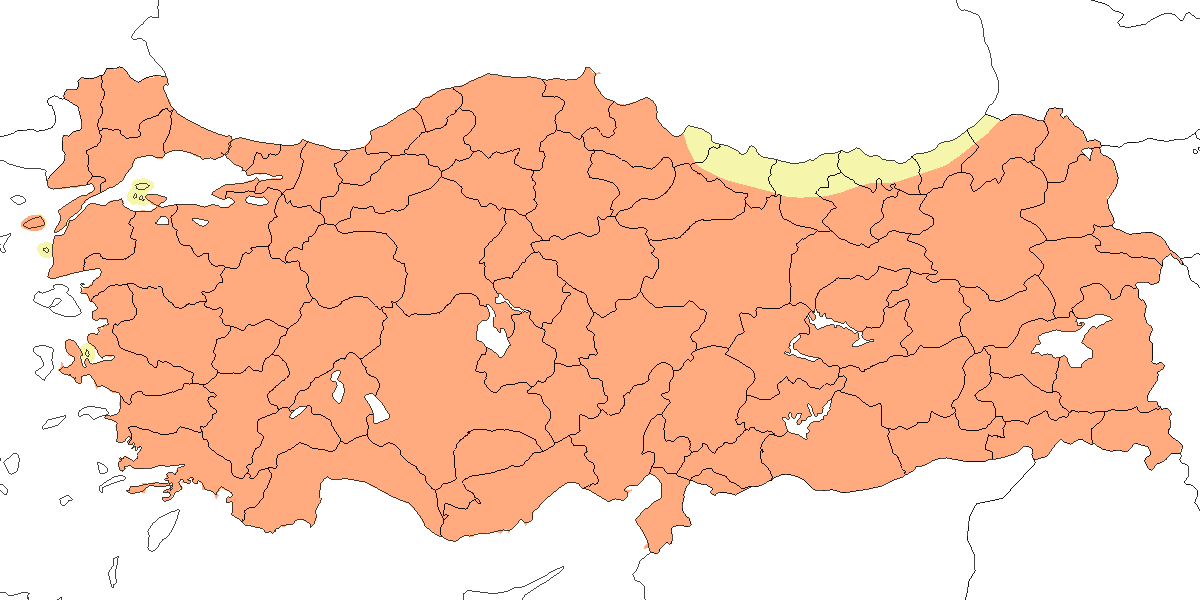
\includegraphics[keepaspectratio]{images/harita_Upupa epops.png}}

\textbf{Üreme}

\textbf{Yuvalama alanı:} İç Anadolu'da küçük yerleşimlerde çatılarda ve
taş yığınlarında, tarihi mesire yerlerinde, kovukların olduğu açık
ağaçlık alanlarda ve bozkırda bulunur.\\
\textbf{Yuvası:} Ağaçkakanların eski yuva delikleri dâhil olmak üzere
ağaçlardaki ve kayalıklardaki deliklerde, kiremitlerin altında,
binalarda ve kuşların yumurtlayabileceği şekilde taş yığınlarındaki ve
duvarlardaki deliklerde yuva yapar. Yuva malzemesi kullanmaz. Yavrularla
birlikte dışkılar yuvada birikir ve kötü kokar.\\
\textbf{Yumurta sayısı:} Türkiye'de gözlenen yumurta sayısı 7 yumurta
ile iki yuvada kaydedilmiştir. Yavru sayısı bir yuvada 2, bir yuvada 4
ve iki yuvada 7 olarak belirlenmiştir.\\
\textbf{Üreme dönemi:} Çoğunlukla mayıs sonu ile haziran ortası arasında
yuva deliklerine yiyecek taşıyan erişkinler gözlenmiştir. Üreme
tarihleri arasında büyük çeşitlilik bulunması türün iki kez kuluçkaya
yatabileceğini göstermektedir. Bu özellik diğer bölgelerde de ara sıra
görülür. \textbf{MAR:} 13 Haziran 1966'da Manyas Gölü'nde bir çift ve 2
tüylenmiş yavru gözlenmiştir. \textbf{EGE:} 20 Mayıs 1999'da Akköy'de
bir erişkinin ağaçtaki delikten dışarı çıktığı görülmüştür. 12 Mayıs
1970'te Altınova'daki bir yuvada yavru kaydedilmiştir. \textbf{AKD:} 7
Mayıs 2004'te Uzuncaburç yakınlarındaki bir kayalıkta yavrularını
besleyen erişkinler gözlenmiştir. \textbf{KAR:} Kızılırmak Deltası'nda
Temmuz 1971'de yavrulu 2 yuva, 8--9 Haziran 1969'da tüylenmiş
yavrularıyla 2 çift (Dijksen \& Kasparek, 1985), 19 Temmuz 1975'te 3
çiftin yavrularını beslediği gözlenmiştir. 1992'de Yörükler Ormanı'nda
33 ve çevresinde 12 territoryum kaydedilmiş, birinde 10 Haziran'da
yavrulu yuva bulunmuştur (Hustings \& Dijk, 1994). \textbf{İÇA:} 11
Mayıs 1993'te Eşmekaya'daki bir kaya yığınının içindeki yuvada 3
yumurta, 16 Mayıs'ta 5 yumurta, 27 Mayıs'ta 6 yumurta ve bir yeni
yumurtadan çıkmış yavru, 30 Mayıs'ta ise tüm yavruların yumurtadan
çıkmış olduğu kaydedilmiştir. 14 Mayıs 2004'te Bolluk Gölü yakınlarında
yumurtlamanın nisan sonunda olduğunu gösteren yeni çıkmış bir yavru
görülmüştür. 8 Mayıs 2005'te Kulu Gölü yakınlarındaki yuvada 6 yumurta
ve bir yeni çıkmış yavru, 14 Mayıs'ta ise 7 yavru kaydedilmiştir. 17
Mayıs 1979'da Sultansazlığı'nda büyük bir yavru ve 10 Haziran 1982'de
uçan bir yavru gözlenmiştir (Kasparek, 1985). 20--27 Haziran 1981'de
Kızılcahamam'daki bir yuvada 2 yavru kaydedilmiştir (Barış, Akçakaya \&
Bilgin, 1984). Ankara'da 22 Temmuz 1969'da 3 yavrusunu besleyen bir çift
ve 2 Temmuz 1968'de bir çift ve genç gözlenmiştir. \textbf{DOA:} 11
Haziran 2001'de Van yakınlarında yavrulu bir yuva, 28 Mayıs 1969'da
Erçek Gölü'nde yavrusunu besleyen bir çift ve 5 Temmuz 2004'te Erzincan
yakınlarında Fırat kıyısında bir aile grubu gözlenmiştir. \textbf{GDA:}
4 Haziran 2001'de Birecik'te eski bir Alaca Ağaçkakan yuvasında 4 büyük
yavru kaydedilmiştir. 26 Nisan 1981'de Birecik'te yumurtlamanın nisan
başında olduğunu gösteren yavrulu yuvaya yiyecek taşıyan bir çift
gözlenmiştir.

\textbf{Alttürler ve Sınıflandırma}

Türkiye'de nominat alttürü bulunur.

\section{Yeşil Arıkuşu}\label{yeux15fil-arux131kuux15fu}

\emph{Merops persicus}, Blue-cheeked Bee-eater

\textbf{\emph{Lokal olara az sayıda yaz konuğu, nispeten yaygın olarak
görülen az sayıda geçit türüdür.}}

Güneydoğu Anadolu'daki kuru ve açık tarım alanlarında üreyen bir yaz
konuğudur. Birecik, Karkamış, Ceylanpınar, Atatürk Barajı, Silopi ve
Karababa Nehri yakınlarında ürediği bilinmektedir. Iğdır yakınlarında da
küçük bir popülasyon bulunmaktadır. Eskiden Birecik ile Karkamış
arasında yaygın olarak ürediği bilinse de, günümüzde bu bölgede
neredeyse yok olmuştur. Buna karşılık Bozova Estağfurullah Köyü'nde hâlâ
düzenli olarak yuvalar. Akdeniz'in komşu bölgelerinde, örneğin Amik Gölü
çevresinde ve Iğdır yakınlarındaki Aras Vadisi'nde de gözlenmiştir.

İlkbahar geçişi nisan başından mayıs sonuna kadar sürer. Bu dönemde
Kızılırmak Deltası, İstanbul Riva ve Ankara Mogan Gölü'nde
kaydedilmiştir. Sonbaharda ağustos ortasından ekim sonuna kadar Çukurova
ve Göksu deltalarında, ayrıca Doğu Anadolu'da Erzurum ve Ani (Kars)
çevresinde zaman zaman daha yaygın görülür. Bu bölgede bazen yüksek
sayılara ulaşabilir (Balmer \& Betton, 2005a, 2008; Vielliard, 1968).
Aynı dönemde Mogan Gölü'nde ve daha nadir olarak İzmir (Krüper, 1875) ve
Sardis çevresinde (Kumerloeve, 1961) kaydedilmiştir.

\pandocbounded{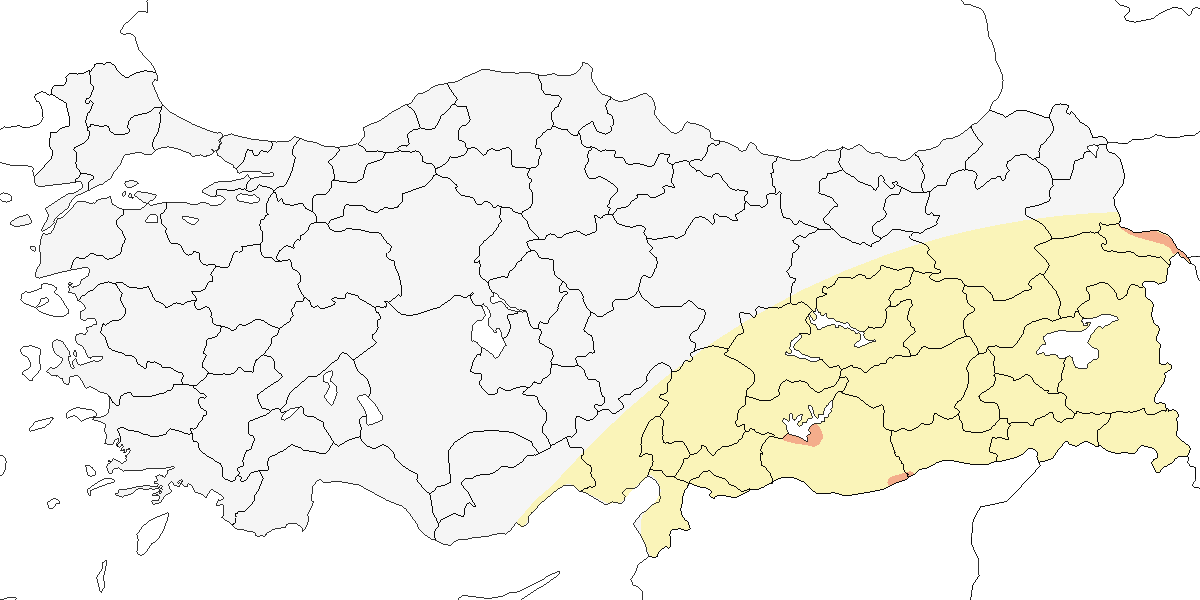
\includegraphics[keepaspectratio]{images/harita_Merops persicus.png}}

\textbf{Üreme}

\textbf{Yuvalama alanı:} Suya yakın açık ve kuru alanlarda, seyrek
ağaçlık alanlarda, plantasyonlarda ve Birecik'te yerleşimlerin
yakınlarında ürer.\\
\textbf{Yuvası:} Seddelerde, kanallarda ve kum ocaklarında yuva yapar.
Bozova'daki yuva höyüklerdedir. Suvat genellikle alçak olur ve toprak
seviyesinden yalnızca biraz yüksektedir. Seddeye yatay olarak kazılmış
1--2 metre uzunluğundaki tünelin ucunda kaplanmamış bir yuva odası
bulunur.\\
\textbf{Yumurta sayısı:} Türkiye'de gözlenen yumurta sayısı 2'dir. Bu
kuluçka 15 Mayıs 1882'de Anadolu'dan alınmış ve muhtemelen
tamamlanmamıştır. Diğer yerlerde genellikle 4--5 yumurta bırakır.\\
\textbf{Üreme dönemi:} Birecik'teki veriler üreme döngüsünün şu şekilde
gerçekleştiğini göstermektedir: Mayısın ikinci yarısında yuva yapımı,
haziran başında yumurtlama (yaklaşık 5 gün), haziranın büyük bölümünde
kuluçka (18--19 gün), haziran sonunda yumurtadan çıkış, temmuzda yuvada
yavruların büyümesi (yaklaşık 27--29 gün) ve temmuz sonunda yavruların
tüylenmesi. \textbf{AKD:} 2 Mayıs 1970'te Amik Gölü yakınlarında, bir
tarım alanındaki kum bankında tünel kazan bir erişkin kaydedilmiştir. 7
Temmuz 1990'da (Eames, 1991) ve 26 Haziran 2005'te Iğdır'ın doğusunda
ürediğinden şüphelenilmiştir. \textbf{GDA:} Birecik'te 18 Mayıs 1993'te
yuva kazma aşamasındaki üç çift ve 28--31 Mayıs 1984'te bir çift
gözlenmiştir. 26 Mayıs 1991'de yuva kazan 12 birey kaydedilmiş, 27 Mayıs
1991'de kur davranışı ve çiftleşme gözlenmiştir. 3 Temmuz 1970 ve 6
Temmuz 1973'te yuvadaki yavrularına yiyecek taşıyan erişkinler
gözlenmiştir. 26--27 Temmuz 1994'te tüylenmiş bir yavru yuvayı terk
etmiştir. 7--8 Ağustos 1988'de erişkinler hâlâ gözlenmiş, ancak 9
Ağustos 1998 ve 10 Ağustos 1989'da kolonilerin terk edildiği
kaydedilmiştir.

\textbf{Alttürler ve Sınıflandırma}

Türkiye'de nominat alttürü bulunur.

\section{Arıkuşu}\label{arux131kuux15fu}

\emph{Merops apiaster}, European Bee-eater

\textbf{\emph{Yaygın ve çok sayıda bulunan yaz konuğu ve geçit
türüdür.}}

Deniz seviyesinden en az 2400 metreye kadar çıkar, ancak genellikle daha
düşük rakımlarda ürer. Güney ve batı bölgelerde nisan sonundan itibaren,
doğu ve kuzeyde ise daha geç dönemde üremeye başlar. Güneyin bazı
bölgelerinde nadir ve daha lokal olarak görülür.

Geçiş dönemlerinde ülke genelinde yaygın ve bol olarak görülür. İlkbahar
geçişi nisan ortasından haziran başına kadar sürer, İç Anadolu'da
genellikle mayıs ortasında tamamlanır. Karadeniz'e nadiren nisan
sonundan önce ulaşır, en yüksek sayılar ise mayıs ortasında kaydedilir
{[}Albrecht (1986); @hustings1994{]}. Sonbaharda ağustos ortasından
eylül sonuna kadar geçiş yapar. 1966'da İstanbul Boğazı'nda 13
Ağustos'tan 24 Eylül'e kadar kaydedilmiş, düzenli olarak ekim sonuna
kadar Trakya'da ve güneyde nadiren kasım ortasına kadar gözlenmiştir.
Tüm ana gözlem noktalarında bol olarak görülen bir geçit türüdür.
Örneğin, 1976'da ağustos sonu ve eylülde Belen Geçidi'nde toplam 1928
birey sayılmıştır (Sutherland \& Brooks, 1981). V. van den Berk ve
arkadaşları (yayınlanmamış) 24 Eylül--3 Ekim 1980 tarihleri arasında
Borçka'dan geçen binlerce kuş kaydetmiştir. Mayıs 2004'teki ilkbahar
gözlemleri, bu türün Doğu Anadolu'nun birçok noktasında sıradan
olabileceğini göstermektedir.

Güneyin bazı kısımlarında nadir ve daha lokaldir. Deniz seviyesinden en
az 2400 m'ye kadar, genelde düşük yüksekliklerde, güneyde ve batıda
nisan sonundan itibaren, doğuda ve kuzeyde ise daha geç üremeye başlar.

\pandocbounded{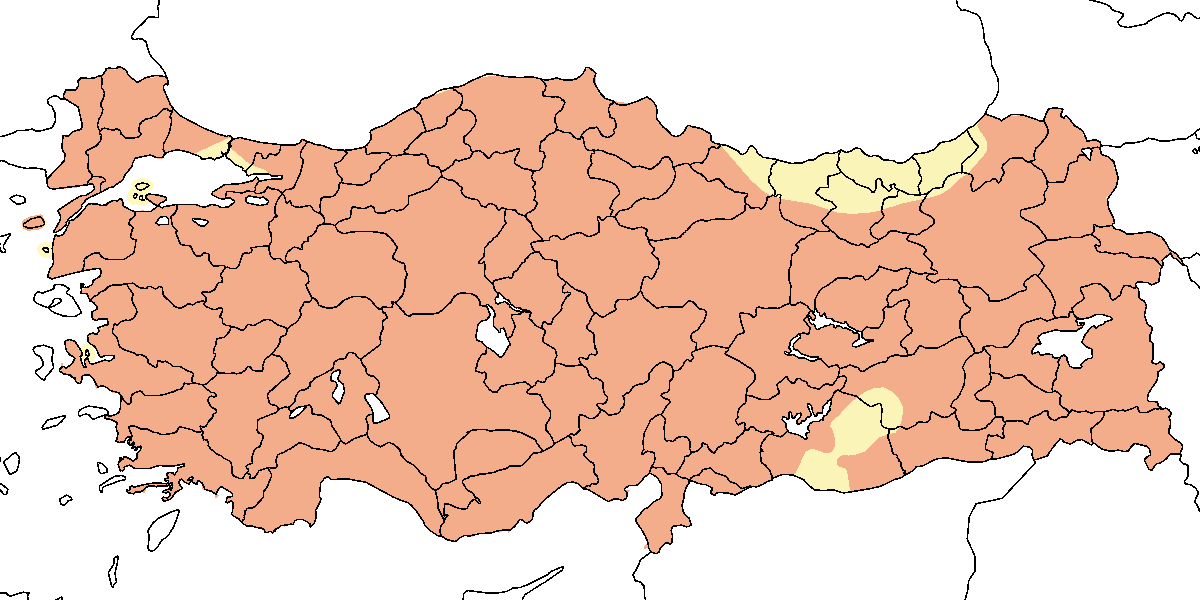
\includegraphics[keepaspectratio]{images/harita_Merops apiaster.png}}

\textbf{Üreme}

\textbf{Yuvalama alanı:} Açık alanlarda, özellikle nehir kıyılarında,
vadilerde ve ovalarda ürer. Ayrıca ekili arazilerde, çalılıklarda, açık
ağaçlık alanlarda ve köy çevresinde de yuvalar.\\
\textbf{Yuvası:} Nehir kıyılarında, yol kenarlarında, kum ocaklarında,
toprak yığınlarında ve kumullarda yuva yapar. 15 Mayıs 2007'de Akköy'de
ve 2020'lı yıllarda İstanbul Riva'da düz zemine kazılmış bir yuva tüneli
gözlenmiştir. Eski yuva tünelleri sonraki yıllarda kaya serçesi, ev
serçesi, ağaç serçesi ve genişletilmiş deliklerde gökkuzgun tarafından
kullanılabilir. Tring Doğa Tarihi Müzesi'ndeki beş yumurtalı bir kuluçka
1 Haziran 1887'de Anadolu'da 2,5 m uzunluğundaki bir tünelden
alınmıştır.\\
\textbf{Yumurta sayısı:} Türkiye'de güncel kayıt bulunmamaktadır. Diğer
yerlerde genellikle 4-7 yumurta bırakır.\\
\textbf{Üreme dönemi:} Üreme dönemi genel olarak mayıs ortasında başlar.
Yumurtlamanın 21 Mayıs'ta gerçekleştiği varsayıldığında, yavrular
haziran ortasında yumurtadan çıkar ve temmuz ortasında tüylenmiş olur.
Türkiye'de tüylenmiş yavruya dair kayıt bulunmamaktadır. Üreme döngüsü
yaklaşık 50 gün sürer. \textbf{MAR:} 23 Haziran 1973'te Enez ve
Keşan'da, 26 Haziran 1973'te Gülpınar'da yuva deliklerine yiyecek
taşıyan erişkinler gözlenmiştir. \textbf{EGE:} 23 Nisan--10 Mayıs 2003
tarihleri arasında Akköy yakınlarındaki iki küçük koloniye günlük
ziyaretler yapılmıştır. 30 Nisan ve 1 Mayıs'ta ilk kuşlar gözlenmiş, 4
Mayıs'ta yaklaşık 10 çiftlik bir kolonide bir çiftin 2,5 m uzunluğunda
yeni bir tünel kazmaya başladığı kaydedilmiştir. 9 Mayıs'ta birçok
erişkinin tünel kazdığı gözlenmiştir. 21 Mayıs 1951'de İzmir civarında
tamamlanmamış bir kuluçkada bir yumurta bulunmuştur (McNeile, 1950,
1951, 1954, 1967, 1968, 1970, 1972, 1973). \textbf{AKD:} 1987'de
Çukurova'da 10 Nisan'dan itibaren erişkinler gözlenmiş, 6 Mayıs'tan
itibaren küçük kolonilere yerleştikleri görülmüştür. \textbf{DOA:} 26
Mayıs 1969'da Van Gölü'nde yuva yapımı gözlenmiştir. \textbf{GDA:} 4
Mayıs 2003, 11 Mayıs 2004 ve 28 Mayıs 1991'de Birecik'te kayıt
alınmıştır.

\textbf{Alttürler ve Sınıflandırma}

Monotipik bir türdür.

\section{Güneyli Yakut Renkli
Arıkuşu}\label{guxfcneyli-yakut-renkli-arux131kuux15fu}

\emph{Merops nubicoides}, Southern Carmine-coloured Bee-eater

\textbf{Rastlantısal konuktur.}

19 Mayıs 2023'te Kızılırmak Deltası'nda bir birey kaydedilmiştir. Türün
doğal yayılış alanı Güney Afrika'dır. Bu nedenle bir hayvanat
bahçesinden kaçmış olma ihtimali değerlendirilmiş, Avrupa'da yalnızca
birkaç hayvanat bahçesinde bulunduğu tespit edilmiştir. Bu kurumlardan
kaçıp Türkiye'ye ulaşmasının düşük olasılık taşıdığı düşünülmüş,
gözlendiği alan da dikkate alınarak bireyin yabani olduğuna ve türün
Türkiye tür listesine dahil edilmesine karar verilmiştir.

\textbf{Üreme}

Türkiye'de yuvalamaz. Yayılış alanı Güney Afrika'dır.

\textbf{Alttürler ve Sınıflandırma}

Monotipik bir türdür.

\section{Yalıçapkını}\label{yalux131uxe7apkux131nux131}

\emph{Alcedo atthis}, Common Kingfisher

\textbf{\emph{Lokal olarak az sayıda üreyen, yaygın ve çok sayıda
bulunan geçit türü ve kış konuğudur.}}

Ülkenin büyük bölümündeki sulakalanlarda ve nehir kenarlarında,
genellikle lokal ve az sayıda bulunan yerli bir türdür. Doğu Anadolu'da
çok daha lokaldir ve İç Anadolu'nun büyük kısmında üremez. Üremesi
nadiren kanıtlanmıştır.

Geçit dönemlerinde ülke genelinde daha yaygın ve genellikle daha boldur.
İlkbahar göçü marttan mayıs sonuna kadar sürer; Karadeniz'de geçişin
nisan ortasında yoğunlaştığı düşünülmektedir. Sonbahar göçü ağustos
sonundan itibaren başlar, kıyı alanlarında eylül sonuna kadar sürer. 20
Ekim ile 18 Kasım arasında en yoğun geçiş gözlenir, geçit bazı bireyler
için aralık sonuna kadar uzayabilir (Albrecht, 1986). Kış döneminde
dağılımı büyük oranda Batı ve Orta Anadolu ile sınırlıdır. Göksu
Deltası, Çukurova Deltası ve Kızılırmak Deltası gibi bazı kıyı
alanlarında önemli sayılarda kışladığı kaydedilmiştir. Bu lokalitelerde
toplamda 1000--2000 birey gözlenmiştir. Rusya'da halkalanmış bir birey
Kızılırmak Deltası'nda tekrar yakalanmış, 2003'te ise muhtemelen daha
kuzeyden gelen bir birey Kızılırmak Deltası'nda halkalandıktan üç gün
sonra Çukurova Deltası'ndaki Akyatan'da tekrar yakalanmıştır (Gürsoy
\emph{vd.}, 2004).

\pandocbounded{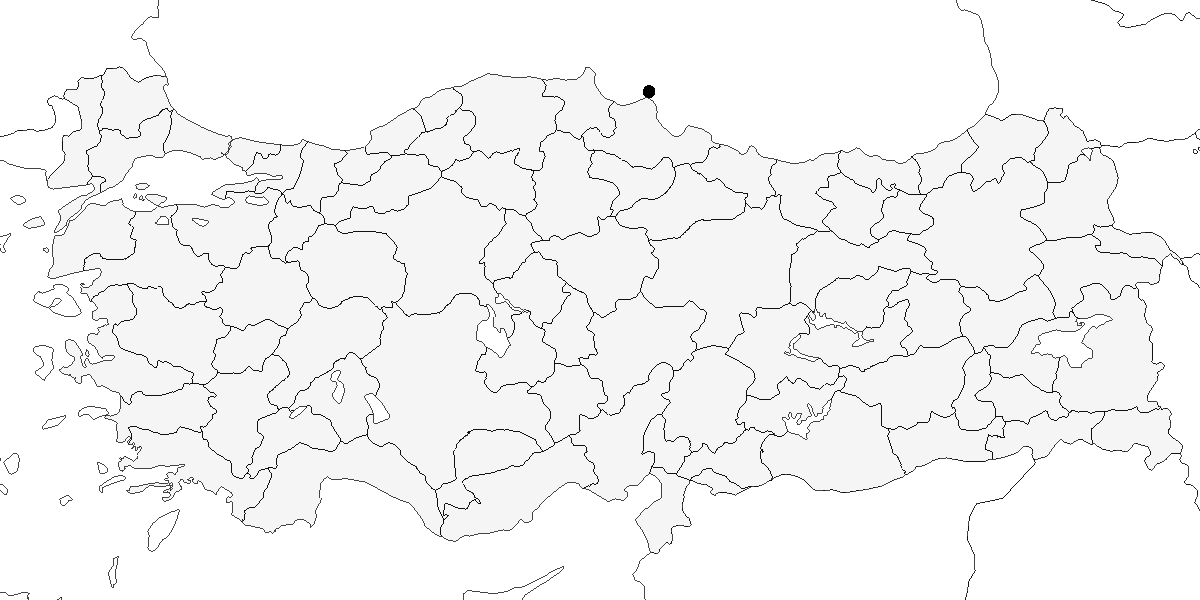
\includegraphics[keepaspectratio]{images/harita_Merops nubicoides.png}}

\textbf{Üreme}

\textbf{Yuvalama alanı:} Nehirler ve dereler boyunca ürer.\\
\textbf{Yuvası:} Erişkinler, dikey kıyılara tünel kazar. Tünel, hafifçe
yukarı doğru eğim yaparak kaplanmamış yuva odasına ulaşır. Yuva tabanı,
yığılmış balık kılçıklarıyla zamanla düzleşir.\\
\textbf{Yumurta sayısı:} Türkiye'de yumurta sayısına dair veri
bulunmamaktadır. Diğer yerlerde genellikle 6-7 yumurta bırakır, bu sayı
4 ile 8 arasında değişebilir.\\
\textbf{Üreme dönemi:} Şubat sonunda yumurtlar. Yavrular mart
sonu--nisan başında yumurtadan çıkar ve mayıs--haziran aylarında yuvadan
ayrılır. \textbf{MAR:} 30 Mayıs 1970'te Lüleburgaz'da yavrusunu besleyen
bir çift gözlenmiştir. \textbf{EGE:} 5 Haziran 1971'de Yatağan'da kayıt
vardır. \textbf{KAR:} Mayıs ayında Fırtına Vadisi'nde kullanılan yuvalar
kaydedilmiştir (Faldborg, 1994). 16 Haziran 1975'te Çaykara'nın
kuzeyindeki bir nehirde, bir erişkinin yiyecek taşıdığı ve bir diğerinin
bunu talep ettiği gözlenmiştir. 13--14 Nisan 1993'te Karpuz Nehri'nin
ağzında genç bireyler dâhil olmak üzere beş birey gözlenmiştir.
\textbf{İÇA:} 16 Mayıs 1970'te Kızılcahamam yakınlarında kayıt
alınmıştır. \textbf{GDA:} 4 Haziran 1969'da Yüksekova'da gözlenmiştir.

\textbf{Alttürler ve Sınıflandırma}

Üreme sezonunda muhtemelen nominat alttür bulunur. Buna karşılık,
Kuzeybatı Afrika ve İspanya'dan Rusya'ya kadar görülen ve Kıbrıs ile
Irak'ta kışlayan \emph{ispida} alttürü, kış döneminde Türkiye'de yüksek
sayılarda bulunuyor olabilir.

\section{İzmir Yalıçapkını}\label{izmir-yalux131uxe7apkux131nux131}

\emph{Halcyon smyrnensis}, White-throated Kingfisher

\textbf{\emph{Lokal ve yer yer çok sayıda bulunan bulunan yerlidir.}}

En önemli üreme alanı, en az 40-45 çiftle Berdan (Tarsus) Nehri'dir.
Göksu Nehri üzerinde Silifke ile Kurtuluş arasında, nehir kıyısındaki
alanlarda beş yuva ve nehrin doğusundaki tarım alanlarında üç
territoryum belirlenmiştir. Ege Bölgesi'nde Bafa Gölü çevresi ve Söke
yakınlarında da yuvalama kaydedilmiştir. Antalya yakınlarındaki Aksu
Nehri'nde kur davranışı gözlenmiştir. 1980-1981'de Bafa Gölü'nde,
1980'den itibaren de Söke çevresinde ürediği teyit edilmiştir.

Onsekizinci yüzyılın başlarında William Sherard'ın İzmir'den aldığı
örnekler Linnaeus tarafından tanımlanmıştır. Ayrıca bu bölgede
kaydedilmiş, İzmir çevresindeki başlıca nehirler boyunca ürediği
belirtilmiştir (Krüper, 1875). Krüper, Mayıs 1894'te bir kuluçka
yumurtası toplamıştır. Ancak bu tarihten sonra bölgede doğrulanmış tek
kayıt, 2002/03'te Çamaltı yakınlarındandır. Kur davranışı sırasında
toplanmış Ege Üniversitesi'ndeki örnek muhtemelen komşu alanlardan
toplanmış olabilir (Berk \& Kasparek, 1988). Büyük Menderes Vadisi'nin
aşağı kesimlerinde Danford ve Selous bu türün varlığını bildirmiştir.
Son yıllarda Güllük Deltası'nda da kaydedilmiştir. Burası görünüşe göre
bilinen en kuzey üreme alanıdır. Haziran 1990'da Troya'da (Çanakkale,
Marmara) uygun habitatta gözlenen bir çift (Deppe, 1990) ve Şubat
2003'te Gediz Deltası'nda gözlenen bir birey bu tespiti
desteklemektedir.

Üreme dönemine ait olmak üzere, Fırat ve Dicle nehirleri ile Cizre ve
Siirt'e kadar Güneydoğu Anadolu'da beş kayıt bulunmaktadır. En önemli
üreme alanları Akdeniz Bölgesi'ndedir. Köyceğiz Gölü çevresinde birkaç
çift, Göksu Nehri'nin aşağı kesimlerinde son yıllarda 8--10 çift (Berk
\& Guder, 1992), en büyük popülasyonlar ise Tarsus'ta (1987'de 40--45
çift) ve Ceyhan Deltası'nda yer alır. Tahminlere göre Türkiye'de toplam
100--150 çift üremektedir (Berk \& Kasparek, 1988). Yoğun tarım
faaliyetlerinin Çukurova'daki popülasyona olumlu etkisi olmasına rağmen,
diğer bölgelerde uzun vadeli bir azalma eğilimi gözlenmektedir. Küçük
Menderes Deltası (İzmir) ve artık kurutulmuş olan Amik Gölü (Antakya)
gibi eski üreme alanları terkedilmiş, Göksu Deltası'ndaki popülasyon da
geçmişe göre küçülmüştür.

Bilinen üreme alanları dışındaki bazı kayıtlar, özellikle ağustos sonu
ile şubat sonu arasında gözlendiğinden, türün üreme dönemi dışında Ege
ve Akdeniz bölgelerinde sınırlı ve muhtemelen düzensiz bir yayılış
gösterdiğini düşündürmektedir. İstanbul'dan bildirilen iki kayıt
(Rigler, 1852) ve (Wahby, 1930) şüpheli kabul edilmektedir. Kesin
olarak, 17 Aralık 2001'de Nevşehir'de, Avanos'ta Kızılırmak kıyısında
bir birey kaydedilmiştir.

\pandocbounded{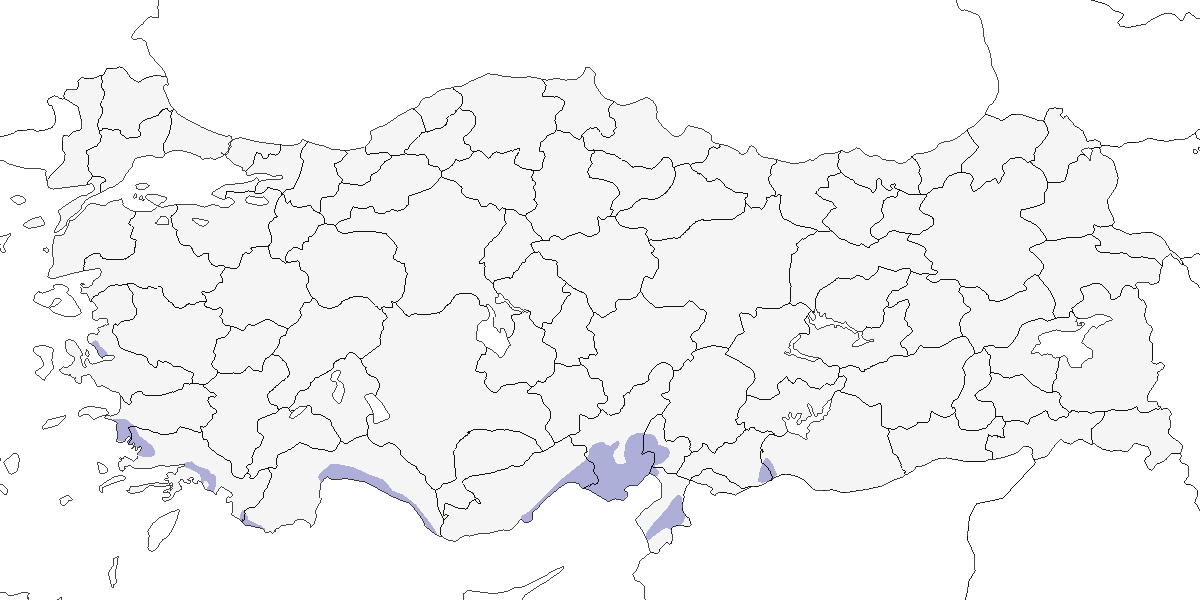
\includegraphics[keepaspectratio]{images/harita_Halcyon smyrnensis.png}}

\textbf{Üreme}

\textbf{Yuvalama alanı:} Akdeniz'de (özellikle Çukurova ve Göksu
deltalarında) ve az sayıda Ege'deki kıyısal ovalardaki nehir boylarında
ve çevresindeki ağaçlık bölgelerde ürer.\\
\textbf{Yuvası:} Yuvayı dik nehir kıyılarındaki tünel biçiminde
oydukları deliklerin ucunda oluşturur. Tünelin ucunda yer alan yuva
odası kaplanmamıştır. Yuva tünellerinin uzunluğu 60-80 cm arasında
değişir.\\
\textbf{Yumurta sayısı:} Bir yuvada 5 yumurta, iki yuvada 6 yumurta
tespit edilmiştir. Bir yuvada ise 3 yumurtalı tamamlanmamış bir kuluçka
kaydedilmiştir. Yavru sayısı bilinmemektedir.\\
\textbf{Üreme dönemi:} Nisan başında yuva deliklerinin önünde kur
davranışı gözlenmiştir. 27 Nisan 1965'te tamamlanmamış ve tamamlanmış
kuluçkalar kaydedilmiştir. 6 Mayıs 1964'te taze yumurtalı iki
tamamlanmış kuluçka bulunmuştur. 21 Mayıs 1974'te yuvadaki yavrulara
küçük kertenkeleler ve dikenli keler taşıyan erişkinler gözlenmiştir. 12
Haziran 2002'de bir yuva deliğinde bir erişkin, 10 Temmuz 1991'de
kıyıdaki olası bir yuvaya giren başka bir erişkin kaydedilmiştir.
Yumurtlamanın nisan ayı sonunda başladığı, yavruların haziran ortasında
yuvada olduğu anlaşılmaktadır. \textbf{EGE:} 4 Mayıs 1894'te İzmir
yakınlarında Krüper tarafından bir kuluçka toplanmıştır; 1980-81'de Bafa
Gölü'nde üremiş ve 1980'den bu yana Söke yakınlarında ürediği birkaç
defa teyit edilmiştir. Yuvası, bir tünelin ucunda kaplamasız bir
bölmedir (Harrison \& Castell, 2002). \textbf{AKD:} Üreme biyolojisi
kapsamlı şekilde araştırılmıştır (Berk \& Kasparek, 1988). En önemli
üreme alanı en az 40-45 çift ile Berdan (Tarsus) Nehri'dir (Çukurova).
Nehir kıyısı 4 m kadar yüksektir ve 12-13 Mayıs 1987'de dış menderes
kıyısında birbirinden 200-800 m mesafede 19 tane kullanılan yuva
bulunmuştur (Berk \& Kasparek, 1988). Ormanlık alanda yok kenarındaki
bankette de iki yuva daha kaydedilmiştir (Have \emph{vd.}, 1988). Nisan
başında yuva deliklerinin önünde kur davranışları gözlenmiştir. 27 Nisan
1965'te üç yumurtalı tamamlanmamış bir kuluçka ve beş yumurtalı
tamamlanmış bir kuluçka bulunmuştur; 6 Mayıs 1964'te altı yumurtalı
(biri taze) tamamlanmış iki kuluçka bulunmuş ve yuva tünelinin uzunluğu
60-80 cm olarak ölçülmüştür (Warncke, 1964-\/-65). 21 Mayıs 1974'te
Mersin yakınlarında yuvadaki yavrularına küçük kertenkeleler ve dikenli
keler taşıyan erişkinler gözlenmiştir. 1989 ve 1991'de Göksu Nehri
üzerinde Silifke ile Kurtuluş arasında beş yuva kaydedilmiş ve nehrin
doğusundaki tarım alanlarında üç territoryum gözlenmiştir; nisan-mayıs
aylarında nehir kıyısında yuvalar bulunmuştur; 12 Haziran 2002'de bir
yuva deliğinde bir erişkin görülmüş ve 10 Temmuz 1991'de bir erişkinin
kıyıdaki olası bir yuvaya girdiği gözlenmiştir. 24 Nisan 1967'de Antalya
yakınlarında Aksu Nehri'nde balık taşıma da dâhil kur davranışları
gözlenmiştir.

\textbf{Alttürler ve Sınıflandırma}

Türkiye'de nominat alttürü bulunur. İzmir'de tanımlanmıştır.

\section{Alaca Yalıçapkını}\label{alaca-yalux131uxe7apkux131nux131}

\emph{Ceryle rudis}, Pied Kingfisher

\textbf{\emph{Lokal ve yer yer çok sayıda bulunan yerlidir.}}

Fırat ve Dicle boyunca yaygın olarak görülen, Ege'nin güneyi ve
Akdeniz'deki sulakalanlar ile kıyısal ovalardaki nehir boylarında,
nispeten lokal ancak nadir olmayan yerli bir türdür. Güneydoğu
Anadolu'daki Fırat ve Dicle gibi büyük nehirler boyunca ve Doğu
Anadolu'nun hemen bitişiğindeki alanlarda yaygındır. Yayılışının kuzey
sınırının Gölbaşı (Adıyaman), Malatya, Diyarbakır ve Bitlis arasında
uzandığı düşünülmektedir. Bazı eski habitatları baraj inşaatları
nedeniyle sular altında kalmış olsa da, yayılışın doğusunda azaldığını
gösteren yeterli veri bulunmamaktadır.

Eskiden Ege ve Akdeniz bölgelerinde daha yaygın ve boldu. İzmir ve
çevresinde birçok gözlemci tarafından kaydedilmiştir ancak artık düzenli
olarak görülmemektedir. Gediz Deltası, Büyük Menderes Deltası ve Güllük
Deltası'nda hâlâ üreyebileceği düşünülmektedir. Akdeniz'de, geçmişte
Amik Gölü ve Göksu Deltası'nda üremiştir. Köyceğiz sulakalan
kompleksinde hâlâ üremekte, ayrıca Çukurova'da da çoğunlukla kış
döneminde gözlenmektedir. Eylül 2004'te Akseki'de bir dişinin
kaydedilmesi, bölgedeki varlığını desteklemektedir.

Genellikle aynı bölgelerde kışın daha yaygın görülür. Bu dönemde daha
geniş çapta dağıldığını gösteren sınırlı sayıda kayıt vardır. Ocak
1969'da Karacabey'de (Balıkesir, Marmara), Aralık 1970'te Denizli'nin
batısında {[}OST (1972); @ost1975{]}, ayrıca Burdur Gölü ve Tuz Gölü'nde
kaydedilmiştir {[}Kasparek (1992); @kumerloeve1961{]}.

\pandocbounded{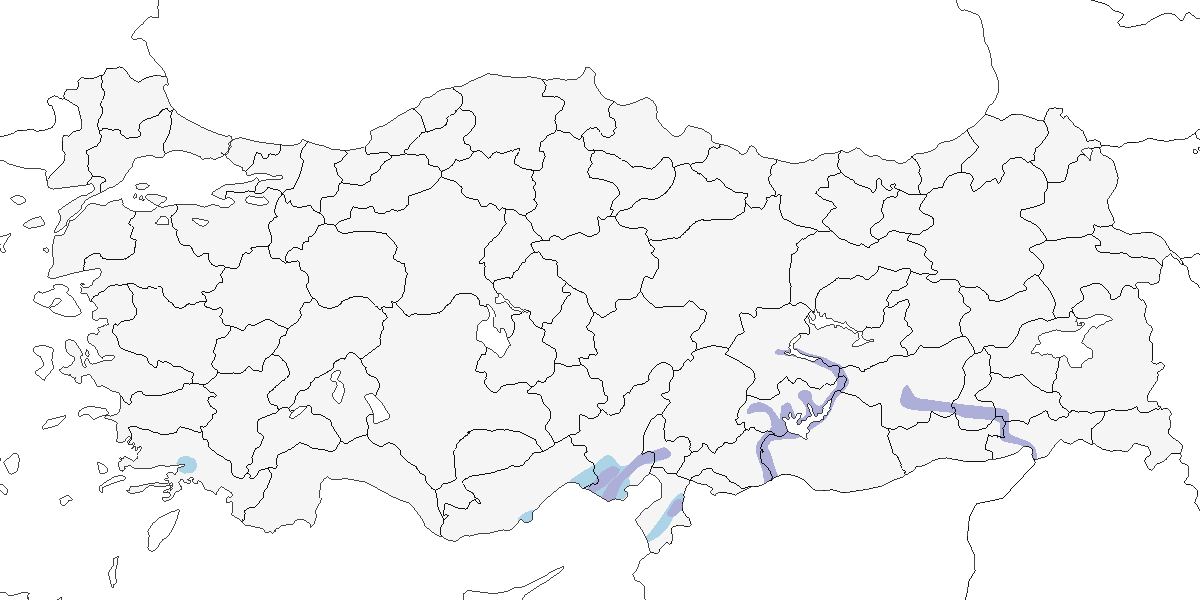
\includegraphics[keepaspectratio]{images/harita_Ceryle rudis.png}}

\textbf{Üreme}

\textbf{Yuvalama alanı:} Fırat ve Dicle gibi büyük nehirler boyunca ve
nehir kıyısındaki gölcüklerde ürer.\\
\textbf{Yumurta sayısı:} Dikey kıyılara kazılan tünellerin sonunda
kaplanmamış bir odacığa yuva yapar. Türkiye'de bir yuvada 6 yumurta
kaydedilmiştir. Diğer yerlerde olağan kuluçka büyüklüğü 3--6, genellikle
4 yumurtadır. Türkiye'de tüylenmiş yavru sayısı 3 ile 5 arasında
değişmektedir.\\
\textbf{Üreme dönemi:} Mayıs sonunda yumurtlar, yavrular haziran sonunda
tüylenir ve temmuz sonunda yuvayı terk eder. \textbf{EGE:} 14 Mayıs
1899'da İzmir yakınlarında bir tünelden altı taze yumurta alınmıştır.
23--27 Haziran 1966'da Büyük Menderes Nehri'nde iki çiftin yuva
deliklerine girip çıktığı, 25--26 Haziran'da ise üç tüylenmiş yavrunun
gözlendiği kaydedilmiştir. \textbf{AKD:} 12 Mayıs 1982'de Göksu'da aktif
bir yuvayı ziyaret eden erişkinler, 1983 Mayıs sonunda Dalyan'da
tüylenmiş üç yavrunun iki erişkini takip ettiği gözlenmiştir.
\textbf{GDA:} 7--18 Ağustos 1971'de Asvan'da iki erişkin ve beş genç
birey kaydedilmiştir. 12 Nisan 1996'da Birecik'te kur davranışı, 20
Mayıs 1993'te tünel kazmaya başlayan bir erişkin ve 5 Haziran 1993'te
kuluçkadaki bir erişkin gözlenmiştir. 24 Temmuz 1998'de altı bireyli bir
aile grubu kaydedilmiştir.

\textbf{Alttürler ve Sınıflandırma}

Türkiye'de \emph{syriacus} alttürü bulunur. İzmir, Antalya ve yeri
bilinmeyen bir lokalite olan ``Harpara''dan elde edilen örneklerde, gaga
uzunluğu dışında tüm ölçümlerin sürekli daha küçük olmasına dayanarak,
Türkiye, Kıbrıs, Doğu Akdeniz, Irak ve İran'daki bireyler için bu yeni
alttür tanımlanmıştır (Roselaar, 1995). Ancak bu öneri, ölçümlerdeki
farklılıkların Bergman kuralıyla açıklanabileceği gerekçesiyle
reddedilmiştir (Kasparek, 1996).

\section{Gökkuzgun}\label{guxf6kkuzgun}

\emph{Coracias garrulus}, European Roller

\textbf{\emph{Oldukça yaygın ve yer yer çok sayıda bulunan yaz
konuğudur.}}

En az 2000 metreye kadar olan açık ve ağaçlık alanlarda, ayrıca seyrek
ağaçlı açık alanlarda, kayalıklarda, ahırlarda ve yıkıntılarda yuvalar.
Orman kenarları, zeytinlikler, bozkırlar ve seyrek ağaçlı tarlalar gibi
farklı habitatlarda da bulunur. Yuva yeri seçimi genellikle uygun
yapısal alanların varlığına bağlıdır. Karadeniz Bölgesi'nde son derece
lokal yayılış gösterir ve bazı alanlarda hiç bulunmayabilir.

Geçiş dönemlerinde ülke genelinde yaygındır. İlkbaharda mart sonundan
itibaren güney kıyılarında gözlenmeye başlar, nisan sonu ile mayıs
başında en yüksek sayılara ulaşır ve ancak bu dönemde kuzey bölgelerde
görülür. Sonbaharda ağustos başından ekim sonuna kadar geçiş yapar.
Eylül ortasında kuzey ve batı bölgelerden çoğunlukla ayrılır, ancak
Akdeniz ve İç Anadolu'da kasım sonuna kadar gözlenebilir.

\pandocbounded{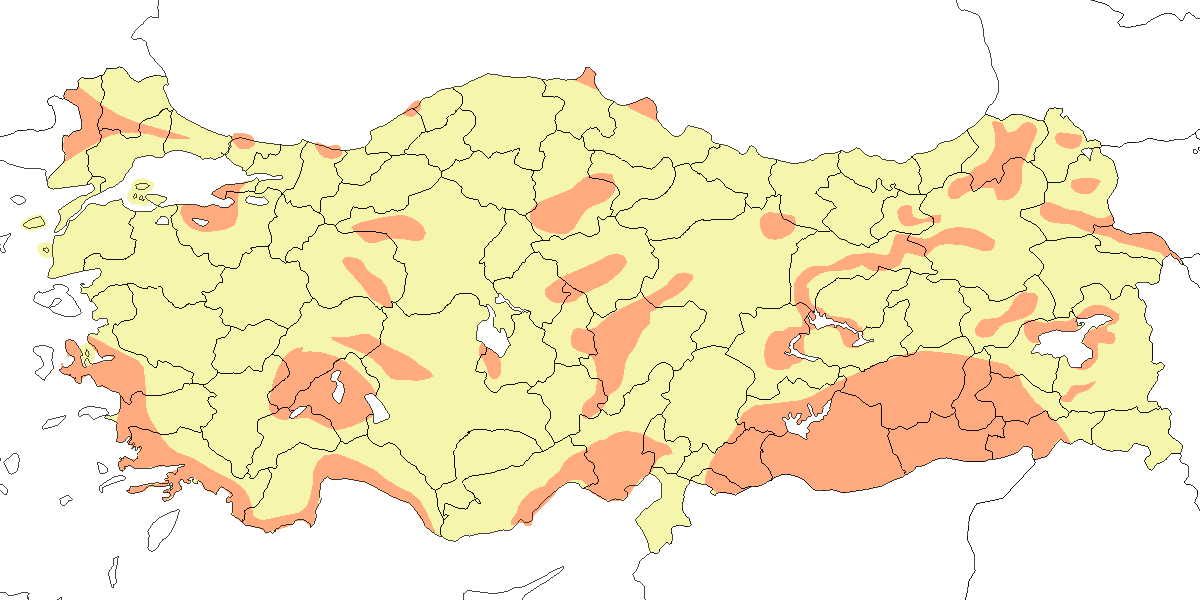
\includegraphics[keepaspectratio]{images/harita_Coracias garrulus.png}}

\textbf{Üreme}

\textbf{Yuvalama Alanı:} Ege ve Akdeniz bölgelerindeki zeytin bahçeleri
ve benzeri açık tarımsal arazilerde, yuva alanı bulabildiği nehir
boyları, deltalar, kum ocakları ve kayalıkların çevresindeki açık
arazide bulunur.\textbf{\hfill\break
Yuvası:} Yuvasını yaşlı ağaçlardaki (özellikle zeytin), kayalıklardaki
oyuklarda, toprak dolgularında, yıkıntılarda, binalarda ve köprülerde
yapar. Yuvalar kaplanmamış bir boşluktur. Efes'te, tarihi bir alanda
kazı çalışmaları için kullanılan bir vincin oyuğunda yuva yaptığı da
kaydedilmiştir. İç Anadolu'da düz, ağaçsız alanlarda yerdeki gelengi
(\emph{Spermophilus xanthoprymnus}) yuvalarını da kullandığı
bilinmektedir.\\
\textbf{Yumurta sayısı:} Türkiye'de gözlenen yumurta sayısı, iki yuvada
üç, bir yuvada dört ve dört yuvada beş olarak kaydedilmiştir.\\
\textbf{Üreme Dönemi:} Yumurtlamanın mayıs başından haziran ortasına
kadar olabildiği göz önüne alındığında Türkiye'de üremenin değişken
olduğu anlaşılmaktadır. Yumurtadan çıkan yavrular genellikle temmuz
başından itibaren gözlenmiştir. \textbf{MAR:} Manyas Gölü'nde, kısmen su
içindeki bir söğütlükte su seviyesinden 1 m yüksekteki bir ağaç
deliğinde 5 Haziran 1966'da bir yumurta ve 9 Haziran 1966'da üç yumurta
bulunmuştur. Aynı tarihlerde benzer bir alanda bir yuvada üç, diğer bir
yuvada bir yumurta kaydedilmiştir. Ağustos 1968 başlarında geç kalmış
bir yuvada hâlâ yavru olduğu görülmüş, 21--27 Haziran 1973'te yiyecek
taşıyan beş çift kaydedilmiştir. \textbf{EGE:} 8 Mayıs 1899'da Aydın
yakınlarındaki kayalıklardan henüz yumurtlamamış birçok erişkin
havalanmıştır. Tring Doğa Tarihi Müzesi'nde yer alan beş, dört ve beş
yumurtalı üç kuluçka sırasıyla 1 Mayıs 1887'de İzmir'den, 19 Mayıs
1901'de Milet harabelerinden ve 29 Mayıs 1901'de Büyük Menderes
Nehri'nden toplanmıştır. 14 Mayıs 1991 ve 19 Mayıs 1999'da erişilemeyen
yuvalarda gözlenen erişkinler büyük olasılıkla kuluçkadaydı. 28 Mayıs
1951'de İzmir yakınlarındaki bir taş köprüdeki bir delikte kuluçkanın
ileri evresinde bulunan beş yumurta, ilk yumurtanın yaklaşık 8 Mayıs'ta
bırakıldığını göstermektedir. \textbf{AKD:} 9 Mayıs 1970'te Adana
yakınlarındaki bir kaya yüzeyindeki yuvada kur davranışı sergileyen bir
çiftin birbirini beslediği görülmüştür. 2 Temmuz 1972'de Side'de, yerden
2,7 m yüksekteki bir çam ağacında en az iki büyük yavru; 24 Mayıs
2007'de Manavgat yakınlarında bir köprüdeki yuvada beş yumurta
gözlenmiştir. \textbf{KAR:} Kızılırmak Deltası'nda, 28 Mayıs 1979'da
ağaçlardaki yuva delikleri için küçük kargalarla kavga eden çiftler;
9-10 Haziran 1975'te kur davranışı sergileyen çiftler; Temmuz 1971'de
yiyecek taşıyan dört çift; 29 Temmuz 1971'de tüylenmiş iki yavru; 5--12
Temmuz 1983'te ise tüylenmiş yavrular kaydedilmiştir. 1992'de kur
davranışları özellikle mayısın ikinci yarısında gözlenmiş, haziranın ilk
on gününde yuvaların yanında alarm ötüşü yapan çiftler rapor edilmiştir.
\textbf{İÇA:} Bir çiftin, 15 çiftlik bir arıkuşu kolonisiyle aynı
suvatta kuluçkaya yattığı bildirilmiştir. Temmuz ve ağustos aylarında
genç bireyler gözlenmiştir. \textbf{DOA:} 8 Haziran 2004'te Van
yakınlarında, kum kırlangıçlarının da kullandığı yol kenarındaki yüksek
bir suvatta geniş bir delikten kuluçkadaki bir erişkin uçmuştur. 24
Haziran 2004'te İspir'de, bir arıkuşu kolonisinin de bulunduğu yol
kenarındaki yüksek bir suvatta geniş bir deliğe giren bir erişkin
gözlenmiştir. Daha sonra aynı yerden iki erişkin gökkuzgunun çıkması,
yuvada büyük yavruların bulunduğunu düşündürmektedir. \textbf{GDA:} 5
Haziran 1998'de Birecik'te bir suvatta tüylenmemiş dört yavru
gözlenmiştir. Aynı yerde, 20 Mayıs 1993 ve 4 Haziran 1998'de erişkinler
yuvada muhtemelen kuluçkadaydı. 20 Mayıs'ta bir yuvada bir yumurta
bulunmuştur. 25 Mayıs 2009'da nehir suvatlarındaki dört yuvadan birinde
beş yumurta görülmüştür.

\textbf{Alttürler ve Sınıflandırma}

Türkiye'de nominat alttürü bulunur.

\section{Hint Gökkuzgunu}\label{hint-guxf6kkuzgunu}

\emph{Coracias benghalensis}, Indian Roller

\textbf{\emph{Rastlantısal konuktur.}}

1875'te Sclater ve Taylor, Haydarpaşa ile İzmit arasında bir birey
topladıklarını bildirmiştir (Sclater \& Taylor, 1876). Bu örnek daha
sonra Pearce'in koleksiyonuna geçmiş, ardından Robert Kolej Müzesi'ne
devredilmiştir. Bu bağlamda, söz konusu örneği tek bir geçerli kayıt
olarak değerlendirmek uygundur. Bu örnek kaydını kabul
görmüştür(Dresser, 1871-\/-1881). Ancak Kumerloeve (1961) bu örnekten
hiç bahsetmemiştir.

Danford (Danford, 1877-78), Giaour Keui (Gavurköy) ile Bereketlu
(Bereketli) arasında bir birey ve Nisan 1876'da Çamardı ile Karanfil Dağ
arasında iki birey daha gördüğünü öne sürmüştür. Ancak bu kayıtlar
döneminde de tartışmalı bulunmuş (Kumerloeve, 1961) ve geçersiz
sayılmalıdır.

\pandocbounded{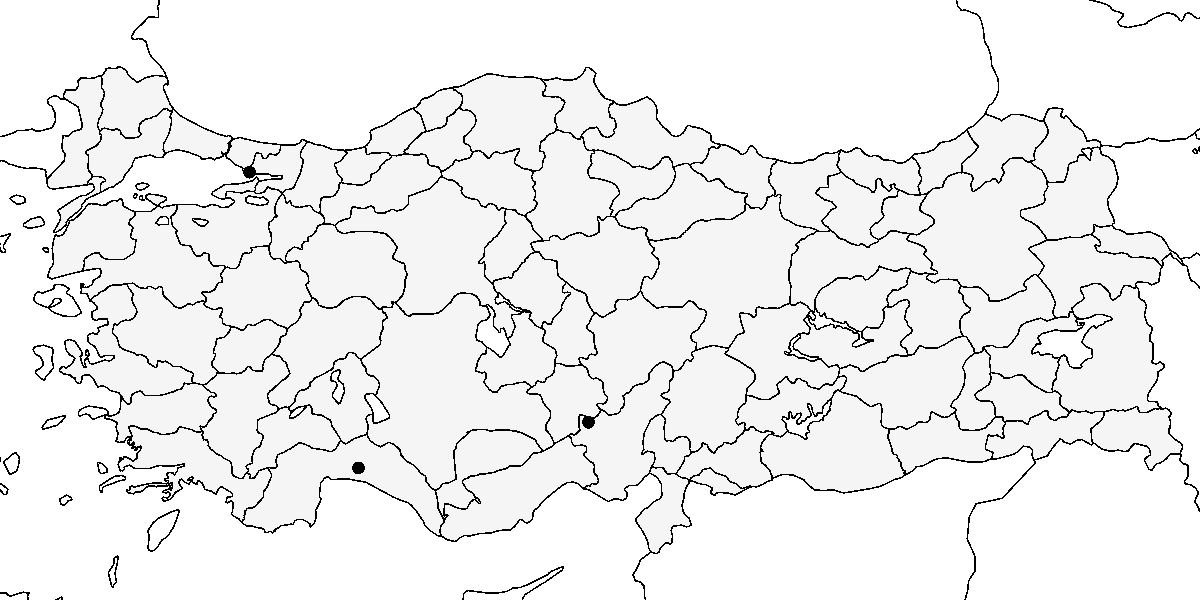
\includegraphics[keepaspectratio]{images/harita_Coracias benghalensis.png}}

\textbf{Üreme}

Türkiye'de yuvalamaz. Yuvalama alanı İran, Pakistan, Hindistan ve
çevresidir.

\textbf{Alttürler ve Sınıflandırma}

Tahnit örneği muhtemelen İran'ın doğusuna kadar yayılış gösteren nominat
alttüre aittir.

\section{Boyunçeviren}\label{boyunuxe7eviren}

\emph{Jynx torquilla}, Eurasian Wryneck

\textbf{\emph{Yerel olarak ve az sayıda görülen yaz konuğu, yaygın ve
nispeten çok sayıda bulunan geçit türü, nadir ve lokal kış konuğudur.}}

Genellikle açık ağaçlık alanlarda, plantasyonlarda ve meyve bahçelerinde
ürer. Batı Karadeniz'de 1700 metreye kadar çıkar. Orta Toroslar gibi
diğer ormanlık bölgelerde az sayıda üreyebilir. Son yıllarda Doğu
Anadolu ve Karadeniz'in doğusunda da üreme sezonunda kaydedilmiştir.
Ege'nin kuzey ve doğusunda da son dönemde az sayıda görülmüştür.
1988-1990 yıllarında Istranca Dağları'nın Bulgaristan tarafında yapılan
çalışmalarda, 5 kilometrelik karelerin \%47'sinde ürediğine dair kanıt
bulunmuş, \%25'inde ise yuvaladığı teyit edilmiştir (Milchev, 1994).
Geçiş yapan kuşlar, üreme yayılışını değerlendirmeyi zorlaştırır.
Karadeniz'de, Kızılcahamam'da ve Uludağ'da da üreme döneminde öten
erişkinler kaydedilmiştir. Kuluçka ve yavru besleme döneminde sessiz
olduğu için gözden kaçabilir ve muhtemelen sanılandan daha fazla sayıda
üremektedir.

Geçiş döneminde özellikle batı ve orta bölgelerde az sayıda kaydedilir.
İç Anadolu'da sonbaharda daha bol olduğu bildirilmiştir (Schekkerman \&
Roomen, 1993). 216 göçmen kaydı üzerinden yapılan analizde, ortalama
geçiş tarihleri 15 Nisan ve 6 Eylül olarak hesaplanmıştır (Kasparek,
1989). İlkbaharda mart başından itibaren görülmeye başlanır, mart sonu
ile mayıs sonuna kadar devam eder. Sonbaharda ağustos başından ekim
başına kadar geçiş yapar ve eylül ortasında belirgin yoğunluk kazanır.
Geçmişte göç sırasında daha kalabalık olduğu düşünülmektedir. Von
Gonzenbach 19. yüzyıl ortasında İzmir'de, Braun ise 20. yüzyıl
başlarında İstanbul'da bu türü bol, hatta çok bol bir göçmen olarak
tanımlamıştır.

Kış döneminde kıyı alanlarında nadiren görülür. Aralık ile şubat
arasında İzmir ile Antakya arasında kaydedilebilir. Kışın, sınırlı da
olsa yer tutma davranışı gösterebilir. Kasım ortasında Side'de, 24
Kasım'da Samandağ'da ve 25 Kasım'da Birecik'te bu şekilde davranan
bireyler gözlenmiştir. Kış dönemine ait en yüksek rakımlı kayıt, 700
metrede Antalya Kemer yakınlarındaki Gedelme'den 26 Aralık 2007 tarihine
aittir (A.-A. Weller).

\pandocbounded{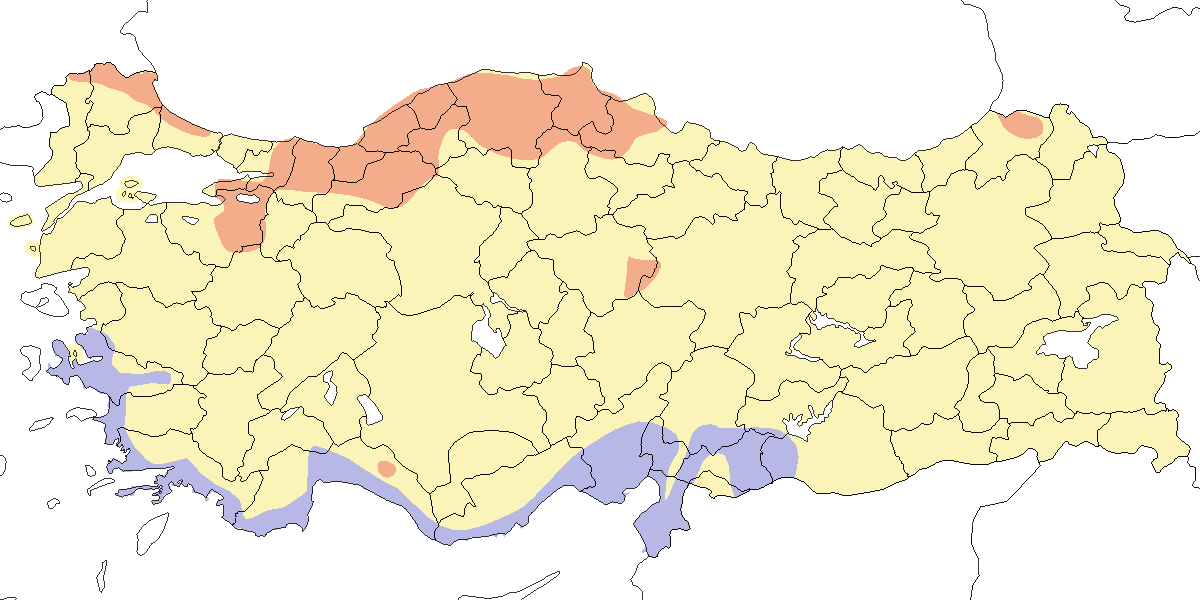
\includegraphics[keepaspectratio]{images/harita_Jynx torquilla.png}}

\textbf{Üreme}

\textbf{Yuvalama alanı:} Ormanlarda, açık ağaçlık alanlarda ve ağaçların
bulunduğu tarım alanlarında yuvalar.\\
\textbf{Yuvası:} Yuvasını ağaçtaki bir deliğe yapar. Yuva, kaplanmamış
bir boşluktur ve hiçbir yuva malzemesi kullanılmaz.\\
\textbf{Yumurta sayısı:} Türkiye'de üç yumurta kaydedilmiştir. Diğer
ülkelerde olağan kuluçka büyüklüğü 7-10 yumurtadır.\\
\textbf{Üreme dönemi:} Yavrular haziran ayında yuvada görülmüş,
yumurtlamanın mayıs sonunda veya haziran başında gerçekleştiği
anlaşılmıştır. \textbf{AKD:} 17 Temmuz 1986'da Akseki'nin 60 km
kuzeyinde, hav tüyleri olan genç bir birey kaydedilmiştir (Martins,
1989). Bu gözlem yumurtlamanın haziran başında olduğunu göstermektedir.
4 Haziran 2000'de Akseki'de bir yuva deliğini inceleyen ve birbirleriyle
etkileşen iki erişkin gözlenmiş, aynı gün yakınlarda öten bir birey daha
kaydedilmiştir. \textbf{KAR:} 11 Haziran 1977'de Ilgaz Dağları'nda
1300-1400 metre yükseklikte, bir yuva deliğinin altında yerde kırılmamış
üç yumurta bulunmuştur. Bu yumurtalardan ikisi biraz kuluçkaya yatılmış,
biri döllenmemiştir. Yumurtalar doğru şekilde tanımlanmıştır. 11-12
Haziran'da aynı bölgede öten beş birey kaydedilmiştir (Schubert, 1979).
16 Nisan 1978'de Ereğli'de bir erişkinin olası bir yuva deliğini
incelediği, 14 Haziran 1978'de aynı yerde iki bireyin ötüşüyle birlikte
üremeden şüphelenildiği bildirilmiştir (Albrecht, 1986). Kızılırmak
Deltası'nda 31 Mayıs 1979'da bir yuvada yavrularını besleyen erişkinler
gözlenmiştir (Dijksen \& Kasparek, 1985).

\textbf{Alttürler ve Sınıflandırma}

Türkiye'de muhtemelen nominat alttür bulunur. Sonbaharda Orta Anadolu
üzerinden geçiş yapan göçmenlerin tamamı bu forma dâhildir (Berk, 1990).
Bununla birlikte, Akdeniz'de Korsika'dan Adriyatik kıyılarına kadar bazı
adalarda üreyen tschusii alttürü göçe yatkın olmasa da (Vaurie, 1959a),
geçiş sırasında Türkiye'de gözlenebilir.

\section{Ortanca Ağaçkakan}\label{ortanca-aux11fauxe7kakan}

\emph{Dendrocoptes medius}, Middle Spotted Woodpecker

\textbf{\emph{Yaygın ve nispeten çok sayıda bulunan yerlidir.}}

Ege ve Akdeniz'in büyük bölümünde oldukça yaygın ve nispeten boldur.
Marmara ve Batı Karadeniz'de daha lokal olarak görülür. Kızılırmak
Deltası'nda 1992 ilkbaharında 20-30 çiftin ürediği tahmin edilmiştir. Bu
sayı, türün üreme yoğunluğuna dair az sayıdaki tahminlerden biridir.
Doğu Anadolu'nun batısındaki ve Karadeniz'in doğusundaki varlığı
{[}Kumerloeve (1961); @kumerloeve1970a{]} tarafından belgelenmiştir.
Ancak ornitolojik araştırmaların yetersizliği ve uygun habitatların
azalması nedeniyle Doğu Anadolu'nun batısında son yıllarda çok az kayıt
vardır. 1993 ilkbaharında Karadeniz'in doğusunda türe rastlanmamıştır
(Faldborg, 1994).

Yaprak döken, nadiren karışık ormanlarda ve zeytinliklerde yaşar. İbreli
ormanlarda nadirdir. Meşe, tercih ettiği habitatın önemli bir unsurudur.
Güneyde ve batıda deniz seviyesinden 800 metreye kadar yayılış gösterir.
Doğu Karadeniz'de ve bazı diğer bölgelerde 1400 metreye kadar çıkabilir.
Kumerloeve ve Niethammer, türü şüpheli şekilde Ilgaz Dağları'nda 1900
metre civarında kaydetmiştir.

\pandocbounded{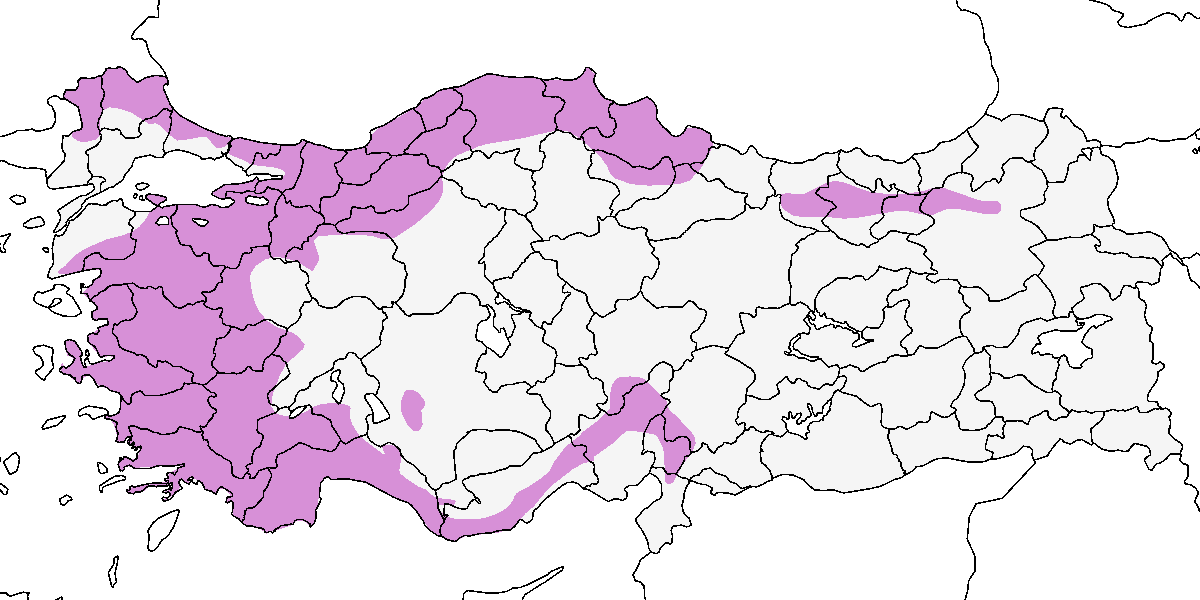
\includegraphics[keepaspectratio]{images/harita_Dendrocoptes medius.png}}

\textbf{Üreme}

\textbf{Yuvalama alanı:} Yaprak döken, özellikle meşe ormanlarında, hem
kuru hem de nemli alanlarda yuvalar. Ayrıca Dalyan'da sığla ormanı,
zeytinlikler ve çam ormanlarının bulunduğu alçak dağ yamaçlarında da
ürer. Akseki'de açık yaşlı çam ormanının kıyısındaki küçük meşeleri
tercih ettiği gözlenmiştir.\\
\textbf{Yuvası:} Yuvasını ağaçlarda açtığı deliğin dibine yapar ve yuva
zemini kaplanmamıştır.\\
\textbf{Yumurta sayısı:} Türkiye'de yumurta sayısı bilinmemektedir.
Diğer ülkelerde olağan kuluçka büyüklüğü 4-8 yumurtadır.\\
\textbf{Üreme dönemi:} Yavrular mayıs sonu ile haziran ortasında
gözlenmiştir. \textbf{EGE:} 21 Mayıs 1980'de Bafa Gölü'nde yavrulu bir
yuva gözlenmiştir (Kasparek, 1988). \textbf{AKD:} Nisan ve mayıs 1989'da
Ağla ve Dalyan'da ikişer çiftin ürediği, 5 Haziran'da Akseki'de yavrulu
bir yuvanın bulunduğu kaydedilmiştir. Mayıs 1990 sonlarında Akseki'de
gözlenen bir çift ve en az iki tüylenmiş yavru, yumurtlamanın 21
Nisan'da başladığını göstermektedir. Ayrıca 8 Mayıs 1995'te Midilli'de
zeytin ağaçlarındaki iki yuvada yavrular görülmüştür. \textbf{KAR:} 27
Mayıs ve 10 Haziran 1992'de Kızılırmak Deltası'nda yavrulu iki yuva
bulunmuştur (Hustings \& Dijk, 1994).

\textbf{Alttürler ve Sınıflandırma}

Winkler ve Christie, Türkiye'de kuzeyde görülen \emph{caucasicus}
alttürünün, nominattan daha parlak alt kısımlara, daha koyu ama daha az
yoğun kırmızı kuyruk altı tüylerine, altın sarısı karna ve daha geniş
çizgili böğre sahip olduğunu belirtir (Hoyo, Elliott \& Sargatal, 2002).
Ülkenin batı ve güneyine özgü olan ve biraz daha küçük boyutlu, daha
soluk kıç bölgesine ve daha belirgin çizgili alt kısımlara sahip
\emph{anatoliae} alttüründen de bahsedilir. Trakya'da \emph{medius}
alttürünün ve güneydoğunun uç kesimlerinde İran kökenli
\emph{sanctijohannis} alttürünün bulunduğu kabul edilir (Roselaar,
1995). Danford tarafından Toroslar'dan toplanan bazı örnekler
\emph{sanctijohannis} olarak etiketlenmişse de bu doğru değildir.

Balkanlar'dan İran'a kadar olan bölgede, sarı ve kırmızının alt
kısımlarda giderek azalması, böğrün üstündeki siyah çizgilerin
seyrekleşmesi ve alt kısımların daha beyaz görünmesi gibi kademeli
değişiklikler gözlenmektedir. Bu geçişin uç noktaları
\emph{sanctijohannis} ve \emph{caucasicus} alttürleriyle temsil edilir.
Türkiye'den olmayan az sayıdaki \emph{caucasicus} örneği,
\emph{anatoliae}'den belirgin şekilde daha iridir ve tüy örtüsü
açısından \emph{sanctijohannis}'e yakındır. Ancak Kuzey Anadolu'daki
arazi gözlemleri, \emph{caucasicus}'un oldukça değişken olduğunu ve
\emph{anatoliae} ile \emph{medius}'a yaklaşabildiğini göstermektedir.

Bu nedenle, nominat \emph{medius}'tan belirgin şekilde ayrılmayan
\emph{anatoliae} ve Batı Anadolu'dan birçok örneği bilinen ancak şüpheli
bir form olan \emph{splendidior}'u tanımak için yeterli gerekçe
bulunmamaktadır. Öte yandan, \emph{caucasicus} ve \emph{sanctijohannis}
alttürleri daha belirgin uçları temsil eder ve \emph{caucasicus} Bergman
kuralını destekleyen bir örnek oluşturur. \emph{Anatoliae}'nin,
\emph{caucasicus}'un sinonimi olduğu da öne sürülmüştür (Vaurie, 1965;
Kirwan, 2005). Genel olarak, ortanca ağaçkakanın Türkiye'deki morfolojik
varyasyonu hem kuzeyden güneye hem de doğudan batıya klinal bir yapı
göstermektedir (Vaurie, 1959b, 1965).

\section{Ak Sırtlı Ağaçkakan}\label{ak-sux131rtlux131-aux11fauxe7kakan}

\emph{Dendrocopos leucotos}, White-backed Woodpecker

\textbf{\emph{Lokal olarak az sayıda bulunan yerli türdür.}}

Çoğu yerde nadir olsa da, İzmit Kartepe ve Kocaçay Deltası'nda lokal
olarak en bol ağaçkakan türüdür. Bazı eski ve yeni kayıtların benzer
türlerle karıştırıldığı neredeyse kesindir. \emph{Lilfordi} formunun
farklı görünmesi ve rehber kitaplar ile diğer popüler yayınlarda nadiren
yer alması, bu türün gözlemciler tarafından fark edilmemesine neden
olabilir. Doğu Karadeniz'deki karışık veya ibreli ormanlarda tespit
edilmesi oldukça zordur. Nitekim 1993 ilkbaharında Çamlıhemşin'de (Rize)
sadece bir birey kaydedilmiştir (Faldborg, 1994). Toroslar'ın bazı
kesimlerinde genellikle 300 ile 1200 metre arasında gözlenir. Utangaç,
nadir ve çoğu zaman dikkat çekmeyen bir tür olduğu için muhtemelen
mevcut kayıtlardan daha geniş bir yayılışa sahiptir.

\pandocbounded{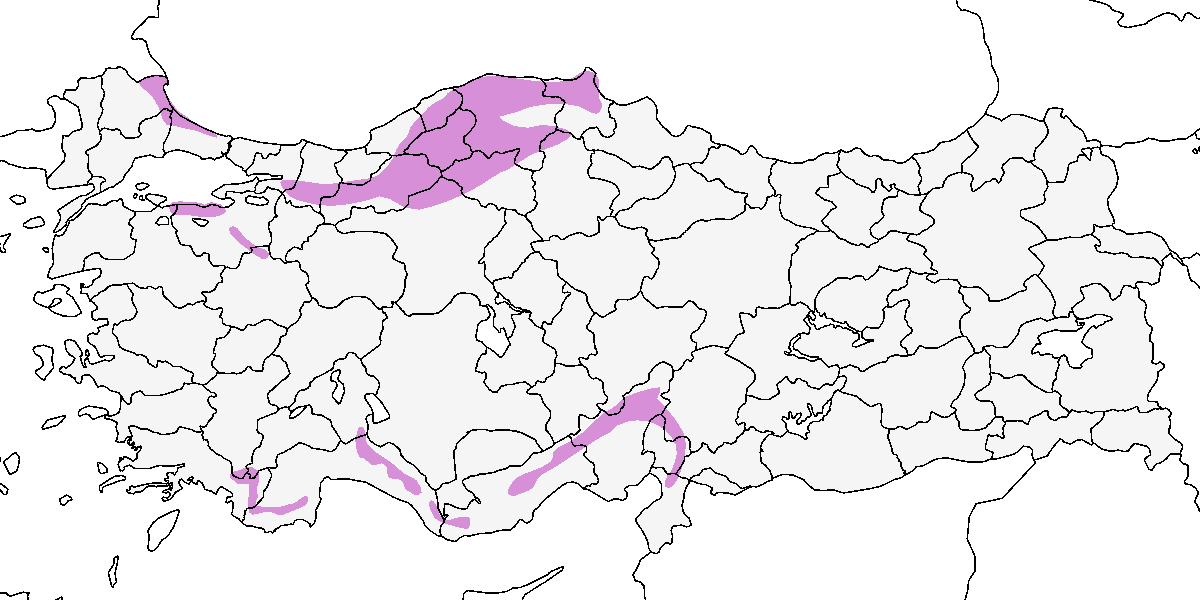
\includegraphics[keepaspectratio]{images/harita_Dendrocopos leucotos.png}}

\textbf{Üreme}

\textbf{Yuvalama alanı:} Eski ve yaşlı ormanlarda, subasar ormanlarda
yuvalar. Deniz seviyesinden 1500 metreye kadar çıkar.\\
\textbf{Yuvası:} Türkiye'de yuva kaydı bulunmamaktadır.\\
\textbf{Yumurta sayısı:} Türkiye'de yumurta sayısı bilinmemektedir.\\
\textbf{Üreme dönemi:} Mayıs ve haziran aylarında çiftler halinde
gözlenmiştir.

\textbf{Alttürler ve Sınıflandırma}

Türkiye'de bulunan \emph{lilfordi} alttürü, nominat \emph{leucotos}'tan
belirgin şekilde ayrılır. Sırt bölgesi tamamen beyaz değil, siyah-beyaz
çizgilidir. Alın, göz pınarı, kulak örtü tüyleri ve çene bölgesi
belirgin şekilde sarımsı renktedir. Kulak örtülerinin arkasından enseye
uzanan siyah çizgi dikkat çekicidir. Gıdı çizgisi daha kalındır; böğür,
göğüs yanları ve karın bölgesinde daha geniş siyah çizgiler bulunur.
Kuyruk sokumu siyahtır ve beyazlık yalnızca tüy uçlarında yer alır. Omuz
tüyeleri daha uzundur. Kanat telekleri, örtüleri ve kın telekleri eşit
kalınlıkta ve düzensiz şekilde siyah-beyaz çizgilidir; bu çizgilenme
kalın siyah ve ince beyaz şeritler şeklinde değildir. Alt kısımların
zemin rengi sarımsıdır; \emph{leucotos}'ta bu renk daha soluk, krem
tonundadır.

\section{Orman Alaca
Ağaçkakanı}\label{orman-alaca-aux11fauxe7kakanux131}

\emph{Dendrocopos major}, Great Spotted Woodpecker

\textbf{\emph{Nispeten yaygın olarak yer yer çok sayıda bulunan
yerlidir.}}

Dağlık ibreli ormanlarda yaygındır ancak genellikle az sayıda bulunur.
En bol olduğu bölgeler Karadeniz ve Marmara'dır. Genellikle 1000
metrenin üzerinde görülür, ancak Doğu Karadeniz'de 300 metreden itibaren
kaydedilmiştir. Bitlis'e kadar uzanır (Berk, Cronau \& Have, 1993).
Marmara ve Trakya'da muhtemelen deniz seviyesine kadar iner, ancak bu
bölgelerde yaz sonu ve sonbaharda kaydedilen bireyler, alaca ağaçkakan
ile aynı alanlarda gözlendiği için üreme sonrası dağılımı yansıtıyor
olabilir.

\pandocbounded{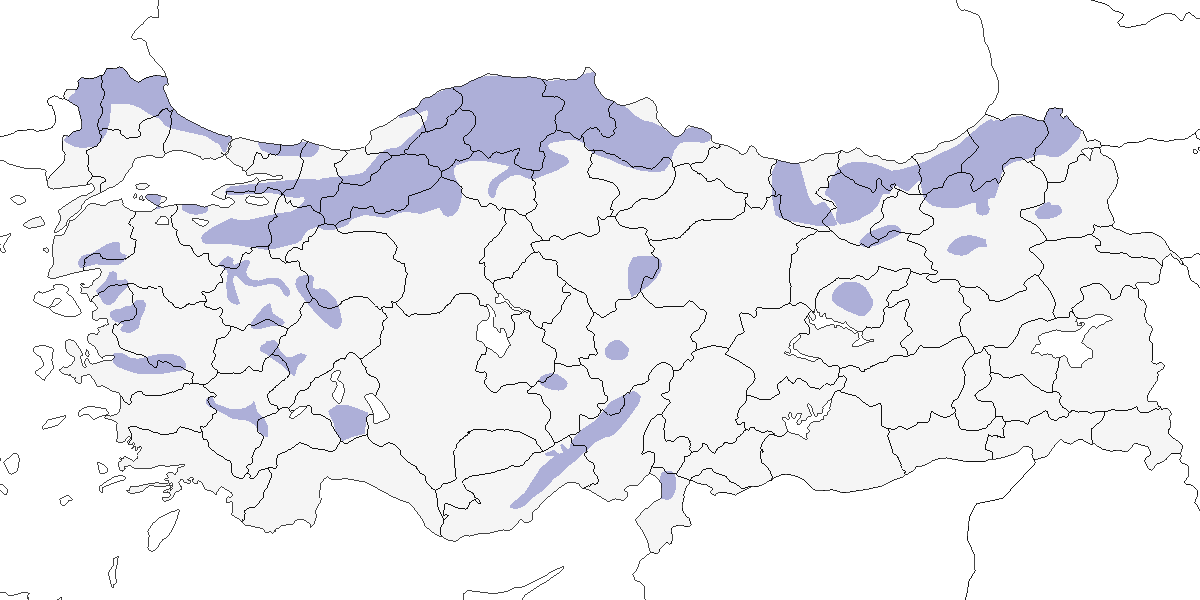
\includegraphics[keepaspectratio]{images/harita_Dendrocopos major.png}}

\textbf{Üreme}

\textbf{Yuvalama alanı:} Çoğunlukla dağlık, ibreli ormanlarda yuvalar.\\
\textbf{Yuvası:} Ağaçlarda, kuşların açtığı deliklere yuva yapar ve
yumurtalarını hiçbir malzeme koymadan deliğin tabanına bırakır.\\
\textbf{Yumurta sayısı:} Türkiye'de yumurta sayısı bilinmemektedir.
Diğer yerlerde olağan kuluçka büyüklüğü 4--7 yumurtadır.\\
\textbf{Üreme dönemi:} Nisan ayında yumurtlar. Yavrular mayıs ortasından
itibaren yumurtadan çıkar ve haziran başında yuvada görülür.
\textbf{MAR:} 3 Haziran 2002'de Uludağ'da bir delikte yavrularını
besleyen erişkinler gözlenmiştir. 7 Haziran 1988'de yine Uludağ'da, 1400
metrede üreme teyit edilmiştir (Jetz, 1995). 4 Haziran 1996'da Belgrad
Ormanı'nda, yumurtlamanın nisan sonunda olduğunu gösterecek şekilde
tüylenmiş yavrular gözlenmiştir. \textbf{KAR:} 17 Haziran 1975'te Torul
yakınlarında yiyecek taşıyan bir erişkin, 21 Temmuz 1996'da İspir'de
genç bir birey, 7 Ağustos 1992'de Şavşat'ta bir aile grubu ve 14 Haziran
2004'te Sivrikaya'da yumurtlamanın 8 Mayıs civarında olduğunu gösterecek
şekilde güçlükle uçabilen, yeni tüylenmiş bir yavru gözlenmiştir.
\textbf{İÇA:} 17 Mart 1984'te Kızılcahamam'da 15'ten fazla bireyin
öttüğü duyulmuş (Barış \emph{vd.}, 1984). 19 Nisan 1996'da üreyen bir
çift, 22 Mayıs 1996'da bir telefon direğinde ve yakınlarında iki yuva ve
23 Mayıs 2006'da bir çam ağacında 1,5 m yüksekte, içinde birkaç yavru
bulunan bir yuva kaydedilmiştir.

\textbf{Alttürler ve Sınıflandırma}

Türkiye'ye endemik olan \emph{paphlagoniae} alttürü bulunur. Bu alttür,
Winkler ve Christie tarafından İngiltere'den Kafkaslar'a kadar yayılan
\emph{pinetorum} alttürüne dahil edilmiştir (Vaurie, 1959b) (Hoyo
\emph{vd.}, 2002).

\section{Alaca Ağaçkakan}\label{alaca-aux11fauxe7kakan}

\emph{Dendrocoptes syriacus}, Syrian Woodpecker

\textbf{\emph{Yaygın olaral ve çok sayıda bulunan bir yerlidir.}}

Alçak ve orta yüksekliklerde en yaygın ağaçkakan türüdür. Meyve
bahçeleri, zeytinlikler, seyrek ağaçlı tarım alanları ve yerleşim
çevresindeki kavaklıklar gibi açık alanlarda bulunur. Alçak rakımlarda
yalnızca ibreli ormanlarda görülse de her tür ağaçlık alanda üreyebilir.
Deniz seviyesinden, kuzey ve batıda 2100 metreye kadar kaydedilmiştir.
Toroslar'da, orman ağaçkakanı ile daha geniş ölçüde örtüştüğü için
nadiren 900 metrenin üzerine çıkar. Genellikle 1000--2000 metre
arasında, çoğunlukla bu aralığın alt sınırında orman ağaçkakanı ile yer
değiştirir. Görünüşe göre güneybatı Ege ve muhtemelen kuzey Trakya'nın
bazı bölümlerinde ortanca ağaçkakan ile de yer değiştirir. Istranca
Dağları'nın Bulgaristan tarafında neredeyse tamamen orman ağaçkakanı ile
yer değiştirmiştir (Milchev, 1994). Nisan--Mayıs 1993'te yapılan yoğun
arazi çalışmasına rağmen Rize Çamlıhemşin'de hiç kaydedilmemiştir
(Faldborg, 1994).

\pandocbounded{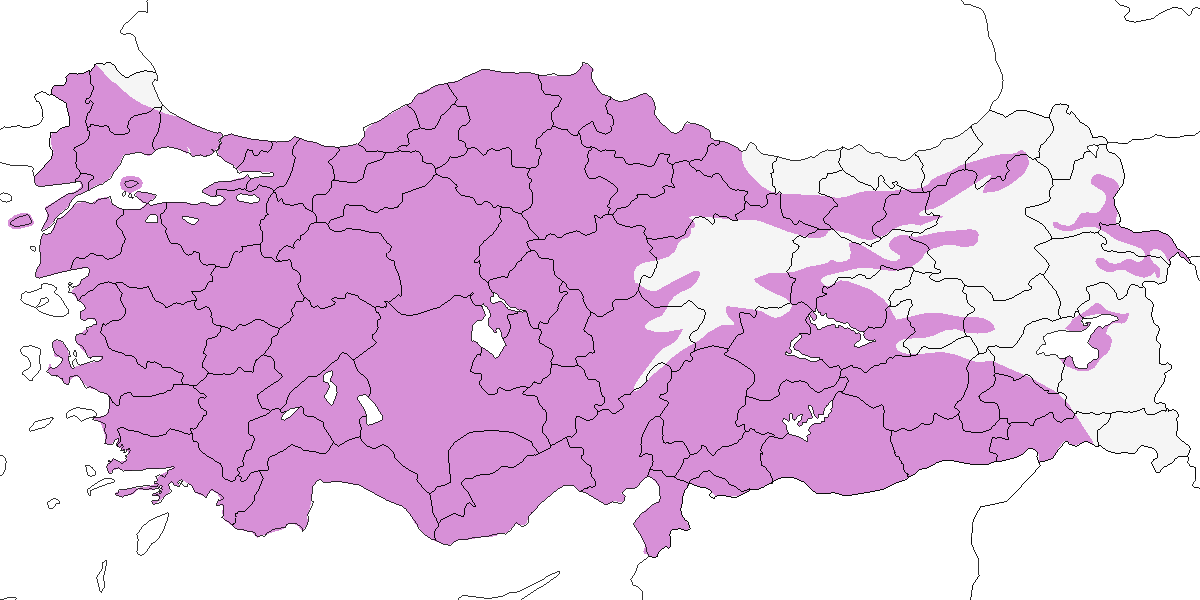
\includegraphics[keepaspectratio]{images/harita_Dendrocopos syriacus.png}}

\textbf{Üreme}

\textbf{Yuvalama alanı:} Meyve bahçeleri, zeytinlikler, açık ağaçlık
alanlar, seyrek ağaçların ya da baltalıkların bulunduğu tarım alanları
ve açık arazilerde yuva yapar.\\
\textbf{Yuvası:} Ağaç gövdelerine ya da dallarına açılmış, kaplanmamış
yuva bölmelerine ulaşan deliklerde yuvalar. Birecik'te antepfıstığı
bahçelerinde daha kalın gövdeli ağaçları tercih eder ve yuvalar
genellikle 2 metreden, hatta bazıları 1 metreden daha aşağıda bulunur.
Diğer habitatlarda yuva delikleri 10 metreye kadar yüksekte olabilir.
Materyal kullanılmaz; sadece doğal oyuk ya da ağaçkakanın açtığı delik
şeklindedir. Alaca ağaçkakanın oyduğu yuva delikleri, sonraki yıllarda
sığırcık ve sarı boğazlı serçe gibi türler tarafından da kullanılmakta
olup, bu türler yuva alanı açısından kısmen bu ağaçkakan türüne
bağımlıdır.\\
\textbf{Yumurta sayısı:} Türkiye'de gözlenen yumurta sayısı bir yuvada
2, bir yuvada 5'tir. Bir yuvada 1, bir yuvada 2, bir yuvada 4 ve bir
yuvada 5 yavru sayılmıştır. Türkiye'deki çok az sayıda yuva yakından
incelenmiştir ve bu sınırlı veri durumu tam yansıtmayabilir. Başka
yerlerde genellikle 5-7 yumurta bırakır.\\
\textbf{Üreme dönemi:} Yumurtlama genellikle nisan sonunda başlar.
Yavrular haziran sonunda ve temmuz ayında yuvadan çıkar. \textbf{MAR:}
18 Haziran 1973'te Belgrad Ormanı'nda tüylenmiş yavrusuyla bir erişkin
ve 23 Haziran 1973'te Keşan yakınlarındaki yuvasına yiyecek taşıyan bir
erişkin görülmüştür. 31 Mayıs 1988'de Truva'daki bir yuvada büyük bir
yavru kaydedilmiş, bu da yumurtlamanın nisan sonunda gerçekleştiğini
göstermektedir. \textbf{EGE:} 7 Mayıs'tan itibaren erişkinler yuva
deliklerinde gözlenmiş, 2 Haziran 1974'te Kuşadası'nda içinde tamamen
gelişmiş yavru olan bir yuva bulunmuştur. Bu durum yumurtlamanın nisan
sonunda gerçekleştiğini gösterir. \textbf{AKD:} 15 Haziran 1992'de
Taşucu yakınlarında bir yuvada iki yumurta, 9 Haziran 1993'te
Uzuncaburç'taki bir yuvada büyük bir yavru gözlenmiştir. 7 Mayıs 2004'te
Uzuncaburç yakınlarındaki üç yuvanın yumurtlamaya hazır ancak boş olduğu
kaydedilmiştir. \textbf{KAR:} 27 Mayıs 1992'de Kızılırmak Deltası'nda
yiyecek isteyen yavruların bulunduğu ilk yuvalar bulunmuştur (Hustings
\& Dijk, 1994). \textbf{İÇA:} 27 Mayıs 1993'te Hasan Dağı'nda yuva
yapımı gözlenmiştir. Bu geç tarih, muhtemelen başarısız bir girişim
sonrası yapılan ikinci kuluçkadır. \textbf{GDA:} Birecik'te mayıs sonu
ve haziran başında büyük veya tamamen gelişmiş 5 yavru kaydedilmiş, bu
da yumurtlamanın nisan sonunda olduğunu göstermektedir. Durnalık'ta bir
yuvada 9 Mayıs 2004'te beş yumurta, 16 Mayıs 2004'te yeni çıkmış
yavrular; başka bir yuvada ise 9 Mayıs'ta yumurtalar ve 23 Mayıs'ta
küçük yavrular gözlenmiştir.

\textbf{Alttürler ve Sınıflandırma}

Türkiye'de nominat alttürü bulunur.

\section{Küçük Ağaçkakan}\label{kuxfcuxe7uxfck-aux11fauxe7kakan}

\emph{Dryobates minor}, Lesser Spotted Woodpecker

\textbf{\emph{Yaygın olarak ve nispeten çok sayıda bulunan yerlidir.}}

Çoğunlukla alçak bölgelerde, nispeten az sayıda bulunur. Sulakalanlarda
daha yüksek yoğunlukta görülür. Kocaçay Deltası'nda 200 çiftten fazla
birey bulunabilir (Ertan, 1996). Nisan 1992'de Kızılırmak Deltası'nda
75--125 çift olduğu tahmin edilmiştir (Hustings \& Dijk, 1994). Mayıs
1993'te Rize Çamlıhemşin çevresindeki düşük rakımlarda bol sayıda üreyen
bir tür olarak tanımlanmıştır (Faldborg, 1994). Doğu Anadolu'da
genellikle yaprak döken, bazen karışık ormanlarda ve meyve bahçelerinde
görülür. Güneydoğu Anadolu'da yakın zamanda Diyarbakır çevresinde
(Karakaş \& Kılıç, 2002) ve daha önce Siirt'in güneyindeki dağlık
bölgede kaydedilmiştir (Goriup \& Parr, 1983). Alçak ve orta
yüksekliklerde bulunduğu bilinmektedir, ancak yükseklik sınırı kesin
değildir. Türkiye'de 1000 metrenin üzerinde nadiren kaydedilmiştir.
Ermenistan ve Kafkaslar'da ise 2000 metreye kadar çıkar (Kumerloeve,
1961).

\pandocbounded{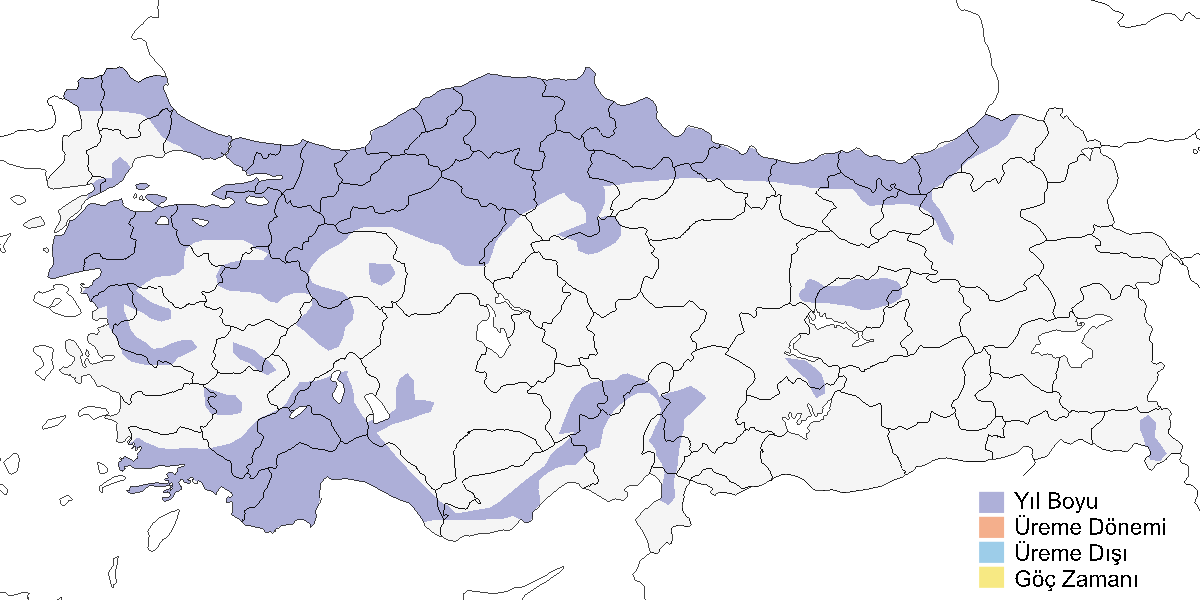
\includegraphics[keepaspectratio]{images/harita_Dryobates minor.png}}

\textbf{Üreme}

\textbf{Yuvalama alanı:} Ormanlarda, daha küçük ağaçlık alanlarda ve
ağaç sıralarında yuva yapar.\\
\textbf{Yuvası:} Yuvasını ağaç gövdelerinde oyuklara yapar. Dişbudak
(\emph{Fraxinus excelsior}) gibi ağaçlarda tercih ettiği gözlenmiştir.\\
\textbf{Yumurta sayısı:} Türkiye'de yumurta sayısı bilinmemektedir.
Diğer bölgelerde genellikle 4-6 yumurta bırakır.\\
\textbf{Üreme dönemi:} Muhtemelen nisanda yumurta koyar. Yavrular mayıs
sonunda yumurtadan çıkar, haziran ortasından itibaren yuvayı terk eder.
\textbf{MAR:} Kocaçay Deltası'nda, orman ve subasar alanlar arasındaki
geçiş zonlarında ürediği belirlenmiştir. 31 hektarlık alanda 6 yuva
kaydedilmiş ve hektar başına 0,29 çiftin ürediği hesaplanmıştır.
Haziranın ikinci haftasında yeni tüylenmiş bir yavru ve 16 Mayıs 1966'da
bir yuva deliğinde erişkin kaydedilmiştir (Ertan, 1996). 22 Temmuz
1966'da Çamlıca Tepeleri'nde bir erişkinle birlikte genç bir birey, 4
Haziran 1996'da ise Belgrad Ormanları'nda yuva deliğinde bir erişkin
gözlenmiştir. \textbf{AKD:} 20 Nisan--25 Mayıs 1989'da Dalyan bölgesinde
kullanılan iki yuva tespit edilmiştir. 14 Mayıs 2001'de Akseki'de bir
çift, 26 Mayıs 2005'te ise aynı yerde bir meşe kütüğündeki oyukta dişi
birey gözlenmiş, yuvada en az iki yavrunun bulunduğu tahmin edilmiştir.
\textbf{KAR:} Kızılırmak Deltası'nda 9 Mayıs 1977'de bir yuva deliği
bulunmuş, haziran ayında yuvadan uçmuş birkaç yavru kaydedilmiştir. 10
Haziran 1975'te bir aile grubu gözlenmiş ve yumurtlamanın mayıs başında
gerçekleştiği düşünülmüştür (Dijksen \& Kasparek, 1985). 1992'de
yavruların yiyecek isteme ötüşleri 27 Mayıs'ta duyulmuş, yuvadan uçmuş
yavrular ise haziranın ikinci haftasında gözlenmiştir (Hustings \& Dijk,
1994).

\textbf{Alttürler ve Sınıflandırma}

Türkiye'de alt kısımları koyu renkli olan ve bazen kahverengimsi tonlar
gösteren, ayrıca tepenin arkasından kulak örtülerinin arkasına kadar
uzanan siyah banda sahip \emph{danfordi} alttürü bulunur.

\section{Küçük Yeşil
Ağaçkakan}\label{kuxfcuxe7uxfck-yeux15fil-aux11fauxe7kakan}

\emph{Picus canus}, Grey-headed Woodpecker

\textbf{\emph{Lokal olarak nispeten az sayıda sayıda bulunan yerlidir.}}

Yoğun olarak Batı Karadeniz ve Trakya'da bulunur. Deniz seviyesinden
2300 metrenin üzerine kadar kaydedilmiştir. Özellikle Trakya'da karışık
ormanlarda da gözlenmiş olsa da çoğu kayıt ibreli ormanlardandır. Doğu
Karadeniz ormanlarında, 1993'te Çamlıhemşin yakınlarında ürediği
kanıtlanmıştır (Faldborg, 1994). Ayrıca İkizdere (Heiser, 1984) ve Ayder
(Berg, 1988) çevresinde kaydedilmiştir. Çamlıhemşin çevresinde, ağaç
sınırının yaklaşık 300--400 metre altına kadar oldukça bol olduğu
düşünülmektedir. Akdeniz Bölgesi'nde ise 1989'dan bu yana Akseki'de az
sayıda ancak sık gözlenmektedir. Orta ve Doğu Toroslar'ın eteklerinde,
Mersin Uzuncaburç'un yukarı kesimlerinde de kaydedilmiştir (Kirwan \&
Martins, 2000).

(Krüper, 1875) ve (Mathey-Dupraz, 1920--24), 1850--1900 yılları arasında
İstanbul Boğazı civarında bulunduğunu belirtmiş ve bu bölgeden en az bir
tahnit örneği alınmıştır (Kirwan, 1997). Şubat 1910'da İstanbul'dan iki
örnek, Ağustos 1934'te Bolu Mengen yakınlarından üç, Ekim 1934'te
Bolu'dan bir ve 15 Mayıs 1949'da İstanbul Büyükdere'den bir örnek
toplanmıştır. Ancak bunların Bulgaristan'dan geldiği düşünülmüştür
(Kumerloeve, 1961). Nisan 1969'da İstanbul Belgrad Ormanları, 12 Mayıs
1967'de Kırklareli Demirköy, 29 Nisan 1972'de Ankara Kızılcahamam ve 31
Ocak 1917'de Kırklareli Mandra yakınlarında kaydedilen bireylerin de
hatalı değerlendirildiği anlaşılmıştır. Bu nedenle Türkiye'deki varlığı
uzun süre şüpheli kabul edilmiştir (Berg, 1988). Sonrasında kuzeybatı
bölgelerdeki varlığı doğrulanmış ve Adana Pozantı'da 18 Haziran 1964,
Mersin Gülek'te 13 Nisan 1965, Zigana Geçidi'nde 30--31 Ağustos 1971
tarihlerindeki kayıtlar daha güvenilir bulunmuştur. 1988--1990
yıllarında Istranca Dağları'nın Bulgaristan tarafında yapılan
çalışmalarda, 5 kilometrelik karelerin \%35'inde bu türün bulunduğu
tespit edilmiştir (Milchev, 1994).

\pandocbounded{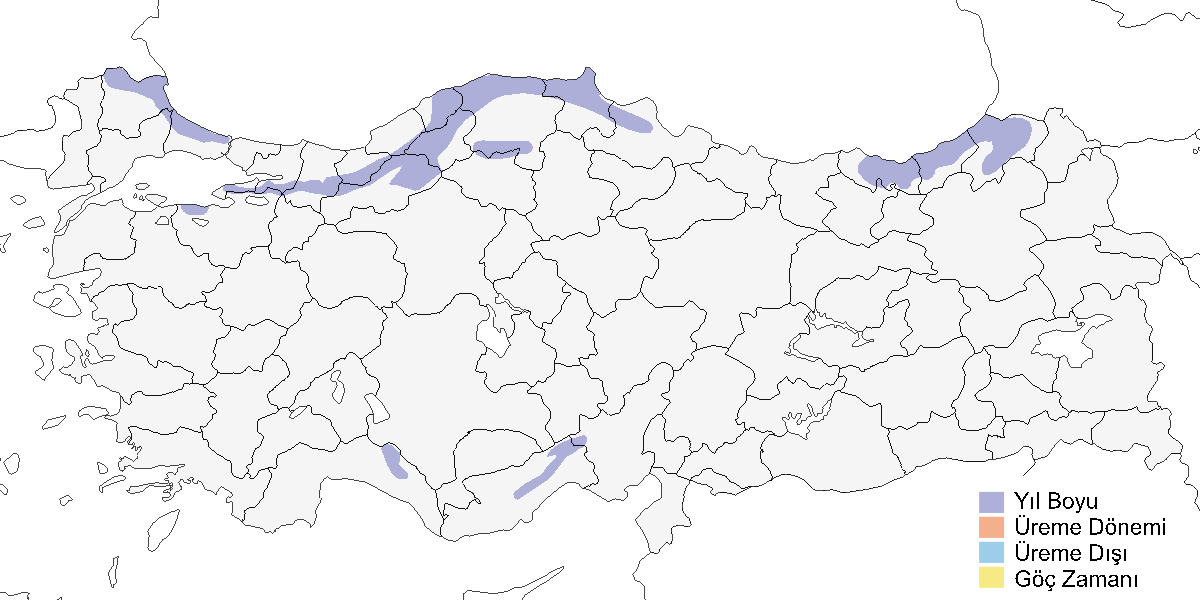
\includegraphics[keepaspectratio]{images/harita_Picus canus.png}}

\textbf{Üreme}

\textbf{Yuvalama alanı:} Trakya ve Karadeniz bölgesinde yaşlı kayın
ormanlarında bulunur. Akdeniz bölgesinde özellikle açık çam ormanlarında
gözlenmiştir.\\
\textbf{Yuvası:} Bilinen yuvaları yaşlı kayın ağaçlarında yuvalar.\\
\textbf{Yumurta sayısı:} Türkiye'de yumurta sayısı bilinmemektedir.
Diğer ülkelerde olağan yumurta sayısı 4-5'tir.\\
\textbf{Üreme dönemi:} Yumurtlama nisan ortasında başlar, yavrular
haziran başında çıkar. \textbf{KAR:} Çamlıhemşin-Ardeşen bölgesinde
yaygın olarak üremektedir ve neredeyse her gün duyulmaktadır. 3 Mayıs
1993'te Çamlıhemşin-Ardeşen arasında, yaklaşık 37-40 metre uzunluğundaki
bir kayın (\emph{Fagus orientalis}) ağacının 27 metre yüksekliğinde bir
yuvada iki erişkinin 3-4 saatlik vardiyalarla kuluçkaya yattığı
gözlenmiştir. 8 Haziran'da ise erişkinlerin sık sık yuvayı ziyaret
etmesi, yumurtaların çatladığını göstermiştir (Faldborg, 1994).
\textbf{AKD:} Akseki çevresindeki açık çam ormanlarında nisan ve haziran
ayları arasında gözlenmiştir.

\textbf{Alttürler ve Sınıflandırma}

Türkiye'de nominat alttürü bulunur.

\section{Yeşil Ağaçkakan}\label{yeux15fil-aux11fauxe7kakan}

\emph{Picus viridis}, European Green Woodpecker

\textbf{\emph{Yaygın olarak ve yer yer çok sayıda bulunan yerlidir.}}

Ülkenin büyük bölümünde, hem yaprak döken hem de muhtemelen daha sık
olarak ibreli ormanlarda, nispeten lokal bir yerli türdür. Genellikle
700 ile 1900 metre arasında görülür. Ancak Doğu Karadeniz Dağları'nda ve
Toroslar'da ara sıra 2200 metreye kadar çıktığı kaydedilmiştir. Bazı
bölgelerde kayıtların gösterdiğinden daha bol olabilir. Nitekim Istranca
Dağları'nın Bulgaristan tarafında yapılan bir araştırmada, sayım yapılan
5 kilometrelik karelerin \%91'inde bu türe rastlanmıştır (Milchev,
1994).

Sonbaharda Van Gölü Havzası'ndan iki kayıt vardır {[}Ven \& Gheyselinck
(1980); L. J. Dijksen ve L. C. van Beckhoven{]}. Güneydoğu Anadolu'da
ise doğuda Siirt'e kadar üç kez kaydedilmiştir.

\pandocbounded{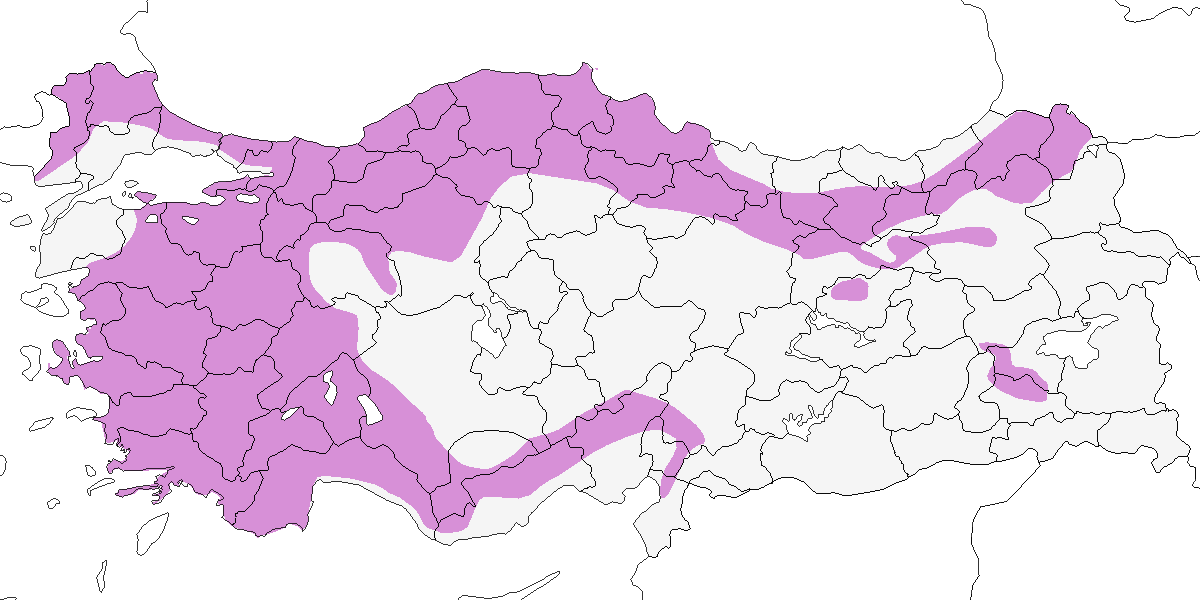
\includegraphics[keepaspectratio]{images/harita_Picus viridis.png}}

\textbf{Üreme}

\textbf{Yuvalama alanı:} Yaprak döken ve ibreli ormanlarda ürer.\\
\textbf{Yuvası:} Ağaçlara açtığı kovuklarda yuvalar.\\
\textbf{Yumurta sayısı:} Türkiye'den veri yoktur. Türkiye dışındaki
gözlemlere göre olağan yumurta sayısı 5-7'dir.\\
\textbf{Üreme dönemi:} İlk yumurtalar nisan ayında bırakılır, yavrular
haziran sonu ve temmuzda yuvadan çıkar. \textbf{MAR:} 1993 yılında
Kocaçay Deltası'nda yapılan çalışmada 31 hektarlık alanda hektar başına
0-29 çiftin ürediği tahmin edilmiştir. 19 Mayıs 1967'de bir yuvada,
yavruların yuvanın girişinde beslendiği gözlenmiştir. Bu gözlem,
yavruların büyük olduğunu ve ilk yumurtanın 10 Nisan civarında
bırakıldığını göstermektedir (Ertan, 1996). \textbf{EGE:} Temmuz 1966'da
genç bireyler erişkinlerle birlikte gözlenmiştir. 1 Haziran 1995'te
Marmaris yakınlarında genç bir birey gözlenmiş olup bu kayıt
yumurtlamanın nisan ortasında gerçekleştiğini göstermektedir.
\textbf{AKD:} 15 Temmuz 2004'te Akseki'de genç bireyler kaydedilmiştir.
\textbf{KAR:} Kızılırmak Deltası'nda temmuz 1971'de iki yavrulu bir çift
ve tek yavrulu iki çift gözlenmiştir (Dijksen \& Kasparek, 1985).
\textbf{İÇA:} 9 Temmuz 1968'de Porsuk'ta bir aile grubu gözlenmiş, örnek
olarak bir genç alınmıştır (Rokitansky \& Schifter, 1971).

\textbf{Alttürler ve Sınıflandırma}

Nominat alttürden biraz daha küçük, soluk ve daha az sarı olan karelini
alttürü görülür. İran ve Irak'ta yaşayan ve Siirt ile Şırnak'ta
bulunması muhtemel olan \emph{innominatus} alttürünün ise genetik
verilere dayanarak ayrı bir tür olabileceği öne sürülmüştür (Perktas,
Barrowclough \& Groth, 2011). Ancak bu alttür ile \emph{karelini}
arasındaki tüy örtüsü farkları yalnızca ince renk tonlarıyla sınırlıdır.

\section{Kara Ağaçkakan}\label{kara-aux11fauxe7kakan}

\emph{Dryocopus martius}, Black Woodpecker

\textbf{\emph{Yaygın olarak nispeten az sayıda bulunan yerlidir.}}

En çok Doğu Karadeniz'de Sümela ve Borçka'da, batıda ise düzenli olarak
Uludağ, Yalova, Yenice Ormanları, Ilgaz Dağları ve çevresinde
kaydedilmiştir. Ülkenin kuzey kesimlerinde genellikle 900 metreden
başlayarak en az 2000 metreye kadar görülür. Kocaçay Deltası (Ertan,
1996) ve Trakya'da deniz seviyesine kadar indiği de bilinmektedir.
1988--1990 yıllarında Bulgaristan'da gerçekleştirilen üreyen kuş
sayımlarında, 5 kilometrelik karelerin \%28'inde kaydedilmiştir
(Milchev, 1994). Toroslar'daki durumu belirsizdir. Yayılışın orta
kesimlerinde ``nadir ama ara sıra gözlenen'' bir tür olarak
tanımlanmıştır (Danford, 1877-78). Ancak bu tarihten sonra çok az
gözlemci tarafından kaydedilmiştir. Bölgedeki en yeni kayıtlar 1993 ve
1998 yıllarında Gidengelmez Dağları'ndan bildirilmiştir. Mayıs 2008'de
ise Osmaniye'nin güneyindeki Zorkun Yaylası'nda, 700 metrede bulunan bir
çam ormanında tespit edilmiştir.

Kışın üreme alanının dışına ulaşır, Ankara Kazan'da ve Hacettepe
Üniversitesi'indeki kayıtları üreme sonrası dağılmaya işaret eder.

\pandocbounded{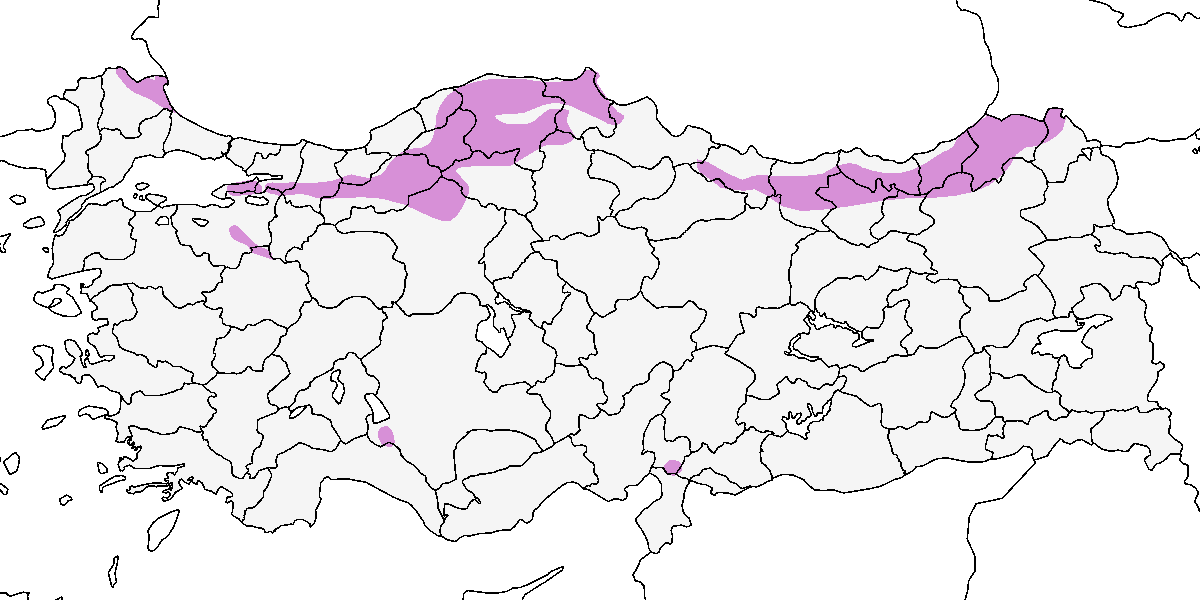
\includegraphics[keepaspectratio]{images/harita_Dryocopus martius.png}}

\textbf{Üreme}

\textbf{Yuvalama alanı:} Genellikle yaşlı ormanlarda bulunur.\\
\textbf{Yuvası:} Türkiye'de dışında yaşlı ibreli ve yapraklı ağaçlarda
yuva yaptığı bilinir.\\
\textbf{Yumurta sayısı:} Türkiye'de bilinmemektedir.\\
\textbf{Üreme dönemi:} Türkiye'de bilinmemektedir.

\textbf{Alttürler ve Sınıflandırma}

Türkiye'de nominat alttürü bulunur.

\section{Küçük Kerkenez}\label{kuxfcuxe7uxfck-kerkenez}

\emph{Falco naumanni}, Lesser Kestrel

\textbf{\emph{Yaygın olarak ve nispeten çok sayıda bulunan yaz
konuğudur.}}

Popülasyonun büyük bölümünü barındıran İç Anadolu'da tür, genellikle
kasaba, köy ve harabelerde ya da kuru, ağaçsız tarım alanları ile
yerleşime kapalı bölgelerde küçük koloniler halinde ürer. Koloniler
genellikle 3-5 çiftten oluşur, ancak bazı bölgelerde 20 çiftin üzerine
çıkabilir. Tercih ettiği habitatlar çoğunlukla hububat tarlalarının
baskın olduğu alanlar ile kuru ve sulak çayırlar, bataklıklar ve bazen
yerleşimlere yakın kaya yüzleridir. Bazı koloniler 2600 metre, hatta
3000 metreyi aşan yüksekliklerde bulunur. Orta Anadolu'da rastgele
seçilmiş 10 kilometrekarelik 60 alanda yapılan araştırmada, 11 Nisan--15
Mayıs tarihleri arasında 231 yerleşim yeri ziyaret edilmiştir (Parr
\emph{vd.}, 1995). Bu çalışmaya göre İç Anadolu'daki toplam popülasyonun
1500--3500 çift arasında olduğu tahmin edilmiştir (Biber, 1990). Bu,
İspanya'dan sonra dünyanın en büyük ikinci popülasyonunun Türkiye'de
olduğunu göstermektedir.

Üreme sonrası dönemde temmuz sonu ve ağustos ayında İç Anadolu'daki
toplanma alanlarında 100'den fazla birey kaydedilir. Mogan Gölü gibi
bazı alanlarda bu sayı daha da artar. Burada ağustos sonu ile ekim başı
arasında 300'ün üzerinde birey düzenli olarak görülmektedir.

İlkbahar göçü mart ortasında başlasa da nisan ortasına kadar
yaygınlaşmaz. Buna karşın, 3 Nisan 2004'te Kozanlı Saz Gölü'nde 100
birey kaydedilmiştir. İlkbahar geçişi en azından mayıs ortasına kadar
sürer. Sonbahar göçü ise eylül sonunda en yoğun dönemine ulaşır, ancak
bazı bireyler ekim sonuna kadar bölgede kalabilir. Temmuz sonu ile ekim
başı arasında Türkiye'deki üç önemli göç izleme alanında az sayılarda da
olsa düzenli olarak görülür. Türkiye'nin güneyi ve batısındaki bazı
alanlarda kışladığına dair güçlü kanıtlar vardır. 27 Kasım 1970'te
Akdeniz kıyısında 13 birey kaydedilmiş, 1969'un kasım sonu--aralık
başında ise üç lokalitede toplam 18 birey gözlenmiştir. En son kış
kayıtları ise Gediz Deltası'ndandır ve burada yalnızca küçük sayılarda
bireyler görülmüştür.

Türün Marmara, Ege ve Akdeniz bölgeleri ile Kuzey Anadolu'daki
popülasyonları muhtemelen azalmaktadır. Bu bölgelerdeki kolonilerin bir
kısmı son 10--30 yıl içinde ortadan kalkmıştır. Buna karşın İç ve Doğu
Anadolu'da hâlâ yaygın ve bol olarak üremektedir.

\pandocbounded{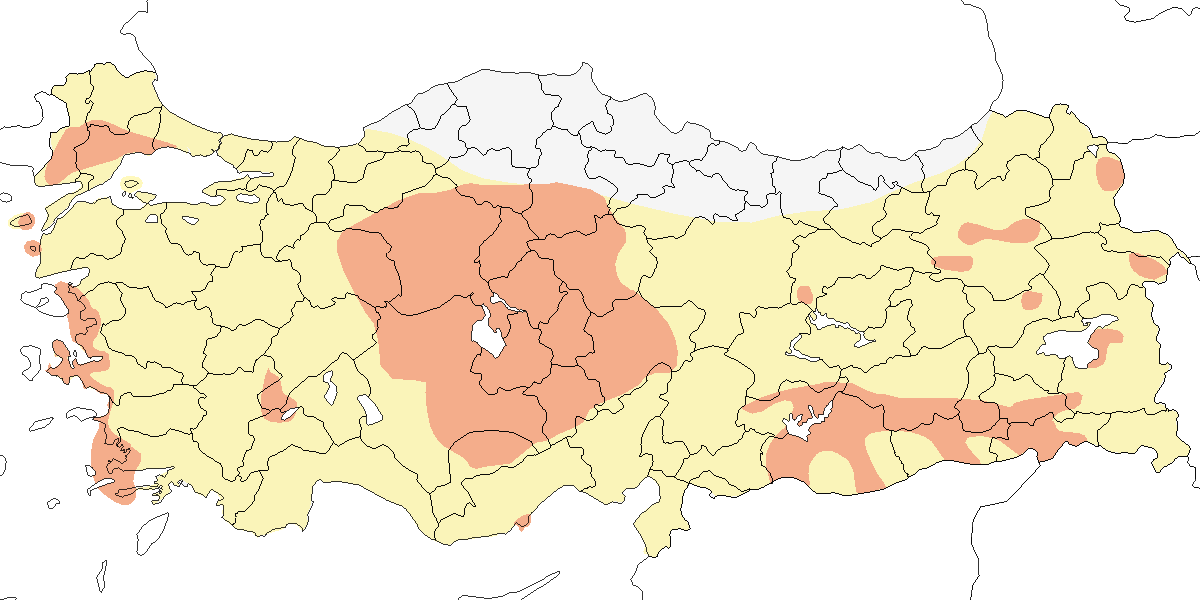
\includegraphics[keepaspectratio]{images/harita_Falco naumanni.png}}

\textbf{Üreme}

\textbf{Yuvalama alanı:} Köylerde ya da çevresi tarla, çayır veya
bataklıklarla çevrili izole binalarda yuvalar. Ayrıca duvarlardaki
yarıklar, harabeler, taşlar ve kayalıklardaki oyuklar da yuvalama alanı
olarak kullanılır. Kolonilerde genellikle 2-30 çift bulunur. Bir çatıda
sekizden fazla yuva bulunabilir (Wadley, 1951).\\
\textbf{Yuvası:} Çoğunlukla çatı kiremitlerinin, özellikle de çatı sırt
kiremitlerinin altına yapılır. Yuva, içinde materyal olmayan, hafif
kazınmış bir oyuktur.\\
\textbf{Yumurta sayısı:} Türkiye'de gözlenen yumurta sayısı 4 yumurta (1
yuvada) ve 5 yumurta (1 yuvada) olarak kaydedilmiştir. Bir yuvada 2
yavru, bir yuvada 3 yavru, iki yuvada 4 yavru ve iki yuvada 5 yavru
kaydedilmiştir.\\
\textbf{Üreme dönemi:} Erişkinler mart sonu ve nisan başında üreme
alanlarına döner. Yumurtlama nisan ortasında başlar. Yavrular haziran
ortasından itibaren uçmaya başlar. \textbf{MAR:} 14 Haziran 1966'da
Susurluk'ta uçmaya başlayan bir yavru, yumurtlamanın nisan ortasında
gerçekleştiğini göstermektedir. \textbf{EGE:} 23-29 Nisan 2003'te
Akköy'deki bir yuva deliğinde bir dişi ve erkek birey görülmüş ancak
yumurtlama gerçekleşmemiştir. İzmir'de 3 Mayıs 1967'de bir erkek birey,
iki dişiyle çiftleşmiştir. 13-15 Mayıs 1899'da iki kolonide çok sayıda
yumurta görülmüş ancak 8-11 Mayıs 1899'da diğer iki kolonide henüz
yumurtlama gerçekleşmemiştir (Selous, 1900). 12 Mayıs 1980'de Bafa
Gölü'nde içinde bir yumurta bulunan tamamlanmamış bir kuluçka
kaydedilmiştir (Kasparek, 1988). 12 Mayıs 1970'te Milet'te içinde 5
yavru bulunan bir yuva, yumurtlamanın nisan ortasında gerçekleştiğini
göstermektedir. \textbf{AKD:} 4 Mayıs 1951'de çiftleşme gözlenmiş
(Hollom, 1955) ve 5 Mayıs 1987'de Çukurova'da erişkinlerde kur davranışı
kaydedilmiştir. \textbf{İÇA:} 25 Mayıs 1975'te Sultansazlığı'nda biri 4,
biri 5 yumurtalı iki yuva ve 19 Haziran 1977'de 3 ve 5 yavrulu iki yuva
kaydedilmiştir (Kasparek, 1985). 17 Haziran 1977'de 4 yavruyla
kaydedilen bir yuva, yumurtlamanın mayıs başında gerçekleştiğini
göstermektedir (Pforr \& Limbrunner, 1982). 7 Temmuz 1907'de Konya
yakınlarında yavrulu birkaç yuva kaydedilmiştir. Yavrular genellikle
temmuz ortasında uçmaya başlar; en erken uçuş 19 Haziran 1996'dadır.
\textbf{DOA:} Van yakınlarında ve Nemrut Dağı çevresindeki köylerde
üreme döneminde erişkinler kaydedilmiş ancak yuva içerikleri hakkında
bilgi bulunmamaktadır. \textbf{GDA:} 5 Haziran 1935'te Gaziantep'te
içinde 4 yavru bulunan bir yuva (Bird, 1937) ve 22 Haziran 1982'de
Birecik yakınlarında içinde tüylenmiş yavru olan bir yuva
kaydedilmiştir.

\textbf{Alttürler ve Sınıflandırma}

Monotipik bir türdür.

\section{Kerkenez}\label{kerkenez}

\emph{Falco tinnunculus}, Common Kestrel

\textbf{\emph{Yaygın olarak nispeten çok sayıda bulunan yerlidir, kışın
göç alır.}}

Açık tarım alanları, bozkırlar, tepelik ve dağlık alanlar ile ormanlara
kadar, 4000 metreye varan yüksekliklerde farklı habitat tiplerinde
bulunur.

Göç geçişi Türkiye'nin doğu yarısında muhtemelen daha yoğundur. İstanbul
Boğazı ve Belen Geçidi'nde sadece küçük sayılarda birey kaydedilmiştir.
Bu gözlemler genellikle ağustos ortasından ekim başına kadar olan
dönemde yapılmıştır. Öte yandan, Borçka'da 11--25 Ekim 1977 tarihleri
arasında 450 birey sayılmıştır (Beaman, 1977). Ancak 1976 yılında yine
aynı bölgede, 17 Ağustos--10 Ekim arasında yalnızca 30 birey
gözlenmiştir. Bu farklılık, göçün en yoğun döneminin sonbaharın sonuna
denk geldiğini göstermektedir.

\pandocbounded{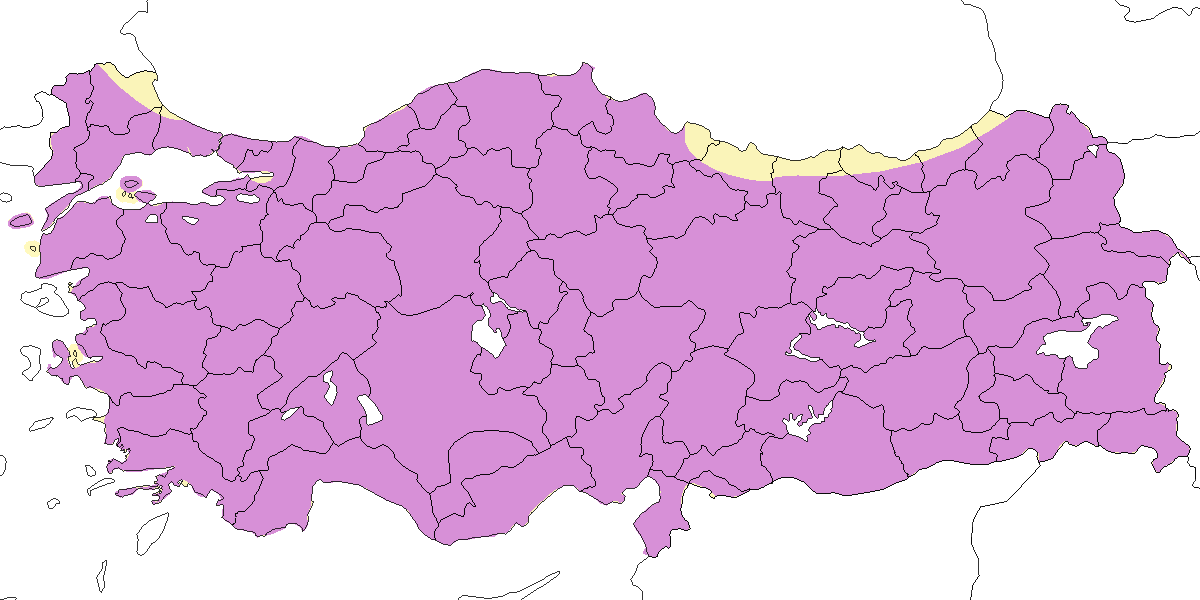
\includegraphics[keepaspectratio]{images/harita_Falco tinnunculus.png}}

\textbf{Üreme}

\textbf{Yuvalama alanı:} Sıklıkla seyrek ağaçlı açık tarım alanları,
ağaçlık çevreler, ağaçsız tepeler, vadili ve kayalıklı dağlık alanlar,
eski binalar, harabeler ve taş ocaklarında ürer.\\
\textbf{Yuvası:} Yarlarda, kaya oyuklarında veya insan yapımı yapılarda
yer alır. Genellikle başka türlerin eski yuvalarını kullanır. Yuvada
astar bulunmaz. Yuvalar, kaya yarıklarında, basamaklı yamaçlarda,
özellikle saksağan ve leş kargası gibi diğer kuş türlerinin eski
yuvalarında, bazen cami gibi yapılarda bulunabilir. Örneğin 1879'da İç
Anadolu'da bir şah kartal yuvasının altında, ev serçesi ve söğüt serçesi
yuvasıyla birlikte bir kerkenez yuvası da tespit edilmiştir (Danford,
1880). Türkiye'de ağaç oyuklarında yuvaladığına dair bir kayıt
bulunmamaktadır. Yuva, dar ve materyalsiz bir oyuk şeklindedir.\\
\textbf{Yumurta sayısı:} Genellikle 5 yumurta bırakır. 3 yuvada 5, 1
yuvada 4, 1 yuvada 3 ve 1 yuvada 2 yavru tespit edilmiştir.\\
\textbf{Üreme dönemi:} Mart ve nisan ayında yumurta koyar, yavrular
mayıs ve haziran aylarında gözlenir. \textbf{MAR:} 19 Haziran 1973'te
Büyükçekmece'deki bir taşocağında bir çift ve tüylenmiş yavrular
kaydedilmiştir. 27 Nisan 1966'da Manyas Gölü'nde kur davranışı
gözlenmiştir. \textbf{EGE:} Akköy'de 20 Mayıs 1999'da, bir yuvada 4
küçük yavru ve yeni çıkmış bir yavru bulunmuştur. Yumurtlama tarihi
nisan ortasıdır. \textbf{AKD:} 29 Mart 1987'de Köyceğiz-Dalyan'da kur
davranışı tespit edilmiştir (Kılıç \& Kasparek, 1989). Demirkazık'ta
kayalıklardaki yarıklarda uçan bireyler ve içinde yavru bulunan bir yuva
gözlenmiştir. \textbf{KAR:} 17 Mayıs 1992'de Kızılırmak Deltası'nda
birkaç yuva tespit edilmiştir (Hustings \& Dijk, 1994). 23 Haziran
2004'te Gelinkaya'da 2 tüylenmiş yavrunun bulunduğu bir yuva,
yumurtlamanın nisan sonunda gerçekleştiğini göstermektedir.
\textbf{İÇA:} Karapınar'da 24 Nisan 1964'te 2 yumurta bulunan, 9 Mayıs
1964'te ise 5 yumurtalı bir yuva kaydedilmiştir (Warncke, 1964-\/-65). 8
Mayıs 1990'da 5 yumurtalı bir yuva bulunmuştur. 30 Mayıs 1993'te
Eşmekaya'da gözlenen bir haftalık 5 yavru, yumurtlamanın yaklaşık 17
Nisan'da gerçekleştiğini göstermektedir. \textbf{GDA:} 30 Nisan 1983'te
Birecik yakınlarında kuluçkadaki 7 yuva tespit edilmiştir. 7 Haziran
2006'da kayalıklardaki bir yuvada neredeyse tamamen gelişmiş bir yavru
gözlenmiştir. 15 Mayıs 2004'te Gaziantep yakınlarında yeni uçmaya
başlamış 4 yavru kaydedilmiştir. Bu durum, mart ortasında yumurtlama
olduğunu göstermektedir.

\textbf{Alttürler ve Sınıflandırma}

Türkiye'de nominat alttürü bulunur.

\section{Aladoğan}\label{aladoux11fan}

\emph{Falco vespertinus}, Red-footed Falcon

\textbf{\emph{Yaygın ve çok sayıda bulunan geçit türüdür.}}

İlkbaharda nisan başından itibaren görülür, nisan sonunda sayılar artar
ve genellikle mayıs sonunda zirveye ulaşır. Geç kalan bireyler en
azından haziran ortasına kadar kaydedilir. Sonbahar göçü ağustos
başlarından ekim sonuna kadar sürer. Geç kalan bireyler güney
kıyılarında bazen kasım başına kadar görülür. En yoğun geçiş eylül sonu
ile ekim başında gerçekleşir. İstisnai olarak, 22--23 Mayıs 1993'te
kuzey ve batıdaki çeşitli noktalarda birkaç bin bireyden oluşan sürüler
gözlenmiştir. Bunun dışında, Türkiye'nin doğusunda Kızılırmak Deltası
ile batıda Marmara Bölgesi'ndeki göller arasında kalan kesimlerinde,
sıklıkla 100 bireyin üzerinde sürüler kaydedilmiştir.

Borçka'da tür nadiren gözlenirken, İstanbul Boğazı çevresinde daha
yüksek sayılar kaydedilmiştir. Örneğin, 1972 sonbaharında boğazda toplam
391 birey kaydedilmiş, bunların 150'si 29 Eylül'de görülmüştür. 1971'de
ise 20'den az birey gözlenmiştir. Aynı noktada temmuz sonuna ait bir
kayıt da vardır. 19. yüzyılda, boğazdan daha yüksek sayılarda geçtiği
kaydedilmiştir (Nisbet \& Smout, 1957).

Her ne kadar üremeyle ilgili kesin kanıtlar az olsa da, Güneydoğu
Anadolu hariç tüm bölgelerde, özellikle Batı ve Orta Karadeniz'de ve
bazıları uygun üreme habitatlarında olan yaz kayıtları vardır (haziran
sonu--temmuz ortası). 2016 ilkbaharında Eskişehir Sivrihisar'da bir
çiftin yuvalama girişimi gözlenmiştir (Sinav \& Kıraç, 2023).

\pandocbounded{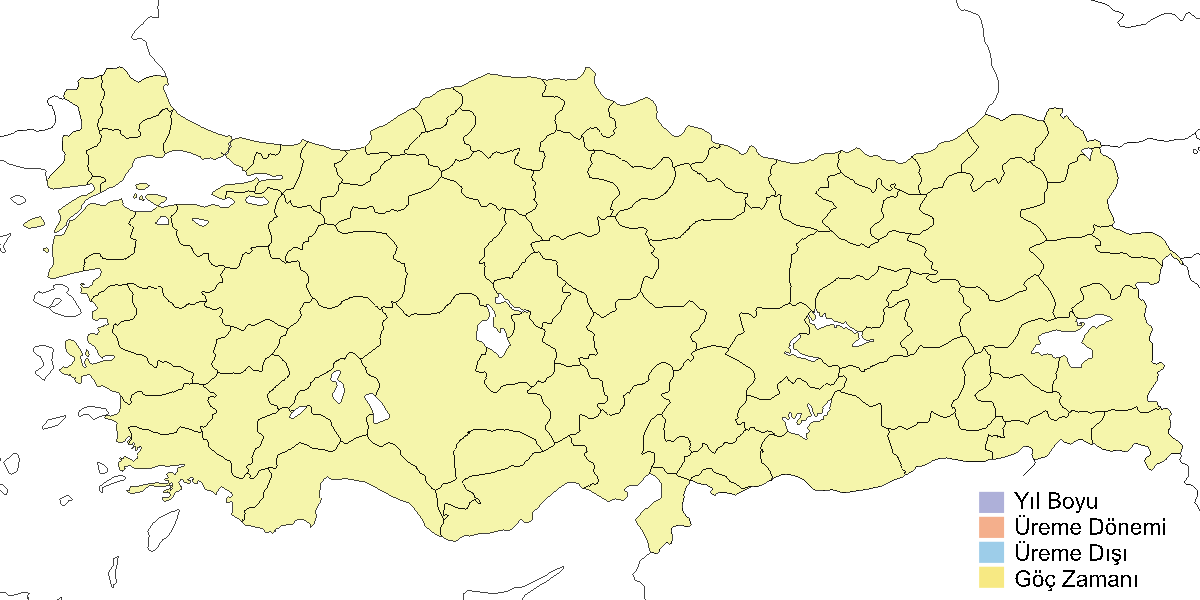
\includegraphics[keepaspectratio]{images/harita_Falco vespertinus.png}}

\textbf{Üreme}

\textbf{Yuvalama alanı:} Bulunan tek güncel üreme kaydı (Sinav \& Kıraç,
2023) Eskişehir Sivrihisar'da Seydi Deresi yakınındaki alan, bir
tarafında yoğun tarım yapılan, diğer tarafında ise mera bulunan bir
arazidir. Sulanan ve sulanmayan tarım uygulamaları yaygındır.\\
\textbf{Yuvası:} 24 Haziran 2016'da yapılan gözlemde, büyük ve izole bir
Ak Söğüt (\emph{Salix alba}) ağacındaki eski bir Saksağan (\emph{Pica
pica}) yuvasının kullanıldığı tespit edilmiştir. Başka yerlerde diğer
kuşların eski yuvalarında özellikle ekin kargası ve saksağan yuvalarında
yuvalar.\\
\textbf{Yumurta sayısı:} Bu konuda bilgi yoktur. Başka yerlerde
genellike 3-5 yumurta koyar.\\
\textbf{Üreme dönemi:} Başka yerlerde mayıs sonu-nisan başında yumurta
koyar. \textbf{İÇA:} Gözlem alanı 24 Haziran 2016'da ziyaret edilmiş ve
erişkin kuşlar yuvada aktif olarak gözlenmiştir. Ancak, 23 Temmuz
2016'daki ikinci ziyarette yuva ağacın altına düşmüş halde bulunmuş,
alanda erişkin birey, yumurta veya ölü yavruya rastlanmamıştır. Bu
durum, türün Türkiye'deki ilk belgelenmiş üreme girişimi olarak
kaydedilmiş olsa da, girişim başarısızlıkla sonuçlanmıştır. 8-14 Mayıs
1876'da Kayseri'de biri sürü görülmüştür (Danford, 1877-78)ve biraz daha
kuzeyde bir köyde üreme kaydedilmiştir. Bu durumun çok şüpheli olması
sadece lokalitenin konumuyla ilgili değil, aynı zamanda türün genelde
yaklaşık 2 hafta sonra üremeye başlamasından kaynaklanmaktadır.

\textbf{Alttürler ve Sınıflandırma}

Monotipik bir türdür.

\section{Ada Doğanı}\label{ada-doux11fanux131}

\emph{Falco eleonorae}, Eleonora's Falcon

\textbf{\emph{Lokal olarak nispeten az sayıda görülen yaz konuğudur.}}

Ege ve Akdeniz kıyılarında çok nadiren yuvalar. 15 Mayıs 2004'te İzmir
Karaburun'da 8 çift kaydedilmiştir. Başta Ege olmak üzere, farklı
bölgelerde düzenli aralıklarla yapılan kayıtlar, türün üreme durumunun
araştırılması açısından değer taşımaktadır (Eken, 1997c). Türün başka
bölgelerdeki yuvalama dönemi temmuz-eylül arasındadır. 1978'de Marmara
Adası'nda 18--21 çiftten oluşan bir koloni tespit edilmiştir (Kaymas,
1980). Çanakkale'de 17 Temmuz 2000'de 8 çiftin ``muhtemel üreme''
durumunda olduğu not edilmiştir (Kirwan \emph{vd.}, 2003). Ayrıca, son
yıllarda güneybatı kıyıları açıklarında da ürediği doğrulanmıştır.
Bununla birlikte, Marmara Adaları'nda Ekim 1994'te yapılan üç günlük
araştırmada türe rastlanamamıştır. 1971 yılı ekim başlarında Mersin
Gelindere yakınlarında muhtemelen Aydıncık Adaları'nda üreyebilir
(Warncke, 1972).

Ege ve Akdeniz kıyıları boyunca, genellikle 10 bireyi geçmeyen küçük
gruplar hâlinde, tahminen üreme dönemi öncesindeki yaz ziyaretleri
sırasında ve göç dönemlerinde düzenli olarak gözlenmektedir. İstisnai
yüksek sayılar arasında, 25 Haziran 1994'te Muğla'da 22 birey, 1990
Mayıs sonunda Uluabat Gölü ile Yeniköy arasında 29 birey, 1973 Haziran
sonunda Manyas Gölü'nde 30 birey ve 1988 başlarında Bodrum'da kaydedilen
112 birey yer almaktadır (Ristow \& Wink, 1995).

Tür üreme öncesi dağılma döneminde üreme alanlarından uzakta kaydedilir.
Genellikle kıyı sulakalanları, akarsu kenarları ve kayalık alanlarda
görülür; iç kesimlerde ise daha seyrektir. İç Anadolu'da yaz aylarında
nadiren rastlansa da, bazı bireyler eylül sonuna kadar kalabilir.
Ovalarda ve 1000 metreye kadar olan dağ eteklerinde yaygındır; nadir de
olsa 2000 metrenin üzerindeki alanlarda da gözlenmiştir. İstanbul
Boğazı'nda ilkbahar ve yaz başlarında seyrek olarak görülse de, ağustos
sonundan ekim başına kadar düzenli kaydedilir. Bu bireylerin
Marmara'daki üreyen popülasyonlara ait olduğu sanılmaktadır. Karadeniz
Bölgesi'nde dört kayıt mevcuttur; bunların en doğudaki Rize'dendir.
Benzer şekilde, Sivrikaya ve Doğu Anadolu'dan da birkaç gözlem
kaydedilmiştir. Doğu Anadolu'daki üç yeni kayıttan biri, 2 Ekim 1980'de
Kars Tuzluca'da dört bireylik bir grubun gözlenmesidir. Güneydoğu
Anadolu'dan ise Birecik, Cizre, Diyarbakır ve Gaziantep'ten toplam on
kayıt bildirilmiştir.

\pandocbounded{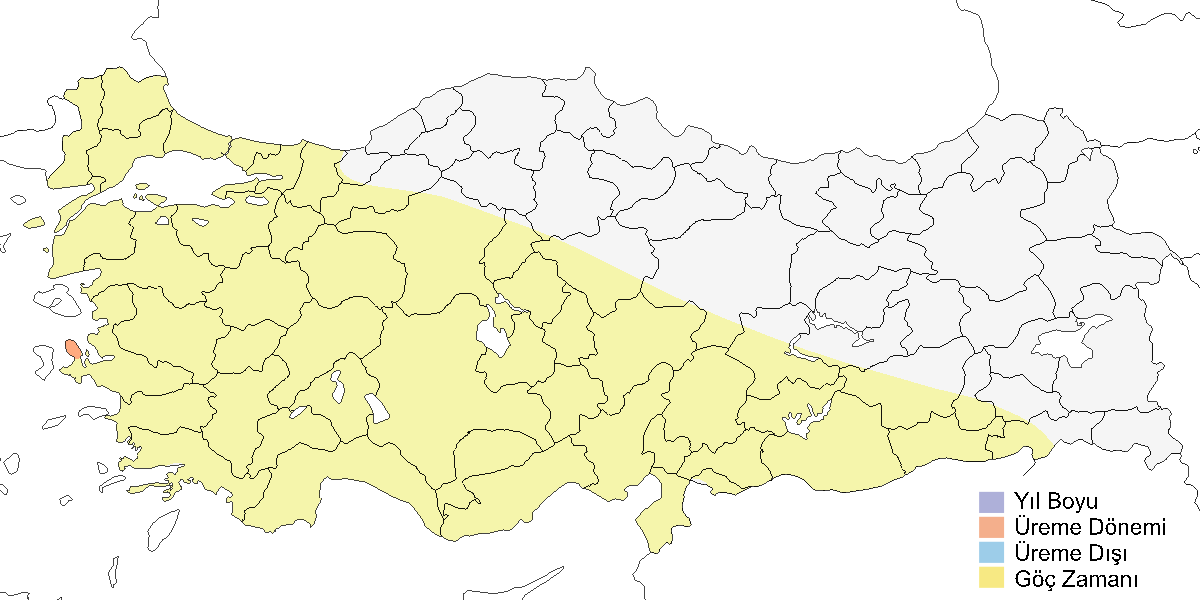
\includegraphics[keepaspectratio]{images/harita_Falco eleonorae.png}}

\textbf{Üreme}

\textbf{Yuvalama alanı:} Türkiye'den veri bulunmamaktadır. Diğer
bölgelerde çıplak kayalıklarda, yarıklarda ve yarlarda, özellikle
adalarda yuvalar.\\
\textbf{Yuvası:} Kayalık alanlara yapılan yuva basit bir oyuktur, içi
astarlanmaz.\\
\textbf{Yumurta sayısı:} Genellikle 2-3 yumurta bırakır.\\
\textbf{Üreme dönemi:} Yumurtlama temmuz sonunda gerçekleşir. Yavrular
ağustos sonunda çıkar ve eylül sonu ile ekim başında yuvayı terk eder.
Bu geç dönemdeki üreme, avladığı kuşların sonbahar göçüne denk geldiği
için yavrulara bol besin sağlar.

\textbf{Alttürler ve Sınıflandırma}

Monotipik bir türdür.

\section{Gri Doğan}\label{gri-doux11fan}

\emph{Falco concolor}, Sooty Falcon

\textbf{\emph{Rastlantısal konuktur.}}

24 Mayıs 1973'te Birecik'te biri açık, diğeri koyu donlu iki birey
gözlenmiş ve bu bireyler ayrıntılı şekilde tanımlanmıştır (Mertens,
1974). Aynı lokaliteden iki daha yeni kayıt bulunmaktadır: biri 15
Haziran 1999, diğeri ise 6 Temmuz 2001 tarihlidir (Kirwan \emph{vd.},
2003). Buna ek olarak, 4 Temmuz 1976 akşamı Birecik yakınlarında yarasa
avlarken gözlenen ve koyu donlu bir Ada Doğanı olarak tanımlanan bireyin
Gri Doğan olma olasılığı da bulunmaktadır {[}Beaman (1986);
@kasparek1986{]}. 1 birey ``Milleyha ve sahil şeridi'' alanında (Hatay)
23 Temmuz 2021 tarihinde \emph{E. Yoğurtçuoğlu} tarafından
kaydedilmiştir.

\pandocbounded{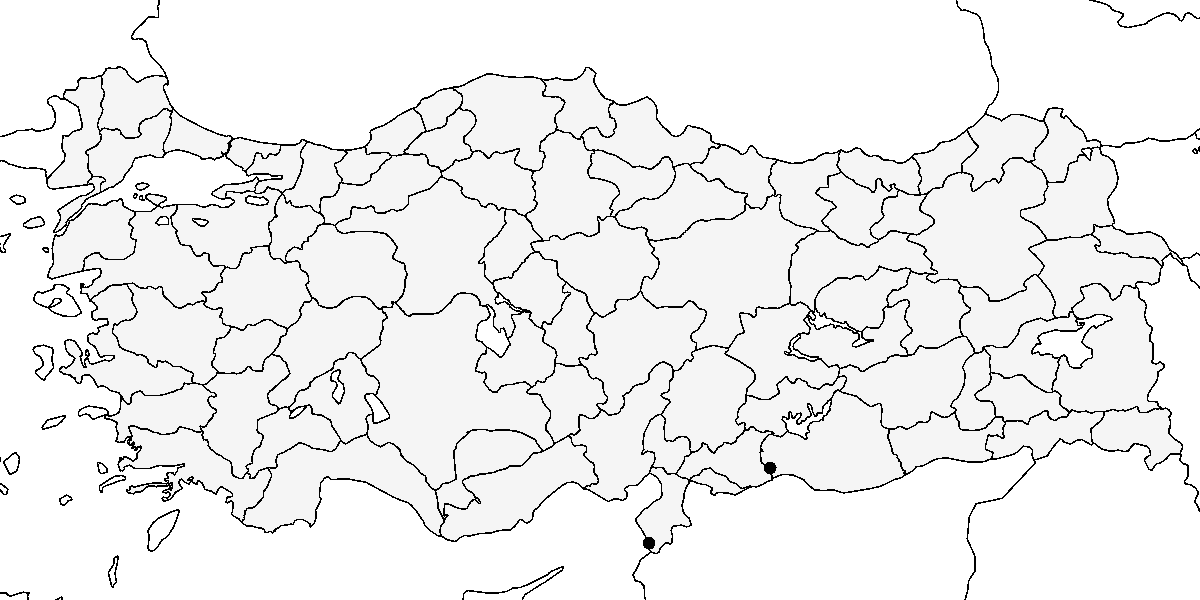
\includegraphics[keepaspectratio]{images/harita_Falco concolor.png}}

\textbf{Üreme}

Türkiye'de yuvalamaz. Yuvalama bölgesi Kızıldeniz çevresi, Hürmüz Boğazı
çevresi ve Kuzeydoğu Afrika çölleridir.

\textbf{Alttürler ve Sınıflandırma}

Monotipik bir türdür.

\section{Boz Doğan}\label{boz-doux11fan}

\emph{Falco columbarius}, Merlin

\textbf{\emph{Yaygın olarak nispeten çok sayıda görülen kış konuğudur.}}

Türkiye'nin tamamında yaygın olarak bulunur. Özellikle Orta ve Batı
Anadolu'da kışlayan bireylerin sayısı daha fazladır. Genellikle eylül
ortasından nisan ortasına kadar kaydedilir. Bununla birlikte, Trakya'da
mayıs başına kadar kalabilen bireyler olduğu gibi, istisnai olarak 20
Temmuz gibi erken bir tarihte Boğaziçi'nde gözlenmiş bir kayıt da
mevcuttur. Uygun sulakalanlarda, özellikle Karadeniz ve İç Anadolu'da
görülür. Toroslar'ın güneyinde ise görece nadirdir.

Başlıca yırtıcı göçü izleme noktalarında ekim sonlarında nadiren
kaydedilir. Bununla birlikte 1977 yılı ekim ortası ile sonu arasında
Borçka'da 21 birey kaydedilmiştir (Beaman, 1977). 2002 sonbaharında
Batum'da gözlenen toplam 972 birey ise türün Doğu Karadeniz üzerinden
gerçekleştirdiği göçün düşündüğümüzden çok daha yaygın olduğunu
göstermektedir (Balmer \& Kirwan, 2003).

\pandocbounded{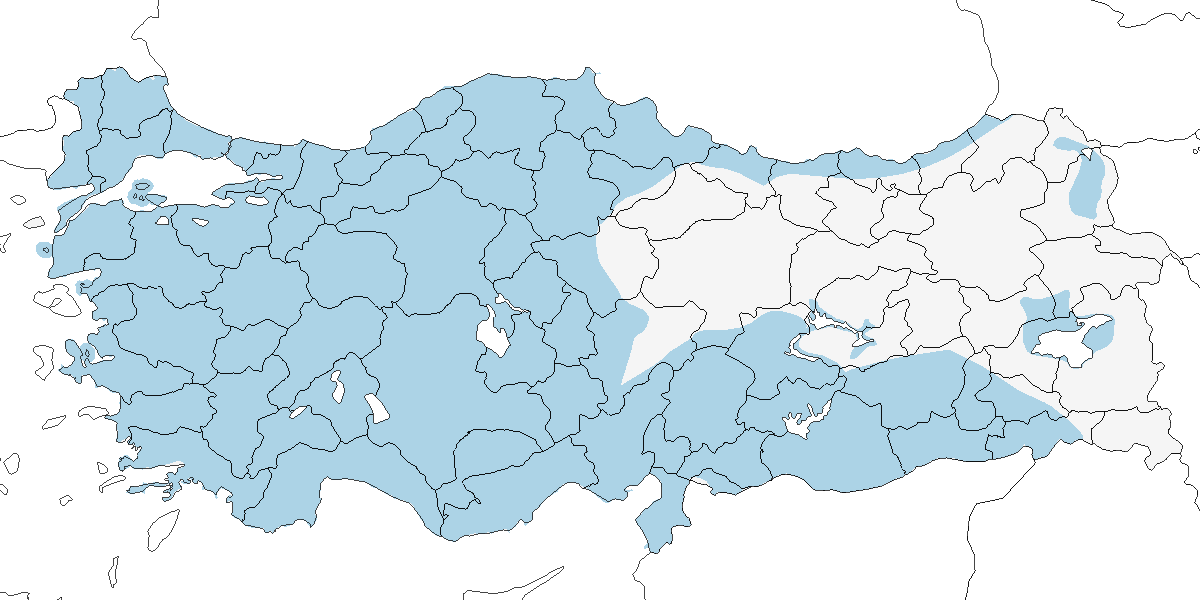
\includegraphics[keepaspectratio]{images/harita_Falco columbarius.png}}

\textbf{Üreme}

Türkiye'de yuvalamaz. Avrasya ve Kuzey Amerika'nın kuzey bölgelerinde
yuvalar.

\textbf{Alttürler ve Sınıflandırma}

En yaygın görülen alttürün, Avrupa ve Kuzeybatı Sibirya'da üreyen ve kış
aylarını Kuzey Afrika'ya kadar uzanan bölgelerde geçiren \emph{aesalon}
olduğu düşünülmektedir. Ancak Tring Doğa Tarihi Müzesi'ndeki Hume
Koleksiyonu'nda, İzmir'den geldiği belirtilen bir dişi örnek
(85.8.19.2483), Orta Kuzey Sibirya'da yuvalayan ve Kuzeydoğu Afrika ile
Orta Doğu'da kışlayan \emph{insignis} alttürüne ait olabilir (Bird,
1937) (; G. M. Kirwan kişisel gözlem). Öte yandan, Orta Asya
bozkırlarında yuvalayan \emph{pallidus} alttürü, Trabzon'dan toplanmış
bir örnekle belgelenmiştir (Vaurie, 1965) ve bu form Malatya
yakınlarında kışlayan bireylerden biri olabilir.

\section{Delice Doğan}\label{delice-doux11fan}

\emph{Falco subbuteo}, Eurasian Hobby

\textbf{\emph{Oldukça yaygın olarak ve çok sayıda bulunan yaz konuğu ve
geçit türüdür.}}

Genellikle az ağaçlı ovalar, bozkırlar ve dağlık bölgelerdeki açık
alanlarda 2800 metreye kadar olan yüksekliklerde kaydedilir; yalnızca
iki kayıtta 4000 metreye ulaşmıştır. Ayrıca korular, küçük ağaçlandırma
sahalarındaki açıklıklar, orman içi açıklıklar, ibreli ve yaprak döken
ormanlar; ovalar, tepelik ve dağlık bölgeler, nehir kenarındaki
plantasyonlar, tarım alanları ve kavaklıklarda da ürer. Ankara'da
bahçelerde düzenli olarak ürediği bilinmektedir; buradan 1945 yılına ait
iki çiftin üreme kaydı mevcuttur (Wadley, 1951).

Çoğunlukla nisan ortasından ekim başına kadar görülür, ancak mart
ortasından ekim sonuna kadar da kaydedilmiştir. Zonguldak Çatalağzı'ndan
bildirilen 1940'lı yıllara ait bir aralık kaydı vardır (Ogilvie, 1954),
ancak bu gözlemin hatalı olması muhtemeldir.

İlkbahar göçü mart ortasında başlar ve genellikle mayıs ortasında sona
erer; mayıs sonuna kadar az sayıda birey hâlâ geçiş yapabilir. Ana göç
izleme noktalarında genellikle düşük sayılarda kaydedilmiştir. 1976
sonbaharında Borçka'da 189 birey sayılmış (Andrews \emph{vd.}, 1977),
2002 sonbaharında ise Batum'da toplam 910 birey kaydedilmiştir.

\pandocbounded{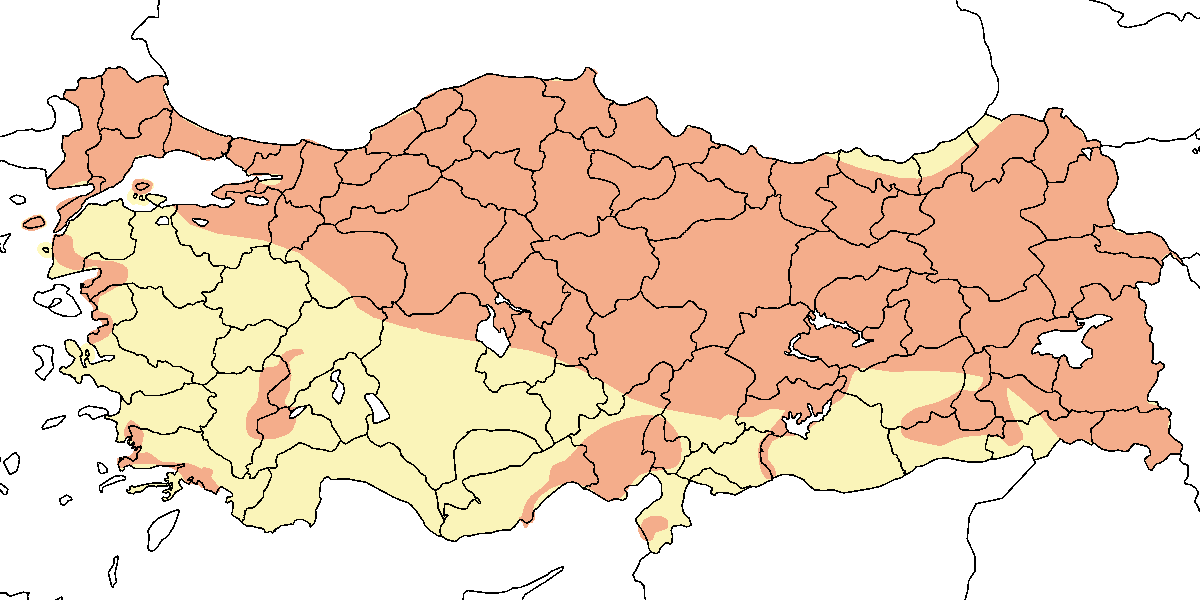
\includegraphics[keepaspectratio]{images/harita_Falco subbuteo.png}}

\textbf{Üreme}

\textbf{Yuvalama Alanı:} Ağaç üzerindeki eski kuş yuvalarıdır.
Ağaçlarda, özellikle diğer kuşların eski yuvalarını kullanarak ürer.
Türkiye'de yalnızca leş kargası yuvalarını kullandığı kaydedilmiştir.
Ancak ekin kargası ve saksağan yuvalarını da kullandığı tahmin
edilmektedir. Muhtemelen balıkçıl ve kara çaylak gibi türlerin ağaç
üzerindeki yuvalarını da kullanır. Yuvaya herhangi bir materyal
eklemez.\\
\textbf{Yuvası:} Diğer türlere ait eski yuvaları kullanır ve içine yuva
materyali eklemez.\\
\textbf{Yumurta sayısı:} Türkiye'den veri yoktur. Diğer bölgelerde
genellikle 3, nadiren 2 yumurtayla kuluçkaya yattığı bilinmektedir.\\
\textbf{Üreme dönemi:} Yumurtlama haziran ortasında başlar, yavrular
temmuz ortasında çıkar. Yavrular genellikle ağustos ortasında yuvadan
ayrılır. Gözlemler çiftleşmeden birkaç hafta önce yuvayı sahiplendiğini
ve bu dönemde oldukça gürültülü ve dikkat çekici olduğunu
göstermektedir. Kuluçka döneminde ise oldukça sessizdir. Mayıs ayındaki
yuvaların genellikle boş olması bu davranış modelini desteklemektedir.
\textbf{MAR:} 6 Mayıs 1997'de Beykoz'da bir çift yuvada gözlenmiş, 24
Haziran 1973'te Keşan'da yuvaya yiyecek taşıma davranışı kaydedilmiştir.
14 Ağustos 1966'da Çamlıca'da çam, meşe ve çalılıklar arasındaki bir
iğne yapraklı ağaçta yer alan yuvada dört yavru bulunmuş, bu yavrulardan
biri 2 Eylül'de, diğer üçü ise 4 Eylül'de yuvadan ayrılmıştır. Bu durum,
yumurtlamanın haziran sonu veya temmuz başında başladığını
göstermektedir. \textbf{EGE:} 20 Ağustos 1996'da Kuşadası'nda bir genç
birey görülmüştür. \textbf{AKD:} 10 Mayıs 1987'de Çukurova'da kur
davranışı sergileyen bir çift gözlenmiştir (Have \emph{vd.}, 1988). 8
Mayıs 1992'de Demirkazık yakınlarında bir yuva tespit edilmiştir.
\textbf{KAR:} Kızılırmak Deltası'nda 7 Temmuz--6 Ağustos 1971 tarihleri
arasında 12 aktif yuva kaydedilmiştir. Bu yuvalardan birinde 27 Temmuz
1971'de yumurta görülmüş, 29 Ağustos 1984'te ise bir erişkinin genç
bireye yiyecek taşıdığı gözlenmiştir (Dijksen \& Kasparek, 1985).
1992'de bölgedeki popülasyonun 23 çifti Yörükler Ormanı'nda olmak üzere
toplamda 45--50 çift olduğu tahmin edilmiştir. En az beş aktif yuvanın
ağaç üzerinde olduğu belirtilmiştir. Bu yuvalardan biri 17 Mayıs 1992'de
bulunmuş, ancak 10 Haziran'da yuvadan ses gelmemiştir (Hustings \& Dijk,
1994). Bu durum, kuluçkanın henüz başlamadığını göstermektedir. Aynı
bölgedeki İspir'de 11 Mayıs 1986'da yuvada erişkinler görülmüş, 15
Haziran 1987'de üreme teyit edilmiştir. Gelinkaya'da 1992 Eylül
başlarında erişkinlerin yuvaya yiyecek taşıdığı gözlenmiştir (Gosney,
1993). \textbf{DOA:} 30 Mayıs 1969'da Edremit'te kur davranışı
sergileyen bir çift gözlenmiş, 26 Haziran--2 Temmuz 1987'de aynı bölgede
yuva yapım süreci gözlenmiştir. Haziran 1987 başlarında Çatak'ta üreme
kesin olarak kaydedilmiştir. 19 Mayıs 1935'te Malatya yakınlarında bir
yuva bulunmuştur (Bird, 1937). 18 Haziran 2004'te Güzelsu yakınlarında
yaklaşık 12 m yüksekliğindeki kavaklıktaki bir ekin kargası yuvasından
havalanan bir birey kaydedilmiş, aynı alanda başka bir çiftin sesi
duyulmuştur. Yuva kontrol edilmemiştir ancak kuluçkanın başlamadığı
tahmin edilmektedir. Bu durum erken yumurtlama ya da tamamlanmamış
kuluçkaya işaret edebilir.

\textbf{Alttürler ve Sınıflandırma}

Türkiye'de nominat alttürü bulunur.

\section{Bıyıklı Doğan}\label{bux131yux131klux131-doux11fan}

\emph{Falco biarmicus}, Lanner Falcon

\textbf{\emph{Lokal olarak az sayıda bulunan yerlidir.}}

Türkiye'de üreyen bir tür olarak ilk kez 1933'te Ilgaz Dağları'ndan
kaydedilmiş ve bu kayıt (Kumerloeve \& Niethammer, 1935) tarafından
teyit edilmiştir. Ancak türün üreme durumu ve yayılışı hâlâ tam olarak
açıklığa kavuşmamıştır. Geçmişte büyük ve orta boy doğanlarla, özellikle
uludoğan, gökdoğan ve açık donlu ada doğanı ile sıkça karıştırıldığı
için, bildirilen kayıtların önemli bir kısmının hatalı olabileceği
düşünülmektedir. Trakya'da bulunmadığı, Trakya dışındaki bölgelerde ise
nadir yerli bir tür olduğu kabul edilmektedir. Karadeniz'de çok lokal
bir yayılışa sahiptir. Genellikle kıraç bozkırlarda ve ağaçsız dağlık
alanlarda görülür, nadiren 3000 metreye kadar ulaşan ağaçlı bölgelerde
de kaydedilmiştir.

Tüm ülkede göç döneminde ve kış aylarında üremeye kıyasla daha yaygın
olmakla birlikte, genel olarak nadir bir türdür. Ana göç izleme
alanlarında eylül ortasından ekim ortasına kadar gözlenmiştir. Kışın
daha çok kıyı alanlarında ve sulakalan çevrelerinde görülür.

Doğancılar için yumurta ve yavruların toplanmasından dolayı, popülasyonu
çok düşük seviyededir. Bıyıklı ve Ulu Doğan, doğancıların özel ilgisini
çeker ve üreyen erişkinler, yavruları ile yumurtaları kaçakçılar
tarafından hedef alınır. Muhbir köylüler, profesyonel yakalayıcılar ve
kaçakçılar, yerleşen bireyler üzerinde ciddi bir baskı oluşturur. Bu
baskı sonucunda, yerleşen ve üreyen çiftler birkaç yıl içinde tespit
edilmekte ve yasadışı yollarla yakalanarak yurt dışına kaçırılmaktadır.
Bu nedenle, yeni yerleşen bireyler çoğunlukla kısa sürede ortadan
kaybolmaktadır.

\pandocbounded{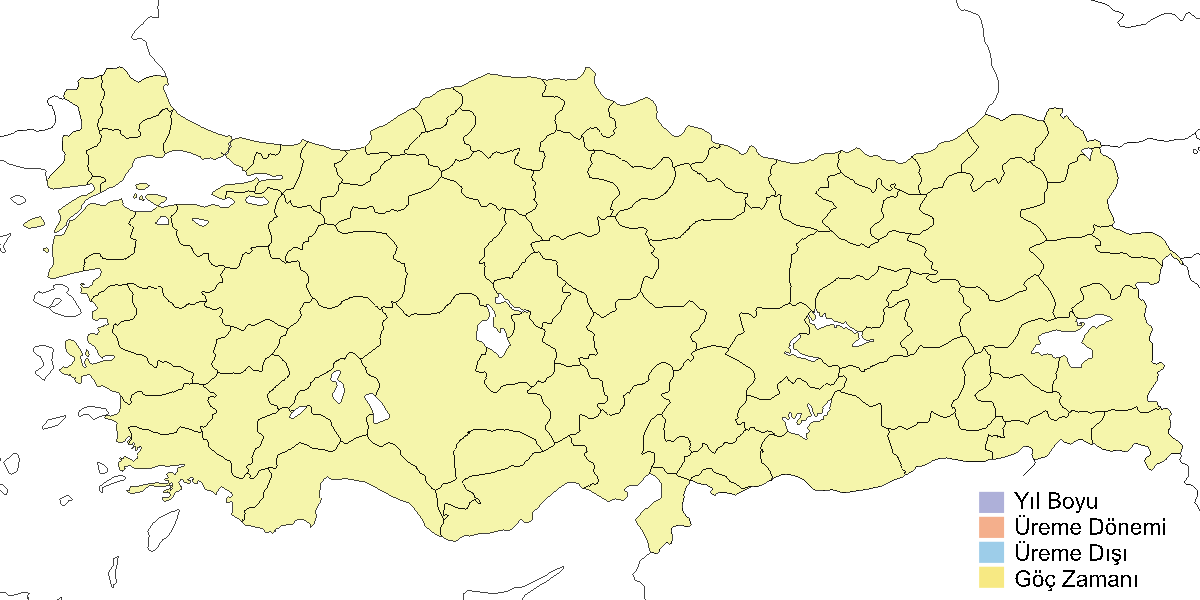
\includegraphics[keepaspectratio]{images/harita_Ficedula albicollis.png}}

\textbf{Üreme}

\textbf{Yuvalama Alanı:} Yarların ve kayalık katmanların olduğu açık
alanlarda ürer. İç Anadolu'da, Sarıyar Barajı'ndaki kayalıklarda ve
Beypazarı'nın kuzeyindeki 100 m yükseklikte ve 1 km uzunluğundaki
vadinin kayalıklarında birer çift üremiştir (Magnin \& Yarar, 1997).
\textbf{Yuvası:} Türkiye'den veri yoktur. Diğer bölgelerde yuvası
yalnızca hafif kazılmış bir çukurdur ve yuva materyali içermez.\\
\textbf{Yumurta sayısı:} Diğer bölgelerde genellikle 3-4 yumurta ile
kuluçkaya yatar.\\
\textbf{Üreme dönemi:} Nisan ayrında yumurta koyar. Yavrular mayıs ayı
başında çıkar. \textbf{İÇA:} 8 Mayıs 1961'de Karapınar yakınlarındaki
kayalıklarda içinde üç 10 günlük yavru ve henüz çatlamamış bir yumurta
bulunan bir yuva kaydedilmiştir (Warncke, 1964-\/-65). Bu kayıt,
yumurtlamanın 3 Nisan civarında başladığını göstermektedir. Aynı
bölgede, 8 Nisan 1984'te Kızılcahamam'daki kayalıklarda iki erişkin
birey, 12 Mayıs 1984'te ise bir çift gözlenmiştir (Barış \emph{vd.},
1984).

\textbf{Alttürler ve Sınıflandırma}

Türkiye'de \emph{feldeggi} alttürü bulunur.

\section{Ulu Doğan}\label{ulu-doux11fan}

\emph{Falco cherrug}, Saker Falcon

\textbf{\emph{Nispeten yaygın ancak az sayıda bulunan yerlidir. Kışın
göç alır.}}

Üreme döneminde genellikle yüksek rakımlı, kıraç ovalarda ve bu alanlara
yakın dağlık bölgelerde bulunur. Önceleri, muhtemelen 1966'ya kadar Ege
ve Marmara'da yuvalamıştır. 1875'te İstanbul çevresinde yuva yaptığı,
1950'lerin ortalarına kadar da şehir yakınlarında düzenli olarak
gözlendiği bilinmektedir (Kumerloeve, 1961).

Göç döneminde, özellikle sonbahar ve kış aylarında tüm ülkede biraz daha
yaygın olarak gözlenir. Üç ana göç izleme noktasında, ağustos ortasından
ekim ortasına kadar kaydedilmiştir.

Bıyıklı ve ulu doğan, doğancıların özel ilgisini çeken türlerdendir. Bu
nedenle, üreyen erişkinler, yavrular ve yumurtalar kaçakçılar tarafından
hedef alınır. Muhbir köylüler, profesyonel yakalayıcılar ve kaçakçılar
yerleşen bireyler üzerinde ciddi bir baskı oluşturur. Bu baskı
sonucunda, yerleşen ve üreyen çiftler birkaç yıl içinde tespit
edilmekte, yasadışı yollarla yakalanarak yurtdışına kaçırılmaktadır.
Dolayısıyla, yeni yerleşen bireyler genellikle kısa sürede
kaybolmaktadır.

\pandocbounded{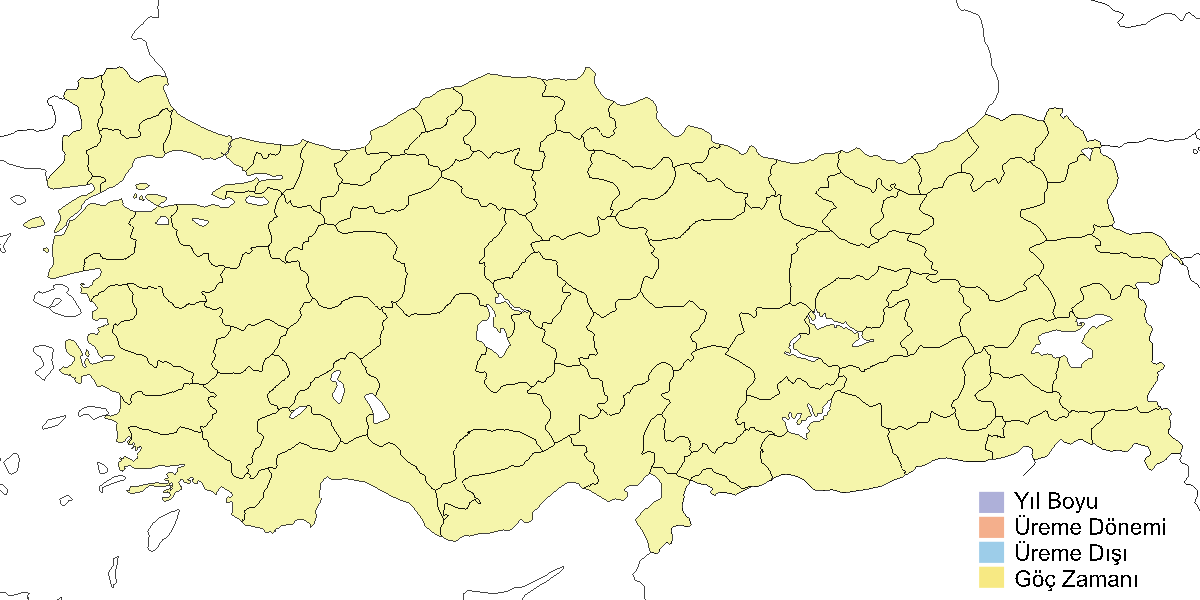
\includegraphics[keepaspectratio]{images/harita_Ficedula albicollis.png}}

\textbf{Üreme}

\textbf{Yuvalama Alanı:} Sıklıkla Orta Anadolu'daki kuru, açık bozkırlar
ve geniş vadilerin yakınındaki kaya yarlarında, doğudaki yüksek
vadilerdeki koyak ve yarlarda yuvalar. Yuvasını yüksek kayalıklardaki
girinti ve çıkıntılara yapar. Tuz Gölü'nde eski ve uzak bir adada
zeminden 3 metre yüksekte bir yuva da kaydedilmiştir. Aynı zamanda eski
kızıl şahin yuvalarına da yuva yapar. Macaristan'da ağaç üzerine yuva
yaptığı bilinmekle birlikte, Türkiye'den bu konuda bir kayıt yoktur.\\
\textbf{Yuvası:} Yalnızca hafifçe kazılmış bir çukurluktur ve içinde
yuva materyali bulunmaz. Bazı yuva yerleri ardışık yıllarda tekrar
kullanılır.\\
\textbf{Yumurta sayısı:} Türkiye'de birery yuvada 3 ve 4 yumurta
kaydedilmiştir. 4 yuvada 1 yavru, 2 yuvada 2 yavru, 2 yuvada 3 yavru, 1
yuvada 4 yavru ve 1 yuvada 5 yavru kaydedilmiştir.\\
\textbf{Üreme dönemi:} Mart ortasında ürer. Nisan ayından itibaren
yumurta koyar, yavrular mayıs ayından itibaren görülür. \textbf{KAR:} 26
Haziran 1978'de Merzifon'da bir yavru, 18 Ağustos 1989'da İspir'de 2
erişkin ve 1 yavru gözlenmiştir. Ayrıca, Tring Doğa Tarihi Müzesi'nde
bulunan ve 22 Nisan 1872'de Türkiye'den toplanmış olduğu belirtilen 4
yumurta kaydı vardır. \textbf{İÇA:} 1966'da Tuz Gölü'ndeki bir çiftin en
az 1, 1967'de ise 2 yavruyu aynı anda büyüttüğü, 1968 ve 1969 yıllarında
da erişkinlerin aynı bölgede bulunduğu kaydedilmiştir. Aynı adada
açılmamış yumurtalar ve 3 yavru görülmüştür. 31 Mayıs 1971'de yaklaşık
25 günlük olan bu yavrular, yumurtlamanın yaklaşık 7 Nisan'da
başladığını göstermektedir. 9 Mayıs 1975'te Şereflikoçhisar'ın
kuzeyindeki bir yuvada bulunan yavru, yumurtlamanın mart sonunda
olduğunu işaret etmektedir. 1 Haziran 1972'de Hasan Dağı'ndaki bir
oyukta gözlenen 3 haftalık yavru, yumurtlamanın 11 Nisan'da başladığını
göstermektedir. 7--30 Haziran 1977'de Ankara'nın doğusundaki iki yuvada
sırasıyla 2 ve 4 yavru bulunmuştur (Schubert, 1979). 26 Nisan 2007'de
Karadağ'da, hafif kazılmış geniş bir kaya çıkıntısı üzerindeki yuvada 10
günlük 5 yavru; 6 Mayıs 2007'de Yeşilhisar yakınlarında 3 haftalık 3
yavru bulunan bir yuva kaydedilmiştir. 25--26 Nisan 1980'de Konya
yakınlarında erişkin bireylerin yuvaya birkaç kez indiği gözlenmiştir.
27 Nisan 1968'de Karapınar'ın doğusunda bir çift kaydedilmiştir. 22
Temmuz 1971'de Ürgüp yakınlarında 2 yavrulu bir erişkin, 21 Haziran
1990'da Selima'da gözlenmiştir. \textbf{DOA:} 10 Mayıs 1970'te Tutak ile
Namur arasında bir yuva kaydedilmiştir. 1 Haziran 1971'de Erciş'te
muhtemel bir yuvanın yakınında kızıl şahini kovalayan iki erişkin
gözlenmiştir. 9 Haziran 1975'te Ahtamar Adası'nda yuvaya yiyecek taşıyan
erişkinler, 6 Haziran 2002'de Doğubayazıt ile Karabulak arasında bir
yuvada 2 yavru kaydedilmiştir. \textbf{GDA:} 8 Nisan 1971'de Fırat
Nehri'nin Suriye sınırına yakın kesimlerinde 3 yumurtalı bir yuva
gözlenmiş, yuvada kuluçkaya yatan dişinin av yakalayan erkeğe yemeği
bıraktığı kaydedilmiştir. Aynı yuvanın altında 4 çift söğüt serçesi
üremiştir (Warncke, 1972).

\textbf{Alttürler ve Sınıflandırma}

Nominat alttür bulunmaktadır.

\section{Gökdoğan}\label{guxf6kdoux11fan}

\emph{Falco peregrinus}, Peregrine Falcon

\textbf{\emph{Yaygın olarak çok sayıda bulunan yerli ve göçmendir.}}

Yaygın, lokal olarak yerli ve kısmen göçmen bir türdür. Ege, Karadeniz
ve Akdeniz bölgelerinde daha sık görülür. Genellikle 800 metrenin
üzerindeki tepelik ve dağlık bölgelerde ürer ancak bazı bölgelerde deniz
kıyısındaki kayalıklarda da yuvalar.

Üreme dönemi dışında daha dağınık yayılır ve batı bölgelerindeki kıyısal
ovalarda sık sık gözlenir. Muhtemelen daha kuzeyden gelen bireyler kış
döneminde Türkiye'ye ulaşır. Ana göç izleme noktalarında az da olsa
kaydedilmiştir; bu gözlemler 22 Ağustos ile 21 Ekim tarihleri
arasındadır.

\pandocbounded{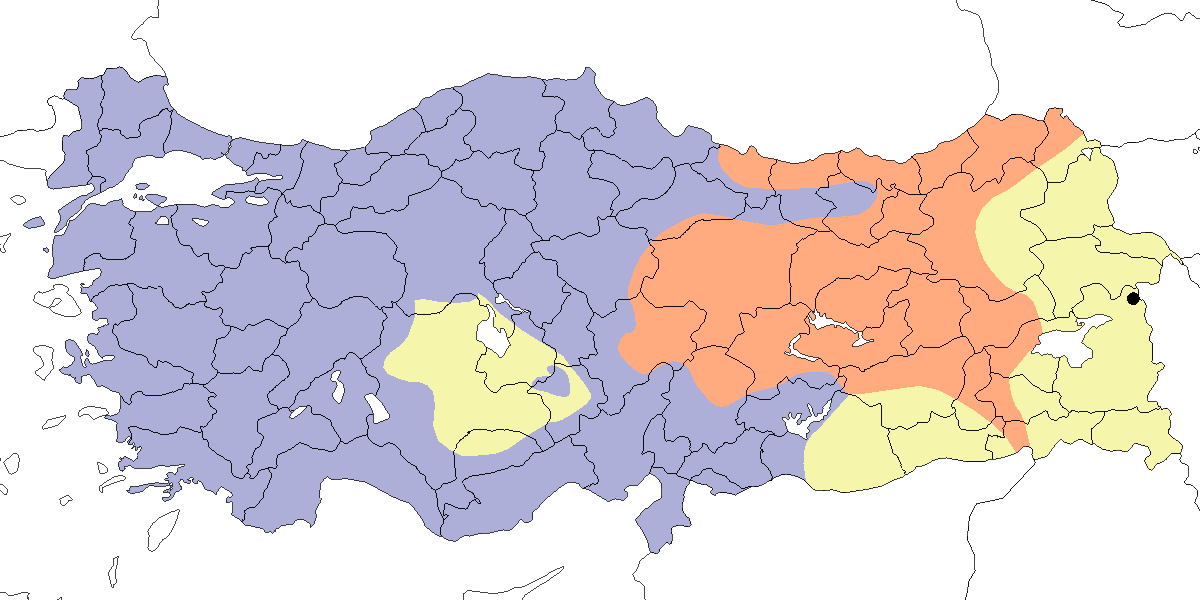
\includegraphics[keepaspectratio]{images/harita_Falco peregrinus.png}}

\textbf{Üreme}

\textbf{Yuvalama Alanı:} Tepelik ve dağlık alanlarda, deniz seviyesinden
2800 m'ye kadar olan yüksekliklerde yuvalar. Akdeniz kıyılarındaki
kayalık alanlardan Aladağlar'a kadar geniş bir yükseklik aralığında
üreyebilir. Yuvasını kayalıklardaki çıkıntılar, oyuklar ve vadilerde
yapar.\\
\textbf{Yuvası:} Yuva, herhangi bir malzeme kullanılmadan oluşturulan
sığ bir çukurluktur.\\
\textbf{Yumurta sayısı:} Türkiye'deki yuvalarda yumurta sayısına dair
veri bulunmamaktadır. Diğer ülkelerde genellikle 3-4 olmak üzere 2-6
yumurta bırakır. 1 yuvada 2, başka bir yuvada 3 yavru kaydedilmiştir.\\
\textbf{Üreme dönemi:} Türkiye'deki veriler sınırlı olsa da,
yumurtlamanın mart sonu-nisan, yavruların uçmasının ise mayıs
sonu-haziran arasında olduğu anlaşılmaktadır. Yumurtadan çıkan yavru
yaklaşık iki ay sonra yuvadan uçmakta, ebeveynlerinden ise iki ay sonra
tamamen ayrılmaktadır. \textbf{MAR:} 1970'te Uludağ'da 4 bireyden oluşan
olası bir aile grubu ağustos ortasından eylül sonuna kadar gözlenmiştir.
Bu durum, yumurtlamanın mart ortasında gerçekleştiğini düşündürmektedir.
\textbf{EGE:} 16 Mayıs 1987'de Adrasan kıyı kayalıklarında 2 çift yuva
yapmıştır. 13 Nisan 1971'de Gelindere'nin batısındaki kıyı
kayalıklarında bir yuvada yaklaşık 14 günlük 3 yavru gözlenmiştir, bu da
yumurtlamanın şubat sonunda başladığını göstermektedir. \textbf{AKD:} 23
Mart 1993'te Taşucu'nun kuzeyindeki kayalıklarda kur yapan bir çift, 15
Nisan 1993'te Aydıncık'ın doğusunda üreme alanını savunan bir çift
kaydedilmiştir. \textbf{KAR:} 21 Nisan 1993'te Çat'ta iki erişkinin bir
kaya kartalına saldırgan davranış gösterdiği kaydedilmiştir.
\textbf{İÇA:} 25 Mayıs 1992'de Hasan Dağı'nda, yüksek kayalıklarda
içinde 3-4 haftalık iki yavru olan bir yuva kaydedilmiştir. Bu tarih,
yumurtlamanın mart sonunda başladığını göstermektedir. 3 Haziran 1970'te
Ürgüp'te kayalık alanda daireler çizen bir dişi gözlenmiş, 22 Temmuz
1970'te aynı bölgede tüylenmiş bir yavru kaydedilmiştir. \textbf{DOA:}
25--30 Mayıs 1992 tarihleri arasında Van civarında 11 erişkin gözlenmiş,
bunlardan iki çifti uygun üreme habitatında kur davranışı sergilemiştir.
\textbf{GDA:} 3 Temmuz 1970'te Birecik'te bir yuva, 26 Mart 1973'te
Karkamış'ta içinde bir yumurta bulunan başka bir yuva kaydedilmiştir.
Ancak bu yumurtanın kuluçkaya ulaşmadığı düşünülmektedir. 15 Haziran
1996'da Işıklı'da yiyecek taşıyan bir erişkin gözlenmiştir.

\textbf{Alttürler ve Sınıflandırma}

Tüm ülkede üreyen yerli popülasyon \emph{brookei} alttürüne aittir. Uzun
mesafe göçmeni olan \emph{peregrinus} ve \emph{calidus} alttürleri göç
döneminde ve kışın Türkiye'de bulunur (Shirihai \& Spaar, 2000).
Ortadoğu'da görülen \emph{pelegrinoides} alttürüne ait Türkiye'deki tek
kesin kayıt, 12 Haziran 2012'de Van Çaldıran'da M. Zenginer ve S. Bekir
tarafından fotoğraflanan genç bireydir. Van Gölü ve doğusunda gökdoğan
nadir görüldüğünden, Kuzey İran'da üreyen kızıl enseli doğanların
(\emph{pelegrinoides}) bu bölgeyi sıklıkla ziyaret etmesi olasıdır. Bu
alttür ilk kez Ağustos 1990'da Birecik'te yapılan bir gözlemle gündeme
gelmiş (Gosney, 1996), Haziran 1994'te ise aynı alanda H. Shirihai ve
Francis tarafından kaydedilmiştir.

\section{İskender Papağanı}\label{iskender-papaux11fanux131}

\emph{Psittacula eupatria}, Alexandrine Parakeet

\textbf{\emph{Lokal ve çok sayıda bulunan yerlidir. Kafes kaçkınıdır.}}

Türkiye'de artık iyice yerleştiği düşünülen egzotik bir türdür. İlk kez
20 Şubat 1998'de Ankara'da, yeşil papağanlarla birlikte geceleyen küçük
bir grup içinde bir birey kaydedilmiştir (Boyla, Aydemir \& Eken, 1998).
Daha sonra, 2003 ve 2004 yıllarında İstanbul'da ürediği tespit
edilmiştir. Bunun dışında güneybatıda ve Güneydoğu Anadolu'da, Mayıs
2004'te Diyarbakır'da gözlenmiştir. Birçok gözlemcinin yeşil renkte bir
papağan gördüğünde bunu doğrudan yeşil papağan olarak tanımlaması
nedeniyle, bu türün sanıldığından daha yaygın olması mümkündür.

\pandocbounded{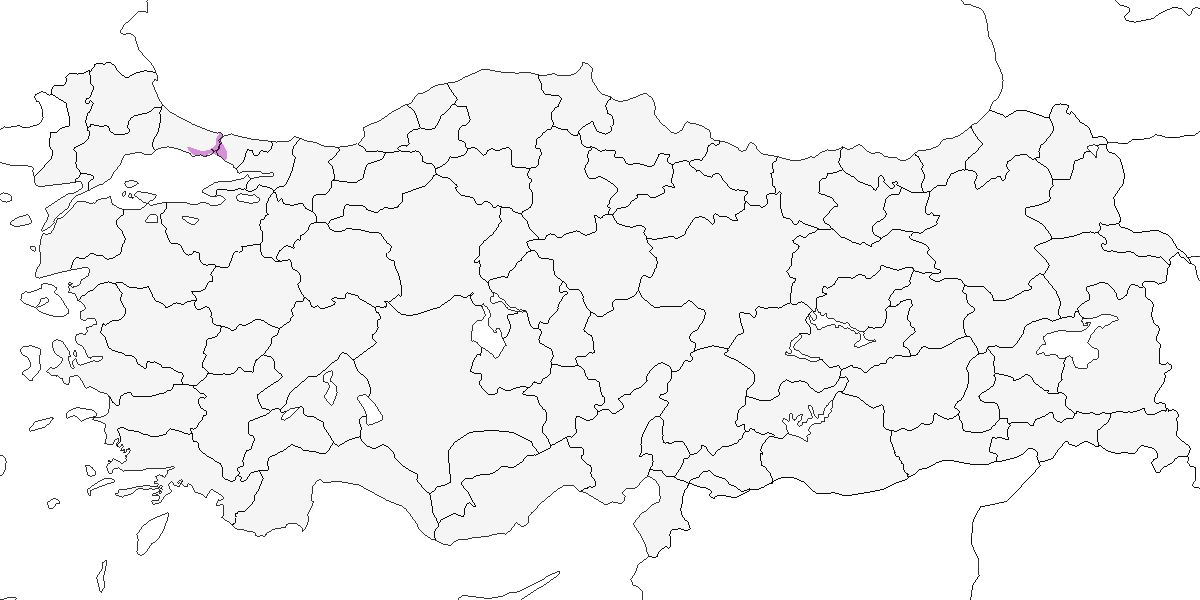
\includegraphics[keepaspectratio]{images/harita_Psittacula eupatria.png}}

\textbf{Üreme}

\textbf{Yuvalama Alanı:} Ağaç kovuklarında ya da benzeri korunaklı
alanlarda yuvalar.\\
\textbf{Yuvası:} Türkiye'deki gözlemler, ağaç kovuklarının
kullanıldığını göstermektedir.\\
\textbf{Yumurta sayısı:} Türkiye'de bilinmemektedir.\\
\textbf{Üreme dönemi:} İncelenmemiştir. \textbf{MAR:} 2003 yılında
İstanbul Topkapı Sarayı'nda türün ürediği, yuvası ve yavrusunun
fotoğraflandığı kaydedilmiştir. Aynı yıl, 15 Ekim'de İstanbul Gülhane
Parkı'nda bir çift gözlenmiş, dişinin bir ağaç kovuğuna girdiği ve
erkeğin saldırgan biçimde bir leş kargasına daldığı rapor edilmiştir.

\textbf{Alttürler ve Sınıflandırma}

Hangi alttürün olduğu bilinmemektedir.

\section{Yeşil Papağan}\label{yeux15fil-papaux11fan}

\emph{Psittacula krameri}, Rose-ringed Parakeet

\textbf{\emph{Lokal ve çok sayıda bulunan yerlidir. Kafes kaçkınıdır.}}

Ülkemizde ilk kez Haziran 1990'da Göksu Deltası'nda ve Eylül 1991'de
İstanbul'da kaydedilmiş (Kasparek, 1992), ancak daha sonra 1975 ve 1976
yıllarında Ankara'dan da erken kayıtların olduğu anlaşılmıştır (Kasparek
\& Bilgin, 1996). Ardından Boyla ve arkadaşları, bu kaçak türün
Türkiye'deki durumunu ortaya koyan kapsamlı bir değerlendirme yapmış ve
türün İstanbul'da en azından 1990 Mart'ından itibaren bulunduğunu,
İzmir'de ise muhtemelen 1950'lerden bu yana görüldüğünü belgelemiştir.
Bu süreci takiben, türün sayılarında hızlı bir artış yaşanmış ve yayılış
alanı belirgin biçimde genişlemiştir (Kirwan \emph{vd.}, 2003).
Günümüzde tür, batı ve orta bölgelerdeki tüm büyük şehirlerde
görülmektedir. İstanbul'da en fazla 450, İzmir'de 250 bireyden oluşan
sürüler kaydedilirken, Ankara'da en yüksek sayı 35 bireydir. Ayrıca,
kırsal bölgelerde de birkaç kaydı mevcuttur. Akdeniz ve Güneydoğu
Anadolu'da, doğuda Diyarbakır ve Cizre'ye kadar pek çok yerleşimde
görülmektedir.

\pandocbounded{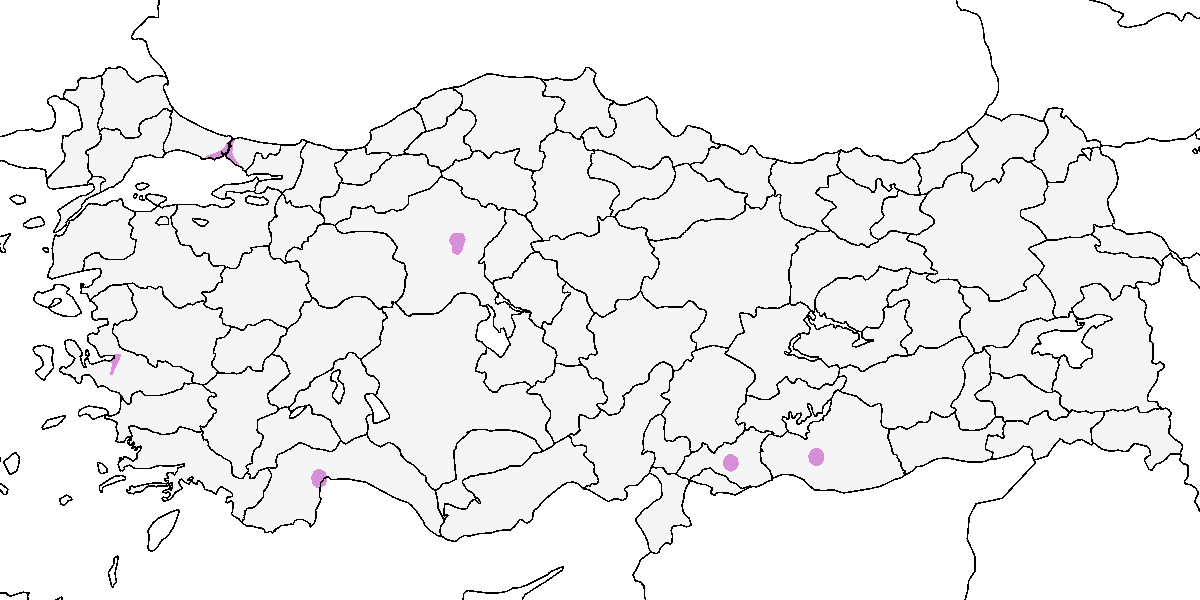
\includegraphics[keepaspectratio]{images/harita_Psittacula krameri.png}}

\textbf{Üreme}

\textbf{Yuvalama Alanı:} Diğer bölgelerde olduğu gibi Türkiye'de de
kovuklara yuva yapar. Yuva genellikle ağaç kovuklarında, bazen kaya
oyuklarında veya binalardaki deliklerde bulunur. Yuva astarlanmaz.\\
\textbf{Yuvası:} Kovuk içerisine astarsız olarak kurulur.\\
\textbf{Yumurta sayısı:} Türkiye'den kesin bilgi yoktur. Diğer
bölgelerde ortalama yumurta sayısı 4 olup, 3 ile 6 arasında
değişmektedir.\\
\textbf{Üreme dönemi: MAR:} Mayıs 1990'da İstanbul Bebek Arnavutköy'de
bir çiftin cami minaresinde yuvaladığı kaydedilmiştir. 31 Mayıs 2001'de
İstanbul Gülhane Parkı'nda kullanılan bir yuva bulunmuş ve başka birçok
çiftin varlığı koloniyi işaret etmiştir. \textbf{EGE:} 16 Mayıs 1995'te
İzmir Bornova'da, eski bir binadaki bir delikte yuvaladığı teyit
edilmiştir. \textbf{İÇA:} 1997'de Ankara Eymir Gölü'ndeki koruda bir
çiftin büyük ihtimalle ürediği düşünülmüştür (Boyla \emph{vd.}, 1998).

\textbf{Alttürler ve Sınıflandırma}

Alttürleri ayrıntılı olarak incelenmemiştir. Ortadoğu'daki çoğu
popülasyonun, esas olarak Hindistan Yarımadası'nda yaşayan borealis
alttürüne ait olduğu düşünülmektedir (Juniper \& Parr, 1998).

\part{Ötücüler}

\chapter{İspinozlar - Çinteler}\label{ispinozlar---uxe7inteler}

\section{İspinoz}\label{ispinoz}

\emph{Fringilla coelebs}, Common Chaffinch

\textbf{\emph{Yaygın olarak çok sayıda bulunan yerli ve kış
göçmenidir.}}

İç Anadolu, Güneydoğu Anadolu ve Doğu Anadolu'da nispeten lokal bir
türdür ve özellikle yerleşim çevresindeki tarım alanlarında yoğunlaşır.
Bu bölgelerde muhtemelen kısmen göçmen ya da irtifa göçmeni olarak
bulunur. Bitki örtüsünün geliştiği her türlü habitatta ürer. Ancak en
yaygın olduğu yerler Karadeniz Bölgesi ve Trakya'daki dağlık alanlardır;
burada 1100--2000 metreler arasındaki ibreli ve karışık ormanlarda
gözlenir.

Geçit dönemlerinde çok daha yaygındır. Özellikle ekim ayının ilk üç
haftasında, ülkenin kuzeyinde geniş bir cephe boyunca yüksek sayılarla
geçiş yapar. 24 Eylül ve 8 Kasım 1966 tarihlerinde İstanbul Boğazı'ndan
toplam 8865 birey, 18 Ekim 1980'de ise Küçük Çamlıca'dan 727 birey
geçmiştir. Göç hareketi ağustos başında başlar ve en azından kasımın ilk
haftasına kadar sürer; güney bölgelerde bu dönem daha da uzayabilir. En
erken kayıt 20 Ağustos, en geç kayıt 8 Kasım'dandır. İlkbahar göçü mart
ve nisan aylarında gerçekleşir; Erzurum'da 16 Mart--16 Nisan tarihleri
arasında önemli sayılarda birey gözlenmiştir.

Marmara, Ege, Akdeniz ve daha seyrek olarak Karadeniz bölgelerinde,
uygun habitatlarda ekim başından nisan ayına kadar büyük sayılarla
kışlar. Ancak bu mevsimde nadiren çok yüksek yoğunluklara ulaşır.
Örneğin, 1990--91 kışında Antalya'da yüzlerce birey kaydedilmiştir.

\pandocbounded{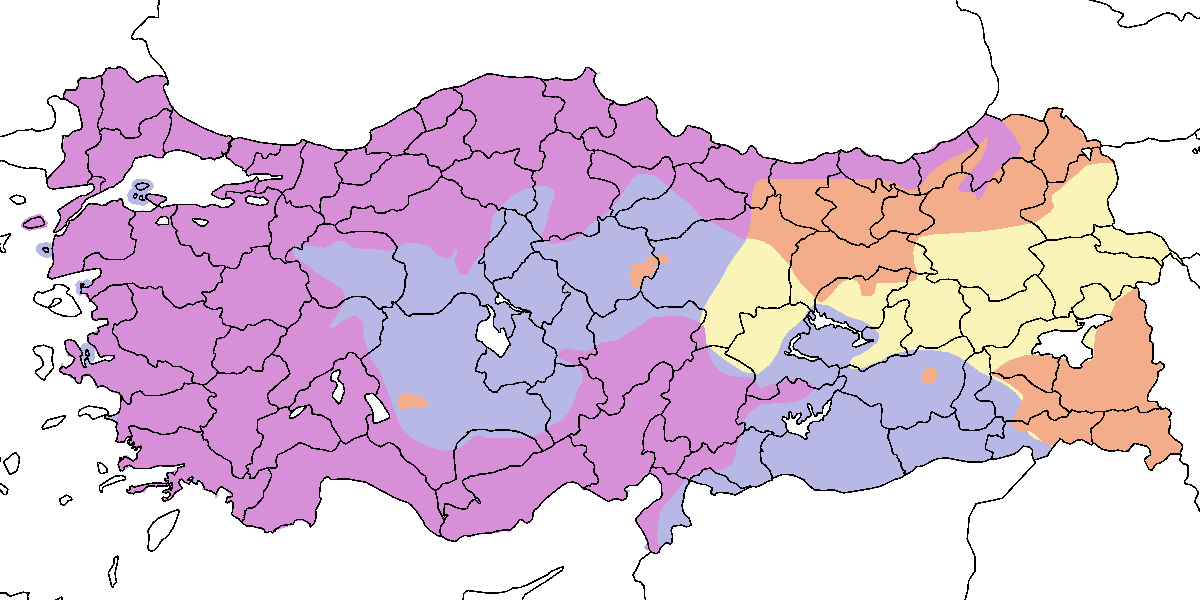
\includegraphics[keepaspectratio]{images/harita_Fringilla coelebs.png}}

\textbf{Üreme}

\textbf{Yuvalama alanı:} Plantasyonlar, zeytinlikler, meyve bahçeleri ve
yaygın olarak engebeli arazideki ibreli ormanlar da dâhil olmak üzere
her türlü ormanlık alanda ürer. Marmara Bölgesi'nde en yüksek üreme
yoğunluğu Uludağ'da 1100--1400 m arasındaki karaçam (\emph{Pinus nigra})
ormanında tespit edilmiştir (Jetz, 1995). Kocaçay Deltası'nda alüvyal
ormanda 31 hektarlık bir alanda hektarda 1,3 çift, çevredeki yaprak
döken ormanda ise daha yüksek yoğunluk belirlenmiştir (Ertan, 1996).
Kızılırmak Deltası'nda 1992 yılında ortalama yoğunluk 100 hektarda 15
savunulan alan olarak kaydedilmiştir (Hustings \& Dijk, 1994).\\
\textbf{Yuvası:} Muntazam ve derin bir kâse şeklindedir. Yosun, liken,
ot, kök ve tüylerle örülür, örümcek ağlarıyla sarılır ve içi tüy, yün ve
bitkisel havla astarlanır.\\
\textbf{Yumurta sayısı:} Türkiye'de az sayıda üreme kaydı vardır. İki
yuvada dörder yumurta ve iki yuvada dört ve beş yavru kaydedilmiştir.\\
\textbf{Üreme dönemi:} \textbf{MAR:} 25 Haziran 1973'te Üvecik'te bir
erişkin tüylenmiş bir yavruyu beslerken, 26 Haziran'da Paşaköy
çevresinde başka bir erişkin yuva materyali taşırken gözlenmiştir.
\textbf{KAD.} 1 Haziran 1992'de Kızılırmak Deltası'nda ve 9 Haziran
1975'te Boyabat'ın kuzeyinde birer erişkinin yiyecek taşıdığı
kaydedilmiştir (Hustings \& Dijk, 1994). \textbf{AKD:} 11 Mayıs 2003'te
Ağla'da genç bir çamda, yerden 2 m yüksekteki yuvada yaklaşık 3--4
günlük dört yavru bulunmuş ve ilk yumurtlamanın 23 Nisan civarında
gerçekleştiği tahmin edilmiştir. 28 Nisan 1967'de Akseki'de ibreli bir
ormanda en yaygın tür olarak gözlenmiş ve dört yumurtalı bir yuva
kaydedilmiştir. 19 Nisan 2004'te aynı bölgede, bir köknarın 3--4 m
yüksekliğinde tamamlanmamış iki yuva bulunmuştur. 12 Mayıs 2005'te
Uzuncaburç'ta beş yavrulu bir yuva ve 13 Mayıs'ta Mut'ta yavrulu başka
bir yuva kaydedilmiştir. 27 Mayıs 1999'da Eğirdir'de tüylenmiş yavrusunu
besleyen bir çift gözlenmiştir. \textbf{İÇA:} 26 Nisan 1983'te
Kızılcahamam'da dört yumurtalı bir yuva bulunmuş (Barış \emph{vd.},
1984) ve 25 Mayıs 1992'de henüz uçamayan tüylenmiş bir yavru
gözlenmiştir.

\textbf{Alttürler ve Sınıflandırma}

İspinoz taksonomisinin karmaşık olduğu ve örneklerin eksikliği nedeniyle
konunun belirsizliği bilinmektedir. Trakya'da \emph{coelebs} alttürü,
Güney Marmara, Karadeniz Bölgesi, İç Anadolu ve Doğu Anadolu'nun
kuzeyinde \emph{caucasica} alttürü bulunur; bu takson daha sonra
\emph{transcaspia}'nın sinonimi olarak kabul edilmiştir. Doğu
Anadolu'nun güneyi, Güneydoğu Anadolu ve Hatay'daki bireyler geçici
olarak \emph{syriaca} alttürüne dahil edilebilir. Güney Ege, Toroslar ve
Akdeniz kıyılarındaki bireyler ise, Girit Adası'ndaki bireylerde de
görüldüğü üzere \emph{schiebeli} ile \emph{syriaca} arasında geçiş formu
olabilir. Ayrıca, Kırım ve çevresinde bulunan \emph{solomkoi} alttürünün
Türkiye'de kışlama ihtimali de vardır. Roselaar, alttürler arasında
yalnızca çok hafif farklar bulunduğunu, bu farkların da genellikle
tüylerin yıpranması ve solması nedeniyle ayırt edilemediğini belirtmiş
ve ispinoz taksonomisinin sorunlu olduğunu vurgulamıştır (Roselaar,
1995).

\section{Dağ İspinozu}\label{daux11f-ispinozu}

\emph{Fringilla montifringilla}, Brambling

\textbf{\emph{Yaygın olarak nispeten çok sayıda bulunan kış konuğudur.}}

Ülkenin hemen her yerinde genellikle seyrek, ara sıra ve lokal olarak
kalabalık sürüler hâlinde görülen bir kış konuğudur. Trakya, Batı ve
Orta Anadolu'nun birçok yerinde kışlar; en yoğun olarak Kuzey, Batı ve
İç Anadolu bölgelerinde görülür. Doğu Anadolu'dan az sayıda kayıt vardır
ancak Malatya'da düzenli olarak kışladığı bilinmektedir. Güneydoğu
Anadolu'da ise düzensiz olarak gözlendiği tahmin edilmektedir.

Göç, mart sonunda başlar ve bu dönemde orta ve güney bölgelerdeki
bireylerin çoğu alanı terk etmiş olur; nadiren nisan ayına kadar
kalanlar da görülür. En geç kayıt 21 Nisan tarihindedir. Türün yaz
aylarında kalması çok nadirdir; bununla ilgili bilinen tek kayıt,
Erzurum'da haziran başına kadar kalan bir bireye aittir (McGregor,
1917). Sonbahar'da Eylül sonu ile kasım sonu arasında genellikle
İstanbul Boğazı, Trakya ve Kuzeydoğu Anadolu'ya ulaşır.

Bazı yıllarda yüksek sayılara ulaşır; örneğin 1966--67 ve 1988--89
kışlarında 1000'i aşan sürüler sıkça kaydedilmiştir. 1976 yılının
başında İç Anadolu'da istisnai yoğunlukta gözlenmiştir. 1500 metreye
kadar olan her türlü habitatta kaydedilmiştir.

\pandocbounded{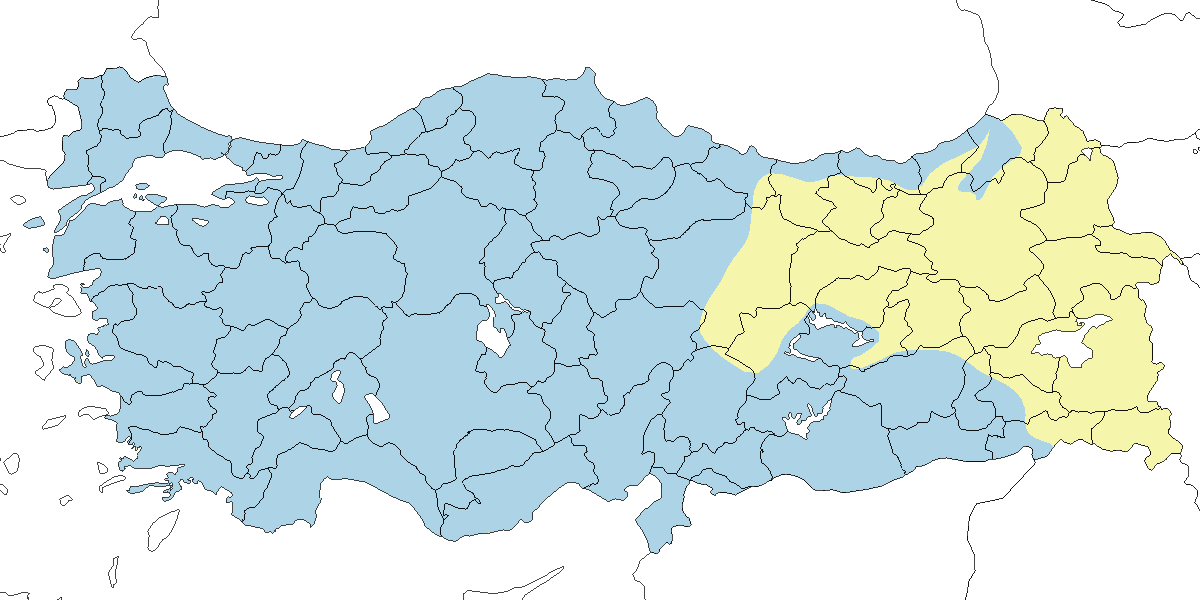
\includegraphics[keepaspectratio]{images/harita_Fringilla montifringilla.png}}

\textbf{Üreme}

Türkiye'de yuvalamaz. Kuzey Avrupa ve Asya'da yuvalar.

\textbf{Alttürler ve Sınıflandırma}

Monotipik bir türdür.

\section{Kocabaş}\label{kocabaux15f}

\emph{Coccothraustes coccothraustes}, Hawfinch

\textbf{\emph{Nispeten lokal olarak az sayıda bulunan yerli ve kış
konuğudur.}}

Marmara, Karadeniz Bölgesi'nin batısı ve İç Anadolu'nun kuzeyinde
yaygındır. Trakya'da yer yer çok bol olabilir. Güney Toroslar'da ürediği
gözlenmiş (Danford, 1877-78), bu bilgiyi güncel iki kayıt
desteklemiştir: Toroslar'ın doğusundan temmuz ayına (Roselaar, 1995) ve
mayıs ortasında Mut'un doğusundan gözlenmiştir. Doğu Anadolu da uygun
habitatlarda temmuzda Trabzon'da ve ağustosta Tunceli'de kaydedilmiştir
(Helbig, 1984).

Ekim ayından itibaren tüm ülkede geçit sırasında kaydedilir; İstanbul
Boğazı ve Borçka gibi göç izleme noktalarında nispeten az sayıda
gözlenir. Trakya, Batı ve Orta Anadolu'nun çeşitli bölgelerinde kışlar.
Kış kayıtlarının büyük bölümü Marmara, Ege ve Akdeniz'in kıyı
kesimlerinden gelmekte ve bu bölgelerdeki ormanlık alanlarda yer yer çok
sayıda birey görülebilmektedir. Bu dönemde İç Anadolu'da da kaydedilmiş,
istisnai olarak Doğu Anadolu'da da gözlenmiştir. Bu bölgelerde irtifa
göçü yaptığı düşünülmektedir.

\pandocbounded{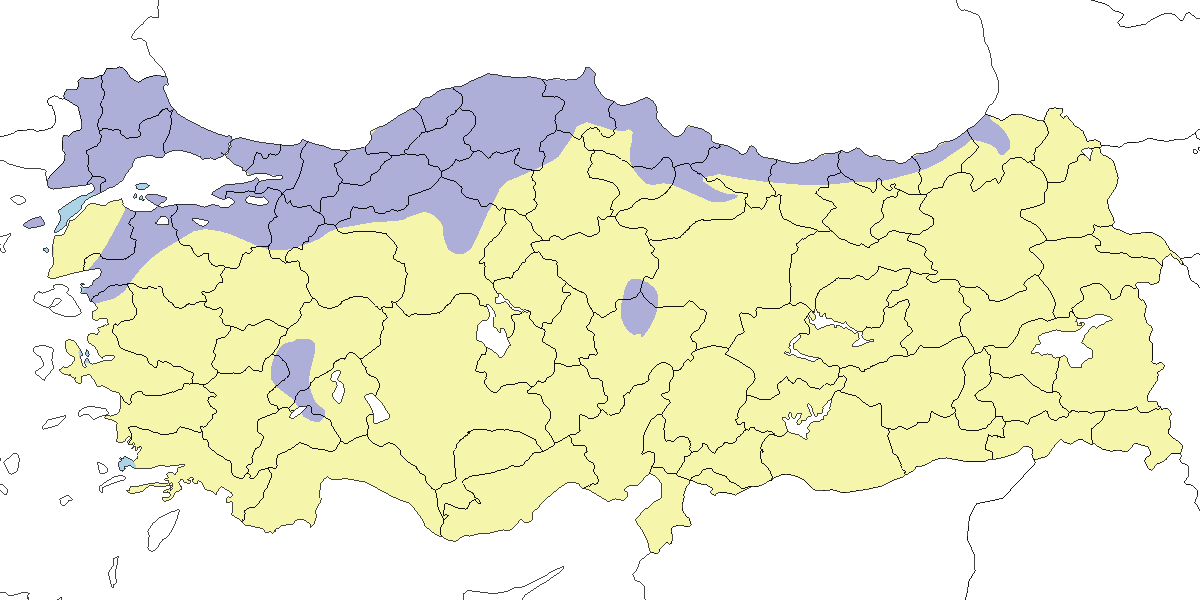
\includegraphics[keepaspectratio]{images/harita_Coccothraustes coccothraustes.png}}

\textbf{Üreme}

\textbf{Yuvalama alanı:} Çoğunlukla yaşlı ve yaprak döken ormanlarda,
Marmara'da özellikle Trakya'da, Karadeniz Bölgesi'nin batısında ve
nadiren İç Anadolu'da ürer.\\
\textbf{Yuvası:} Türkiye'de yuva ile ilgili doğrudan bilgi
yayımlanmamıştır. Diğer bölgelerde yuva genellikle bir ağaca ve 4 m'den
yükseğe kurulur. Dal, kök ve likenlerden yapılan kâse şeklindeki yuva,
daha ince kökler, bitki lifleri ve kıllarla astarlanır.\\
\textbf{Yumurta sayısı:} Türkiye'de veri yoktur. Diğer bölgelerde olağan
yumurta sayısı 4--5'tir.\\
\textbf{Üreme dönemi:} \textbf{MAR:} 14 Mayıs 1970'te Belgrad Ormanı'nda
bir çift, 18--29 Haziran 1973'te ise yiyecek taşıyan erişkinler
gözlenmiştir. 21 Temmuz 1973'te Kavakköy'de yiyecek taşıyan erişkinler
ve 17--19 Haziran 1973'te İstanbul Bebek'te yeni tüylenmiş yavruyu
besleyen bir erişkin kaydedilmiştir. Bu son gözlem yumurtlamanın mayıs
ortasında olduğunu göstermektedir. \textbf{KAD.} 9 Haziran 1978'de
Alaplı'da yuva malzemesi taşıyan bir erişkin gözlenmiştir. Bu kayıt
muhtemelen telafi kuluçkasına veya ikinci kuluçkaya işaret etmektedir.
İki kez kuluçkaya yatma yayılış alanının diğer bölgelerinde de zaman
zaman gözlenmektedir. \textbf{İÇA:} 5 Haziran 1996'da Kızılcahamam'da
yiyecek taşıyan bir erişkin gözlenmiştir.

\textbf{Alttürler ve Sınıflandırma}

Doğu ve Güney Balkanlar'daki kuşların nominat \emph{coccothraustes} ile
Güney Kafkasya'daki \emph{nigricans} arasında yer alan bir klinal
varyasyonun parçası olduğu düşünülmektedir (Roselaar, 1995). Türkiye'nin
batısındaki bireylerin \emph{nominat} alttür altında değerlendirilmesi
güvenli bir yaklaşımdır. Doğu Anadolu'dan örnekler toplanmış ancak
sonradan kaybolmuştur; dolayısıyla \emph{nigricans} alttürünün
Türkiye'nin kuzeydoğusuna kadar ulaşıp ulaşmadığı kesin olarak
söylenemez. Kayıt eksikliği nedeniyle Karadeniz Bölgesi'de olmadığı
düşünülerek klinal varyasyonun geçerli olmadığı öne sürülmüştür
(Roselaar, 1995), ancak bu durumun gözlem eksikliğinden
kaynaklandığından dolayı klinal bir varyasyon varsayımı mantıklı
görünmektedir.

\section{Çütre}\label{uxe7uxfctre}

\emph{Carpodacus erythrinus}, Common Rosefinch

\textbf{\emph{Yaygın olarak nispeten çok sayıda bulunan yaz konuğudur.}}

Karadeniz Bölgesi'nde en bol ve yaygın olarak bulunur. İç Anadolu'nun
kuzeyinde oldukça lokal, ülkenin kuzeyi boyunca yayılış gösterir ve
batıda Uludağ'a kadar ulaşır. Trakya'da yalnızca Bulgaristan sınırına
yakın tek bir kayıt vardır; burada düzenli olarak ürediği
düşünülmemektedir. Ülkenin batısına doğru yayılımının geçen yüzyılın
ortalarında gerçekleştiği öne sürülmüştür (Kumerloeve, 1975c, 1966a).
Doğu Anadolu'da, uygun habitatın bulunduğu yerlerde güneyde Hakkâri
Dağları'na kadar yayılır, ancak bu bölgede nispeten lokaldir. İç
Anadolu'da örneğin Sultansazlığı'nda birkaç kez üreme tespit edilmiştir.
Akdeniz Bölgesi'nin kuzeyinde, haziran başında bir defa kaydedilmiştir
(Deppe, 1990). Güneydoğu Anadolu'da da baharın sonuna doğru uygun
habitatlarda rastlanmıştır, ancak üreme henüz doğrulanmamıştır.

Çoğunlukla nisan sonundan itibaren gelir, ancak en kuzeydeki üreme
alanlarına varışı yaklaşık üç hafta gecikebilir. En erken 2 Nisan'da
kaydedilmiştir. Üreme alanlarından ayrılış ağustosun ikinci yarısında
başlar, eylül boyunca sürer. Doğu Anadolu'da 23 Ağustos'ta geçişte, en
geç 3 Ekim'de gözlenmiştir. Eylül sonu ve ekim başında göç tamamlanır;
en geç 12 Ekim'de kaydedilmiştir. Geçit sırasında daha yaygındır ve
batıda çok nadir de olsa ülkenin her bölgesinde rastlanabilir. Kışlaması
ise istisnadır; yalnızca bir defa 26 Aralık 2004'te Göksu Deltası'nda
kaydedilmiştir.

\pandocbounded{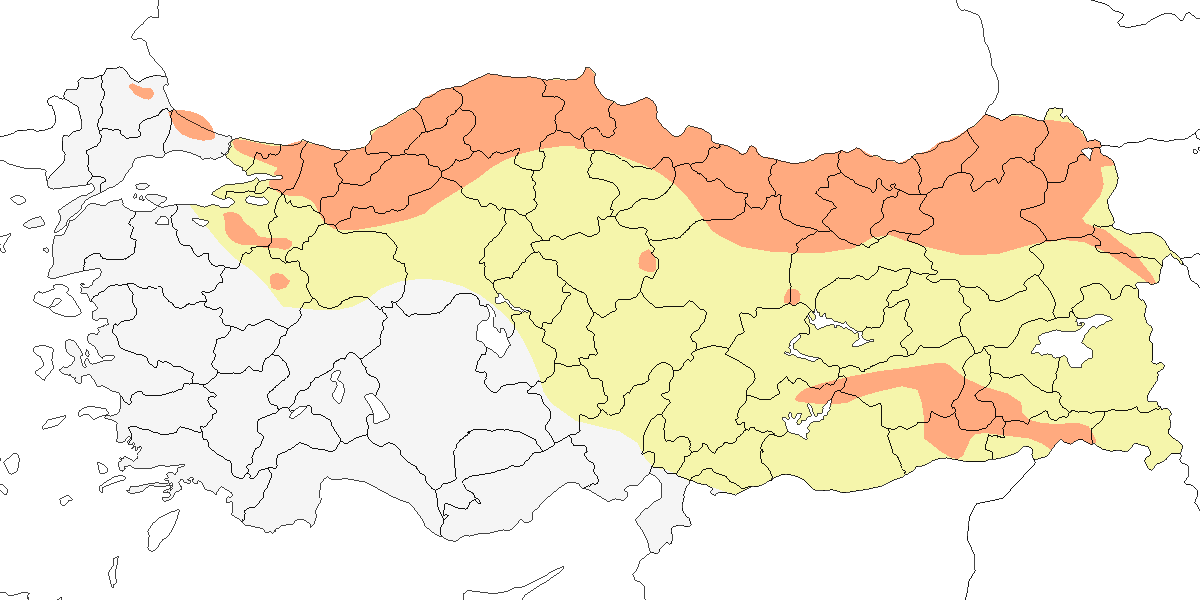
\includegraphics[keepaspectratio]{images/harita_Carpodacus erythrinus.png}}

\textbf{Üreme}

\textbf{Yuvalama alanı:} Üreme habitatı karışık ormanlar, tıraşlanmış
veya yeniden dikilmiş ormanlar ve bahçeler olup 400 m'den Uludağ'da en
azından 2700 m'ye kadar orta veya yüksek irtifada bulunur. Seyrek
çalılar, çitler ve bodur ağaçların bulunduğu çayırlarda, alt örtüsü
bulunan seyrek ağaçlı ormanlar, baltalıklar, bahçeler ve tarım
arazilerindeki çalılıklarda ürer. Nemli ve içine girilemeyen
çalılıklarda, göl ve nehir kenarındaki söğütlüklerde de sıklıkla
bulunur.\\
\textbf{Yuvası:} Yuvasını bir çalıya veya genç bir ağaca, yerden 0,3--2
m yüksekliğe yapar. Bitki kökleri ve otlardan oluşan gevşek bir kâse
şeklindeki yuvasını kökler ve kıllarla astarlar.\\
\textbf{Yumurta sayısı:} Türkiye'de iki yuvada 4, altı yuvada 5 yumurta
kaydedilmiştir.\\
\textbf{Üreme dönemi:} \textbf{KAD.} Yeniçağa Gölü'nde yuva yapımı 20
Mayıs 1992'de başlamış, 29 Mayıs'ta bile henüz tamamlanmamıştır. 20
Haziran'da yuva yapan iki çift, 22 Haziran'da tek yumurtalı bir yuva ve
20 Haziran'da iki yumurtalı yuvalar gözlenmiştir; bu tarihlerde çevrede
beş yumurtalı tamamlanmış kuluçkalar da kaydedilmiştir. Üç yuvadan
ikisinde dört, birinde beş yumurta bulunmuştur. 27 Mayıs 1992'de Abant
Gölü'nde ve 30 Haziran 1977'de İsmetpaşa'da yuva yapımı gözlenmiştir. 9
Temmuz 1970'te Kızılırmak Deltası'nda tüylenmiş yavrular, 11 Haziran
2004'te Yoncalı'da tek yumurtalı bir yuva, 15 Haziran'da aynı yuvada beş
yumurta, ayrıca yine 15 Haziran'da başka bir yuvada beş yumurta
kaydedilmiştir. Uludağ'da en erken ötüş 11 Mayıs 1993'te duyulmuştur.
\textbf{DOA:} Sarıcan'da 16 Haziran 2004'te yuva yapımına uygun ama boş
iki yuva, 25 Haziran'da ise iki yumurtalı bir yuva kaydedilmiştir. Geç
yuvaladığı bariz bir türdür. 9 Haziran 1982'de Sultansazlığı'nda
kaydedilen üç yavruyla birlikte uçan çiftin kaydı istisnai derece
erkendir.

\textbf{Alttürler ve Sınıflandırma}

Kuzey ve kuzeydoğu Anadolu'da \emph{kubanensis} alttürü bulunur. En uç
kuzeydoğuda ise \emph{erythrinus} nominat alttürünün görülme ihtimali
vardır (Roselaar, 1995). \emph{Kubanensis}, Orta Avrupa ile daha
doğudaki popülasyonlar arasında taksonomik bir köprü olarak
değerlendirilir (Helb \emph{vd.}, 1995).

\section{Şakrak}\label{ux15fakrak}

\emph{Pyrrhula pyrrhula}, Eurasian Bullfinch

\textbf{\emph{Lokal ve seyrek yerli ve yarı göçmendir.}}

Karadeniz Bölgesi'nde, 2500 m'ye kadar olan yükseltilerde yaygındır.
Marmara ve Kuzey Ege'de ise dağlık ibreli ve yer yer karışık ormanlarda
çok yerel olarak görülür.

İç Anadolu'nun kuzey sınırında, kış aylarında düzenli olarak gözlenir.
Kuzeydoğu Toroslar'ın en uç kesimlerinden haziran ve temmuz aylarına ait
kayıtlar mevcuttur. Ekim ile şubat arasında, batı ve orta bölgelerde
---özellikle kıyı kesimlerinde--- daha yaygındır ve küçük gruplar
hâlinde görülür. Ankara'da mayıs sonuna kadar kalmıştır. Aynı dönemde
istisnai olarak Birecik'te de kaydedilmiştir.

\pandocbounded{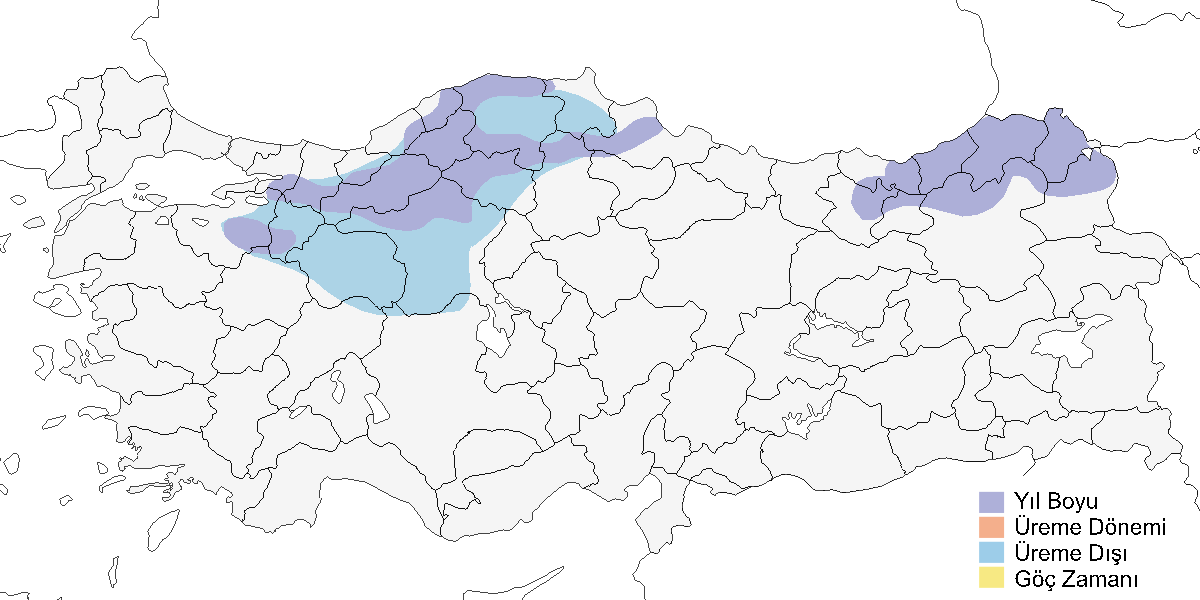
\includegraphics[keepaspectratio]{images/harita_Pyrrhula pyrrhula.png}}

\textbf{Üreme}

\textbf{Yuvalama alanı:} Çoğunlukla Karadeniz Bölgesi'nde 900 m'nin
üstündeki sık ibreli ve karışık ormanlarda ürer.\\
\textbf{Yuvası:} Türkiye'de yuva ile ilgili kayıt bulunmamaktadır. Diğer
bölgelerde yuva genellikle bir çalı veya genç bir ağacın üzerine, yerden
1--2 m yükseğe yapılır. Sığ yapıdaki yuva, ince dallar, yosun ve
likenlerle örülür; kökler ve kıllarla astarlanır.\\
\textbf{Yumurta sayısı:} Türkiye'de veri yoktur. Diğer bölgelerde olağan
yumurta sayısı 4--5'tir.\\
\textbf{Üreme dönemi:} \textbf{KAR:} 9 Haziran 1975'te Boyabat'ta
tüylenmiş yavrularını besleyen bir çift gözlenmiştir. Bu kuşların
habitatı, yaklaşık 1300 m yükseklikte, arada tarım arazileri, birkaç
yapraklı ağaç ve çalı bulunan çamlarla kaplı kireçtaşı tepelerdir. 25
Ağustos 2000'de Sivrikaya'da sık orman içinde yavrular, 31 Ağustos
1973'te İkizdere'de iki yavru gözlenmiştir. Bu kayıtlar büyük olasılıkla
ikinci kuluçkaya aittir ve çift kuluçka, bu enlemdeki diğer bölgelerde
de yaygındır.

\textbf{Alttürler ve Sınıflandırma}

Anadolu'da üreyen bireyler \emph{rossikowi} alttürü olarak
tanımlanmıştır. Batı Karadeniz için Karadere, Bolu Dağı, Abant Gölü ve
Ilgaz Dağları'nda toplanan örnekler ile morfolojik ölçüm verilerine
dayanarak \emph{paphlagoniae} adlı bir alttür tanımlanmıştır (Roselaar,
1995). Ancak bu üreme bölgesinden çok sayıda örnek incelenmiş ve
taksonomik düzeyde tanımlanmasını destekleyecek argümanların zayıf
olduğu belirtilmiştir (Kirwan, 2006). Bu nedenle \emph{paphlagoniae}
taksonunu \emph{rossikowi}'nin bir sinonimi olarak değerlendirmek daha
uygundur. Tring Doğa Tarihi Müzesi, Manchester Müzesi ve Sofya Ulusal
Doğa Tarihi Müzesi'ndeki Avrupa ve Batı Asya'dan toplanan örnekler
incelendiğinde, pek çok coğrafi tanımın geçerli olmadığı
düşünülmektedir. Örneğin, \emph{germanica} ve \emph{europaea}
alttürlerini uzun bir örnek serisiyle bile birbirinden kesin biçimde
ayırmak mümkün değildir; bu nedenle \emph{germanica} alttürü bir sinonim
kabul edilmiştir. Ayrıca, nominat \emph{pyrrhula} alttürünün Türkiye'ye
kış aylarında ulaşması olasıdır. Nitekim 2004 sonbaharındaki bir akın
sırasında Bulgaristan'da bu tipe benzeyen kuşların gözlendiği
bildirilmiştir (Pennington \& Meek, 2006).

\section{Alamecek}\label{alamecek}

\emph{Rhodopechys sanguineus}, Crimson-winged Finch

\textbf{\emph{Lokal olarak az sayıda bulunan yerli ve irtifa
göçmenidir.}}

Yüksek ve nispeten kurak dağlık alanlarda bulunur. Doğu Karadeniz'in
doğusu ve iç kesimleri, Doğu Toroslar ve etekleri ile İç Anadolu'da Tuz
Gölü'nün doğusundaki dağlık alanlarda yer yer boldur. Genellikle seyrek
bitkili kayalık yamaçları tercih eder. En azından Ağrı Dağı'nda 4200
m'ye kadar, Doğu Anadolu'da sıkça 1600 m'nin üzerindeki tarım
arazilerinde ve daha batıda düzenli olarak en az 900 m'ye kadar olan
nispeten alçak bölgelerde ürer. Üreme genellikle nisan ayında başlar,
doğuda ise bu dönem muhtemelen biraz daha geçtir. Eber Gölü çevresinden
gelen, biri Mayıs 1967'de diğeri 1992'de kaydedilmiş iki üreme dönemi
kaydı, ana yayılış alanının sınırındandır. Buna ek olarak, daha güney ve
batıdan da üreme dönemi kayıtları vardır.

Kış aylarında İç Anadolu'nun bozkırlarında nadiren görülür. Ege'de tek
tük, Marmara'da ise istisnai olarak Biga'da kaydedilmiştir (OST, 1969).
Ancak kışın çoğunlukla Doğu Anadolu'da, 2000 m'ye kadar olan
yüksekliklerde kalır.

\pandocbounded{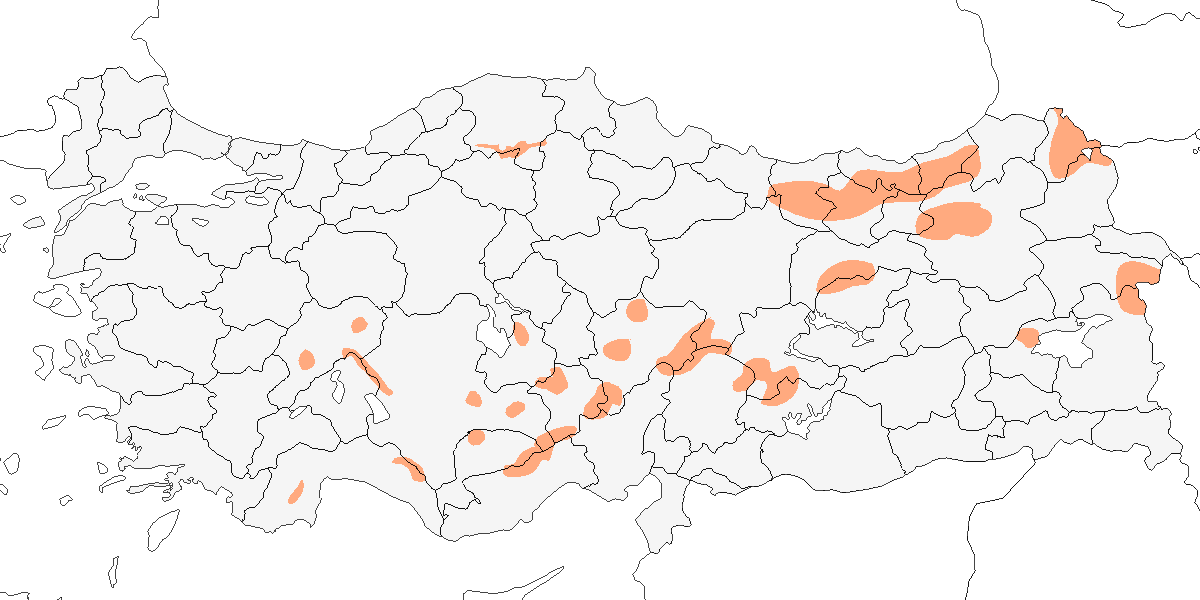
\includegraphics[keepaspectratio]{images/harita_Rhodopechys sanguineus.png}}

\textbf{Üreme}

\textbf{Yuvalama alanı:} Seyrek bitkili, çıplak topraklı ve taşlı dik
yamaçlarda, ara sıra bodur ağaçlar arasında ve lav yataklarında,
neredeyse tamamen bitkisiz alanlarda ürer. Ayrıca, Tuz Gölü'nün
doğusunda bağlık ve dağınık ağaçlı yamaçlar ile kayalık vadiler ve
seyrek, bodur ağaçlı düz açık arazilerde de bulunur (Roselaar, 1995).\\
\textbf{Yuvası:} Meke Tuzlası'nda (Konya) 1100 m rakımda, 45° eğimli
küllü yamaçlarda ve yaklaşık 40 × 50 × 20 cm boyutlarındaki lav
plakalarının altında, girişi doğuya bakan yuvalar bulunmuştur (Lehmann
\& Mertens, 1969). Aynı bölgede lav plakalarının altına ek olarak alçak
adaçayı (Salvia) öbeklerinde de yuvalar tespit edilmiştir (McNeile,
1950, 1951, 1954, 1967, 1968, 1970, 1972, 1973). Yuvalar kuru bitki
gövdelerinden kabaca örülür ve ince ot ile bitkisel liflerle
astarlanır.\\
\textbf{Yumurta sayısı:} Türkiye'de 5 yumurtalı üç yuva, 5 yavrulu bir
yuva kaydedilmiştir.\\
\textbf{Üreme dönemi:} Nisan ayında yumurta koymaya başlar, yavrular
ağustos ayına kadar görülebilir. Yayılış bölgesinin diğer kısımlarında
da yılda iki kez kuluçkaya yatar. \textbf{AKD:} 13 Nisan 1994'te yuva
yapımı ve kur davranışı gösteren çiftler gözlenmiş, 19 Temmuz 1971'de
Torosdağ'da yeni tüylenmiş yavrularını besleyen erişkinler
kaydedilmiştir. \textbf{İÇA:} 6 Mayıs 1968'de Meke Tuzlası'nda biri dört
yavru ve bir yumurtalı, biri yumurtalı, diğeri uçmaya hazır yavrulu
olmak üzere üç yuva bulunmuştur. Yumurtlamanın sırasıyla 17, 20 ve
yaklaşık 1 Nisan'da gerçekleştiği tahmin edilmiştir (Lehmann \& Mertens,
1969). 30 Nisan--9 Mayıs 1970 arasında yumurtalı dört yuva tespit
edilmiş, 20 Nisan 1970'te beş ve dört yumurtalı iki yuva kaydedilmiş,
ertesi gün ikinci yuvaya bir yumurta daha eklenerek beşlenmiştir. 22
Nisan'da beş yumurtalı ve tek yumurtalı iki yuva bulunmuş, 21 Nisan
1973'te biri boş ancak yumurtlamaya hazır, diğer ikisi ise yumurtalı üç
yuva kaydedilmiştir (McNeile, 1950, 1951, 1954, 1967, 1968, 1970, 1972,
1973). 4 Mayıs 2005'te bir kayanın altında dört yumurtalı bir yuva
bulunmuş, yumurtlamanın henüz tamamlanmadığı anlaşılmıştır. 9 Mayıs
1967'de Sultan Dağları'nda çiftleşme, 19 Haziran 1996'da Karadağ'da
tüylenmiş bir yavru gözlenmiştir (Kirwan, 1998). 24 Temmuz 1971'de üç
tüylenmiş yavru, 25 Haziran 1977'de ise en az üç çiftin yavrularına
yiyecek taşıdığı ve bir çiftin iki tüylenmiş yavrusunu beslediği
kaydedilmiştir (Schubert, 1979). \textbf{DOA:} 2 Haziran 1969'da
Görentaş yakınlarında bir erişkinin yuva malzemesi taşıdığı, 11 Mayıs
1992'de Van yakınında bir çiftin yuva üstünde olduğu gözlenmiştir. 1966
yazında Temmuz sonu ile Ağustos başında Süphan Dağı'nda birkaç aile
grubu kaydedilmiştir. Erzurum yakınlarında bir yıl içinde iki kez
ürediğine dair gözlemler vardır. 20 Ağustos gibi geç tarihlerde uçabilen
yavruların bulunduğu aile grupları bunun kanıtı olarak sunulmuştur
(McGregor, 1917).

\textbf{Alttürler ve Sınıflandırma}

Tip örneği Erzurum'dan toplanmıştır; dolayısıyla nominat alttür bulunur.
Kuzeydoğu Afrika'da Atlas Dağlarındaki \emph{alienus} alttürünün bütün
giysilerindeki farklılıklar ve morfolojik özellikleri dikkate alınarak
iki allopatrik tür olduğu öner sürülmüş (Kirwan \& Shirihai, 2006), bu
öneri kabul görmemiştir. Bilimsel ismin doğru yazılışına dikkat ediniz
(David \& Gosselin, 2002b). Cins düzeyinde taksonomik tartışmalar için
doğu alameceğine bakınız.

\section{Küçük Alamecek}\label{kuxfcuxe7uxfck-alamecek}

\emph{Bucanetes githagineus}, Trumpeter Finch

\textbf{\emph{Çok lokal ve az sayıda yaz göçmenidir.}}

Nisan sonu ile ağustos ortası arasında görülen nadir bir yaz göçmenidir.
Güneydoğu Anadolu'da ürediği ispatlanmıştır (Martins, 1989). Yayılışı
düzenli bir göçten ziyade, göçebe hareketlerle açıklanabilir. Kuzeyde
Doğubayazıt'a kadar, güneyde ise Akdeniz Bölgesi sınırına kadar
ulaşabilir.

Kayıtlar şöyledir: 24 Mayıs 1974'te Iğdır Tuzluca'da iki erkek ve iki
dişi; aynı tarihlerde Tuzluca ile Kağızman arasında çok sayıda birey; 6
Haziran 1987'de Gaziler (Tuzluca-Kağızman) yakınlarında altı birey; 13
Haziran 1977'de Nemrut Dağı'nda (Tatvan) muhtemel bir birey (Krieger,
1988); 28 Haziran 1977'de Gaziantep Yeşilce'nin güneyinde beşi genç yedi
birey ve aynı bölgede Haziran 1996, Mayıs 1997, 1999 ve 2000'de tekrar
gözlemler (Kirwan \& Martins, 2000; Kirwan \emph{vd.}, 2003); 10 Mayıs
1979'da Alanya-Manavgat arasında bir çift; 17 Ağustos 1987'de Tatvan
Nemrut Dağı'nda bir erkek (Krieger, 1988); 24 Nisan 1988'de
Silifke--Mersin arasında bir birey; 17 Mayıs 1989'da Birecik--Cizre
arasında bir birey; 16--17 Haziran 1990'da Birecik'te bir birey (Kirwan
\& Martins, 1994); 17 Mayıs 1992'de yine Birecik'te üç birey (Kirwan \&
Martins, 2000); 8 Temmuz 1997'de Doğubayazıt'ta bir birey; 31 Temmuz--2
Ağustos 1998'de aynı bölgede iki birey (Kirwan, Bechtolsheim \& Willig,
2000); 24 Haziran 2004'te iki genç (Balmer \& Betton, 2005a); 10 Ağustos
1998'de Tatvan Nemrut Dağı'nda üç dişi veya genç birey; 29 Nisan 1999'da
Diyarbakır Çınar--Göksu Barajı'nda iki birey (Karakaş \& Kılıç, 2002);
13 Haziran 1999'da Göksu Deltası'nda iki erkek (Kirwan \emph{vd.},
2003); 30 Mayıs 2005'te Erciş'in batısında Van Gölü kıyısında bir çift;
26 Mayıs 2005'te Pervari'de öten bir erkek; 1 Nisan 2008'de Mileyha'da
bir birey.

Küçük Alamecek ile Doğu Alameceği'nin Tuzluca ve Doğubayazıt çevresinde
birlikte kaydedilmesi bu türlerin karıştırılabileceği ihtimalini doğursa
da, gözlemler ayrıntılı tariflerle desteklenmiştir. Azerbaycan'da her
iki türün aynı bölgede yan yana ürediği de belgelenmiştir (Clement,
Harris \& Davis, 1993). İlk kayıt iddiası (Dement'ev \& Gladkov,
1951/54) belgelenmediği için geçerli sayılmamış ve reddedilmiştir
(Kumerloeve, 1961). 1974'ten bu yana 22'den fazla güvenilir ve ayrıntılı
kayıt yayımlanmıştır.

\pandocbounded{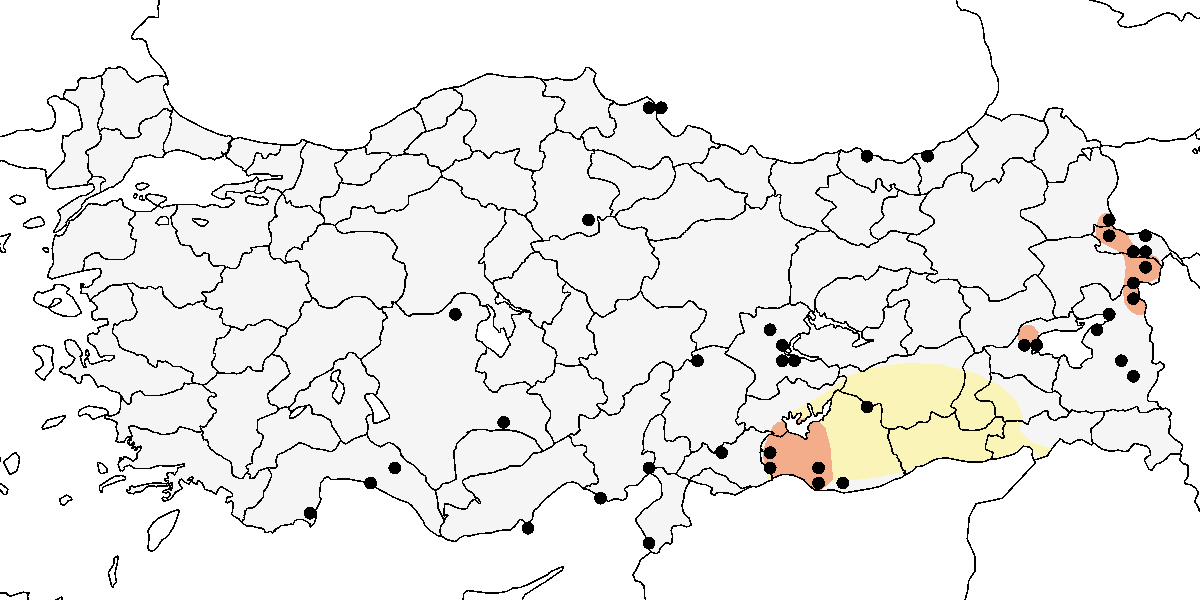
\includegraphics[keepaspectratio]{images/harita_Bucanetes githagineus.png}}

\textbf{Üreme}

\textbf{Yuvalama alanı:} Türkiye ve Ermenistan'da yayılış alanının kuzey
sınırında yer alır. Türkiye'de özellikle Doğubayazıt ve Gaziantep
çevresinde ürer. Diğer bölgelerde çölde kayalık alanlarda, alçak bir
yarda, kaya çatlağı ya da oyuklara; bazen duvarlara, teraslara ve eski
binalara yuva yapar. Yuvasını zaman zaman bir kayanın ya da alçak bir
çalının gölgesine kurabilir.\\
\textbf{Yuvası:} Kâse şeklindedir. Bitki kökleri, dallar ve otlardan
yapılır, içi kıl ve yünle astarlanır.\\
\textbf{Yumurta sayısı:} Türkiye'de doğrudan veri yoktur. Diğer
bölgelerde ortalama 4--6 yumurta bırakır.\\
\textbf{Üreme dönemi:} Diğer bölgelerde üreme mart ve nisanda başlar ve
yılda iki kez kuluçkaya yattığı bilinmektedir. \textbf{DOA}. 24 Haziran
2004'te Doğubayazıt'ta iki tüylenmiş yavru kaydedilmiştir (Balmer \&
Betton, 2005a). Temmuz 2006'da Doğubayazıt çevresinde bir yuva tespit
edilmiştir. Komşu Ermenistan'da 17 Nisan 1961'de Vedi yakınında üreyen
bir çift, 7 ve 31 Temmuz 1995'te çiftler ve bir genç birey, 4 Ağustos'ta
ise bir erişkin ve dört gençten oluşan bir aile grubu su içerken
gözlenmiştir (Adamian \& Klem, 1999). \textbf{GDA:} 28 Haziran 1977'de
Gaziantep yakınında beş yavru gözlenmiştir.

\textbf{Alttürler ve Sınıflandırma}

Türkiye'den toplanmış hiçbir örnek bulunmamaktadır. Ancak ülkede
gözlenen bireylerin güvenle \emph{crassirostris} alttürüne ait olduğu
söylenebilir (Roselaar, 1995). Taksonomik değerlendirme için Doğu
Alameceği altındaki tartışmalara bakınız.

\section{Doğu Alameceği}\label{doux11fu-alameceux11fi}

\emph{Bucanetes mongolicus}, Mongolian Finch

\textbf{\emph{Lokal olarak az sayıda bulunan yerli ve irtifa
göçmenidir.}}

Genellikle küçük sayılarda, Doğu Anadolu'nun en doğusunda bulunur.
Başlıca yayılış alanı Kars ve Van illerinin Ermenistan ve İran sınırına
yakın bölgeleri ile güneyde Hakkâri, doğuda ise Tunceli'deki Munzur
Dağları ve Sultanbaba Dağı'dır. Bu yayılış alanının dışındaki bölgelerde
tür irtifa göçmeni olarak görülmektedir (Clement \emph{vd.}, 1993). Doğu
Karadeniz'de sık ziyaret edilen Sivrikaya'da da gözlenmiştir. Güncel tüm
kayıtlar, 800--2700 m arasındaki kurak, yarı kurak ve kayalık dağlık
alanlardan bildirilmiştir; daha yüksek rakımlarda da bulunması
muhtemeldir. Genellikle alçak çalılıklar, otsu bitkiler ve açık
yamaçlarda görülür. Türkiye'den bildirilen yaklaşık 60 kayıt, hepsi 1977
sonrasına aittir ve en fazla 25 bireylik grupları kapsamaktadır (Kirwan,
1994, 2001; Kirwan \emph{vd.}, 2003).

Tarihi ancak yetersiz belgelenmiş bazı kayıtlar da mevcuttur. Mayıs 1911
ve 1912'de Nahçivan'daki Bulgan yakınlarında, bugünkü
Türkiye-Ermenistan-Azerbaycan sınır üçgenine yakın bölgelerde
gözlenmiştir (Bobrinskij, 1916). Ayrıca 1915 ilkbaharında Iğdır'ın
Tuzluca ilçesinde küçük bir sürü tespit edilmiştir (Beme, 1926). Türün,
Ermenistan'ın güneyinde büyük olasılıkla ürediği bilinmektedir (Beddard,
Ananian \& Finn, 2002; Ananian \& Busuttil, 2003). Bu erken dönem
kayıtlar bir zamanlar şüpheli kabul edilmişse de (Kumerloeve, 1961),
güncel bulgular ışığında değerleri yeniden anlaşılmıştır. Türün Türkiye
ve Batı Palearktik'teki durumu kapsamlı şekilde ele alınmıştır (Barthel
\emph{vd.}, 1992; Kirwan \& Konrad, 1995; Kirwan \& Gregory, 2005).

\pandocbounded{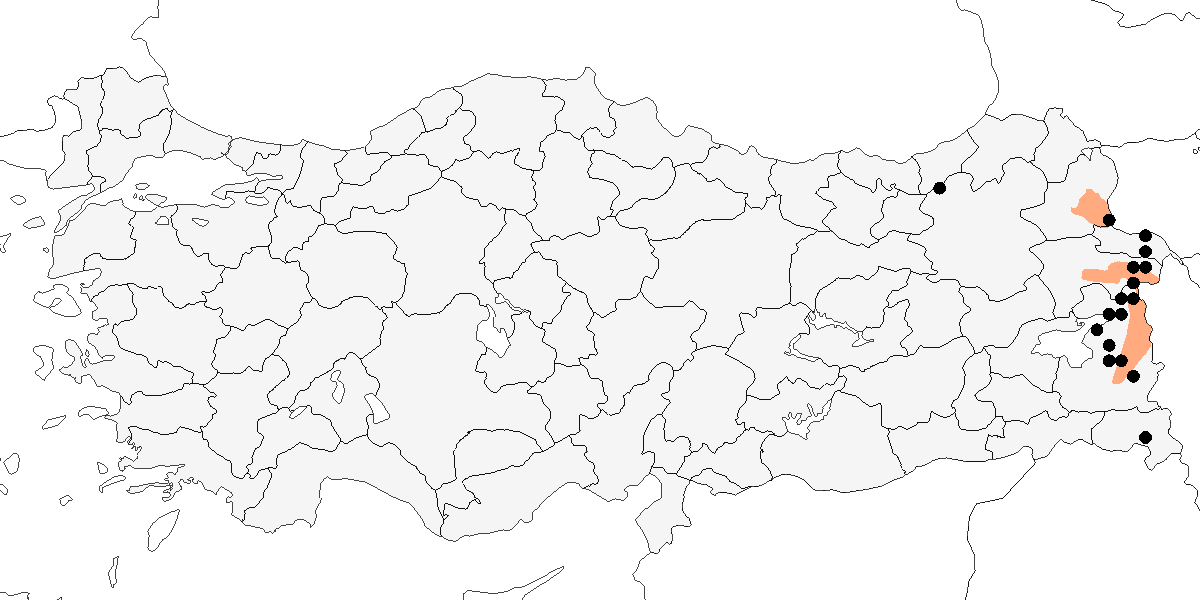
\includegraphics[keepaspectratio]{images/harita_Bucanetes mongolicus.png}}

\textbf{Üreme}

\textbf{Yuvalama alanı:} Kurak ve kayalık bölgelerde, taşlık çıplak
arazideki seyrek ve alçak çalılıklarda, genellikle nispeten yüksek ve
dik yamaçlarda ürer. Doğu Anadolu'da İshak Paşa Sarayı çevresinde seyrek
bitkili yamaçlarda, yar eteklerinde; Iğdır Tuzluca'da alçak otsu
bitkilerin ve yaklaşık 1 m yüksekliğindeki seyrek çalıların bulunduğu
iki kurak vadide gözlenmiştir. Geniş siyah lav düzlüklerinde, seyrek
vejetasyonlu alanlarda da bulunabilir.\\
\textbf{Yuvası:} Türkiye'den doğrudan kayıt yoktur. Diğer bölgelerde
yuva yerde, küçük bir çatlakta ya da oyukta veya üstten sarkan alçak bir
çalı ya da kayanın gölgesinde yer alır. Seyrek ve derin olmayan kâse
şeklindeki yuva, kuru ot kökleri ve yaprak şeritlerinden yapılır, kıl ve
yünle astarlanır.\\
\textbf{Yumurta sayısı:} Türkiye'de gözlem yoktur. Diğer bölgelerde
ortalama yumurta sayısı 3--5'tir.\\
\textbf{Üreme dönemi:} Haziran başında yumurta koyar. Yavrular haziran
sonu ve temmuz başı çıkar. Diğer bölgelerde olduğu gibi yılda bir kez
kuluçkaya yattığı tahmin edilmektedir. \textbf{DOA:} 17 Temmuz 1988 ve
21 Temmuz 1994'te İshak Paşa Sarayı çevresinde birçok genç, haziran 1996
başında çoğunlukla çiftler hâlinde 20--42 erişkin ve 9 Ağustos 2001'de
bir genci besleyen bir dişi kaydedilmiştir. 16 Temmuz 1990'da Çaldıran
Aşağı Mutlu'da bir çift iki yavruyu beslerken, 23 Haziran 2000'de
Doğubayazıt'ta bir yuvada üç yavru bulunmuş ve yumurtlamanın haziran
başında gerçekleştiği anlaşılmıştır. 28 Temmuz 2004'te Serpmetaş'ta bir
çift ve üç genç birey gözlenmiştir (Balmer \& Betton, 2005a). 23 Ağustos
1982'de Sultanbaba Dağı'nda genç bir birey kaydedilmiştir.

\textbf{Alttürler ve Sınıflandırma}

Monotipik bir türdür. Uzun süre boyunca tür düzeyinde tanınıp
tanınmaması ve hangi cinse ait olduğu tartışmalı olmuştur. Uzun süre
boyunca alamecek (\emph{Rhodopechys}) ve boz alamecek (\emph{Bucanetes
githagineus}), tek bir cins (\emph{Rhodopechys}) altında
değerlendirilmiştir (Vaurie, 1949; Cheng, 1987; Sibley \& Monroe, 1990;
Clement \emph{vd.}, 1993). Ancak bazı araştırmacılar dört türü
(\emph{Rhodopechys}, \emph{Bucanetes}, \emph{Eremopsaltria},
\emph{Rhodospiza}) bir araya getirerek \emph{Bucanetes} cinsinde
toplamıştır. Bu yaklaşım, morfolojik ve davranışsal benzerliklerle
desteklenmiştir. Ancak son analizler bu grubun monofiletik olmadığını ve
farklı evrimsel çizgilerden geldiklerini göstermiştir. Doğu Alameceği,
Swinhoe'un önerisiyle bir dönem \emph{Carpodacus} cinsi altına da
alınmıştır (Panov \& Bulatova, 1972). Bu öneri, çütreyle ses benzerliği
ve karyotip özelliklerinin yakınlığına dayandırılmıştır. Ancak moleküler
genetik çalışmalar bu sınıflandırmayı desteklememiş ve \emph{Carpodacus}
cinsi altındaki yerinden çıkarılmıştır (Arnaìz-Villena \emph{vd.},
2001). Üreme biyolojileri üzerine yapılan çalışmalar (Harrison \&
Castell, 2002), alameceğin en yakın akrabasının Himalayalar'da yaşayan
gözlüklü alamecek (\emph{Callacanthis burtoni}) olduğunu ortaya
koymuştur. Bu iki türün yumurtaları, morfolojik olarak birbirine çok
benzerken, \emph{Bucanetes} ve \emph{Rhodospiza} türlerinden farklılık
gösterir.

Doğu Alameceği (\emph{Rhodopechys mongolicus}), bir dönem Küçük
Alamecek'in (\emph{Rhodopechys obsoleta}) bir alttürü olarak
değerlendirilmiştir (Cheng, 1987), ancak bu görüş daha sonra yapılan
çalışmalarla çürütülmüştür. Doğu Alamecek'inin Küçük Alamecek'ten çok
Çütre'ye (\emph{Carpodacus erythrinus}) daha yakın akraba olduğunu
gösteren bulgular mevcuttur (Panov \& Bulatova, 1972). İki türün Doğu
Asya'da geniş bir bölgede simpatrik olarak bulunmasına rağmen aralarında
melezleşme olmadığı bildirilmiştir (Vaurie, 1949). Ayrıca farklı
yüksekliklerde üreyerek habitat ayrımı gösterdikleri belirtilmiştir
(Haffer, 1989). Türün yayılışının batısında, özellikle Türkiye'de en
azından birkaç defa küçük alamecekle simpatrik bulunduğu tespit
edilmiştir.

Mevcut durumda, \emph{mongolicus} türünün tanımı için \emph{Bucanetes}
dışında geçerli olabilecek bir cins ismi bulunmamaktadır {[}Sharpe
1888{]}. Tür ilk tanımlandığında \emph{Erythrospiza} cinsine
yerleştirilmiş olsa da (Bonaparte, \emph{Fauna Italica}, Pl. 35, fig.~3
{[}1832--41{]}), bu isim daha sonra çütre (\emph{Carpodacus erythrinus})
için kullanılan \emph{Erythrina} altcinsinin sinonimi olarak
değerlendirilmiş ve geçersiz sayılmıştır {[}Wolters 1975--82{]}. Son
olarak, \emph{mongolicus} türü için Kirwan ve Gregory (2005), yeni bir
cins ismi olarak \emph{Eremopsaltria} adını önermiştir. Bu öneri henüz
geniş ölçekte kabul görmemiştir ancak taksonomik tartışmalar
sürmektedir.

\section{Boz Alamecek}\label{boz-alamecek}

\emph{Rhodospiza obsoleta}, Desert Finch

\textbf{\emph{Lokal olarak çok sayıda bulunan yerli ve kısmi
göçmendir.}}

Yerli bir tür olarak kabul edilmekle birlikte, yayılış bölgesinin diğer
kısımlarında olduğu gibi Türkiye'deki popülasyonun da yarı göçmen olması
olasıdır. Genellikle kurak tarım alanlarında ve kayalık arazilerde,
çoğunlukla 1000 m'nin altındaki rakımlarda bulunur, ancak yer yer 2000
m'ye kadar çıktığı da bildirilmiştir. Batıda Gaziantep, doğuda Cizre ve
kuzeyde Adıyaman'a kadar yayılır. Akdeniz Bölgesi sınırlarında da
ürediği düşünülmektedir. Nisan başından eylül sonuna kadar, lokal olarak
ve küçük gruplar hâlinde düzenli biçimde gözlenir.

Van Gölü çevresi, Doğubayazıt yakınları ve Van'daki Kuh Dağı'ndan 2100
m'ye kadar olan birkaç kayıt, yayılış alanının daha geniş olabileceğini
ya da genişlemekte olduğunu düşündürmektedir. Ayrıca Mayıs 1967'de
Kayseri yakınlarında gözlenmiş olması burada da ürediğine işaret eder.
Tuz Gölü'nün doğu kıyısında yavrulu erişkin bireylerin gözlemi şüpheli
bir iddiadır (Kumerloeve, 1961).

Mevcut veriler, sonbaharda bir miktar dağılma ve hareketlilik olduğunu
göstermektedir. Türün Suriye ve Irak'ta kış göçmeni olarak kaydedilmiş
olması (Hartert \& Steinbacher, 1932/38), Türkiye'deki bireylerin de göç
eğiliminde olabileceğini düşündürmektedir. Ağustos aylarında Birecik ve
Halfeti'de yüzlerce bireyden oluşan sürüler gözlenmiştir. Doğu
Akdeniz'de, Toroslar'ın doğusunda temmuz ve ağustos aylarında iki ayrı
lokaliteden gelen üç kayıt ise üreme sonrası dağılmanın bir göstergesi
olabilir.

Türkiye'deki ilk güvenilir kayıt, 1911 yılının nisan ortasında Urfa'nın
kuzeyindeki Maşık'ta belgelenmiştir (Weigold, 1912-\/-1913). Kısa bir
süre sonra Clarke tarafından komşu Suriye'de Halep'te de türün varlığı
tespit edilmiştir (Kumerloeve, 1966a). Ancak bu erken dönem kayıtlarının
ardından, 1964'e kadar yeni bir yayımlanmış kayıt bulunmamaktadır.

\pandocbounded{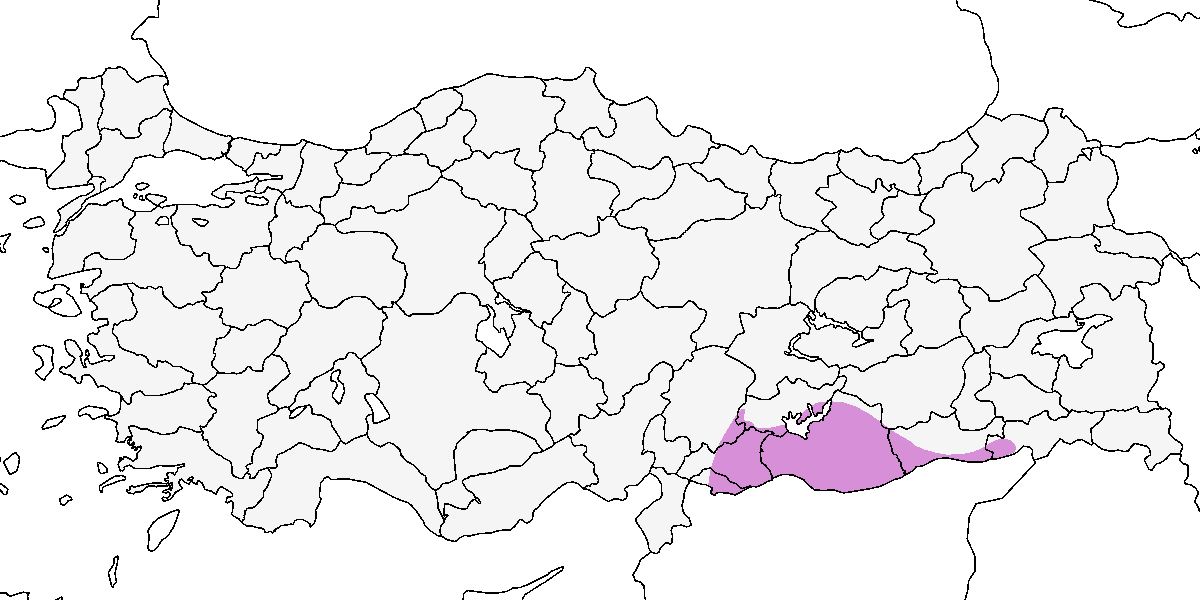
\includegraphics[keepaspectratio]{images/harita_Rhodospiza obsoleta.png}}

\textbf{Üreme}

\textbf{Yuvalama alanı:} Kurak bölgelerdeki zeytin ve fıstık
bahçelerinde, çalılık arazilerde ve çitlerde, sıkça tarla ve bahçelerin
yakınında ürer.\\
\textbf{Yuvası:} Yuvasını ağaç veya çalılara, yerden 1,3--3,0 m yükseğe,
yatay dalların ucuna veya çatallarına yapar. Yuva dallar, ot ve köklerle
örülür, beyaz renkli bitkisel lif, ince otlar, kıl ve yünle
astarlanır.\\
\textbf{Yumurta sayısı:} Türkiye'de iki yuvada üç yumurta, bir yuvada
dört yumurta, bir yuvada beş yumurta ve üç yuvada altı yumurta tespit
edilmiştir. Bir yuvada iki yavru ve iki yuvada beş yavru
kaydedilmiştir.\\
\textbf{Üreme dönemi:} Nisan ve mayıs ayında yumurta koyar. Yılda iki
kez kuluçkaya yattığı düşünülmektedir. \textbf{GDA:} Çoğu üreme kaydı
Gaziantep ve Birecik'tendir. 23 Nisan 1972'de dört yuvada üçer, altı ve
bir yumurta kaydedilmiş, tek yumurta bulunan yuvada kuluçkanın henüz
tamamlanmadığı anlaşılmıştır (McNeile, 1950, 1951, 1954, 1967, 1968,
1970, 1972, 1973). Mayıs ayında bir yuvada yumurtalar, diğer üç yuvada
ise 4 Mayıs 1964'te yavrular, 5 Mayıs 1970'te beş yavru, 16 Mayıs
1985'te iki yavru görülmüştür (Warncke, 1964-\/-65). 10--11 Mayıs
2004'te iki çiftin dişileri yuva malzemesi taşırken gözlenmiş, 23 Mayıs
2004'te bir bireyin bir ağaç fidesine yuva yaptığı kaydedilmiştir. 17
Mayıs 2004'te bulunan bir yuvada beş yumurta, ertesi günlerde altıncı
yumurta da gözlenmiştir. 7 Haziran 2006'da bulunan bir yuvada iki günlük
beş yavru sayılmıştır. İkinci kuluçkaya ait olduğu düşünülen kayıtlar
şunlardır: 4 Haziran 1993'te yuva yapımı, 5 Haziran 1993'te dört ve beş
yumurtalı iki yuva, 12 Haziran 2006'da altı yumurtalı bir yuva
kaydedilmiştir. 2 Temmuz 1978'de Akçakale'de tüylenmiş en az üç yavruyu
besleyen bir erkek ve 16 Ağustos 1974'te Güreniz yakınında iki aile
grubu gözlenmiştir. \textbf{DOA:} 5 Ağustos 1992'de Doğubayazıt'ta bir
aile grubu kaydedilmiştir.

\textbf{Alttürler ve Sınıflandırma}

Monotipik bir türdür. \emph{Rhodospiza} cinsi geçmişte sıklıkla
\emph{Rhodopechys} cinsinin bir alt grubu olarak değerlendirilmiştir.
Ancak birbirinden bağımsız çalışmalarla elde edilen güçlü genetik
veriler, bu türün ayrı bir cins olarak ele alınması gerektiğini
desteklemektedir (Groth, 1998; Arnaìz-Villena \emph{vd.}, 2008).
Taksonomiyle ilgili daha fazla bilgi için Doğu Alamecek'i hakkındaki
tartışmalara bakınız.

\section{Florya}\label{florya}

\emph{Chloris chloris}, European Greenfinch

\textbf{\emph{Yaygın olarak çok sayıda bulunan yerli, geçit türü ve kış
göçmenidir.}}

En çok sayıda Marmara, Ege, Akdeniz ve Karadeniz bölgelerinde görülür.
İç Anadolu'nun kenarlarında ve Güneydoğu Anadolu'nun batısında daha
lokal olarak bulunur. Marmara, Orta Toroslar ve Kuzeydoğu Anadolu
dağlarında 2000 metreye kadar olan ağaçlık habitatlarda ürer. Kısmen
göçücü veya irtifa göçmenidir.

Göç döneminde, özellikle sonbaharda daha yaygındır. Eylül sonundan kasım
başına kadar İstanbul Boğazı ve Akdeniz kıyılarında yüksek sayılarda
kaydedilir. Geçiş genellikle 25 Eylül'de başlar ve ekim ayının ikinci
yarısında yoğunlaşır. İlkbahar geçişi daha belirsizdir, mart ve nisan
aylarında gerçekleşir. Kış döneminde en çok Ege ve Akdeniz'de, ayrıca
Marmara, Karadeniz ve daha az sayıda olmak üzere İç Anadolu'da görülür.
Bu dönemde sıklıkla diğer ispinoz türleriyle karışık sürüler oluşturur.

\pandocbounded{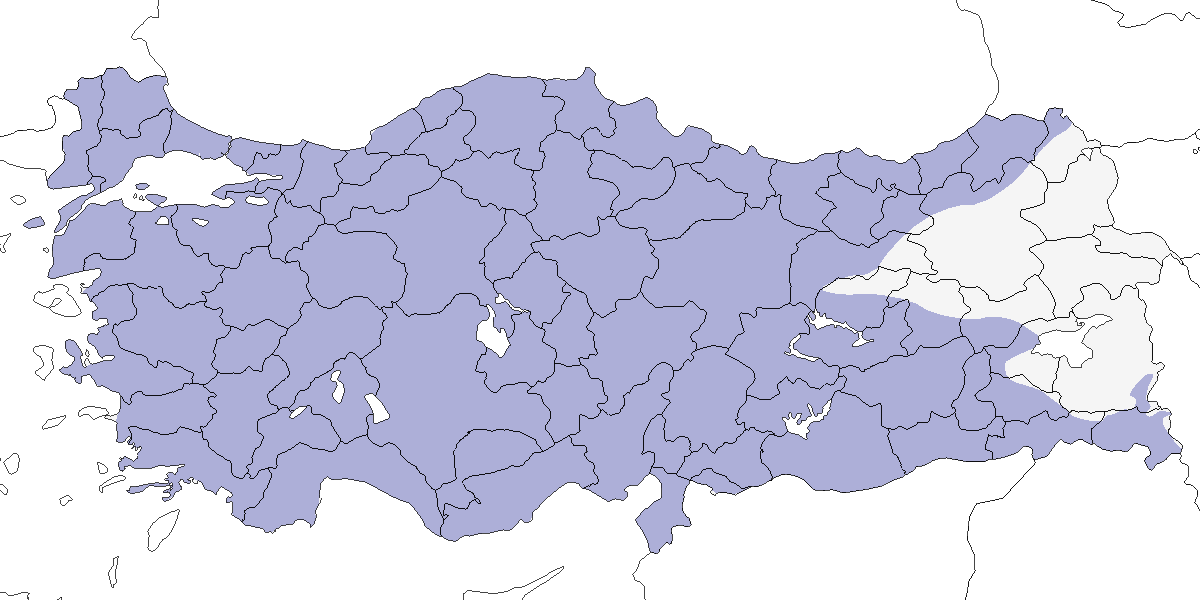
\includegraphics[keepaspectratio]{images/harita_Chloris chloris.png}}

\textbf{Üreme}

\textbf{Yuvalama alanı:} Ağaçlık ve çalılık açık arazilerde, özellikle
orman kenarlarında, meyve bahçelerinde, zeytinliklerde, parklarda,
bahçelerde ve ağaç sıralarında ürer.\\
\textbf{Yuvası:} Yuvasını bir çalıya veya ağaca yerden 2--4 m yüksekliğe
kurar.\\
\textbf{Yumurta sayısı:} Türkiye'de iki yuvada dört yumurta, bir yuvada
altı yumurta tespit edilmiştir.\\
\textbf{Üreme dönemi:} Nisan ortasından itibaren yumurta koyar. Gençler
ağustosa kadar görülür. Bu olgu, Türkiye'de de yılda iki kez kuluçkaya
yatıldığını göstermektedir. \textbf{MAR:} 25 Haziran 1973'te Eceabat
yakınında yiyecek taşıyan bir erişkin gözlenmiş, 26 Haziran 1973'te
Küçükkuyu'da görülen yeni tüylenmiş yavru, yumurtlamanın mayıs sonunda
gerçekleştiğini göstermiştir. \textbf{KAD.} 15 Haziran 1984'te
Kızılırmak Deltası'nda ve 8 Haziran 1986'da Yeniçağa Gölü'nde tüylenmiş
yavrular kaydedilmiştir (Kılıç \& Kasparek, 1987). \textbf{AKD:} 5 Mayıs
2003'te Dalaman'da bir sıra oluşturan çalımsı ibreli ağaçlarda biri
henüz kuluçkaya yatılmamış tek yumurtalı, biri üç yumurtalı, biri altı
yumurtalı ve biri de yumurtadan yeni çıkmış bir yavru içeren dört yuva
bulunmuştur; bu son yuva, yumurtlamanın yaklaşık 19 Nisan'da başladığını
göstermektedir. \textbf{EGE:} 23 Mayıs 1999'da Milet'te bir böğürtlen
çalısında dört yumurtalı bir yuva bulunmuştur. \textbf{İÇA:} 8 Nisan
1984'te Kızılcahamam'da yuva yapımı gözlenmiştir (Barış \emph{vd.},
1984). \textbf{DOA:} 24 Ağustos 1972'de Van Gölü yakınında bir genç
birey görülmüştür. \textbf{GDA:} 14 Haziran 1996'da Gaziantep Işıklı'da
gözlem yapılmıştır.

\textbf{Alttürler ve Sınıflandırma}

Türkiye genelinde floryaların büyük çoğunluğu Güney Avrupa kökenli
\emph{aurantiiventris} alttürüne aittir. Güneydoğu Anadolu ve çevresinde
ise \emph{chlorotica} alttürü bulunur. Floryanın bölgesel formlarını
sınıflandırma çabaları çoğunlukla sonuçsuz kalmıştır. Daha önce Marmara
ve Kuzey Ege'de \emph{muehlei}, Kuzeydoğu Anadolu'da \emph{bilkevitchi}
ve Hatay'da \emph{chlorotica} alttürlerinin bulunduğu öne sürülmüş,
ayrıca Güney Ege'den örnek bulunmamasına rağmen burada da
\emph{aurantiiventris} alttürünün varlığı önerilmiştir (Roselaar, 1995).
Ancak günümüzde \emph{muehlei} ve \emph{bilkevitchi} taksonları,
\emph{aurantiiventris} alttürünün sinonimi olarak kabul edilmektedir.

\section{Sarı Gagalı Ketenkuşu}\label{sarux131-gagalux131-ketenkuux15fu}

\emph{Linaria flavirostris}, Twite

\textbf{\emph{Lokal olarak az sayıda bulunan yerli ve irtifa
göçmenidir.}}

Doğu Karadeniz Bölgesi, Doğu Anadolu'nun hemen hemen her yerinde ve
Güneydoğu Anadolu'nun en doğusunda, genellikle yüksek irtifalarda çıplak
ve kayalık bölgelerde bulunur. Doğu Anadolu'nun güney kesimlerinde 1000
m rakıma kadar iner. Batıda İç Anadolu'nun doğu ve kuzey sınırlarında,
muhtemelen Akdeniz Bölgesi'ne kadar ulaşır. Genellikle 1750 ile 3000 m
arasında görülür, ancak Büyük Ağrı gibi yüksek dağlarda en az 4500 m'ye
kadar çıkar. Kar çizgisi çevresinde yuvalar ve üremeye mayıs ortasında
başlar. Üreme sonrasında 400 bireye kadar sürüler oluşturabilir.

Genellikle ekim ve nisan başı arasında kışı geçirmek üzere daha alçak
bölgelere iner. Kışın, Doğu Anadolu'da 2000 m'ye kadar olan
yüksekliklerde çoğunlukla 200 bireye kadar çıkan sürüler hâlinde yaygın
ve boldur. Bu dönemde batıya doğru biraz yayılır, 900 m'ye kadar iner ve
çok nadiren Ankara çevresinde görülür. Akdeniz Bölgesi'nde üreme dönemi
sonunda 1000 m'ye kadar iner.

\pandocbounded{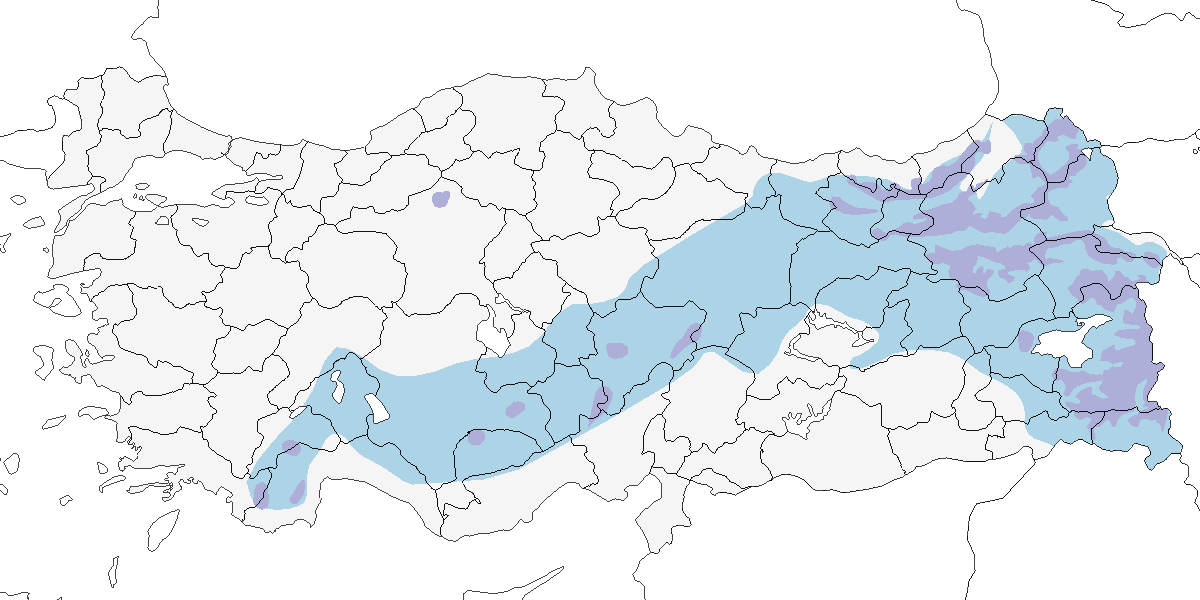
\includegraphics[keepaspectratio]{images/harita_Linaria flavirostris.png}}

\textbf{Üreme}

\textbf{Yuvalama alanı:} Ağaç çizgisinin üzerinde, cılız bitkilerle
kaplı çıplak ve kayalık yamaçlarda ürer.\\
\textbf{Yuvası:} Türkiye'den doğrudan yuva kaydı yoktur. Diğer
bölgelerde yerde, alçak bitki örtüsünün altında, toprak yamaçlardaki
deliklerde, kaya çıkıntılarının altlarında ve bazen çalılıkların içinde
yuva yapar. Kâse şeklindeki yuva ot ve bitki kökleriyle örülür, yün, kıl
ve tüylerle astarlanır.\\
\textbf{Yumurta sayısı:} Türkiye'de veri yoktur. Diğer bölgelerde olağan
yumurta sayısı 5--6'dır.\\
\textbf{Üreme dönemi:} Mayıs ayından itibaren yuva yapmaya ve yumurta
koymaya başlar. temmuzdan sonra yavrular yuvadan ayrılır. \textbf{KAD.}
13 Temmuz 1975'te İspir ile Rize arasında henüz yeni uçmaya başlamış bir
yavru gözlenmiş, yumurtlamanın haziran ortasında gerçekleştiği
düşünülmüştür. 14 Ağustos 1972'de Rize'de üç erişkin ve bir genç, 11
Ağustos 1966'da Bayburt çevresinde iki aile grubu görülmüştür.
\textbf{DOA:} 7 Mayıs 2004'te Erçek yakınında kısa otlarla kaplı, kaya
kütlelerinin bulunduğu dik bir yamaçta çiftleşen bir çift ve yuva yapan
bir dişi gözlenmiştir. Yuva, yerden 2 m yukarıda, alçak bir uçurumun dar
bir çıkıntısı üzerinde, yukarıdan sarkan bitkilerin gölgesindeydi. 5
Ağustos 1992'de Bendimahi'nin 45 km kuzeyindeki lav akıntısında bir aile
grubu görülmüştür. \textbf{İÇA:} 22 Mayıs 1972'de Ürgüp'ün doğusundaki
Tekke Dağı'nda bir çift üreme davranışı sergilemiş, 19 Ağustos 2004'te
Kızılcahamam'da tüylenmiş bir yavru kaydedilmiştir.

\textbf{Alttürler ve Sınıflandırma}

Türkiye, Kafkaslar, Kuzey Irak ve Kuzey İran'da \emph{brevirostris}
alttürü bulunur (Vaurie, 1959c; Roselaar, 1995). Bu alttürün üst ve alt
taraf zemini, nominat \emph{flavirostris} ve Britanya'daki
\emph{pipilans} alttürüne kıyasla belirgin şekilde daha açıktır
(Roselaar, 1995). Alt taraftaki çizgiler daha siliktir; özellikle
erkeklerde lekeler daha belirgin, düzenli ve kalındır (Kumerloeve,
1967c; Sharpe, 1888; Sushkin, 1925). Pembe kuyruk sokumu, Kuzeybatı
Avrupa alttürlerine göre daha canlı ve kırmızımsı tondadır.

\section{Ketenkuşu}\label{ketenkuux15fu}

\emph{Linaria cannabina}, Common Linnet

\textbf{\emph{Yaygın olarak çok sayıda bulunan yerli, geçiş türü ve kış
göçmenidir.}}

Genellikle 3000 m'ye kadar, bazı yerlerde 4200 m'ye kadar yüksekliğe
çıkar; ovalarda ise nadirdir. Üreme dönemi çoğunlukla nisan ayında
başlar. Güneydoğu Anadolu'daki yayılışı batı ve kuzeybatı kesimleriyle
sınırlıdır. Dağlık alanlarda muhtemelen irtifa göçü yapar.

Geçit sırasında çok daha yaygın ve boldur. İstanbul Boğazı'nda 11
Ağustos--20 Kasım arasında, Marmara kıyılarında ise daha geç tarihlerde
kaydedilir. Kışın Trakya, Batı ve Orta Anadolu'nun ovalarında ekim ile
mart ayları arasında düzenli olarak görülür ve zaman zaman 2000 bireye
ulaşan büyük sürüler oluşturur.

\pandocbounded{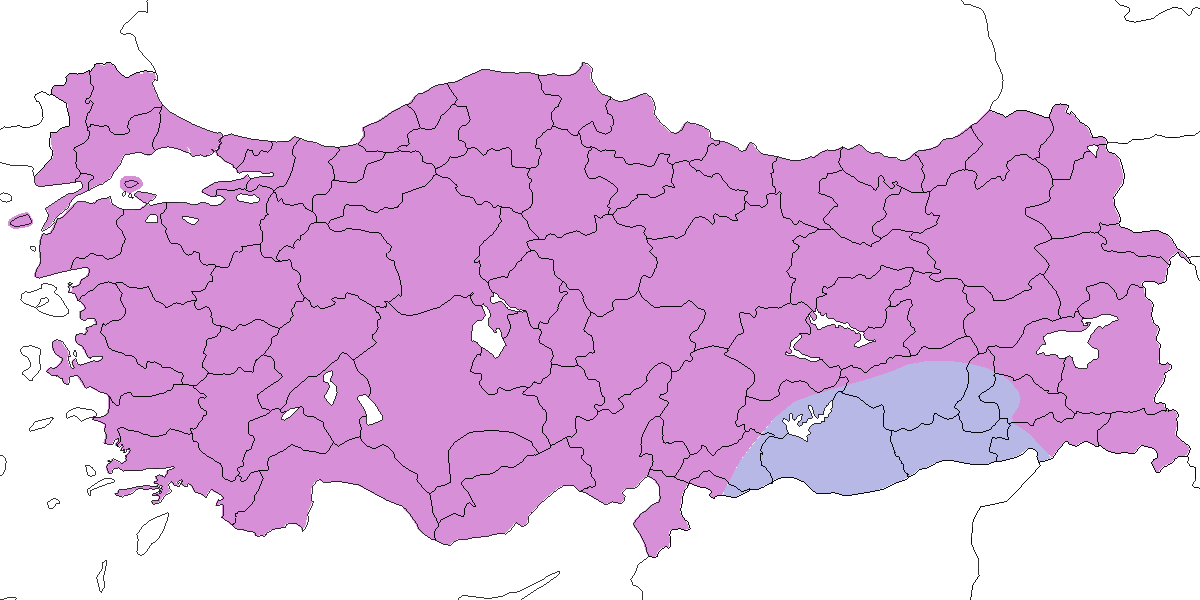
\includegraphics[keepaspectratio]{images/harita_Linaria cannabina.png}}

\textbf{Üreme}

\textbf{Yuvalama alanı:} Deniz seviyesinden alpin çayırlara kadar
değişen irtifalarda, çalılık alanlarda ürer.\\
\textbf{Yuvası:} Kâse şeklindeki yuvasını bir çalının içine ot, bitki
kökleri ve yosunlardan örer, kıl veya yünle astarlar.\\
\textbf{Yumurta sayısı:} Türkiye'de üç yumurta bulunan üç yuva, dört
yumurta bulunan beş yuva ve beş yumurta bulunan altı yuva tespit
edilmiştir.\\
\textbf{Üreme dönemi:} Nisan başından itibaren yumurta koyar. Mayıs
itibariyle yavrular gözükür. Yayılış gösterdiği diğer alanlarda olduğu
gibi Türkiye'de de yılda iki kez kuluçkaya yatar. \textbf{MAR:} 21
Temmuz 1993'te Uludağ'da bir erkek iki yavruyu beslerken görülmüş, 12
Mayıs 1964'te kuluçkası tamamlanmamış tek yumurtalı bir yuva bulunmuştur
(Warncke, 1964-\/-65). 25 Haziran 1973'te Alexandria Troas Antik Şehri
ve Çanakkale Kösedere'de yeni tüylenmiş yavrular kaydedilmiştir.
\textbf{AKD:} 28--29 Nisan 1970'te Aladağ'da yuva yapımı, 8 Mayıs
1970'te İslahiye'de beş yumurtalı bir yuva kaydedilmiştir. 30 Nisan
1967'de Akseki'de bir çift yuva malzemesi toplarken gözlenmiştir.
Haziran 1966'da Aladağ'da birçok genç, 5 Haziran 1985'te Acıgöl'de 5--6
genç kaydedilmiştir (Dijksen \& Kasparek, 1988). 13 Mayıs 2004'te
Demirkazık'ta bir yuvada beş yumurta, 10 ve 13 Mayıs 2005'te Mut'taki üç
yuvadan ikisinde dörder yumurta, birinde ise yavrular gözlenmiştir.
\textbf{KAD.} 3 Haziran 1945'te Abant Gölü'nde bir erkek bir yavruyla
birlikte gözlenmiştir (Wadley, 1951). \textbf{İÇA:} 28 Nisan 1972'de
yeni ve boş bir yuva görülmüş, 13 Nisan 1970'te uzun süredir kuluçkada
olan dört yumurtalı bir yuvanın yumurtlama tarihinin mart sonu veya
nisan başı olduğu anlaşılmıştır (McNeile, 1950, 1951, 1954, 1967, 1968,
1970, 1972, 1973). 6 Mayıs 1993'te Kızılcahamam'da bir yuvada üç
yumurta, 14 Haziran 1993'te dört yumurta, 27 Mayıs 1993'te Hasan Dağ'da
üç yumurtalı bir yuva kaydedilmiştir. 20 Nisan 2004'te Karapınar
yakınlarında iki günlük dört yavru bulunan bir yuvada yumurtlama
tarihinin 3 Nisan olduğu hesaplanmıştır. 18 Haziran 1998'de Aksaray'da
erişkinlerin tüylenmiş yavruları beslediği görülmüştür. \textbf{GDA:} 16
Haziran 2001'de Yeşilce'deki bir yuvada üç yumurta, 20 Mayıs'ta diğer
bir yuvada bir yumurta ve dört yeni çıkmış yavru tespit edilmiştir. 2
Mayıs 1964'te Gaziantep'te dört küçük yavru içeren bir yuvanın
yumurtlama tarihi nisan ortası olarak tahmin edilmiştir (Warncke,
1964-\/-65). 15 Haziran 1996'da Işıklı'da birçok tüylenmiş yavru
gözlenmiştir. 1 Mayıs 1970'te Osmaniye yakınlarındaki bir yuvada beş
yumurta sayılmış, 9 Mayıs 2004'te Durnalık'taki iki yuvada dört ve beş
yumurta tespit edilmiştir.

\textbf{Alttürler ve Sınıflandırma}

Üreme döneminde incelenen tüm örneklerin \emph{bella} alttürüne ait
olduğu düşünülmektedir (Roselaar, 1995). Ancak kış döneminde, örneğin
Erzurum'da \emph{cannabina} alttürüne ait bireyler de kaydedilmiştir.
Trakya'da toplanmış örnek bulunmamakla birlikte, burada üreyen
bireylerin \emph{cannabina} ya da \emph{cannabina} ile \emph{bella}
arasındaki geçiş formuna ait olabileceği öne sürülmüştür (Roselaar,
1995).

Bu alttürün morfolojik varyasyonları ayrıntılı olarak incelenmiştir
(Vaurie, 1949). \emph{Bella}, \emph{cannabina}'dan daha iri yapılı ve
açık renkli olup, kuyruk sokumu ve kuyruk üstü örtüleri neredeyse
çizgisizdir; alnındaki pembemsi kırmızı alan ise daha soluk ve dardır.

Ketenkuşu ve Sarı Gagalı Ketenkuşu geçmişte \emph{Acanthis} cinsi
altında sınıflandırılmıştır (Marten \& Johnson, 1986; Elzen \&
Nemeschkal, 1991; Fehrer, 1996; Arnaìz-Villena \emph{vd.}, 2001). Bazı
kaynaklarda ise \emph{Carduelis} cinsine dahil edilmiştir.

\section{Huş İsketesi}\label{huux15f-isketesi}

\emph{Acanthis flammea}, Common Redpoll

\textbf{\emph{Rastlantısal konuktur.}}

5 Ocak 1987'de Burdur Gölü'nde yaklaşık 10 bireyden oluşan bir sürü
(Magnin, 1989), 26 Mart 1992'de (yayında 25 Mart olarak hatalı
verilmiştir) Kızılırmak Deltası'nda kuzeye göç eden 25 birey (Kirwan,
1992) ve 15 Kasım 2005'te Ankara Altınpark'ta E. Yoğurtçuoğlu tarafından
fotoğraflanan bir birey.

İstanbul ve İstanbul Boğazı'ndan çeşitli tarihî kayıtlar da mevcuttur.
Robson, bu bölgede kışın türü yüksek sayılarda kaydettiğini bildirmiş,
ancak tarih vermemiştir (Krüper, 1875). 1890--91 kışında Üsküdar'da bir
sürü gözlenmiş, Alléon 20 ve 30 Ocak 1899'da Büyükdere ve Makriköy'de
birer birey toplamış ve bu örnekler bugün Sofya Doğa Tarihi Müzesi'nde
korunmaktadır (Mathey-Dupraz, 1920--24). Türün İstanbul'da bulunduğu
bilinmektedir (Braun, 1903) ve bu veriler, 1902--03 kışında küçük çaplı
bir akın olduğunu düşündürmüştür (Kasparek, 1990). Ayrıca, 3 Şubat
1947'de Zonguldak Çatalağzı'nda gözlenmiş (Ogilvie, 1954) ve Ekim ile
Kasım 1941'de komşu Bulgaristan'da iki kez kaydedilmiştir (Kumerloeve,
1957).

\pandocbounded{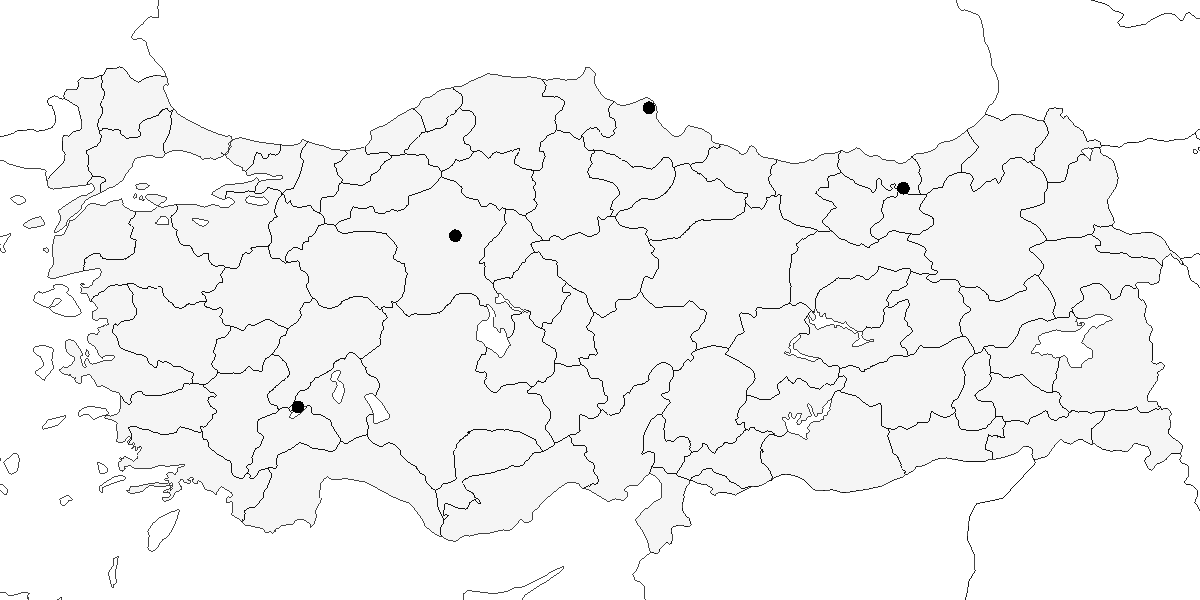
\includegraphics[keepaspectratio]{images/harita_Acanthis flammea.png}}

\textbf{Üreme}

Türkiye'de yuvalamaz. Üreme dönemi yayılış alanı Kuzey Avrupa, Asya ve
Amerika'dır.

\textbf{Alttürler ve Sınıflandırma}

Türkiye'den gelen tüm kayıtların \emph{nominat flammea} alttürüne ait
olduğu kabul edilebilir. Alléon tarafından toplanan iki örnek bu alttüre
aittir ve günümüzde Robert Kolej koleksiyonunda bulunmayan örneğin de
\emph{flammea} olduğu belirtilmiştir (Mathey-Dupraz, 1920--24).
\emph{Flammea}, İskandinavya'dan doğuda Kamçatka'ya ve ötesinde Alaska
ile Kuzey Kanada'ya kadar uzanan geniş bir üreme alanına sahiptir
(Clement \emph{vd.}, 1993).

\section{Çaprazgaga}\label{uxe7aprazgaga}

\emph{Loxia curvirostra}, Red Crossbill

\textbf{\emph{Nispeten lokal olarak az sayıda bulunan yerlidir.}}

Saf ve karışık ibreli ormanlarda çok yerel olarak, ancak genellikle az
sayıda bulunur. Karadeniz Bölgesi'nde özellikle doğu kesimlerinde
yoğunlaşırken, batıya doğru daha seyrekleşir. Güney Marmara'da en çok
Uludağ'da görülür, diğer alanlarda düzensizdir. İç Anadolu'nun kuzey
sınırında, özellikle Ankara Beynam Ormanı'nda lokal bir popülasyon
varlığını sürdürür. Akdeniz Bölgesi'nde ise Toroslar boyunca yayılış
gösterir. Üreme dönemi boyunca 2500 m'ye kadar çıkabilse de, genellikle
daha düşük rakımlarda, örneğin Toroslar'da 800--900 m civarında bulunur.

Sonbahar ve kış aylarında, özellikle yurtdışından gelen bireylerin de
katıldığı muhtemel akın yıllarında daha yaygın hâle gelir. Diğer
bölgelerde ilkbahar gözlemleri ise büyük olasılıkla geçit yapan
bireylere aittir.

\pandocbounded{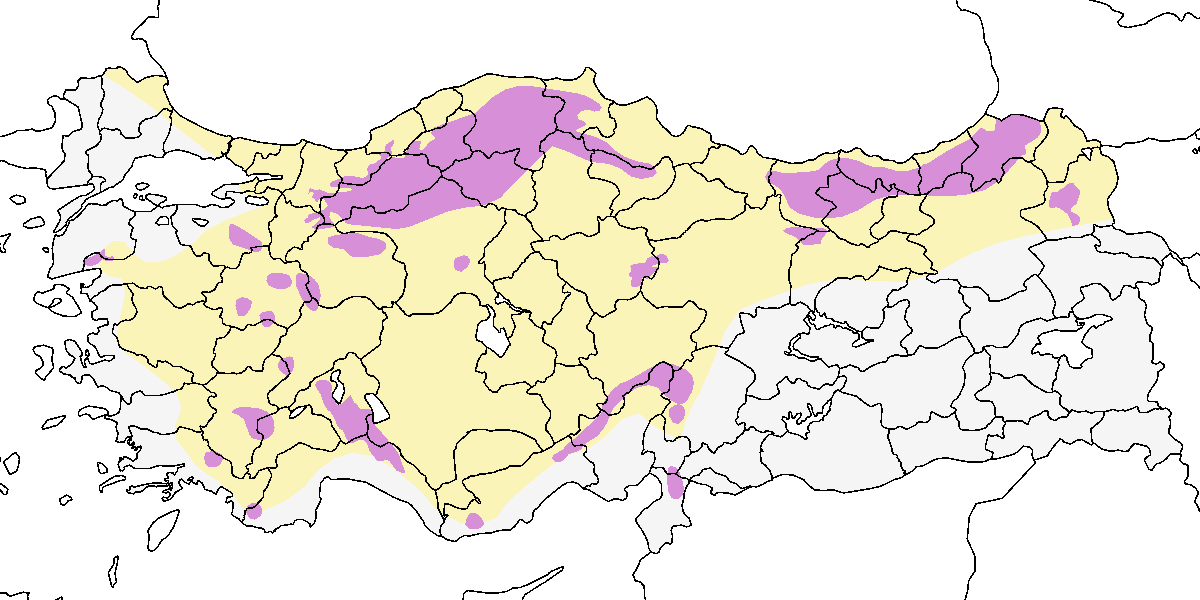
\includegraphics[keepaspectratio]{images/harita_Loxia curvirostra.png}}

\textbf{Üreme}

\textbf{Yuvalama alanı:} Dağlık çam ormanlarında ürer. Türkiye'de
yalnızca tüylenmiş yavrular ve gençler gözlenmiştir.\\
\textbf{Yuvası:} Başka bölgelerde yuvasını özellikle oldukça seyrek
ibreli ormanlarda, yerden 2--18 m yükseklikte, çoğunlukla 8 m'den
yukarıda ve ağaçların dış dallarına yapar. Yuva temeli dallardan oluşur,
üst kısmı yosun ve likenlerle örülür; içi ince otlar, kıllar ve tüylerle
kaplanır.\\
\textbf{Yumurta sayısı:} Türkiye'den veri yoktur. Diğer bölgelerde
olağan yumurta sayısı 3--4 olup, nadiren 2 ya da 5 olabilir.\\
\textbf{Üreme dönemi:} Üreme mart ayında başlar. Kayıtlar yumurtlamanın
nisan ayının ilk yarısında gerçekleştiğini gösterir. Besin bol olduğu
yıllarda yılda iki kez kuluçkaya yattığı bilinmektedir. \textbf{MAR:} 21
Mayıs 1970'te Keşan'da yiyecek taşıyan bir erişkin kaydedilmiştir.
\textbf{AKD:} 19 Mayıs 1984'te Akseki yakınında bir dişinin iki
tüylenmiş yavruyu beslediği, 28 Mayıs 1996'da ise yeni tüylenmiş bir
genç görüldüğü kaydedilmiştir. Bu ikinci gözlemdeki birey henüz yeni
tüylenmişse yumurtlama tarihi 12--21 Nisan arasında olmalıdır.
\textbf{KAD.} Haziran ve ağustos ayları arasında genç bireyler
gözlenmiştir. İç Anadolu'da ağustosta görülen gençlerin birkaç ay önce
tüylendikleri, yani daha olgun bireyler oldukları düşünülmektedir.
\textbf{İÇA:} 9 Mayıs 1990'da Daday'da bir dişi ve üç genç, 29 Mayıs
1992'de Kızılcahamam yakınında ibreli ormanda bir erişkin ile yeni
tüylenmiş gençler gözlenmiştir.

\textbf{Alttürler ve Sınıflandırma}

Türkiye'deki tüm popülasyonların \emph{guillemardi} alttürüne ait olduğu
kabul edilmektedir. Batı Karadeniz'deki bireyler daha önce
\emph{vasvarii}, Kafkas Dağları ve Güney Kafkasya'daki bireyler ise
\emph{caucasica} olarak tanımlanmıştır (Roselaar, 1995). Bu iki takson
Kıbrıs'ta tanımlanan \emph{guillemardi} alttürünün sinonimi olarak
değerlendirilmelidir.

\section{Saka}\label{saka}

\emph{Carduelis carduelis}, European Goldfinch

\textbf{\emph{Yaygın olarak çok sayıda bulunan bulunan yerli ve kış
göçmenidir.}}

Marmara, Ege ve Akdeniz bölgelerinde yaygın olarak ve çok sayıda, Doğu
ve Güneydoğu Anadolu'da lokal olarak bulunur. Doğu Anadolu'da çoğunlukla
göçmendir. Genellikle 1500 m'nin altındaki tarımsal alanlarda yaygındır,
ancak 2300 m'ye kadar da çıkabilir.

Geçit dönemlerinde oldukça yaygın olup zaman zaman büyük sayılarla
görülür. Sonbahar geçişi 14 Ağustos'tan itibaren başlar, çoğunlukla
ekimin ikinci yarısında yoğunlaşır ve kasım başına kadar sürer. Bu
dönemde floryalarla birlikte 12.000 bireyden oluşan karışık bir sürü
kaydedilmiştir. İlkbahar geçişi şubat sonu ile nisan başı arasındadır,
ancak bu dönemde belirgin bir yoğunluk dönemi gözlenmez. Kışın özellikle
Trakya, Batı ve Orta Anadolu'da sıkça görülür; bu dönemde 500 bireyi
aşan kalabalık sürüler oluşturur ve genellikle İspinoz, Florya,
Ketenkuşu ve bazen Büyük Baştankara ile karışık gruplar hâlinde dolaşır.

\pandocbounded{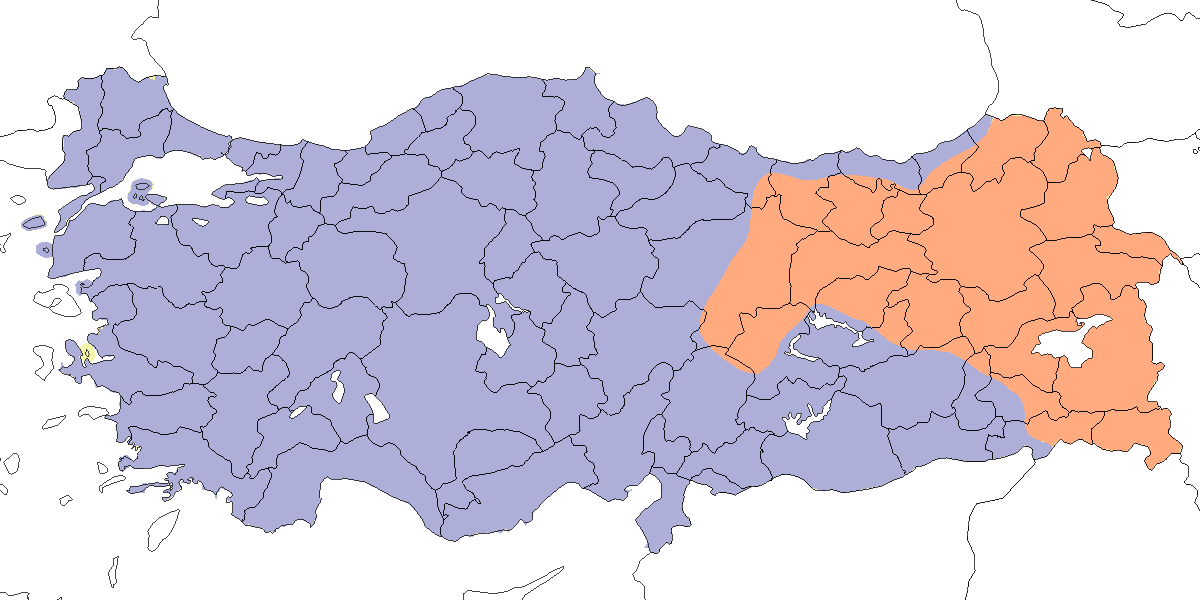
\includegraphics[keepaspectratio]{images/harita_Carduelis carduelis.png}}

\textbf{Üreme}

\textbf{Yuvalama alanı:} Özellikle tarımsal alanlar, meyve bahçeleri,
bahçeler, zeytinlikler ve narenciye bahçelerinde, ayrıca orman
kenarları, ılgınlar ve çalılık arazilerde yuvalar.\\
\textbf{Yuvası:} Yuvasını yüksek bir çalıya veya ağaca yapar. Otlar ve
köklerden muntazam bir kâse örer, yuva içini bitkisel havlar, kıl ve
yünle astarlar.\\
\textbf{Yumurta sayısı:} Türkiye'de dört yumurta bulunan beş yuva ve beş
yumurta bulunan iki yuva kaydedilmiştir. \textbf{Üreme dönemi:}
Çoğunlukla nisan ve mayıs ayında yumurta koymaya başlar. Hazirandan
itibaren tüylenmiş yavrular görülür. Haziran ayında görülen kayıtlar,
muhtemelen ikinci kuluçkaya aittir. \textbf{MAR:} 26 Haziran 1973'te
Gülpınar'da gözlenen yeni tüylenmiş yavrular, yumurtlamanın mayıs
sonunda gerçekleştiğini göstermektedir. \textbf{EGE:} 12--22 Mayıs
tarihleri arasında yumurtalı toplam yedi yuva kaydı vardır.
\textbf{AKD:} 1987'de Çukurova'da nisan ve mayıs aylarında yuvalar
kaydedilmiş (Have \& Berk, 1988), 18 Mayıs 1992'de Köyceğiz'de ve 24
Mayıs 1999'da Belek'te tüylenmiş yavrular görülmüştür. 22 Mayıs 2004'te
Göksu Deltası'nda bir dişi, ibreli bir ağaca yerden 7 m yükseğe yuva
yaparken gözlenmiş, başka bir ibreli ağaçta yerden 3 m yükseklikteki
yuvada beş yumurta bulunmuş, yine 22 Mayıs'ta yeni tüylenmiş yavrular
kaydedilmiştir. 12--13 Mayıs 2004'te Demirkazık'ta biri bir, diğeri iki
yumurtalı ve henüz kuluçkaya yatılmamış iki yuva ile yumurtasız hazır
yuvalar bulunmuştur. \textbf{KAD.} 6 Mayıs 1978'de Yeniçağa Gölü'nde
yuva yapımı kaydedilmiştir (Kılıç \& Kasparek, 1987). \textbf{İÇA:} Mart
başında sürüler dağılır, nisan başında çiftler belirir ve ötüşler
duyulur (Wadley, 1951). Mayıs başında yumurtalı yuvalar görülmüş
(Warncke, 1964-\/-65), 8 Haziran 1907'de yeni yapılmış bir yuva
bulunmuş, 10 Haziran'da uzun süredir kuluçkada olan yumurtalı bir yuva
ve 29 Haziran'da tüylenmiş yavrularla birlikte bir çift gözlenmiştir
(Ramsay, 1914). \textbf{GDA:} 10 Mayıs 2004'te Birecik'te neredeyse
tamamlanmış bir yuva bulunmuş, 23 Mayıs'ta dişi kuluçkaya yatmıştır. 14
Haziran 1996'da Işıklı'da tüylenmiş yavrular görülmüştür.

\textbf{Alttürler ve Sınıflandırma}

Trakya'daki popülasyonlar \emph{balcanica}, Orta ve Batı Anadolu'dakiler
\emph{niediecki} ve doğudakiler ise muhtemelen \emph{loudoni} alttürü
altında sınıflandırılır (Roselaar, 1995). \emph{Niediecki} alttürü
sakacılar arasında ``kömürcü saka'', \emph{balcanica} ise ``kasım
sakası'' olarak bilinir. Saka yetiştiricileri bu iki formu ötüşleri ve
davranışlarıyla ayırt edebilir.

Kara başlı alttürler arasında görülen varyasyonlar çoğunlukla klinaldir.
\emph{Loudoni} belirgin sınırları olan bir alttür değildir; Anadolu'da
batıdan doğuya doğru gidildikçe (yani \emph{niediecki}'den
\emph{loudoni}'ye doğru) tüylerdeki kahverengi miktarı artar. Roselaar,
bu geçiş zonunun kuzeyde Orta Karadeniz ile güneyde Fırat ve Dicle
havzalarını kapsayan bölgesine bir alttür atayamamıştır. Ayrıca
örneklerin tüy yıpranması ve solma durumu da sınıflandırmayı oldukça
zorlaştırmaktadır.

\emph{Balcanica} daha göçmen yapılıdır ve Balkanlar'dan soğuk havalarda
güneye iner. Çok sert kışlarda Karadeniz üzerinden Orta Asya kökenli
\emph{major} veya diğer kuzey alttürlerinin Doğu Karadeniz ve Doğu
Anadolu'ya kadar indiği düşünülür.

(Not: Saka taksonomisi Özgün Sözüer tarafından revize edilmiştir.)

\section{Küçük İskete}\label{kuxfcuxe7uxfck-iskete}

\emph{Serinus serinus}, European Serin

\textbf{\emph{Genellikle yaygın olarak çok sayıda bulunan yerlidir.}}

Dağlık bölgelerde yarı göçmen veya irtifa göçmenidir. Ege Bölgesi'nin
büyük kısmında, Marmara, Akdeniz ve Karadeniz Bölgeleri'nin tamamında
bulunur. İç Anadolu'nun kuzey, batı ve güney sınırlarında lokal olarak,
Güneydoğu Anadolu'nun batı kesimlerinde ise son derece sınırlı bir
yayılış gösterir. Genellikle 2000 metreye kadar olan ibreli ve karışık
ormanlarda, açık ormanlık alanlarda ve yüksek çalılıklarda ürer.

Geçit sırasında, sonbaharda ağustos ortasından ekim başına kadar,
ilkbaharda ise mart başından nisan sonuna kadar daha yaygın olarak
gözlenir. En geç 25 Nisan'da kaydedilmiştir. Kış aylarında Trakya, Batı
ve Orta Anadolu'da düzenli olarak görülür ve Güneydoğu Anadolu'nun
batısına kadar yayılır. Kasım ile nisan ayları arasında Birecik'ten de
kış kayıtları vardır. Bu dönemde Karadeniz kıyıları dâhil olmak üzere
kıyı bölgelerinde sık ve bazen 500 bireye ulaşan sürüler halinde
gözlenebilir.

\pandocbounded{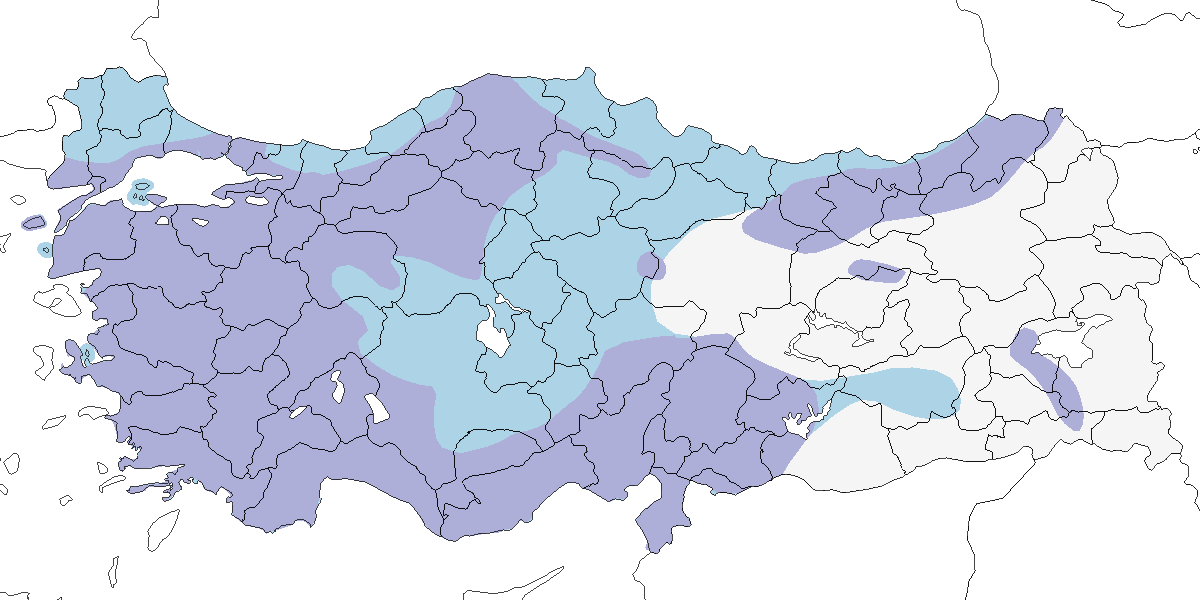
\includegraphics[keepaspectratio]{images/harita_Serinus serinus.png}}

\textbf{Üreme}

\textbf{Yuvalama alanı:} Açık ormanlar, meyve bahçeleri, parklar, ağaç
ve çitlerle çevrili tarlalar ve çalılıklarda bulunur.\\
\textbf{Yuvası:} Yuvasını bir ağaç veya çalıya yapar. Muntazam bir kâse
şeklindeki yuvasını bitki kökleri, otlar ve yosunlarla örer, içini kıl
ve bitkisel havla astarlar.\\
\textbf{Yumurta sayısı:} Türkiye'de beş yumurta içeren bir yuva
kaydedilmiştir. Yavru sayısı hakkında bilgi yoktur.\\
\textbf{Üreme dönemi:} Yumurtlama mart sonu ile mayıs ayı arasında
gerçekleşir. \textbf{EGE:} 28 Haziran 1984'te Ayvalık'ta iki erişkinle
birlikte 2--3 genç gözlenmiştir. \textbf{MAR:} Temmuz 1966'da Küçük
Çamlıca'da tüylenmiş yavrular ve 21 Temmuz'da yuva yapımı kaydedilmiş,
bu kayıtlar türün iki kez kuluçkaya yattığını göstermektedir.
\textbf{AKD:} 20 Mart 1987'de Çukurova'da 12 öten erkek gözlenmiş,
12--14 Mayıs 1987 arasında birçok yuva yeri tespit edilmiştir (Have \&
Berk, 1988). 19 Nisan 2004'te Akseki'de bir köknarda yerden 2,2 m
yüksekte örülmüş ancak henüz astarlanmamış bir yuva bulunmuştur. 7 Mayıs
2003'te Söğüt yakınında seyrek çalılıklı bir yamaçta, sık bir ardıcın
içinde yerden 1,6 m yüksekte beş yumurtalı bir yuva kaydedilmiştir. 30
Nisan 1989'da Ağla'da, 5 Mayıs 1996'da Dalyan'da, 23 Mayıs 1970'te Niğde
çevresinde ve 5 Haziran 1999'da Bolkar Dağları'nda gözlenen tüylenmiş
yavrular görülmüştür.

\textbf{Alttürler ve Sınıflandırma}

Monotipik bir türdür.

\section{Kara İskete}\label{kara-iskete}

\emph{Serinus pusillus}, Red-fronted Serin

\textbf{\emph{Nispeten lokal olarak çok sayıda bulunan yerli ve irtifa
göçmenidir.}}

Genellikle 1700--2800 metre arasında, alçak çalılıklarda ve bazen seyrek
ağaçlı kayalık yamaçlarda yaygın olarak bulunan yerli türdür. Yazın
nadiren 1000 metreye kadar iner; 3600 metreye kadar çıktığı
kaydedilmiştir. Batıdaki en uç yayılış noktası Batı Toroslar'daki Söğüt
Dağı'dır. Karadeniz Bölgesi'nin doğusunda, İç Anadolu'nun kuzey
sınırında, Güneydoğu Anadolu'nun tamamında ve Doğu Anadolu'da yaygındır;
ancak Doğu Anadolu'da bazı bölgelerde daha seyrektir. Bölgeden yalnızca
kuzeybatı uç kesimlerden ve Diyarbakır çevresinden kayıtlar vardır.
Marmara Bölgesi'nde Uludağ'da izole bir popülasyon yaşar; bunun yakın
zamanda gerçekleşmiş bir kolonizasyon olduğu öne sürülmüştür (Jetz,
1995). Ayrıca Ilgaz Dağları'nda uygun üreme habitatlarında yaz
döneminden en az iki kayıt mevcuttur. Üreme nisan ayında başlar, eylül
ayında sürü oluşturulmaya başlanır.

Sonbahar ve kış aylarında (ekim sonundan mart ortasına, istisnai olarak
nisan başına kadar), daha alçak rakımlara, hatta Akdeniz kıyılarına
kadar iner. Bu dönemde İstanbul Boğazı, Bodrum ve İzmir çevresinde
istisnai olarak kaydedilmiştir. Orta Karadeniz'de ise haziran başına
kadar deniz seviyesinde gözlenmiştir (Hustings \& Dijk, 1994). Kışın İç
Anadolu bozkırlarında daha yaygındır; ancak bu bölgede lokal yayılış
gösterir ve örneğin Ankara çevresinde oldukça nadirdir.

\pandocbounded{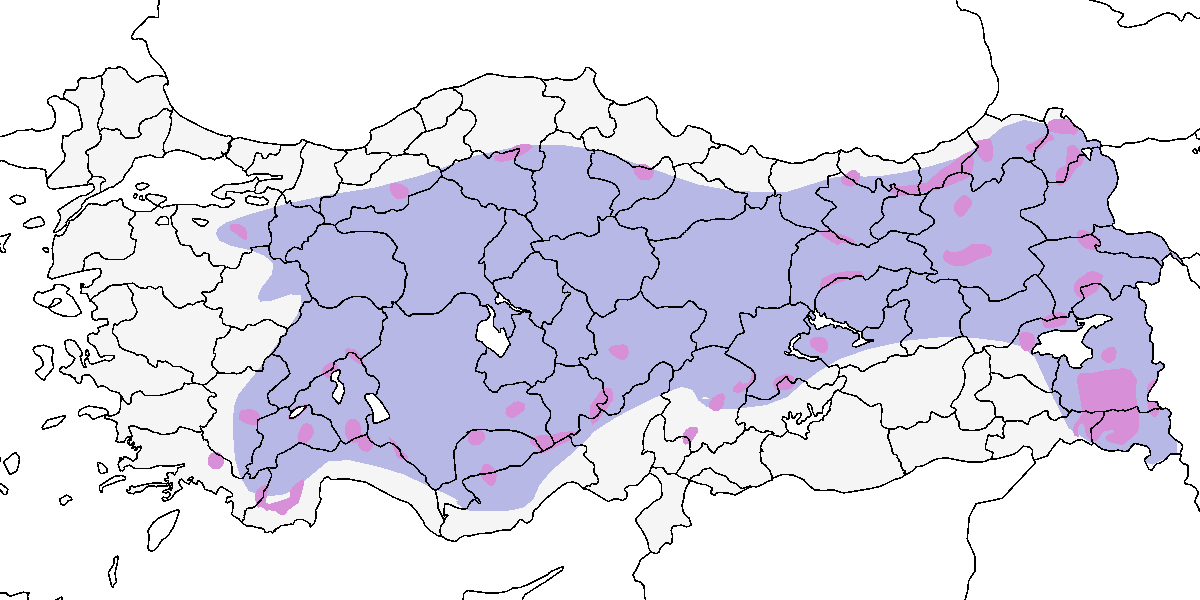
\includegraphics[keepaspectratio]{images/harita_Serinus pusillus.png}}

\textbf{Üreme}

\textbf{Yuvalama alanı:} Yüksek dağlık alanlarda, alçak çalılı kayalık
yamaçlarda bulunur. Çoğu yüksek dağda alpin kuşağın altında, genellikle
1800--3000 m arasında lokal olarak boldur. Alpin çayırlar, seyrek
ormanlar, çalılıklar ve özellikle bodur ardıçların bulunduğu karışık
habitatlarda yaşar (Green \& Moorhouse, 1995).\\
\textbf{Yuvası:} Sık bir çalının veya ardıcın içine, bazen ibreli bir
ağacın yüksek noktasına ya da kayaların arasındaki bir yarık ya da oyuğa
yapılır. Yuva derli toplu bir kâse şeklindedir; otlar, ağaç kabuğu
lifleri, bitki sapları ve yosunlarla örülür, içi bitkisel hav, kıllar,
yün ve tüylerle astarlanır.\\
\textbf{Yumurta sayısı:} Türkiye'de 21 Nisan 1876'da Aladağ'da bir
ardıcın yüksek noktasından alınan yuvada dört yumurta kaydedilmiştir.
Genellikle yumurta sayısı 3--5'tir.\\
\textbf{Üreme dönemi:} Haziran ayında yumurta koyar, temmuzdan eylüle
kadar tüylenmiş yavrular gözükebilir. Diğer bölgelerde yılda iki kez
kuluçkaya yatar. \textbf{MAR:} 1993'te Uludağ'da ağaç sınırı ve alpin
çalılıklarda yaygın olarak ürer. Temmuz itibariyle sürüler oluşturur
(Jetz, 1995); 25 Temmuz 1967'de bir erkekle birlikte birçok dişi veya
genç, 11 Eylül 1990'da iki erişkin ve bir genç ve 3 Haziran 2002'de
ağaçta öten bir erişkin kaydedilmiştir. \textbf{AKD:} 2 Temmuz--16
Ağustos 1966'da Karanfil Dağı'nda özellikle Berberis ve ardıç bulunan
vadilerde en bol tür olmuştur. 14 Temmuz'da bir erkek kur uçuşunda
gözlenmiş, 12 Ağustos'ta zirvede 10 genç birey tespit edilmiştir (Sutton
\& Gray, 1972). 9 Mayıs 1951'de Karanfil Dağı'nda 2150--2300 m arasında
ardıçlı alanlarda öten ve kurlaşan küçük sürüler kaydedilmiştir (Hollom,
1955). 28 Nisan 1973'te Akseki'de yuva yapan bir çift ve 11 Nisan
1973'te Elmalı'da sekiz erişkinden oluşan bir sürü, 25 Ağustos 1986'da
Demirkazık'ta dokuz erişkin ve dört gençten oluşan bir sürü
gözlenmiştir. \textbf{KAD.} 1 Eylül 1973'te Yalnızçam Geçidi'nde 2600 m
yüksekte iki tüylenmiş yavruyu besleyen bir çift ve 16 Haziran 1975'te
Trabzon Maçka'da öten bir erkek gözlenmiştir. \textbf{DOA:} 1 Haziran
1969'da Görentaş yakınlarında ardıç kalıntılarının bulunduğu kayalık
vadide on bireyden oluşan bir sürü, 5 Haziran 2001'de Nemrut Dağı'nda
dişisi yuva malzemesi taşıyan bir çift gözlenmiştir. \textbf{GDA:} 26
Temmuz 1972'de Gölbaşı Erkenek'te bir vadide üç genç birey gözlenmiştir.

\textbf{Alttürler ve Sınıflandırma}

Monotipik bir türdür.

\section{Kara Başlı İskete}\label{kara-baux15flux131-iskete}

\emph{Spinus spinus}, Eurasian Siskin

\textbf{\emph{Nispeten lokal olarak az sayıda ürer. Yaygın olarak çok
sayıda bulunan kış göçmeni ve geçit türüdür.}}

Marmara, Karadeniz, Ege, Akdeniz ve İç Anadolu'ya yakın bölgelerde,
800--2500 m arasındaki ibreli ve zaman zaman karışık dağ ormanlarında
küçük sayılarda yuvalar. Son yıllarda yaz aylarında Batı Toroslar'da,
özellikle Akseki civarında gözlenmiştir.

Eylül sonundan nisan başına kadar yaygın olarak çok sayıdadır. Özellikle
batı ve güney bölgelerinde ve alçak kesimlerinde kışlar. Doğu
Anadolu'nun batı kesimlerine de ulaşır. Güneydoğu Anadolu'dan Birecik,
Diyarbakır ve Halfeti'de az sayıda gözlenir. Sonbaharda İstanbul
Boğazı'nda eylül sonu ile kasım başı arasında, özellikle ekimin ikinci
ve üçüncü haftasında oldukça boldur. Örneğin, 1966'da Küçük Çamlıca'dan
toplam 2810 bireyin geçişi kaydedilmiştir. Bazı yıllarda geçit kasım
sonuna kadar devam eder. İlkbaharda ise göç en azından nisan sonuna
kadar sürer. Haziran başında Kızılırmak Deltası'ndan gelen bir gözlem
oldukça sıra dışıdır.

\pandocbounded{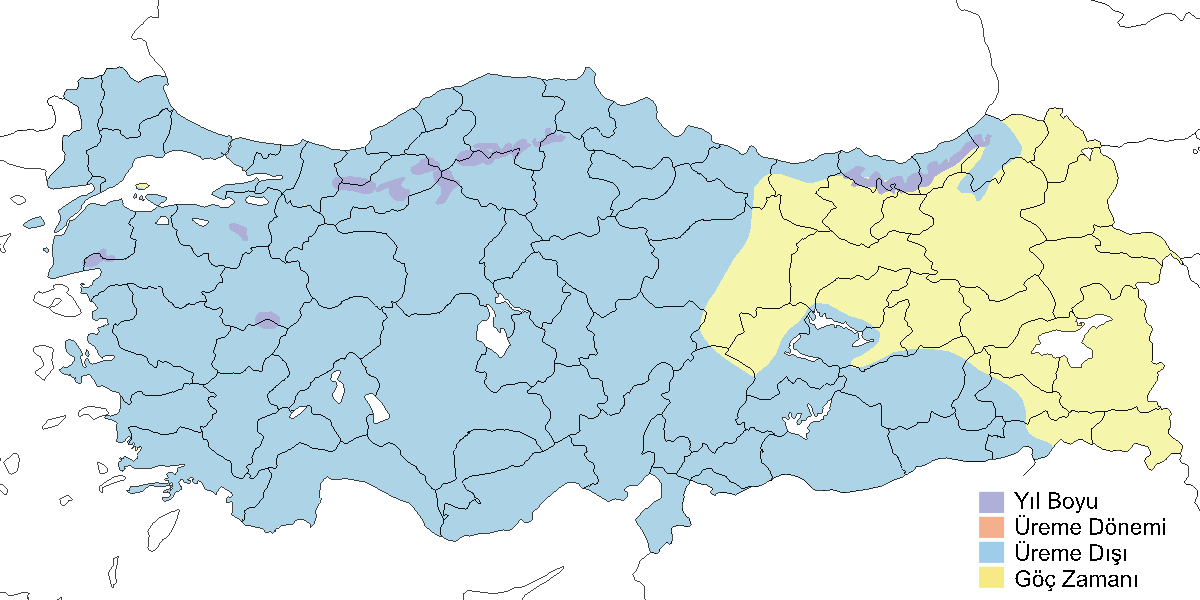
\includegraphics[keepaspectratio]{images/harita_Spinus spinus.png}}

\textbf{Üreme}

\textbf{Yuvalama alanı:} Dağlık ibreli ve karışık ormanlarda ürer.\\
\textbf{Yuvası:} İbreli ağaçlarda, genellikle yerden yüksekte bulunan
yuvası muntazam bir kâse şeklindedir; dallar, ot ve yosunlarla örülür,
içi kıl ve köklerle astarlanır.\\
\textbf{Yumurta sayısı:} Genellikle 4--5 yumurta bırakır.\\
\textbf{Üreme dönemi:} Türkiye'de mayıs ile haziran ayları arasında
ürer. Tür, yılda iki kez kuluçkaya yatar. \textbf{KAD.} Haziran başında
Abant Gölü'nde sıkça kur davranışı gösteren ve öten bireyler
kaydedilmiştir (Wadley, 1951). \textbf{EGE:} 9 Haziran 2004'te Muğla
bölgesinde tüylenmiş yavrular gözlenmiştir.

\textbf{Alttürler ve Sınıflandırma}

Monotipik bir türdür.

\section{Mahmuzlu Çinte}\label{mahmuzlu-uxe7inte}

\emph{Calcarius lapponicus}, Lapland Longspur

\textbf{\emph{Rastlantısal konuktur.}}

İlk kez 2 Kasım 2006'da İstanbul Rumelifeneri'nde bir birey
fotoğraflanmıştır (Bekir, 2007). 11 Şubat 2010'da Kırklareli Erikli Gölü
yakınlarında, İğneada Ormanları ve göller yolunda 1 birey \emph{B.
Bilgen}, \emph{F. Can}, \emph{E. N. Tekin} ve \emph{E. Yoğurtçuoğlu}
tarafından kaydedilmiştir. 31 Ocak 2014'te Kırklareli Mert Gölü genel
alanında 1 birey \emph{K. C. Kulaçoğlu} ve \emph{E. Yoğurtçuoğlu}
tarafından gözlenmiştir. 3 Kasım 2014'te Samsun Kızılırmak Deltası
Kızılırmak Ağzı'nda 1 birey \emph{E. Yoğurtçuoğlu} tarafından
kaydedilmiş, aynı lokasyonda 3 Mart 2021'de yine 1 birey \emph{E.
Yoğurtçuoğlu} tarafından gözlenmiştir. 22 Ekim 2023'te Giresun Tirebolu
Limanı'nda 1 birey \emph{Ç. Abbasoğlu} tarafından, 9 Kasım 2023'te
Samsun Kızılırmak Deltası Kızılırmak Ağzı'nda 1 birey \emph{E.
Yoğurtçuoğlu} tarafından kaydedilmiştir. 26 Kasım 2023'te İstanbul
Doğancılı/Alacalı sahilinde 4 birey \emph{Ç. Abbasoğlu}, \emph{E.
Divlecen}, \emph{O. Gül}, \emph{C. Orbay} ve \emph{A. Tüydeş} tarafından
gözlenmiştir.

Bunlara ek olarak, türün İstanbul Boğazı'nda bulunduğundan, ancak
ayrıntı vermeden bahsedilmiştir (Braun, 1901). 18 Eylül 1987'de Samsun
Çarşamba'nın kuzeyindeki Kadılık'ta görülen ve duyulan bir bireyin kaydı
ise gerekli ayrıntılardan yoksundur (Kirwan \& Martins, 2000).

\pandocbounded{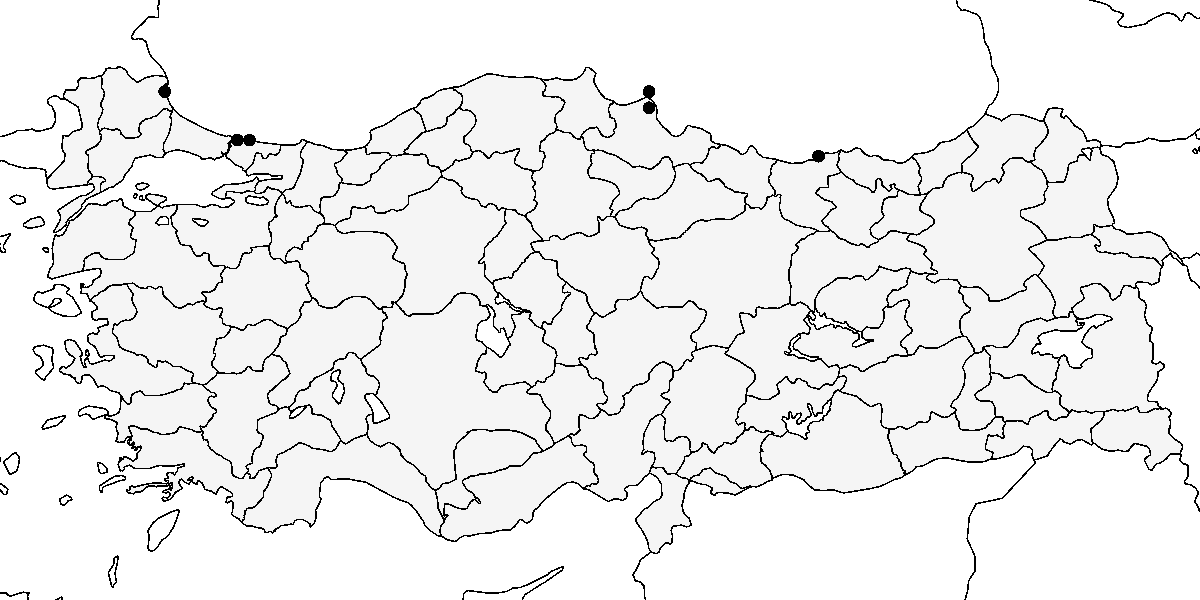
\includegraphics[keepaspectratio]{images/harita_Calcarius lapponicus.png}}

\textbf{Üreme}

Türkiye'de yuvalamaz. Avrasya ve Kuzey Amerika'nın tundra kuşağında
ürer.

\textbf{Alttürler ve Sınıflandırma}

Türkiye'de kaydedilen bireyler büyük olasılıkla nominat alttüre aittir.
Bu takson, Kuzey Norveç'ten Doğu Sibirya'ya kadar olan bölgede ürer
(Byers, Olsson \& Curson, 1995).

\section{Alaca Çinte}\label{alaca-uxe7inte}

\emph{Plectrophenax nivalis}, Snow Bunting

\textbf{\emph{Lokal olarak az sayıda görülen kış konuğudur.}}

Son yıllarda türden toplam sekiz kayıt yapılmış, bunların dördü
Kızılırmak Deltası'ndandır. 1 Şubat 1992'de Balık Gölü'nün hemen
kuzeyinde sekiz birey (Dijksen \& Klemann, 1992), 7 Kasım 1992'de Liman
Gölü çevresinde toplam 46 birey (Kirwan, 1993), 1 Kasım 2004 ve 28 Kasım
2006 tarihlerinde üç birey (Balmer \& Betton, 2007a) gözlenmiştir. Diğer
kayıtlar ise 13 Şubat 2005'te Kulu Gölü'nde, 21 Kasım 2006'da Vize'de,
27 Kasım 2006'da İğneada'da (Balmer \& Betton, 2007a) ve 22 Ekim 2007'de
Vize'de fotoğraflanan bireylerdir.

19. yüzyıldaki kayıtları temel alan (Braun, 1901) ve (Mathey-Dupraz,
1920--24) gibi kaynaklarda, İstanbul Boğazı'nda düzensiz bir kış konuğu
ve geçit kuşu olarak yer verilmiştir (Kasparyan, 1956; Kumerloeve,
1961). Ancak bu değerlendirmeyi destekleyen yalnızca bir örnek
bulunmaktadır. Bu birey, eskiden Robert Kolej'in koleksiyonunda yer
alıyordu (Kirwan, 1997). Görünüşe göre, 1905--1906 kışında İstanbul'daki
kuş pazarlarında da satılmıştır (Braun, 1908).

\pandocbounded{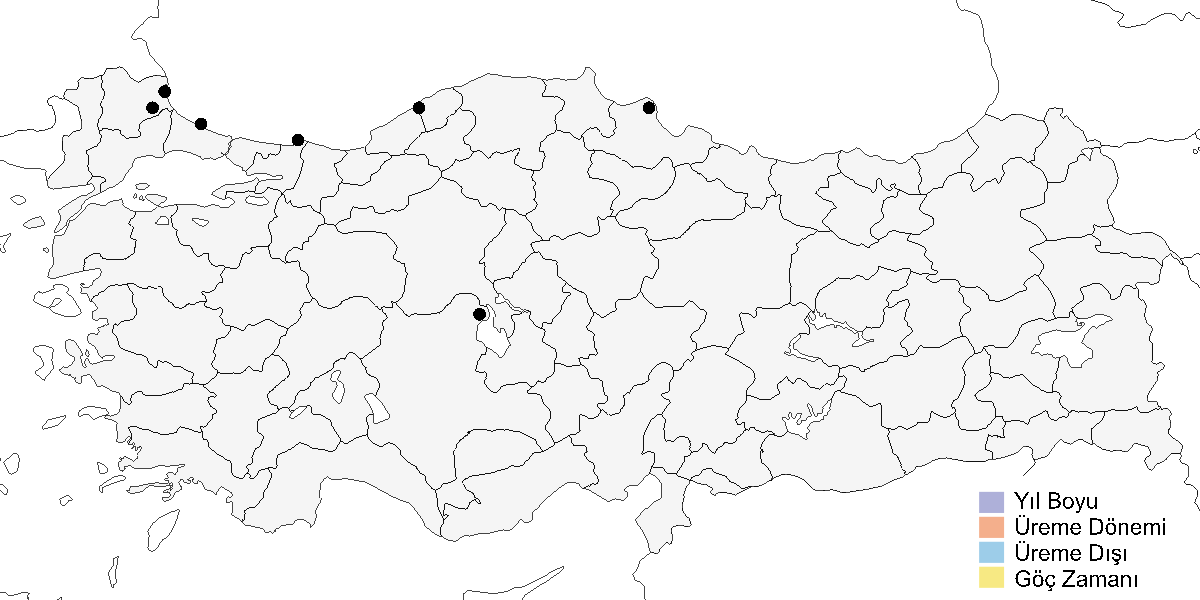
\includegraphics[keepaspectratio]{images/harita_Plectrophenax nivalis.png}}

\textbf{Üreme}

Türkiye'de yuvalamaz. Avrasya ve Kuzey Amerika'nın tundra kuşağında
ürer.

\textbf{Alttürler ve Sınıflandırma}

Türkiye'den toplanmış herhangi bir örnek günümüzde mevcut değildir.
Ancak kaydedilen bireylerin neredeyse kesin olarak \emph{vlasowae}
alttürüne ait olduğu kabul edilebilir. Bu alttür, Kuzeydoğu Avrupa
Rusyası'ndan Sibirya'nın doğusundaki Çukotski Yarımadası'na kadar uzanan
bölgede ürer, kış aylarında güneye göç eder ve batıda Macaristan ile
Romanya'ya kadar ulaşır (Byers \emph{vd.}, 1995).

\section{Kara Başlı Çinte}\label{kara-baux15flux131-uxe7inte}

\emph{Emberiza melanocephala}, Black-headed Bunting

\textbf{\emph{Yaygın olarak çok sayıda bulunan yaz göçmenidir.}}

Mayıs ve temmuz arasında hububat tarlalarının en yaygın kuşlarındandır.
Her türlü tarım alanı ve çalılıklarda üreyen tipik bir türdür.
Genellikle 2400 metre altındaki alanlarda görülse de, yer yer 2900
metreye kadar ve göç sırasında daha yüksek irtifalarda da
kaydedilmiştir. Karadeniz Bölgesi'nin büyük bölümünde, özellikle Doğu
Karadeniz'de üremez. Üreme alanlarına Güneydoğu Anadolu, Akdeniz ve
Ege'de nisan ortasında, orta ve kuzey bölgelerde ise genellikle mayıs
başında ulaşır.

En azından mayıs ortasına kadar Türkiye'nin kuzey ve batısında üreyen
bireylerin geçişi sürer. En erken 28 Mart'ta iki gözlem kaydedilmiştir.
Göç sırasında genellikle küçük gruplar hâlinde, bazen yüzlerce bireyden
oluşan sürüler halinde görülür. Erkeklerin daha erken vardığı
düşünülmektedir. Geri dönüş ağustos sonunda başlar ve eylül sonunda
tamamlanır. En geç kayıt 31 Ekim'de Van Gölü'nden bildirilmiştir.

\pandocbounded{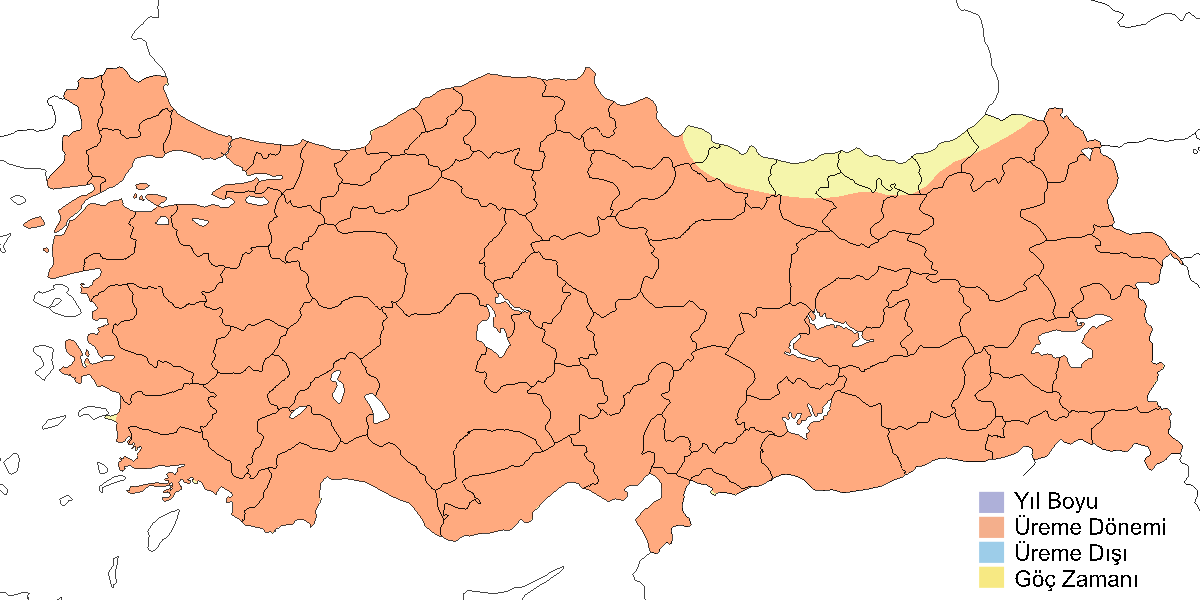
\includegraphics[keepaspectratio]{images/harita_Emberiza melanocephala.png}}

\textbf{Üreme}

\textbf{Yuvalama alanı:} Çoğunlukla tarlaların sınırındaki sık
çalılıklar, makilikler ve çitlerde, ayrıca bahçeler, meyve bahçeleri,
açık ormanlar ve geniş tarlaların yabani otlarla kaplı kenarlarında
ürer.\\
\textbf{Yuvası:} Yuvasını bir çalı, küçük bir ağaç, yabani ot,
devedikeni veya sık orman altı bitki örtüsüne, genellikle yerden
0,5--1,0 m yüksekliğe yapar; en yüksek yuva 2,5 m yüksekliktedir. Bitki
gövdeleri ve kuru yapraklardan kâse şeklinde yaptığı yuvasını daha ince
otlar ve kılla astarlar.\\
\textbf{Yumurta sayısı:} Türkiye'de üç yumurtalı yedi yuva, dört
yumurtalı yirmi sekiz yuva ve beş yumurtalı on iki yuva kaydedilmiştir.
Bunların dışındaki yuvalarda yumurtalar henüz tamamlanmamıştır. Ayrıca,
bir yuvada üç yavru, altı yuvada dört yavru ve beş yuvada beş yavru
sayılmıştır.\\
\textbf{Üreme dönemi:} Üreme genellikle mayıs başı ile ortasında başlar.
Diğer bölgelerinde olduğu gibi Türkiye'de de muhtemelen yılda iki kez
kuluçkaya yatar. \textbf{MAR:} 6 Haziran 1966'da Manyas Gölü'nde dört
yumurtalı bir yuva bulunmuş, 19 Haziran 1973'te yiyecek taşıyan
erişkinler ve 25 Haziran 1973'te Kösedere'de yeni tüylenmiş yavrular
gözlenmiştir. \textbf{EGE:} 23 Nisan 2003'te Altınkum'da çok az kuş
varken, 3 Mayıs'ta sayıları yüzleri bulan öten ve kurlaşan bireyler
gözlenmiş, 4 Mayıs'ta yarısı tamamlanmış bir yuva, 8 Mayıs'ta ise aynı
yuvada iki yumurta bulunmuştur. Ege'nin diğer bölgelerinde mayıs ayında
toplam 21 yuva kaydedilmiş, bunların en erkeni 7 Mayıs'ta yumurtaları
tamamlanmamış bir yuvadır. 19 Mayıs 1950'de içinde Guguk yumurtası olan
bir yuva (McNeile, 1950, 1951, 1954, 1967, 1968, 1970, 1972, 1973) ve
mayıs sonunda içinde küçük yavrular olan dört yuva bulunmuştur.
\textbf{AKD:} 2 Mayıs 1970'te Amik Gölü'nde yuva yapımı, 15 Mayıs
2004'te yapım aşamasında iki yuva, 13 Mayıs 2004'te tamamlanmış bir
yuvada ise henüz yumurta bulunmamıştır. Demirkazık'ta mayıs ortası ile
haziran ortası arasında sekiz yuvada yumurtalar, haziran ortasında yeni
çıkmış yavrular ve 10 Haziran--temmuz arasında tüylenmiş yavrular
kaydedilmiştir. \textbf{KAD.} 26 Haziran 1986'da aile grupları
kaydedilmiştir. \textbf{İÇA:} Mayısın son haftasında beş, haziranın ilk
yarısında altı yuvada yumurta görülmüş, 10 Haziran 1988'de yuva yapımı,
ağustos başında ise tüylenmiş yavrular ve eşlik eden erişkinler
gözlenmiştir. \textbf{DOA:} Haziranın ilk yarısında içinde yumurta olan
dört yuvadan en erkeni 5 Haziran 2001 tarihindedir. \textbf{GDA:} 5
Mayıs 1992'de Halfeti'de, 3 Haziran 2001 ve 10 Mayıs 2004'te
Gaziantep'te, 11 Mayıs 2004'te Birecik'te yuva yapımı kaydedilmiştir. 7
Mayıs 1970'te Birecik'te dört yumurtalı bir yuva, 17 Mayıs 2004'te
Işıklı ve Durnalık'ta iki yuvada yumurtalar, haziranın ilk yarısında ise
beş yuvada yumurta ve 3 Haziran 2001'de Yeşilce'de dört küçük yavru
kaydedilmiştir. 6--12 Haziran 2006'da dört yuvada yavru, 12 Haziran
1996'da tüylenmiş yavrular ve 14 Haziran'da uçan yavrular gözlenmiştir.

\textbf{Alttürler ve Sınıflandırma}

Monotipik bir türdür.

\section{Kızıl Başlı Çinte}\label{kux131zux131l-baux15flux131-uxe7inte}

\emph{Emberiza bruniceps}, Red-headed Bunting

\textbf{\emph{Rastlantısal konuktur.}}

7 Eylül 2012 tarihinde Rize sahilinde 1 birey E. Yoğurtçuoğlu tarafından
kaydedilmiştir.

\pandocbounded{\includegraphics[keepaspectratio]{images/harita_Emberiza bruniceps.png}}

\textbf{Üreme}

Türkiye'de yuvalamaz. Orta Asya'da yuvalar, kışı Hindistan'da geçirir.

\textbf{Alttürler ve Sınıflandırma}

Monotipik bir türdür.

\section{Tarla Çintesi}\label{tarla-uxe7intesi}

\emph{Emberiza calandra}, Corn Bunting

\textbf{\emph{Yaygın olarak çok sayıda bulunan yerli ve kış
göçmenidir.}}

Tarım arazileri, çalılık yarı bozkırlar ve benzeri açık alanlarda 2300
metreye kadar çok sayıda bulunur. Yer yer çok yoğun olarak ürediği İç ve
Doğu Anadolu'da yarı göçmendir. Karadeniz ve Güneydoğu Anadolu'da ise
nispeten lokaldir; Güneydoğu'da uygun habitatların sayısı muhtemelen
artmaktadır. Kızılırmak Deltası'nda 1500--2000 çiftin ürediği tahmin
edilse de Karadeniz Bölgesi'nin kalanında çok daha az sayıda olduğu
açıktır.

Üreme sonrası ağustos sonu ile ekim arasında yüzlerce bireyden oluşan ve
bazen 1000'i aşan kalabalık sürüler oluşturur. Ayrıca ülke dışından da
göç alır. Diğer yandan göç gözlem noktalarında geçit yaptığı
görülmemiştir. Orta Doğu'nun diğer bölgelerinde kışlamak üzere güneye
doğru göç eden kalabalık sürüler, sonbahar sonunda güney kıyılarında
gözlenebilir. Kış aylarında çoğunlukla ülkenin batı ve orta bölgelerinde
bulunur. 21 Ocak 1992'de Aksaray Eşmekaya'da 1500 bireyden oluşan büyük
bir sürü kaydedilmiştir.

\pandocbounded{\includegraphics[keepaspectratio]{images/harita_Emberiza calandra.png}}

\textbf{Üreme}

\textbf{Yuvalama alanı:} Çoğunlukla buğday ve diğer hububat tarlaları,
çayırlar ve açık çalılık arazilerde, ara sıra çitler ve seyrek ağaçlı
arazilerde ürer.\\
\textbf{Yuvası:} Yere yapılan yuvalar boylanan ekin veya bir çalının
gölgesinde bulunur (3 yuva); yerden yüksekteki yuvalar ise bir çalıya ya
da karmaşık otların arasındaki bir çalıya kurulur (7 yuva). Yerden
yüksekte yuva bulma olasılığı daha yüksek olsa da, çoğunluğun yerde
yuvaladığı düşünülmektedir. Yuva kâse şeklindedir, otlarla örülür ve
daha ince otlar, kökler ve kılla astarlanır.\\
\textbf{Yumurta sayısı:} Türkiye'de iki yuvada dört, bir yuvada beş ve
altı yuvada altı yumurta kaydedilmiştir. Ayrıca, bir yuvada üç, bir
yuvada altı yavru sayılmıştır.\\
\textbf{Üreme dönemi:} Üreme alanlarında nisan ortasından itibaren gelir
ve hemen yumurta koyar. \textbf{MAR:} 1993'te Kocaçay Deltası'nda tuzcul
ovada hektarda 0,76 çift, nadasa bırakılmış tarım arazilerinde hektarda
0,43 çift, tarımsal araziler ve kumullarda daha düşük yoğunlukla ürediği
tespit edilmiştir (Ertan, 1996). 8 Haziran 1966'da Bandırma yakınında
içinde dört yumurta ve iki yavru bulunan bir yuva, 25 Nisan 1966'da
dörtte üçü tamamlanmış başka bir yuva bulunmuştur. \textbf{KAD.}
Kızılırmak Deltası'nda 1992'de kurak çayırlar, tarlalar ve çok seyrek
bitkili kumullarda 100 hektarda 35--50 çiftlik bir yoğunluk
hesaplanmıştır. İlk yumurtalı yuva 17 Mayıs'ta görülmüş, 1 Haziran'dan
itibaren yiyecek taşıyan birçok erişkin kaydedilmiştir (Hustings \&
Dijk, 1994). Türkiye dışında yılda iki kez kuluçkaya yattığı
bilinmektedir. Bu nedenle Türkiye'de temmuz ve sonrasında yeni tüylenmiş
yavru kaydının olmaması dikkat çekicidir. \textbf{EGE:} Altınkum'da 20
Nisan 2002'de altı yumurtalı iki yuva, 24 Nisan 2002'de yavrulu bir yuva
görülmüş ve ilk yumurtlama tarihinin 6 Nisan olduğu anlaşılmıştır. 3
Mayıs 2001'de bir yuvada yaklaşık beş günlük yavrular, 24 ve 29 Mayıs
2004'te altışar yumurtalı yuvalar kaydedilmiştir. Her iki yuva da yerden
0,8 m yüksekteki çalılardadır. 20 Nisan 1951'de İzmir yakınlarında üç
yumurtalı ve henüz kuluçkaya yatılmamış bir yuva 24 Nisan'da altı
yumurtaya tamamlanmış, 26 Nisan'da dört yumurtalı ikinci bir yuva
kuluçkanın ileri evresindeyken bulunmuştur (McNeile, 1950, 1951, 1954,
1967, 1968, 1970, 1972, 1973). \textbf{AKD:} Göksu Deltası'nda 5 Mayıs
2004'te iki yumurtalı, 16 Mayıs 2004'te beş yumurtalı bir kuluçka
gözlenmiştir. \textbf{GDA:} 20 Mayıs 2007'de Birecik'te bir çalının
içindeki yuvada dört yumurta, 11 Haziran 1996'da Halfeti'de dört
tüylenmiş yavru gözlenmiştir. \textbf{İÇA:} Şubat sonundan mart ortasına
kadar üreme alanlarına varan bireylerde erkeklerin ötüşü mart ile temmuz
arasında, bazen de ekimde duyulur (Wadley, 1951). \textbf{DOA:}
Erzurum'da 1911--12 döneminde kuşlar üreme alanlarına nisan sonunda
varmış, ağustos başında ayrılmıştır (McGregor, 1917).

\textbf{Alttürler ve Sınıflandırma}

Ülkenin neredeyse tamamında nominat \emph{calandra} alttürü bulunur.
Güneydoğu Anadolu'da, özellikle Fırat ile Ceylanpınar arasındaki bölgede
\emph{buturlini} alttürünün varlığı olasıdır (Byers \emph{vd.}, 1995;
Roselaar, 1995). Ancak tür içindeki coğrafi varyasyonlar genellikle
düşük ve klinal yapıdadır; bu nedenle diğer alttürlerin geçerliliği
tartışmalıdır(Vaurie, 1956). Tür, eski kaynaklarda \emph{Miliaria} cinsi
altında sınıflandırılmıştır.

\section{Kaya Çintesi}\label{kaya-uxe7intesi}

\emph{Emberiza cia}, Rock Bunting

\textbf{\emph{Nispeten yaygın olarak genellikle çok sayıda bulunan yerli
veya yarı göçmendir.}}

Dağlık arazilerde, kayalık ve çalılarla kaplı, bazen seyrek ağaçlı
yamaçlarda görülür. Ayrıca Doğu Karadeniz Dağları'nda özellikle açık
kızılçam (Pinus brutia) ormanlarında da bulunur. Üreme sezonunda
genellikle 800 ile 2600 metre arasında, nadiren daha alçakta, örneğin
Karadeniz Bölgesi'nde 500 metrede ve Toroslar'da 600 metrede
kaydedilmiştir. Trakya'da çok lokal olarak, İç Anadolu bozkırında
yalnızca güneydeki izole dağlarda ve Güneydoğu Anadolu'nun yalnızca
kuzeybatı ucunda üreme döneminde bulunur. Batı bölgelerde nispeten
seyrektir. Kış aylarında daha yaygın hale gelir, deniz seviyesine kadar
iner ve çoğunlukla batı ve güney bölgelerde kışlar.

\pandocbounded{\includegraphics[keepaspectratio]{images/harita_Emberiza cia.png}}

\textbf{Üreme}

\textbf{Yuvalama alanı:} Özellikle kireçtaşı zeminli, ağaç ve bodur
ağaçların bulunduğu kayalık yamaçlarda, açık ormanlarda ve vadilerde
yuvalar. Kızılcahamam'da orman açıklıkları, bozuk meşelikler ve kayalık
yamaçlar tercih edilir (Barış \emph{vd.}, 1984).\\
\textbf{Yuvası:} Yerde, kısmen bir çalı, bodur ağaç veya kaya
gölgesindedir. Bazen hafif oyuklar, yarlar veya duvarlardaki girintiler
kullanılır. Yuva kâse şeklindedir, ağırlıkla otlardan örülür, daha ince
otlar, kökçükler ve biraz kılla astarlanır.\\
\textbf{Yumurta sayısı:} Türkiye'de iki yuvada dört yumurta
kaydedilmiştir.\\
\textbf{Üreme dönemi:} Mayıs ayından itibaren yumurta koyar. Yavrular
haziran sonrası gözükür. \textbf{İÇA:} 7 Haziran 1977'de Kızılcahamam'da
bir yuvada dört yumurta görülmüştür (Pforr \& Limbrunner, 1982). 28
Nisan 1901'de İzmir'de bir taşın altındaki yuvada dört yumurta tespit
edilmiş ve örnekleri Manchester Müzesi'ne alınmıştır. \textbf{AKD:}
17--23 Temmuz 1971'de Torosdağı'nın kuzey yamaçlarında 1700--2500 m
arasında birçok çiftin yavrularını beslediği görülmüş, 19 Haziran
1996'da Sertavul Geçidi'nde bir çift üç tüylenmiş yavruyu beslemiştir.
Bu kayıt, ilk yumurtanın yaklaşık 22 Mayıs'ta bırakıldığını
göstermektedir. 13 Mayıs 2005'te aynı bölgede sıradışı bir yuva, küçük
bir çam ağacının yerden 1 m yükseklikteki gövdesine yakın bir dalda
bulunmuş; yuvada yumurtadan yeni çıkmış üç yavru ve henüz çatlamamış bir
yumurta tespit edilmiştir. Bu gözlem, ilk yumurtanın nisan sonunda
bırakıldığını düşündürmektedir. \textbf{DOA:} 9 Temmuz 1985'te Nemrut
Dağı'nda (Tatvan) bir aile grubu ve uyarı sesi çıkararak yiyecek taşıyan
bir çift, 18 Mayıs 2006'da Van Çatak'ın kuzeyindeki Yenimahalle'de
yiyecek taşıyan bir çift gözlenmiştir.

\textbf{Alttürler ve Sınıflandırma}

Taksonomik durumu karmaşıktır ve revizyona açıktır. Kuzey Anadolu ve
Trakya boyunca nominat \emph{cia}, Güney Anadolu'da en azından
İzmir--Hatay hattında \emph{hordei} alttürlerinin bulunduğu
bildirilmiştir (Roselaar, 1995). Doğu Anadolu'nun doğusundan gelen
tahnit örnekleri \emph{prageri} veya \emph{prageri} ile \emph{par}
alttürlerinin ara formu olarak sınıflandırılmıştır. Ülkenin geri
kalanındaki popülasyonlar ise alttür düzeyinde net olarak
tanımlanamamıştır (Roselaar, 1995). Diğer yazarlar \emph{prageri}'yi
\emph{par}'ın bir sinonimi, \emph{hordei}'yi ise nominat formun içine
dâhil etmiş, Güney Avrupa, Balkanlar ve Türkiye'deki kuşlar için
kullanılan \emph{barbata} alttürünü ise geçerli saymamışlardır (Vaurie,
1956; Byers \emph{vd.}, 1995).

Tring Doğa Tarihi Müzesi'ndeki Türkiye kökenli ve \emph{hordei} olarak
tanımlanan tahnitler, Roselaar tarafından belirtilen tüm karakterlere
göre incelenmiş, ancak nominat \emph{cia} alttürüne son derece benzer
olduğu görülmüştür. Bu nedenle \emph{hordei} geçerli bir takson olarak
kabul edilmemektedir. \emph{Prageri} örnekleri incelenememiş olsa da,
\emph{par} alttürüne ait olduğu düşünülen örnekler de bu iki formun
geçerliliğini ciddi şekilde sorgulatmaktadır.

\section{Bahçe Çintesi}\label{bahuxe7e-uxe7intesi}

\emph{Emberiza cirlus}, Cirl Bunting

\textbf{\emph{Yaygın olarak çok sayıda bulunan yerlidir.}}

Batı Karadeniz, Marmara ve Ege Bölgesi'nin kuzey ve iç kesimlerinde
yaygın ancak muhtemelen eskisi kadar bol olmayan yerli bir türdür. Güney
Ege'de nadirdir. Kalan bölgelerde ise daha lokal dağılım gösterir; İç
Anadolu ve Toroslar'ın alçak kesimlerinde seyrek olarak bulunur. Üreme
döneminde, alçak irtifadaki makilikler, sık çalılıklar, ormanlık
alanlar, baltalıklar ve meşeliklerde görülse de, en sık bulunduğu
habitat çalılık ormanlarla kaplı alçak tepelerdir. Bu habitatlar
Türkiye'de kuş gözlemcilerinin ilgisini nadiren çektiğinden, türün
gerçek durumu belirsizdir. Ara sıra kış aylarında ve muhtemelen göç
dönemlerinde az sayıda birey Akdeniz Bölgesi'nde de gözlenmiştir.
Görünüşe göre, bu bölgede eskiden daha yaygındı.

\pandocbounded{\includegraphics[keepaspectratio]{images/harita_Emberiza cirlus.png}}

\textbf{Üreme}

\textbf{Yuvalama alanı:} Orman, orman kenarı, zeytinlikler ve yol
kenarındaki çalılar, bodur ağaçlar ve çitlerde yuvalar. Çoğunlukla
tepelik alanlarda bulunur, ancak çalı bulunduğu sürece ova ve
düzlüklerde de ürer. Kocaçay Deltası'nda alüvyal ormanın açık ve kurak
kısımlarında ve tarım arazilerinde çok sayıda ürediği belirlenmiştir.
1993'te yapılan bir çalışmada alüvyal ormanda üreme yoğunluğu hektarda
0,39 çift, kurak ve çeşitçe zengin tarım arazilerinde ise hektarda 1,2
çift olarak bulunmuştur (Ertan, 1996).\\
\textbf{Yuvası:} Yuva ot, yosun ve köklerden oluşan muntazam bir
kâsedir, kıl ve otlarla astarlanır. Beş yuva yerden 0,7--1,6 m yüksekte,
çoğunlukla çalılar üzerinde ve bir örnekte budanarak bodur kalmış bir
çamda bulunmuştur (McNeile, 1950, 1951, 1954, 1967, 1968, 1970, 1972,
1973).\\
\textbf{Yumurta sayısı:} Türkiye'de bir yuvada üç yumurta, iki yuvada
dört yumurta, iki yuvada beş yumurta ve bir yuvada altı yumurta
kaydedilmiştir. Ayrıca içinde iki yumurta bulunan bir yuvanın kuluçkası
tamamlanmamış olarak değerlendirilmiştir. Bir yuvada üç yavru, bir
yuvada ise dört yavru sayılmıştır.\\
\textbf{Üreme dönemi:} Nisan ve mayıs ayında yumurta koyar. yavrular
haziran sonuna kadar kaydedilir. \textbf{MAR:} 3 Haziran 2006'da Kocaçay
Deltası'nda üç yumurtalı bir yuva bulunmuş, 14 Haziran 1966'da Çatal
Dağ'da ve 11 Haziran 1969'da Çamlıca'da yiyecek taşıyan erişkinler
gözlenmiştir. 18 Haziran 1973'te Kilyos'ta birçok erişkinin yiyecek
taşıdığı, 21 Haziran 1973'te Vize'de tüylenmiş yavrular ve 17 Haziran
1973'te Bebek'te yeni tüylenmiş yavrular kaydedilmiştir. Bu son gözlem,
yumurtlamanın 21 Mayıs civarında gerçekleştiğini göstermektedir.
\textbf{EGE:} 3 Nisan 1984'te Bafa Gölü'nde yuva yapımı gözlenmiş, 30
Nisan 2003'te içinde dört tane neredeyse tüylenmiş yavru bulunan bir
yuva, yumurtlamanın nisan başında gerçekleştiğini göstermiştir. 1950,
1951 ve 1954'te İzmir'de toplam yedi yuva bulunmuştur (McNeile, 1950,
1951, 1954, 1967, 1968, 1970, 1972, 1973). Bu yuvalardan bazıları ikinci
kuluçkaya ait olabilir. 22 Mayıs 1950'de iki yumurtalı, 15 Mayıs 1951'de
kuluçkaya yeni yatılmış beş yumurtalı, 26 Mayıs 1951'de altı yumurtalı,
28 Mayıs 1951'de dört ve beş yumurtalı iki yuva, yine aynı gün
kuluçkanın son evresindeki dört yumurtalı bir yuva, 27 Mayıs 1954'te ise
tüyleri çıkmış yavruların bulunduğu bir yuva kaydedilmiştir.
\textbf{AKD:} 22 Mayıs 1989'da Çamiçi'nde tüylenmiş yavrular, 15 Temmuz
2004'te ise bir genci besleyen bir erkek gözlenmiştir. \textbf{KAD.}
Temmuz 1966'da Gerze'de 3--5 aile grubu ve 9 Haziran 1975'te yavrularını
besleyen erişkinler gözlenmiştir. \textbf{İÇA:} 6 Mayıs 1993'te
Kızılcahamam'da üç yeni çıkmış yavrunun bulunduğu bir yuva,
yumurtlamanın yaklaşık 20 Nisan'da başladığını göstermektedir.

\textbf{Alttürler ve Sınıflandırma}

Monotipik bir türdür (Svensson, 1992).

\section{Sarı Çinte}\label{sarux131-uxe7inte}

\emph{Emberiza citrinella}, Yellowhammer

\textbf{\emph{Çok lokal olarak yaz konuğu, yaygın olarak az sayıda kış
konuğudur.}}

Trakya'nın kuzeyinde ürediği bildirilmiş(Özkan, 2010), burada az sayıda
yerli olduğu tahmin edilmektedir; ancak bu bilginin teyit edilmesi
gerekmektedir. Üreme döneminde genellikle dağlık bölgelerdeki
çalılıklarda ve parçalanmış karışık ormanlarda, orta irtifalarda
bulunur. Akdeniz Bölgesi'nde Orta ve Batı Toroslar'da (Deppe, 1990;
Kirwan \& Martins, 1994) ve Güney Marmara'da (OST, 1975; Martins, 1989)
üreme ihtimali vardır.

Geçit kuşu olarak Türkiye genelinde, kış konuğu olarak ise ekim başından
mart sonuna ve nisan başına kadar Trakya, Batı ve Orta Anadolu'da yaygın
ancak çok bol olmayacak şekilde görülür. Öncelikle bir kış konuğu olup,
üreme durumu ve yayılışı ayrıntılı olarak bilinmemektedir. Kışlaklarda
en erken 6 Ekim'de, en geç 18 Nisan'da kaydedilmiştir. Doğu Anadolu'da
birkaç göçmen birey gözlenmiş, Malatya ve Elazığ çevresinde ise
kışladığı bilinmektedir.

\pandocbounded{\includegraphics[keepaspectratio]{images/harita_Emberiza citrinella.png}}

\textbf{Üreme}

\textbf{Yuvalama alanı:} Trakya'da potansiyel üreme habitatı açık
ağaçlık alanlar ve çalılıklardır.\\
\textbf{Yuvası:} Türkiye'de yuva ile ilgili bir kayıt bulunmamaktadır.\\
\textbf{Yumurta sayısı:} Türkiye'de yumurta veya yavruya dair doğrudan
bir gözlem yapılmamıştır.\\
\textbf{Üreme dönemi:} Mayıs ve haziran ayında yumurta koymaya başlar.
\textbf{MAR:} Mayıs ve haziran aylarında Istranca Dağları'nda öten
erkekler tespit edilmiştir.

\textbf{Alttürler ve Sınıflandırma}

Üreyen kuşlar incelenmemiş olsa da, tüm kayıtların görünüşe göre
\emph{erythrogenys} alttürüne ait olduğu düşünülmektedir (Roselaar,
1995). Bu alttürde, ak başlı çintede görülen bazı karakterler de
bulunur. Bunun, iki tür arasında uzun bir zaman dilimine yayılan
melezleşme ve gen akışı sonucu oluştuğu ileri sürülmüştür (Byers
\emph{vd.}, 1995; Panov, Roubtsov \& Monzikov, 2003).

\section{Ak Başlı Çinte}\label{ak-baux15flux131-uxe7inte}

\emph{Emberiza leucocephalos}, Pine Bunting

\textbf{\emph{Rastlantısal konuktur.}}

İlk kez, 13 Mart 1974'te Ankara'da Ortadoğu Teknik Üniversitesi
Yerleşkesi'nde 3 erkek ve 3 dişi görülmüştür (Beaman, 1986; Kasparek,
1986). 2 Şubat 1997'de aynı yerde biri erkek olan beş kuş kaydedilmiştir
(Kirwan \emph{vd.}, 2003). Sonraki kayıtlar şu şekildedir: 30 Kasım
2005'te Afyon'da Sandıklı ile Kızılören arasında bir erkek ve 10--16
Ocak 2008'de erişkin bir dişi fotoğraflanmıştır. 10 Ocak 2008'de
İstanbul Büyükçekmece Gölü Mimarsinan mevkiinde 1 birey gözlenmiştir (F.
Can). 30 Ocak 2008'de Malatya üzerinden ``Trabzon to Gaziantep''
rotasında 1 birey bulunmuştur (M. Erturhan). 31 Ocak 2011'de Kayseri
Yahyalı--Mustafabeyli yolu üzerinde 1 birey kaydedilmiştir (\emph{M.
Ünlü}). 15 Mart 2011'de Iğdır Aras Kuş Halkalama İstasyonu'nda 1 birey
gözlenmiştir. 25 Ocak 2016'da Kayseri Çiğilli Mahallesi'nde 1 birey
bulunmuştur (\emph{M. Ünlü}). 30 Ekim 2017'de Iğdır Aras Kuş Halkalama
İstasyonu'nda 1 birey gözlenmiş, 2 Mart 2018'de 1 birey kaydedilmiştir
(\emph{B. Demir}). 14 Şubat 2019'da Bolu Çoğullu Köyü Ulusu bölgesinde 5
birey kaydedilmiştir (N/A). 28 Mart 2019'da Iğdır Aras Kuş Halkalama
İstasyonu'nda 1 birey kaydedilmiştir. 17 Mart 2020'de aynı istasyonda
yine 1 birey gözlenmiştir. 25 Şubat 2021'de Gaziantep Sof Dağı genel
alanında 1 birey gözlenmiştir (\emph{G. Güzelbey}). 26 Ekim 2021'de
Samsun Kızılırmak Deltası Kuş Cenneti'nde 1 birey kaydedilmiştir
(\emph{E. Yoğurtçuoğlu}). 18 Ekim 2022'de Trabzon Kıyıcık--Yeniköy
Deresi Ağzı'nda 1 birey gözlenmiştir (\emph{E. Yoğurtçuoğlu}). 18 Kasım
2022'de Hakkâri Bölük Köyü--Yüksekova'da 1 birey kaydedilmiştir
(\emph{E. Bıyıkoğlu; E. Kayhan}). 11 Mart 2023'te Iğdır Aras Kuş
Halkalama İstasyonu'nda 1 birey bulunmuştur (\emph{K. Derneği; D.
Kitel}). 1 Kasım 2023'te Ankara Bolu Yolu üzerinde 1 birey gözlenmiştir
(\emph{O. Aydın}). 8 Mart 2024'te Çorum Çatak'ta isimsiz bir yol
üzerinde 1 birey kaydedilmiştir (\emph{E. Bıyıkoğlu}).

Hepsi 19. yüzyılda, çoğu 1861 ile 1871 arasında İstanbul'da kalan T.
Robson tarafından toplanmış toplam 6 örnek vardır. Liverpool Müzesi'nde
(National Museum and Galleries on Merseyside) T11583 numarasıyla kayıtlı
olan bir erkek, 1858 kışında bilinmeyen bir tarihte İstanbul'da H.
Loftus tarafından toplanmış, bir müddet Canon Tristram'ın koleksiyonunun
bir parçası olmuştur. 31 Ekim 1865'te İstanbul Ortaköy'de toplanan bir
erkek, şu anda Tring Doğa Tarihi Müzesi'nde bulunmaktadır (NHM
88.9.1912.524). Bunun dışında iki erişkin erkek 1869'da Robson
tarafından toplanmış ve Dresser'e yollanmış, şimdi Manchester Müzesi'nde
bulunmakta olup BB03154 numaralı kuş 21 Ekim'de ``Konstantinopolis
yakınındaki Kâğıthane tepelerinde'', BB03153 numaralı kuş ise 8 Kasım'da
``Konstantinopolis'te'' toplanmıştır. Biri dişi olan iki örnek, tahminen
Mathey-Dupraz tarafından kaydedilenler olup İstanbul Robert Koleji'nin
koleksiyonunda bulunmaktadır. Bu kuşlar, müzedeki çoğu kuş gibi
muhtemelen yakın çevreden toplanmış olsalar da toplanma tarihi ve yeri
hakkında bilgi bulunmamaktadır. Robson'un yorumlarına göre bu tür yıldan
yıla sonbahar geçişinde görülse de 19. yüzyıl yazarları türü seyrek kış
konuğu olarak sınıflandırmıştır.

İlk kez, 13 Mart 1974'te Ankara'da Ortadoğu Teknik Üniversitesi
Yerleşkesinde 3 erkek ve 3 dişi (Beaman, 1986; Kasparek, 1986), 2 Şubat
1997'de aynı yerde biri erkek olan beş kuş (Kirwan \emph{vd.}, 2003)
görülmüştür

Sonraki kayıtları şu şekildedir. 30 Kasım 2005'te Afyon'da Sandıklı ve
Kızılören arasında bir erkek ve 10-16 Ocak 2008'de erişkin bir dişi
fotoğraflanmıştır. 10 Ocak 2008'de İstanbul Büyükçekmece Gölü Mimarsinan
mevkiinde 1 birey \emph{F. Can} tarafından gözlendi. 30 Ocak 2008'de
Malatya üzerinden ``Trabzon to Gaziantep'' rotasında 1 birey \emph{M.
Erturhan} tarafından bulundu. 31 Ocak 2011'de Kayseri
Yahyalı--Mustafabeyli yolu üzerinde 1 birey \emph{M. Ünlü} tarafından
kaydedildi. 15 Mart 2011'de Iğdır Aras Kuş Halkalama İstasyonu'nda 1
birey \emph{Ç. H. Şekercioğlu} tarafından gözlendi. 25 Ocak 2016'da
Kayseri Çiğilli Mahallesi'nde 1 birey \emph{M. Ünlü} tarafından
kaydedildi. 30 Ekim 2017'de Iğdır Aras Kuş Halkalama İstasyonu'nda 1
birey \emph{B. Demir} tarafından gözlendi. 2 Mart 2018'de aynı
istasyonda 1 birey yine \emph{B. Demir} tarafından kaydedildi. 14 Şubat
2019'da Bolu Çoğullu Köyü Ulusu bölgesinde 5 birey \emph{NA} tarafından
gözlendi. 28 Mart 2019'da Iğdır Aras Kuş Halkalama İstasyonu'nda 1 birey
\emph{J. Ramírez} tarafından kaydedildi. 17 Mart 2020'de aynı istasyonda
yine 1 birey \emph{J. Ramírez} tarafından kaydedildi. 25 Şubat 2021'de
Gaziantep Sof Dağı genel alanında 1 birey \emph{G. Güzelbey} tarafından
gözlendi. 26 Ekim 2021'de Samsun Kızılırmak Deltası Kuş Cenneti'nde 1
birey \emph{E. Yoğurtçuoğlu} tarafından kaydedildi. 18 Ekim 2022'de
Trabzon Kıyıcık -- Yeniköy Deresi Ağzı'nda 1 birey yine \emph{E.
Yoğurtçuoğlu} tarafından gözlendi. 18 Kasım 2022'de Hakkari Bölük
Köyü--Yüksekova'da 1 birey \emph{E. Bıyıkoğlu} ve \emph{E. Kayhan}
tarafından kaydedildi. 11 Mart 2023'te Iğdır Aras Kuş Halkalama
İstasyonu'nda 1 birey \emph{K. Derneği} ve \emph{D. Kitel} tarafından
bulundu. 1 Kasım 2023'te Ankara Bolu Yolu üzerinde 1 birey \emph{O.
Aydın} tarafından gözlendi. 8 Mart 2024'te Çorum Çatak'ta isimsiz bir
yol üzerinde 1 birey \emph{E. Bıyıkoğlu} tarafından kaydedildi.

Görünüşe göre hepsi 19. yüzyılda, çoğu 1861 ile 1871 arasında
İstanbul'da kalan T. Robson tarafından toplanmış toplam 6 örnek vardır.
Liverpool Müzesi'nde (National Museum and Galleries on Merseyside)
T11583 numarasıyla kayıtlı olan bir erkek, 1858 kışında bilinmeyen bir
tarihte İstanbul'da H. Loftus tarafından toplanmış, bir müddet Canon
Tristram'ın koleksiyonun bir parçası olmuştur. 31 Ekim 1865'te İstanbul
Ortaköy'de toplanan bir erkek, şu anda Tring Doğa Tarihi Müzesinde
bulunmaktadır (NHM 88.9.1912.524). Bunun dışında iki erişkin erkek
1869'da Robson tarafından toplanmış ve Dresser'e yollanmış ve şimdi
Manchester Müzesi'nde bulunmakta olup BB03154 kayıt numaralı kuş 21
Ekim'de 'Konstantinopolis yakınındaki Kâğıthane tepelerinde ve BB03153
kayıt numaralı kuş 8 Kasım'da 'Konstantinopolis'te toplanmıştır. Biri
dişi olan iki örnek, tahminen (Mathey-Dupraz, 1920--24) tarafından
kaydedilenler olup İstanbul Robert Kolej'in koleksiyonunda bulunmaktadır
(Kirwan, 1997). Bu kuşlar, müzedeki çoğu kuş gibi muhtemelen yakın
çevreden toplanmış olsalar da toplanma tarihi ve yeri hakkında bilgi
bulunmamaktadır. Robson'un yorumlarına göre bu tür yıldan yıla sonbahar
geçişinde görülse de 19. yüzyıl yazarları türü seyrek kış konuğu olarak
sınıflandırmıştır.

\pandocbounded{\includegraphics[keepaspectratio]{images/harita_Emberiza leucocephalos.png}}

\textbf{Üreme}

Türkiye'de yuvalamaz. Asya'nın güney tayga kuşağında yuvalar.

\textbf{Alttürler ve Sınıflandırma}

Türkiye'den belgelenen bireyler nominat alttüre aittir.

\section{Doğu Kirazkuşu}\label{doux11fu-kirazkuux15fu}

\emph{Emberiza buchanani}, Grey-necked Bunting

\textbf{\emph{Dar yayılışlı ve nispeten çok sayıda bulunan yaz
göçmenidir.}}

Başlıca Doğu ve Güneydoğu Anadolu'nun ağaçsız dağlık bölgelerinde
bulunur. Kuzeyde Üst Aras Vadisi, batıda Tunceli'deki Munzur Dağları'na
kadar ulaşır. Yerel olarak Siverek'te bulunur, ancak tür buradan daha
kuzeydoğuda bulunmaz. Çoğunlukla nisan sonu ve mayıs başında gelir.
Genellikle 1800 m'nin üstündeki kurak ve dağlık arazilerde ürer, en az
3000 m'ye kadar çıkar. Nadiren 1000 m kadar alçakta da üreyebilir. Alçak
rakımlı bazı bölgelerde Kirazkuşu ile yayılışları kesişir, ancak iki tür
bir arada bulunmaz (Martens, 1979). Birçok yerde yüksek yoğunlukta
üreyebilir.

Türün bilinen yayılış bölgesinin oldukça batısında olan Aladağlar'da
Mayıs 1990'da süpheli bir gözlem bildirilmiştir (Kirwan, 1990). Öte
yandan, 9 Mayıs 2001'de Toprakkale'nin güneyindeki bir boğazda geçiş
hâlindeki bir birey (Balmer \& Betton, 2002a) ve 15 Nisan 1996'da Göksu
Deltası'nda bir erkek birey (J-P. Paul) gözlenmiştir. Sonbahar göçü
hakkında çok az bilgi vardır. Kuşlar üreme alanlarında eylül sonuna
kadar kalır. Buna rağmen (Kumerloeve, 1969a), kasım başında
Doğubayazıt'ın doğusunda küçük bir sürünün gözlendiğini belirtir. Tür,
kışı Batı ve Orta Hindistan'da geçirir (Sibley \& Monroe, 1990).

\pandocbounded{\includegraphics[keepaspectratio]{images/harita_Emberiza buchanani.png}}

\textbf{Üreme}

\textbf{Yuvalama alanı:} Yüksek rakımlı, kurak, çıplak ve genellikle dik
yamaçlarla alçak ve seyrek vejetasyonlu kayalık bölgelerde ürer.\\
\textbf{Yuvası:} Yuvayı yerde, alçak bir kaya, bodur bir ağaç veya bir
ot öbeğinin altına yapar. Genellikle yalnız başına ürer. Ancak 19
Haziran 2004'te Erçek yakınındaki 1,5 kilometrelik dik ve kayalık bir
yamaç boyunca eşit aralıklarla konumlanmış sekiz öten erkek kaydedilmiş
ve bu bireylerin uçurum hattı boyunca öttükleri gözlenmiştir. Aynı
yamaçta, yamacın dibinden yaklaşık 4 metre yukarıda, alçak bir çalının
gölgesinde yere yapılmış bir yuvada dört yumurta bulunmuştur. Yuvanın
derinliği 10 cm olarak ölçülmüş, bitki sapları ve otlardan kâse şeklinde
örülmüş ve açık tarafa bakan kenarı daha yüksek yapılmıştır. Astarında
ince otlar ve kıllar bulunmuştur.\\
\textbf{Yumurta sayısı:} Türkiye'de dört yumurtalı bir yuva (OST, 1972),
Ermenistan'da ise 5 yumurtalı bir yuvada yumurtaların 18 Haziran'da
çatladığı kaydedilmiştir (Adamian \& Klem, 1999). Yumurta sayısı
genellikle 3--5 arasında değişir.\\
\textbf{Üreme dönemi:} Mayı sonu ve haziran başı yumurta koyar, yavrular
temmuz sonuna kadar tüylenir. Türkiye'de ve yayılış alanının diğer
bölgelerinde yılda iki kez kuluçkaya yattığı düşünülmektedir.
\textbf{DOA:} 2 Haziran 1969'da Görentaş'ın batısında bir çiftin
çiftleştiği gözlenmiştir; bu kayıt Türkiye Kuş Raporu'nda yanlışlıkla 31
Mayıs olarak geçmiştir (OST, 1972). Van çevresinde 20 Haziran 1990'da
içinde hav tüylü yavru bulunan bir yuva görülmüş ve yumurtlamanın
haziran başında başladığı anlaşılmıştır. 23--24 Temmuz 1992'de Akdoğan
Gölü'nde ve 29 Temmuz 2000'de Doğubayazıt yakınındaki İshak Paşa
Sarayı'nda aile grupları ve genç bireyler gözlenmiştir. Ermenistan'da 21
Mayıs 1995 ve 20 Haziran 1972'de yuva yapımı, 29 Mayıs 1962'de yumurtalı
bir yuva ve 15 Haziran 1972'de beş yumurtalı bir yuva kaydedilmiştir; bu
yumurtalar 18 Haziran'da çatlamıştır (Adamian \& Klem, 1999).

\textbf{Alttürler ve Sınıflandırma}

Türkiye'de \emph{cerrutii} alttürü bulunur. Toplam üç alttür tanımlanmış
olsa da tür içindeki coğrafi varyasyon sınırlıdır. Bu nedenle, türün
monotipik olarak değerlendirilmesi daha uygun bir yaklaşımdır.

\section{Boz Çinte}\label{boz-uxe7inte}

\emph{Emberiza cineracea}, Cinereous Bunting

\textbf{\emph{Batıda lokal olarak az sayıda, doğuda yaygın olarak çok
sayıda bulunan yaz göçmenidir.}}

Batıda bulunan \emph{cinerecea} alttürü, Marmara'nın güneyinden
başlayarak İzmir çevresi üzerinden Toroslar'a kadar yayılır.
Türkiye'deki yayılışının parçalı olduğu düşünülmektedir. Bu alttür
oldukça lokal ve genellikle seyrek bulunan bir yaz göçmenidir. Türkiye
dışında yalnızca Yunan adalarından Midilli (Lesbos), Sakız (Chios),
İksiri (Skyros) ve muhtemelen İkarya (Ikaria) ile Sisam (Samos)
adalarında ürer (International, 2000; Albayrak, Gürsoy \& Kirwan, 2002).
Tür ilk kez 1836 yılında Strickland tarafından Bornova'dan toplanan bir
örnekle tanımlanmış, tip örneği bugün Cambridge Üniversitesi Zooloji
Müzesi'nde saklanmaktadır (CUMZ27Fri(E)/23/r/1).

Doğuda bulunan \emph{semenowi} alttürü ise Gaziantep'in 40 km batısından
başlayarak İran ve Irak sınırına kadar olan bölgede ürer. Bu alttür
ayrıca lokal olarak Güneybatı İran'daki Zagros Dağları'nda da bulunur.
Türkiye'de 800-1200 m arasında, en fazla 2000 m yüksekliğe kadar yayılış
gösterir. Genellikle çalılıkla kaplı yüksek arazilerde ve Güneydoğu
Anadolu'nun korunaklı vadilerindeki sulak vejetasyonda yaşar. Doğu
Anadolu'nun güneyinden başlayarak kuzeyde Doğubayazıt ve Bitlis'e kadar
görülmüştür. Her iki alttür, birbirleriyle karışmadan ayrı bölgelerde
ürer.

İlkbahar göçü genellikle nisanın ilk haftasında başlar. Ender olarak
mart ortasında güney kıyılarında görülür. Batı İç Anadolu'dan bir güncel
kayıt (Bradshaw \& Kirwan, 1994) ve Karadeniz Bölgesi'nden 14 ve 18
Nisan 1992 tarihlerinde semenowi alttürüne ait Kızılırmak Deltası
kayıtları mevcuttur (Hustings \& Dijk, 1994). İlkbahar geçidi haziran
başına kadar sürebilir. Üreme alanlarından ayrılma ise ağustos başında
başlar. Bazı bireyler kuzeye doğru yayılış alanının dışına da
dağılabilir. Örneğin, Munzur Dağları'nda ağustos sonunda görülen
semenowi alttürüne ait bir erkek bireyin göçmen olduğu düşünülmektedir.
Türkiye'den ayrılış genellikle eylül ortasında tamamlanır; ancak başıboş
bireylerin 25 Ekim'e kadar gözlendiği iddia edilmiştir (Kasparek, 1985).
Ayrıca, Tring Doğa Tarihi Müzesi'nde yer alan Meinertzhagen
koleksiyonunda, semenowi alttürüne ait erkek bir örneğin (1965.M.16238),
23 Ekim tarihinde Şam'da toplandığı belirtilmiştir.

\pandocbounded{\includegraphics[keepaspectratio]{images/harita_Emberiza cineracea.png}}

\textbf{Üreme}

\textbf{Yuvalama alanı:} Kalın ve kısa otlar, dağınık çalılar ve büyük
kayaçların bulunduğu kaya parçaları serpilmiş yamaçlarda, daha yüksek
irtifalarda ise uçurumlar ve büyük kaya çıkıntılarında bulunur.\\
\textbf{Yuvası:} Yuvasını yerde, seyrek vejetasyon altında ve genellikle
alçak bir kaya ya da çalının gölgesinde yapar. 9 Mayıs 2004'te Gaziantep
Durnalık'ta kayalık bir yamaçta, küçük ve dağınık ağaçların bulunduğu
bir alanda bulunan boş bir yuvanın kısmen yatay bir kayanın siperinde
olduğu ve neredeyse tam bir tas şeklinde örüldüğü kaydedilmiştir. Bu
yuva bitki kökleri, ot ve yosunla örülmüş, alttan kalın bir yosun
tabakasıyla desteklenmiş ve küçük köklerle astarlanmıştır.\\
\textbf{Yumurta sayısı:} Türkiye'de üç yumurtalı bir yuva ve altı
yumurtalı bir yuva kaydedilmiştir. Ayrıca 10 Mayıs 1899'da İzmir
civarında toplanmış tek bir yumurta Manchester Müzesi'ndedir. Yuvada
dört yavruya iki örnekte rastlanmıştır.\\
\textbf{Üreme dönemi:} \textbf{EGE:} 23 Mayıs 1954'te Bornova'da ağzında
besin taşıyan bir erkek gözlenmiş, bu durum yavruların yuvadan
ayrıldığını düşündürmüştür. Aynı yerde 20 Mayıs 1951'de neredeyse
uçabilecek durumda tüylenmiş bir yavru gözlenmiş, yumurtlamanın nisan
sonuna denk geldiği anlaşılmıştır (McNeile, 1950, 1951, 1954, 1967,
1968, 1970, 1972, 1973). Nisanın ikinci yarısında İzmir çevresinde
yumurtalı bir yuva (Krüper, 1875) ve 24 Mayıs'ta üç yumurtalı başka bir
yuva daha kaydedilmiştir (Hüe \& Etchécopar, 1970). 4 Nisan 1996'da
Pamukkale'de öten 2--3 erkek, 1 Temmuz 1999'da Menemen ile Manisa
arasında iki aile grubu gözlenmiştir (P. Castell). Midilli'de 7 Mayıs
1995'te yiyecek taşıyan bir çift, 14 Mayıs 1995'te başka bir çiftin
yuvasında iri bir yavru kaydedilmiştir. \textbf{GDA:} 11 Haziran 1996'da
Halfeti'de bir erişkin tüylenmiş bir yavruyu beslerken, 8 Haziran
1993'te çiftleşme davranışı sergileyen bir çift gözlenmiştir. 27 Nisan
2005'te bir dişi yuva malzemesi taşımış, 18 ve 21 Mayıs 2007'de iki ayrı
yuvanın yapım aşamasında olduğu kaydedilmiştir. 2 Haziran 1998'de
bulunan bir yuvada 6--7 günlük yavrular, yumurtlamanın yaklaşık 11
Mayıs'ta gerçekleştiğini göstermektedir. 11 Haziran 1990'da dört yavrulu
bir yuva, 8 Haziran, 14 Haziran ve 23--26 Haziran tarihlerinde yiyecek
taşıyan erişkinler kaydedilmiştir. 6--7 Haziran 2006'da birkaç çift ve
yeni tüylenmiş yavrular görülmüş, bu gözlemler yumurtlama döneminin
mayıs başı olduğunu göstermektedir. 14 Haziran 2010'da tüylenmiş bir
yavruyu besleyen erişkin ve 16 Ağustos 1974'te üç tüylenmiş yavruyu
besleyen bir dişi gözlenmiştir; bu son kaydın ikinci kuluçkaya ait
olduğu düşünülmüştür. 23 Mayıs 1969'da Baykan'da (Siirt) altı yumurtalı
bir yuva ile aynı tarihte dört adet 2--3 günlük yavru bulunan başka bir
yuva bulunmuş, yumurtlamanın mayıs başında başladığı anlaşılmıştır
(Chappuis, Heim de Balsac \& Vielliard, 1973).

\textbf{Alttürler ve Sınıflandırma}

Batıda bulunan \emph{cinerecea} alttürü Marmara Bölgesi'nin güney
ucundan başlayarak kıyı boyunca Doğu Toroslar'a kadar uzanır. Doğuda
bulunan \emph{semenowi} alttürü ise Gaziantep'in batısından başlayarak
İran ve Irak sınırına kadar yayılış gösterir. (Roselaar, 1995). Bu iki
alttürün yayılış sınırını Fırat Nehri olduğu iddia edilmiş, Gaziantep
çevresinde \emph{semenowi} alttürünün bulunmasıyla iddia çürütülmüştür
(Martins, 1989; Kirwan \& Martins, 2000; Kirwan \emph{vd.}, 2003). Her
iki alttür, birbirleriyle karışmadan farklı bölgelerde ürer. Tring Doğa
Tarihi Müzesi ve Manchester Müzesi'nde incelenen örneklerde ara form
varlığına işaret eden belirgin bir bulguya rastlanmamıştır.

\section{Kirazkuşu}\label{kirazkuux15fu}

\emph{Emberiza hortulana}, Ortolan Bunting

\textbf{\emph{Yaygın ve çok sayıda bulunan yaz göçmeni ve geçit
türüdür.}}

Kurak ve çalılık alanlar, tarım arazileri ve kayalık bölgelerde,
genellikle 750--2600 metre arasında ürer. Doğu Anadolu'da ise istisnai
olarak 3300 metreye kadar çıktığı bilinmektedir (Kumerloeve, 1969a).
Ayrıca, daha alçak rakımlardaki orman kenarlarında da ürediği
kaydedilmiştir: Ege'de 80--300 metre, Marmara'da 300 metrenin üzeri ve
Karadeniz Bölgesi'nde 200 metrenin üstü (Kumerloeve, 1962). İç
Anadolu'nun büyük kısmında üremez ve Trakya'da oldukça sınırlı bir
dağılıma sahiptir.

Hem ilkbahar hem de sonbahar göçü sırasında tüm bölgelerde daha yaygın
ve bol sayıda görülür. Bazen, örneğin Eylül 1973'te Ardeşen'de olduğu
gibi, 100'ü aşan bireylerden oluşan kalabalık sürüler geçebilir.
İlkbaharda göçmenler mart sonundan itibaren gelmeye başlar; en erken
kayıt 16 Mart'tadır. Ancak yoğun geçiş nisan ortasından önce başlamaz ve
mayıs ortasına kadar devam eder. Bu durum güney bölgeler için de
geçerlidir. Sonbahar göçü ise ağustos sonu ile eylülün ilk yarısında en
yoğun halini alır; bazı bireyler eylül sonuna kadar bölgede kalır. En
geç sonbahar kaydı 31 Ekim tarihindedir.

\pandocbounded{\includegraphics[keepaspectratio]{images/harita_Emberiza hortulana.png}}

\textbf{Üreme}

\textbf{Yuvalama alanı:} Açık otlu arazilerde, çoğunlukla seyrek ve
bodur ağaçların bulunduğu tepe yamaçlarında, bazen kaya kütleleri veya
tek ağaçların yakınında yuvalar. Ayrıca çayırlar, yaylalar, mısır
tarlalarının kenarları, orman kenarları ve açık ormanlarda da yer
alır.\\
\textbf{Yuvası:} Yuvasını zemine, otların arasına veya çıplak toprak
üzerine yapar. Genellikle bir bitki kümesinin ya da alçak bir çalı veya
kayanın korunaklı altı seçilir. Kâse şeklindeki yuva, bitki gövdeleri,
otlar ve köklerden örülür; daha ince otlar, kökler ve kıllarla
astarlanır.\\
\textbf{Yumurta sayısı:} Türkiye'de üç yumurta içeren bir yuva ve dört
yumurta içeren bir diğer yuva tespit edilmiştir. Yaklaşık altı günlük
bir yavru, 28 Haziran 1977'de Bolu yakınlarında bir yuvada görülmüş olup
(Pforr \& Limbrunner, 1982), bu yuvada ilk yumurtanın 7 Haziran'da
bırakıldığı tahmin edilmektedir.\\
\textbf{Üreme dönemi:} İlk yumurtanın haziran sonunda bırakıldığını
gösterir. Nisan sonu ile temmuz arasında sık duyulan ötüşü, Türkiye'de
de yayılış alanının diğer kısımlarında olduğu gibi yılda iki kez
kuluçkaya yattığını düşündürmektedir. \textbf{MAR:} 14 Haziran 1966'da
Çatal Dağı'nda bir çift ve bir tüylenmiş yavru, 18 Temmuz 1988'de
Ayvacık'ta bir genç, 26 Haziran 1973'te Kösedere'de yeni tüylenmiş bir
yavru kaydedilmiştir. Manchester Müzesi'nde bulunan ve 27 Mayıs 1876'da
Krüper tarafından İzmir çevresinden toplanan tek yumurta da Türkiye'deki
erken dönem verilerden biridir. 17--23 Temmuz 1971'de Torosdağ'da
tüylenmiş yavrularını besleyen erişkinler gözlenmiştir. \textbf{KAD.} 5
Haziran 1996'da Abant Gölü'nde ve 11 Temmuz 1986'da Kale'de erişkinlerin
yuvaya yiyecek taşıdığı görülmüş; 28 Haziran 1969'da İspir'de bir aile
grubu ve 11 Haziran 2004'te Eskipolat'ta iki tüylenmiş yavrunun
beslendiği kaydedilmiştir. \textbf{İÇA:} 28 Haziran 1977'de üç yumurtalı
bir yuva, 8 Haziran 1977'de tüylenmiş yavrular ve 5 Haziran 1996'da
yiyecek taşıyan bir erişkin, 17 Haziran 1977'de Sultansazlığı'nda
tüylenmiş yavrular gözlenmiştir (Barış \emph{vd.}, 1984); (Kasparek,
1985). \textbf{DOA:} 1969 Temmuz'unda Varto çevresinde birçok genç, 9
Temmuz 1986'da Van ile Erçek arasında bir aile grubu gözlenmiştir.
\textbf{GDA:} 8 Mayıs 1989'da Işıklı'da dört yumurtalı bir yuva
bulunmuştur.

\textbf{Alttürler ve Sınıflandırma}

Monotipik bir türdür.

\section{Kızıl Kirazkuşu}\label{kux131zux131l-kirazkuux15fu}

\emph{Emberiza caesia}, Cretzschmar's Bunting

\textbf{\emph{Yaygın olarak çok sayıda bulunan yaz göçmenidir.}}

Başlıca Ege, Akdeniz bölgelerinde bulunur. Trakya'da ve İç Anadolu'nun
güney sınırında lokal olarak, Güneydoğu Anadolu'nun doğusu ile Doğu
Anadolu'nun güneyinde ise çok sınırlı sayıda kaydedilmiştir. Yaz
aylarında Batı Karadeniz'de de gözlenmiştir. Tür, kendine özgü bir
habitat tercihine sahiptir; Akdeniz makisi ya da açık çam ormanlarının
bulunduğu çıplak ve kayalık yamaçlarda yaşar. Bazen deniz kıyısına
yakın, genellikle 200--800 metre rakımda, nadiren 1200 metreye kadar
çıkan farklı habitatlarda da görülebilir.

İlkbaharda mart ortasından itibaren gelir; en erken kayıt 16 Mart
tarihindedir. Sonbahar göçü genellikle ağustos ortasında başlar. Ancak
eylülün üçüncü haftasından sonra nadiren görülür. Son kayıt 20
Eylül'dedir. Geçiş dönemi, özellikle sonbaharda biraz daha yaygın
olabilir. Tanımlama şüphesi bulunsa da, türün kasım başında Doğu
Anadolu'nun doğusunda kaydedildiği bir örnek vardır (Kumerloeve, 1967a).

\pandocbounded{\includegraphics[keepaspectratio]{images/harita_Emberiza caesia.png}}

\textbf{Üreme}

\textbf{Yuvalama alanı:} Kayalık vadilerdeki kurak tepelerin
yamaçlarında, kısa otlarla kaplı çıplak zeminlerde yuvalar. Çalılar,
kaya parçaları ve bazen ağaçlar gibi yüksek noktalar ötmek için
kullanılır. Akdeniz Bölgesi'nde bir arpa tarlasında da ürediği
kaydedilmiştir (Castell, 1997).\\
\textbf{Yuvası:} Yuva yere yapılır, bodur bir ağaç, çalı veya kayanın
dibine çok iyi şekilde saklanır ve kısmen gölgededir. Kâse şeklindeki
yuva, otlar ve bitki kökleriyle örülür; otlar, kökler ve kıllarla
astarlanır.\\
\textbf{Yumurta sayısı:} Türkiye'de üç yumurta içeren bir yuva ve beş
yumurta içeren bir başka yuva kaydedilmiştir. Ayrıca dört yavru içeren
üç yuva ve beş yavru içeren iki yuva tespit edilmiştir.\\
\textbf{Üreme dönemi:} Nisan başında ilk yumurtayı koyar. Yavrular
temmuz sonuna kadar tüylenmiş olur. Bu veriler yılda iki kez kuluçkaya
yattığını göstermektedir. \textbf{EGE:} 4 Mayıs 2001'de Manisa'da yeni
tüylenmiş yavrular bulunmuş, ilk yumurtlamanın nisan başında olduğu
tahmin edilmiştir. 11 Mayıs 1951'de İzmir yakınında dört tüylenmiş yavru
(McNeile, 1950, 1951, 1954, 1967, 1968, 1970, 1972, 1973), 24 Mayıs 1950
ve 11 Mayıs 1951'de Manisa'da yiyecek taşıyan erişkinler, 2 Mayıs 1950
ve 4 Mayıs 1951'de uyarı sesi çıkaran erişkinler ve 20 Mayıs 1951'de
tüylenmiş yavrular gözlenmiştir. 22 Mayıs 1999'da Akköy'de tüylenmiş
yavrular, 30 Mayıs 2004'te üç yumurtalı ve 1 Haziran 2004'te yaklaşık
iki günlük dört yavrulu yuvalar tespit edilmiştir. \textbf{AKD:} 31 Mart
2000'de üreme alanlarında öten erişkinler görülmüş, 10 Mayıs 1899'da
Acıgöl yakınında beş yumurtalı bir yuva bulunmuştur (Selous, 1900). 15
Mayıs 1974'te Finike yakınında tüylenmek üzere olan beş yavru, 22 Mayıs
1993'te Silifke'nin kuzeyinde yaklaşık iki günlük beş yavru ve 30 Mayıs
1995'te Göksu Deltası'nda yavrulu yuvalar gözlenmiştir. 24 Mayıs 1999'da
Akseki çevresinde yuva yapan bir çift, 22 Haziran 1990'da tüylenmiş bir
yavru ve 24 Mayıs 1999'da yeni tüylenmiş yavrular beslenirken görülmüş,
bu kayıtlar ilk yumurtlama tarihinin nisan sonu olduğunu göstermektedir.
\textbf{İÇA:} 10 Haziran 1998'de Hasan Dağı'nda yuva yapımı ve yavrulu
bir yuva gözlenmiştir. \textbf{GDA:} 8 Haziran 1993'te Işıklı'da
yaklaşık altı günlük dört yavru bulunan bir yuva ve 7 Haziran 2006'da
tüylenmiş yavrular içeren iki farklı yuva kaydedilmiştir. 14 Haziran
1996'da yiyecek taşıyan bir erişkin gözlenmiştir. \textbf{DOA:} 10
Temmuz 1979'da Tatvan'da yavrusunu besleyen bir erkek görülmüştür (Berg
\& Damhuis, 1981).

\textbf{Alttürler ve Sınıflandırma}

Monotipik bir türdür.

\section{Bataklık Çintesi}\label{bataklux131k-uxe7intesi}

\emph{Emberiza schoeniclus}, Common Reed Bunting

\textbf{\emph{Lokal olarak nispeten az sayılarda bulunan yerlidir. Kışın
göç alır.}}

İç ve Doğu Anadolu'da, doğuda ve güneyde İran ve Irak sınırına kadar
yayılım gösterir. 1992 ilkbaharında Kızılırmak Deltası'nda yürütülen
çalışmada tespit edilen 800--1200 çiftlik nüfus, büyük olasılıkla
Türkiye'deki en kalabalık üreyen popülasyondur. Marmara Bölgesi ile
Ege'nin bazı bölümlerinde ise daha seyrek ve oldukça lokal bir dağılım
sergiler. İç Anadolu'da 1000 metreye, Doğu Anadolu'da ise en az 2000
metreye kadar ürediği bilinmektedir.

Göç dönemlerinde, özellikle sonbaharda yaygın ve genellikle kalabalık
sayılarda görülür. Kış döneminde batı ve orta bölgelerdeki
sulakalanlarda, ekim sonundan mayıs ayına kadar bulunabilir. Bu dönemde
özellikle akşam saatlerinde, bazen 250 bireyi aşan sürüler halinde
gözlenebilir.

\pandocbounded{\includegraphics[keepaspectratio]{images/harita_Emberiza schoeniclus.png}}

\textbf{Üreme}

\textbf{Yuvalama alanı:} Açık bataklıklar, sazlıklar ve göllerdeki su
kenarı vejetasyonunda yuvalar.\\
\textbf{Yuvası:} Genellikle çok iyi gizlenmiş olup yere yakın, içine
girilmez sık vejetasyon içinde bulunur. Yuva bitki kökleri, otlar ve
karayosunlarıyla örülür, kıllar ve ince otlarla astarlanır.\\
\textbf{Yumurta sayısı:} Türkiye'de üç yumurta içeren bir yuva, dört
yavru içeren bir yuva ve üç yavru içeren bir başka yuva kaydedilmiştir.
Genelde yumurta sayısının 4--5 olduğu düşünülmektedir. \textbf{Üreme
dönemi:} Mayıs ayında yumurta koyar, mayıs sonundan itibaren yavrular
gözlenir. Yılda iki kez kuluçkaya yattığı bilinir. \textbf{KAD.}
Kızılırmak Deltası'nda 5 Mayıs 1992'de içinde yumurta olan bir yuva
bulunmuştur (Hustings \& Dijk, 1994). Temmuz 1972'de dört yavrulu iki
çift ve üç yavrulu bir çift gözlenmiştir (Dijksen \& Kasparek, 1985).
\textbf{İÇA:} 25 Mayıs 1992'de Eşmekaya'da bulunan bir yuvada üç yumurta
sayılmış, 23 Mayıs 1992'de başka bir yuvada yumurtadan yeni çıkmış dört
yavru görülmüş, yumurtlama tarihinin mayıs başı olduğu anlaşılmıştır. 8
Mayıs 1967'de Eber Gölü'nde yuva yapımı gözlenmiştir. \textbf{DOA:} 14
Temmuz 1986'da Van Sazlığı'nda bir erişkin ve bir genç, 4 Ağustos
1992'de bir aile grubu gözlenmiştir.

\textbf{Alttürler ve Sınıflandırma}

Dünya genelinde üç alttür grubu tanımlanır: kuzeyde \emph{schoeniclus}
grubu, koyu gagalı \emph{intermedia} grubu ve soluk renkli
\emph{pyrrhuloides} grubu. Bu grupların evrimsel olarak birbirinden
farklı soylardan geldiği düşünülmektedir ((AOU), 1998). Türkiye'de
üreyen bireyler, kalın gagalı \emph{intermedia} grubuna ait bir ya da
birden fazla alttüre dâhildir.

Ülkenin batı ve orta bölgelerinde üreyen popülasyonlar \emph{reiseri},
doğudakiler ise \emph{caspia} alttürüne aittir (Roselaar, 1995). Bu iki
alttür arasında klinal (dereceli) bir geçiş olduğu belirtilmiştir (Byers
\emph{vd.}, 1995). Amik Gölü'nde Aharoni tarafından toplanan örnekler
\emph{pyrrhuloides} olarak tanımlanmış olsa da, Doğu Akdeniz'deki üreme
alanlarında asıl olarak \emph{korejewi} alttürü görülmektedir (Roselaar,
1995). \emph{Korejewi}, güneydoğu İran'da tanımlanmış olup, kuzeyde
kuzeydoğu İran ve Afganistan'a kadar yayılır. Batıda ise Suriye'ye kadar
uzandığı düşünülmektedir (Roselaar, 1995). Ancak bu alttürün
Türkiye'deki varlığı (Byers \emph{vd.}, 1995) tarafından şüpheli
bulunmuştur. Karadeniz ve Doğu Anadolu'daki bazı üreyen bireyler, hatalı
olarak \emph{intermedia} formu şeklinde tanımlanmıştır (OST, 1975).

Kış göçmenlerinin büyük çoğunluğu, \emph{schoeniclus} nominal formuna ya
da \emph{intermedia} grubuna ait kalın gagalı alttürlere dâhildir.
(Kumerloeve, 1966-67), kışın Amik Gölü'nde toplanan örneklerin en çok
\emph{ukrainae} alttürüne benzediğini belirtmiş; (Roselaar, 1995) ise bu
örnekleri \emph{tschusii} olarak tanımlamıştır. Balkanlar gibi yakın
bölgelerden elde edilen örnekler değerlendirildiğinde, özellikle
Türkiye'nin batısındaki kış göçmenlerinin büyük olasılıkla
\emph{schoeniclus/stresemanni} ve \emph{tschusii/othmari} alttürlerine
ait olduğu düşünülmektedir.

\emph{Stresemanni}, nominal \emph{schoeniclus} alttüründen ayırt
edilebilecek kadar belirgin morfolojik özellikler göstermediğinden ayrı
bir alttür olarak kabul edilmemeli ve \emph{schoeniclus} altında
değerlendirilmelidir. Benzer şekilde, \emph{tschusii}, \emph{othmari} ve
muhtemelen \emph{reiseri} alttürlerinin de tek bir isim altında
birleştirilmesi uygun olacaktır. Bu durumda öncelik hakkı \emph{othmari}
adına verilmelidir.

\section{Küçük Çinte}\label{kuxfcuxe7uxfck-uxe7inte}

\emph{Emberiza pusilla}, Little Bunting

\textbf{\emph{Rastlantısal konuktur.}}

Nispeten çok sayıda güncel kayıtları mevcuttur. 13 Kasım 2010'da Hatay
Subaşı'nda 1 birey (M. Atahan), 27 Kasım 2010'da Gaziantep
Birecik--Karkamış'ta 1 birey (F. Izler), 15 Ocak 2013'te Bartın'da 1
birey (N. A.), 30 Ocak 2013'te tekrar Hatay Subaşı'nda 1 birey (M.
Atahan), 5 Mart 2015'te Mersin ODTÜ Deniz Bilimleri Enstitüsü'nde 1
birey (K. Özkan), 13 Şubat 2016'da Bursa Gölyazı'da 1 birey (N. A.), 21
Ekim 2016'da Iğdır Aras Kuş Halkalama İstasyonu'nda 1 birey (B. Demir ve
Ç. H. Şekercioğlu), 13 Ekim 2018'de Rize Merkez'de 1 birey (B.
Hatinoğlu), 26 Ekim 2021'de Samsun Kızılırmak Deltası Kuş Cenneti'nde 1
birey (E. Yoğurtçuoğlu), 22 Ekim 2022'de Iğdır Aras Kuş Halkalama
İstasyonu'nda 1 birey (M. Ko), 6 Ekim 2023'te yine aynı istasyonda 1
birey (H. Andersson, W. Chen, Ç. İ. Demiral ve K. Derneği) ve son olarak
2 Aralık 2023'te Ankara Akdoğan'da 1 birey (İ. Adresi) gözlenmiştir.

21 Mart 1910'da Erzurum'da bir Sarı Çinte sürüsü içinde bulunduğu iddia
edilen 3 bireyin gözlemi, tanımlama için gerekli ayrıntılardan yoksundur
(McGregor, 1917). (Mathey-Dupraz, 1920--24), İstanbul Boğazı'na ait
tarihi belirsiz bazı kayıtlardan şüphe duymakla birlikte, İstanbul
Bebek'teki Robert Kolej koleksiyonunda iki örnek gördüğünü belirtmiştir.
Türü nadir bir kış konuğu olarak değerlendiren (Elwes \& Buckley, 1870),
von Gonzenbach'ın 19. yüzyıl ortalarında İzmir çevresinde örnekler
topladığını da aktarmaktadır (Krüper, 1875).

Yakın dönem kayıtları da sınırlıdır. G. Trommer, 10 Kasım 1968'de
Tatvan'da 7 birey gözlediğini bildirmiş, ancak bu kaydı daha sonra geri
çekmiştir (Kumerloeve, 1969a). Kızılırmak Deltası'ndan 15 Nisan 1992'de
görülen ve kısa süreli ötüşü duyulan bir birey ile 26 Nisan 1992'de
yakından gözlenen bir erkek olmak üzere iki kayıt mevcuttur (Hustings \&
Dijk, 1994). Ancak her iki gözlem de ayrıntı açısından yetersizdir.

\pandocbounded{\includegraphics[keepaspectratio]{images/harita_Emberiza pusilla.png}}

\textbf{Üreme}

Türkiye'de yuvalamaz.

\textbf{Alttürler ve Sınıflandırma}

Monotipik bir türdür.

\section{Ak Kaşlı Çinte}\label{ak-kaux15flux131-uxe7inte}

\emph{Emberiza rustica}, Rustic Bunting

\textbf{\emph{Rastlantısal konuktur.}}

Günümüzde fotoğraflarla belgelenmiş iki erken dönem kayıttan ilki, Ekim
2004'te Gaziantep yakınında; ikincisi ise 18 Ocak 2008'de Sakarya Karasu
çevresinde erkek olduğu düşünülen bir bireyin gözlenmesidir (S. Bekir).

Bu türün son dönem kayıtları ise giderek artmaktadır. 18 Ocak 2008'de
Sakarya Acarlar Longozu'nda 1 birey (E. Yoğurtçuoğlu), 4 Mart 2017'de
Bursa Kocaçay Deltası--Dalyan Gölü'nde 1 birey (M. Özdemir), 9 Mart
2017'de Rize İyidere'de 1 birey (B. Hatinoğlu), 12 Ekim 2017'de İstanbul
Tayakadın Mahallesi'ndeki bir piknik alanında 1 birey (S. S. İnak), 14
Ekim 2019'da Iğdır Aras Kuş Halkalama İstasyonu'nda 1 birey (N. A.), 25
Aralık 2020'de Zonguldak Çaycuma Kent Ormanı ve Filyos Irmağı
Sazlıkları'nda 2 birey (A. Köse ve Ö. Ö. Özaydın), 1 Ocak 2021'de aynı
bölgede yeniden 2 birey (A. Köse), 17 Ocak 2021'de Şanlıurfa
Karkamış--Fırat Nehri ÖKA alanında 1 birey (H. Meşe), 29 Ocak 2022'de
Tokat Geyras'ta 1 birey (M. K. Sondaş), 18 Ekim 2022'de Trabzon
Kıyıcık--Yeniköy Deresi Ağzı'nda 1 birey (E. Yoğurtçuoğlu), 22 Ekim
2022'de Iğdır Aras Kuş Halkalama İstasyonu'nda 1 birey (M. Ko), 6 Kasım
2022'de Hatay Subaşı'nda 1 birey (A. Atahan, M. Atahan, S. Atahan ve F.
Izler), 10 Mart 2023'te yeniden Zonguldak Çaycuma çevresinde 4 birey (A.
Köse) ve 12 Kasım 2023'te Muğla açıklarında, Kastellorizo'dan deniz
rotasında 1 birey (C. Papaconstantinou) gözlenmiştir.

19. yüzyılın ikinci yarısından itibaren, muhtemelen 1860 sonrası dönemde
toplam 5 örnek toplanmıştır. Bunlardan ikisi İstanbul bölgesinden
görünüşe göre Robson tarafından; ikisi ise 20. yüzyıl başlarında
toplanmıştır. En az bir tanesi genç bir dişi olup, 24 Ekim 1971'de
İstanbul Büyükdere'de ökse ile yakalanmış ve Dresser'e gönderilmiştir.
Bu örnek bugün Manchester Müzesi'nde BB02963 numarasıyla kayıtlıdır
(Kasparek, 1990). Diğer bir örnek, İstanbul'un kuzeyinde 14 Şubat
tarihinde toplanmıştır, ancak yılı bilinmemektedir. Daha güneyde ise,
genç bir erkek 1882 ile 1884 yılları arasında bir 12 Aralık günü Mersin
yakınında Schrader tarafından toplanmış ve Laubmann Koleksiyonu'na
verilmiştir. Bu örnek günümüzde Münih Devlet Zooloji Koleksiyonu'nda
(Zoologische Staatssammlung Munich) saklanmaktadır (Roselaar, 2003).
Ayrıca, I. C. Parrot tarafından 24 Şubat 1904'te Kuzeybatı Anadolu'da
Pirgos adlı bir yerleşimde bir birey toplanmıştır; bu yerin günümüzde
Çanakkale Yuvacık olduğu tahmin edilmektedir (Kumerloeve, 1975a, 1966b).
(Kirwan, 1996), İstanbul Bebek'teki Robert Kolej koleksiyonunda (şimdiki
Saint-Joseph Lisesi Müzesi) erkek olduğu düşünülen genç bir örnekten söz
eder. Bu örnek, her ne kadar 19. yüzyıl sonu ya da 20. yüzyıl başında
İstanbul çevresinde toplanmış diğer bireylerle benzer döneme ait olsa
da, görünüşe göre daha önce belgelenenlerden farklı bir örnektir.

\pandocbounded{\includegraphics[keepaspectratio]{images/harita_Emberiza rustica.png}}

\textbf{Üreme}

Türkiye'de yuvalamaz. Avrasya tayga kuşağında Norveç'ten Kamçatka
yarımadasına kadar uzanan geniş kuşakta yuvalar. Kışı Doğu Çin'de
geçirir.

\textbf{Alttürler ve Sınıflandırma}

Türkiye'de toplanan örnek materyaller, beklendiği üzere, Kuzey
İskandinavya'dan Orta Sibirya'ya kadar uzanan bölgede üreyen nominat
alttürün karakteristik özelliklerini taşımaktadır (Byers \emph{vd.},
1995).

\bookmarksetup{startatroot}

\chapter*{Kaynakça}\label{kaynakuxe7a}
\addcontentsline{toc}{chapter}{Kaynakça}

\markboth{Kaynakça}{Kaynakça}

\phantomsection\label{refs}
\begin{CSLReferences}{1}{1}
\bibitem[\citeproctext]{ref-adamian1999}
Adamian, M.S. \& Klem, D. (1999). \emph{{Handbook of the Birds of
Armenia}}. Oakland: American University of Armenia.

\bibitem[\citeproctext]{ref-albayrak2002}
Albayrak, T., Gürsoy, A. \& Kirwan, G.M. (2002). \emph{{International
Species Action Plan for the Cinereous Bunting ({Emberiza cineracea})}}.
Wageningen: BirdLife International.

\bibitem[\citeproctext]{ref-albrecht1986}
Albrecht, J.S.M. (1986). {Notes on the Birds of Eregli, Black Sea
Coastlands, Turkey 1976--1978}. \emph{Sandgrouse} \textbf{8}, 74-92.

\bibitem[\citeproctext]{ref-ananian2003}
Ananian, V. \& Busuttil, S. (2003). {Further observations and probable
breeding of Mongolian Trumpeter Finch ({Bucanetes mongolicus}) in
Armenia}. \emph{Sandgrouse} \textbf{25}, 148-150.

\bibitem[\citeproctext]{ref-andrews1977}
Andrews, J., Beaman, M., Fisher, P., Hereward, T., Heubeck, M., Morton,
M., Porter, R. \& Round, P. (1977). {A {``new''} raptor migration route
through N. E. Turkey}. \emph{Orn. Soc. Turkey Bull.} \textbf{14}, 2-5.

\bibitem[\citeproctext]{ref-aou1998}
(AOU), A.O.U. (1998). \emph{{Check-list of North American Birds}}.
Seventh. Washington DC: American Ornithologists' Union.

\bibitem[\citeproctext]{ref-arnaizvillena2001}
Arnaìz-Villena, A., Guillén, J., Ruiz-del-Valle, V., Lowy, E., Zamora,
J., Varela, P., Stefanì, D. \& Allende, L.M. (2001). {Phylogeography of
crossbills, bullfinches, grosbeaks and rosefinches}. \emph{Cell. \& Mol.
Life Sci.} \textbf{58}, 1159-1166.

\bibitem[\citeproctext]{ref-arnaizvillena2008}
Arnaìz-Villena, A., Moscoso, J., Ruiz-del-Valle, V., Gonzalez, J.,
Reguera, R., Ferri, A., Wink, M. \& Serrano-Vela, J.I. (2008).
{Mitochondrial DNA phylogenetic definition of a group of {``arid-zone''}
Carduelini finches}. \emph{Open Orn. J.} \textbf{1}, 1-7.

\bibitem[\citeproctext]{ref-balmer2002a}
Balmer, D. \& Betton, K. (2002a). {Around the region}. \emph{Sandgrouse}
\textbf{24}, 76-80.

\bibitem[\citeproctext]{ref-balmer2005a}
Balmer, D. \& Betton, K. (2005a). {Around the region}. \emph{Sandgrouse}
\textbf{27}, 90-96.

\bibitem[\citeproctext]{ref-balmer2007a}
Balmer, D. \& Betton, K. (2007a). {Around the region}. \emph{Sandgrouse}
\textbf{29}, 9-16.

\bibitem[\citeproctext]{ref-balmer2008}
Balmer, D. \& Betton, K. (2008). {Around the region}. \emph{Sandgrouse}
\textbf{30}, 14-21.

\bibitem[\citeproctext]{ref-balmerkirwan2003}
Balmer, D. \& Kirwan, G.M. (2003).
\href{https://www.biodiversitylibrary.org/page/44724640}{{News and
Information}}. \emph{Sandgrouse} \textbf{25}, 86-89.

\bibitem[\citeproctext]{ref-baris1984}
Barış, S., Akçakaya, R. \& Bilgin, C. (1984). \emph{{The Birds of
Kızılcahamam}}. Heidelberg: Kasparek Verlag.

\bibitem[\citeproctext]{ref-barthel1992}
Barthel, P.H., Hanoldt, W., Hubatsch, K., Koch, H.-M., Konrad, V. \&
Lannert, R. (1992). {Der Mongolengimpel, {Bucanetes mongolicus} in der
Westpaläarktis}. \emph{Limicola} \textbf{6}, 265-286.

\bibitem[\citeproctext]{ref-beaman1977}
Beaman, M. (1977). {Further news on raptor migration in the north east}.
\emph{Orn. Soc. Turkey Bull.} \textbf{15}.

\bibitem[\citeproctext]{ref-beaman1986}
Beaman, M. (1986). {Turkey Bird Report 1976--81}. \emph{Sandgrouse}
\textbf{8}, 1-41.

\bibitem[\citeproctext]{ref-beddard2002}
Beddard, R., Ananian, V. \& Finn, M. (2002). {The first Mongolian
Trumpeter Finch ({Bucanetes mongolicus}) in Armenia}. \emph{Sandgrouse}
\textbf{24}, 144-147.

\bibitem[\citeproctext]{ref-bekir2007}
Bekir, S. (2007). {The first Siberian Accentor {Prunella montanella}
{[}sic{]} \& Lapland Longspur {Calcarius lapponicus} in Turkey}.
\emph{Sandgrouse} \textbf{29}, 107-108.

\bibitem[\citeproctext]{ref-beme1926}
Beme, L.B. (1926). {Liste der von P. J. Zhukov in den Jahren 1915--1917
in der nördlichen Türkei (asiatische Türkei) gesammelten Vögel}.
\emph{Izv. Gorsk. Inst. Vladikavskas} \textbf{3}, 97-102.

\bibitem[\citeproctext]{ref-berg1988}
Berg, A.B. van den. (1988). {Grey-headed Woodpecker, {Picus canus}, in
north-eastern Turkey}. \emph{Zool. Middle East} \textbf{2}, 12-15.

\bibitem[\citeproctext]{ref-berg1981}
Berg, M. van den \& Damhuis, R. (1981). {Additional breeding records of
Little Swift ({Apus affinis}) and Cretzschmar's Bunting ({Emberiza
caesia}) in Turkey}. \emph{Orn. Soc. Middle East Bull.} \textbf{6}, 9.

\bibitem[\citeproctext]{ref-berk1990}
Berk, V. van den. (1990). {The rapid movement of a Turkish-ringed
Wryneck to Beirut, Lebanon}. \emph{Orn. Soc. Middle East Bull.}
\textbf{24}, 15-17.

\bibitem[\citeproctext]{ref-berk1993}
Berk, V. van den, Cronau, J.P. \& Have, T.M. van der. (1993).
{Waterbirds in Van Province, Eastern Turkey, May 1989}. \emph{WIWO
(Report No. 34), Zeist}.

\bibitem[\citeproctext]{ref-berk1992}
Berk, V. van den \& Guder, N. (1992). {Towards Integrated Management in
the Göksu Delta, a Protected Special Area in Turkey}. \emph{Doğal Hayatı
Koruma Derneği, Istanbul}.

\bibitem[\citeproctext]{ref-berk1988b}
Berk, V. van den \& Kasparek, M. (1988). {The White-breasted Kingfisher,
{Halcyon smyrnensis}, in Turkey: on the occurrence of an endangered
species}. \emph{Zool. Middle East} \textbf{2}, 19-25.

\bibitem[\citeproctext]{ref-biber1990}
Biber, J.P. (1990). \emph{{Action Plan for the Conservation of the
Western Lesser Kestrel {Falco naumanni} Populations}}. International
Council for Bird Preservation (Study Report No. 40), Cambridge.

\bibitem[\citeproctext]{ref-bird1937}
Bird, C.G. (1937). {The birds of southern Asia Minor from Mersin to the
Euphrates}. \emph{Ibis (XIV)} \textbf{1}, 65-85.

\bibitem[\citeproctext]{ref-bobrinskij1916}
Bobrinskij, N.A. (1916). {Les résultats scientifiques des excursions
ornithologiques dans les districts de Surmalin et d'Eczmiadzin du
gouvernement d'Erivan pendant l `été 1911 et 1912}. \emph{Izv. Kavkaz
Muz.} \textbf{8}, 171-250; 10: 1-148.

\bibitem[\citeproctext]{ref-boyla1998}
Boyla, K.A., Aydemir, G.O. \& Eken, G. (1998). {The status and
distribution of Ring-necked Parakeet {Psittacula krameri} in Turkey}.
\emph{Turna} \textbf{1}, 24-27.

\bibitem[\citeproctext]{ref-bradshaw1994}
Bradshaw, C.G. \& Kirwan, G.M. (1994). {The ornithological importance of
the Aksehir Gölü wetlands, Central Plateau, Turkey}. \emph{Sandgrouse}
\textbf{16}, 118-138.

\bibitem[\citeproctext]{ref-braun1901}
Braun, F. (1901). {Einige Mitteilungen über die Alaudidae von den Ufern
des Bosporus}. \emph{Orn. Monatsber.} \textbf{9}, 65-67.

\bibitem[\citeproctext]{ref-braun1903}
Braun, F. (1903). {Ornithologisches aus Konstantinopel}. \emph{Orn.
Monatsber.} \textbf{11}, 20-21, 38-39, 65-69, 145-151.

\bibitem[\citeproctext]{ref-braun1908}
Braun, F. (1908). {Winterliches Vogelleben in Rumelien}. \emph{Natur. u.
Haus} \textbf{16}, 257-261.

\bibitem[\citeproctext]{ref-byers1995}
Byers, C., Olsson, U. \& Curson, J. (1995). \emph{{Buntings and
Sparrows: A Guide to the Buntings and North American Sparrows}}. Pica
Press, Robertsbridge.

\bibitem[\citeproctext]{ref-castell1997}
Castell, P. (1997). {New information on the breeding biology of
Cretzschmar's Bunting {Emberiza caesia}}. \emph{Sandgrouse} \textbf{19},
68-69.

\bibitem[\citeproctext]{ref-chappuis1973}
Chappuis, C., Heim de Balsac, H. \& Vielliard, J. (1973). {Distribution,
reproduction, manifestations vocale et affinités du Bruant cendré
{Emberiza cineracea}}. \emph{Bonn. Zool. Beitr.} \textbf{24}, 302-316.

\bibitem[\citeproctext]{ref-cheng1987}
Cheng, T. (1987). \emph{{A Synopsis of the Avifauna of China}}. Science
Press, Beijing \& Paul Parey, Hamburg \& Berlin.

\bibitem[\citeproctext]{ref-clement1993finches}
Clement, P., Harris, A. \& Davis, J. (1993). \emph{{Finches and
Sparrows: An Identification Guide}}. London: Christopher Helm.

\bibitem[\citeproctext]{ref-danford1877}
Danford, C.G. (1877-78). {A contribution to the ornithology of Asia
Minor}. \emph{Ibis (IV)} \textbf{1}, 261-274.

\bibitem[\citeproctext]{ref-danford1880}
Danford, C.G. (1880). {A further contribution to the ornithology of Asia
Minor}. \emph{Ibis (IV)} \textbf{4}, 81-99.

\bibitem[\citeproctext]{ref-david2002b}
David, N. \& Gosselin, M. (2002b). {The grammatical gender of avian
genera}. \emph{Bull. Brit. Orn. Club} \textbf{122}, 257-282.

\bibitem[\citeproctext]{ref-dementev1951}
Dement'ev, G.P. \& Gladkov, N.A. (1951/54). \emph{{{[}The Birds of the
Soviet Union.{]}}}. Moscow.

\bibitem[\citeproctext]{ref-deppe1990}
Deppe, H.-J. (1990). {Beobachtungsnotizen zur Vogelwelt der Türkei}.
\emph{Orn. Mitt.} \textbf{42}, 257-258.

\bibitem[\citeproctext]{ref-dijksen1985}
Dijksen, L.J. \& Kasparek, M. (1985). \emph{{The Birds of Kızılirmak
Delta}}. Kasparek Verlag, Heidelberg.

\bibitem[\citeproctext]{ref-dijksen1988}
Dijksen, L.J. \& Kasparek, M. (1988). \emph{{The Birds of Acıgöl}}.
Kasparek Verlag, Heidelberg.

\bibitem[\citeproctext]{ref-dijksen1992}
Dijksen, L.J. \& Klemann, M. (1992). {The Snow Bunting in Turkey}.
\emph{Orn. Soc. Middle East Bull.} \textbf{28}, 21.

\bibitem[\citeproctext]{ref-dresser1871v1}
Dresser, H.E. (1871-\/-1881). \emph{{A History of the Birds of Europe:
Including All the Species Inhabiting the Western Palearctic Region}}. 6
Tenterden Street, Hanover Square, London: Published by the Author.

\bibitem[\citeproctext]{ref-eames1991}
Eames, J. (1991). {More selected bird observations from Turkey: spring
and summer 1990}. \emph{Orn. Soc. Middle East Bull.} \textbf{27}, 29-31.

\bibitem[\citeproctext]{ref-eken1997c}
Eken, G. (1997c). {The importance of Turkish coastal islands for
seabirds}. \emph{Türkiye Kiyilari `97 Konf. Bild. Kit.} 453-466.

\bibitem[\citeproctext]{ref-elwes1870}
Elwes, H.J. \& Buckley, T.E. (1870). {A list of the birds of Turkey}.
\emph{Ibis (II)} \textbf{6}, 59-77, 327-341.

\bibitem[\citeproctext]{ref-vandenelzen1991}
Elzen, R. van den \& Nemeschkal, H.-L. (1991). {Radiation in African
canaries (Carduelidae): a comparison of different classificatory
approaches}. \emph{Acta Congr. Intern. Orn.} \textbf{20}, 459-467.

\bibitem[\citeproctext]{ref-ertan1996}
Ertan, K.T. (1996). {The Birds of Kocaçay Delta}. \emph{Birds of Turkey}
\textbf{12}.

\bibitem[\citeproctext]{ref-faldborg1994}
Faldborg, J. (1994). {Birds in Çamlıhemşın--Ardeşen area, North-east
Turkey, April--May 1993}. \emph{Dansk Ornitologisk Forening,
Copenhagen}.

\bibitem[\citeproctext]{ref-fehrer1996}
Fehrer, J. (1996). {Conflicting character distribution within different
data sets on Cardueline finches: artifact or history?} \emph{Mol. Biol.
Evol.} \textbf{13}, 7-20.

\bibitem[\citeproctext]{ref-goriup1983}
Goriup, P.D. \& Parr, D. (1983). \emph{{Report on a Survey of Bustards
in Turkey March 22 to May 10, 1981}} (ICBP Study Report No. 1).
International Council for Bird Preservation, Cambridge.

\bibitem[\citeproctext]{ref-gosney1993}
Gosney, D. (1993). \emph{{Finding Birds in Eastern Turkey}}. Privately
published, Sheffield.

\bibitem[\citeproctext]{ref-gosney1996}
Gosney, D. (1996). \emph{{Finding Birds in Turkey: Ankara to Birecik}}.
Privately published, Sheffield.

\bibitem[\citeproctext]{ref-green1995}
Green, I. \& Moorhouse, N. (1995). \emph{{A Birdwatchers' Guide to
Turkey}}. Prion, Perry.

\bibitem[\citeproctext]{ref-groth1998}
Groth, J.G. (1998). {Poster abstracts 118: Molecular phylogeny of the
cardueline finches and Hawaiian honeycreepers}. \emph{Ostrich}
\textbf{69}, 401.

\bibitem[\citeproctext]{ref-gursoy2004}
Gürsoy, A., Erciyas, K., Özsemir, A.C. \& Barış, Y.S. (2004). {2003
ringing summary of Cernek ringing station}. \emph{The Ring} \textbf{26},
85-86.

\bibitem[\citeproctext]{ref-haffer1989}
Haffer, J. (1989). {Parapatrische Vögelarten der paläarktischen Region}.
\emph{J. Orn.} \textbf{130}, 475-512.

\bibitem[\citeproctext]{ref-harrison2002}
Harrison, C.J.O. \& Castell, P. (2002). \emph{{Birds Nests, Eggs and
Nestlings of Britain and Europe with North Africa and the Middle East}}.
Revised. HarperCollins, London.

\bibitem[\citeproctext]{ref-hartert1932}
Hartert, E. \& Steinbacher, F. (1932/38). \emph{{Die Vögel der
paläarktischen Fauna}}. Berlin.

\bibitem[\citeproctext]{ref-have_etal1988}
Have, T.M. van der, Berk, V. van den, Cronau, J.P. \& Langelveld, M.J.
(1988). {South Turkey Project (A Survey of Waders and Waterfowl in the
Çukurova Delta)}. \emph{WIWO (Report No. 22), Zeist}.

\bibitem[\citeproctext]{ref-have1988}
Have, T.M. van der \& Berk, V.M. van den. (1988). {Waders and waterfowl
in southern Turkey, spring 1987}. \emph{Orn. Soc. Middle East Bull.}
\textbf{20}, 2-3.

\bibitem[\citeproctext]{ref-heiser1984}
Heiser, F. (1984). {Zum Vorkommen des Grauspechts (\emph{Picus canus})
in der Türkei}. \emph{Orn. Mitt.} \textbf{36}, 271.

\bibitem[\citeproctext]{ref-helb1995}
Helb, H.W., Jetz, W., Helbig, A. \& Wallschläger, D. (1995). {Zur
Herkunftsfrage der deutschen Einwanderungspopulation des Karmingimpels
(\emph{Carpodacus erythrinus})}. \emph{J. Orn.} \textbf{136}, 351-352.

\bibitem[\citeproctext]{ref-helbig1984}
Helbig, A. (1984). {Bemerkenswerte ornithologische Beobachtungen in der
Türkei im Sommer 1981}. \emph{Bonn. Zool. Beitr.} \textbf{35}, 57-69.

\bibitem[\citeproctext]{ref-hollom1955}
Hollom, P.A.D. (1955). {A fortnight in south Turkey}. \emph{Ibis}
\textbf{97}, 1-17.

\bibitem[\citeproctext]{ref-delhoyo2002}
Hoyo, J. del, Elliott, A. \& Sargatal, J. (2002). \emph{{Handbook of the
Birds of the World}}. Barcelona.

\bibitem[\citeproctext]{ref-hustings1994}
Hustings, F. \& Dijk, K. van. (1994). {Bird Census in the Kizilirmak
Delta, Turkey, in Spring 1992}. \emph{WIWO (Report No. 45)} Zeist.

\bibitem[\citeproctext]{ref-hue1970}
Hüe, F. \& Etchécopar, R.D. (1970). \emph{{Les Oiseaux du Proche et du
Moyen Orient}}. Paris: Ed. Boubée.

\bibitem[\citeproctext]{ref-birdlife2000}
International, B. (2000). \emph{{Threatened Birds of the World}}.
BirdLife International, Cambridge \& Lynx Edicions, Barcelona.

\bibitem[\citeproctext]{ref-jetz1995}
Jetz, W. (1995). \emph{{The Birds of Uludağ. Birds of Turkey 11}}.
Heidelberg: Kasparek Verlag.

\bibitem[\citeproctext]{ref-juniper1998}
Juniper, T. \& Parr, M. (1998). \emph{{Parrots. A Guide to the Parrots
of the World}}. Robertsbridge: Pica Press.

\bibitem[\citeproctext]{ref-karakas2002}
Karakaş, R. \& Kılıç, A. (2002). {Birds of Göksu Dam (Diyarbakır) and
new records in south-east Turkey}. \emph{Sandgrouse} \textbf{24}, 38-43.

\bibitem[\citeproctext]{ref-kasparek1985}
Kasparek, M. (1985). \emph{{Die Sultanssümpfe: Naturgeschichte eines
Vogelparadieses in Anatolien}}. Heidelberg: Kasparek Verlag.

\bibitem[\citeproctext]{ref-kasparek1986e}
Kasparek, M. (1986). {On records of the Pine Bunting, \emph{(Emberiza
leucocephalos)}, in Turkey from the last century}. \emph{Zool. Middle
East} \textbf{1}, 56-59.

\bibitem[\citeproctext]{ref-kasparek1988a}
Kasparek, M. (1988). \emph{{Der Bafasee. Natur und Geschichte in der
türkischen Ägäis}}. Heidelberg: Kasparek Verlag.

\bibitem[\citeproctext]{ref-kasparek1989c}
Kasparek, M. (1989). {Zum Durchzug und zur Brutverbreitung des
Wendehalses (\emph{Jynx torquilla}) in der Türkei}. \emph{Ecol. Birds}
\textbf{11}, 251-256.

\bibitem[\citeproctext]{ref-kasparek1990a}
Kasparek, M. (1990). {Zum Vorkommen einiger in der Türkei seltener
Vogelarten}. \emph{Bonn. Zool. Beitr.} \textbf{41}, 181-202.

\bibitem[\citeproctext]{ref-kasparek1992a}
Kasparek, M. (1992). \emph{{Die Vögel der Türkei: eine Übersicht}}.
Heidelberg: Kasparek Verlag.

\bibitem[\citeproctext]{ref-kasparek1996b}
Kasparek, M. (1996). {On the identity of \emph{Ceryle rudis syriaca}}.
\emph{J. Orn.} \textbf{137}, 357-358.

\bibitem[\citeproctext]{ref-kasparek1996}
Kasparek, M. \& Bilgin, C.C. (1996). {Kuşlar (Aves)}. \emph{In: Kence,
A. and Bilgin, C. C. (eds.) Türkiye Omurgalilar Tür Listesi}.

\bibitem[\citeproctext]{ref-kasparyan1956}
Kasparyan, A. (1956). {A preliminary systematic list of the birds of
Turkey}. \emph{Istanbul Fen. Fak. Mecm.} \textbf{21}, 27-48.

\bibitem[\citeproctext]{ref-kaymas1980b}
Kaymas, C. (1980). {Eleonora's Falcon -- a new breeding species for
Turkey}. \emph{Orn. Soc. Middle East Bull.} \textbf{5}, 3.

\bibitem[\citeproctext]{ref-kilic1987}
Kılıç, A. \& Kasparek, M. (1987). {The Birds of Yeniçağa Gölü}.
\emph{Birds of Turkey} \textbf{6}.

\bibitem[\citeproctext]{ref-kilic1989}
Kılıç, A. \& Kasparek, M. (1989). {The Birds of the Köyceğiz-Dalyan
Area}. \emph{Birds of Turkey} \textbf{8}.

\bibitem[\citeproctext]{ref-kirwan2006a}
Kirwan, A., G. M. \& Shirihai, H. (2006). {Taxonomy of the
Crimson-winged Finch \emph{Rhodopechys sanguineus}: a test case for
defining species limits between disjunct taxa?} \emph{Bull. Afr. Bird
Club} \textbf{13}, 136-146.

\bibitem[\citeproctext]{ref-kirwan1990}
Kirwan, G.(compiler). (1990). {Around the region}. \emph{Orn. Soc.
Middle East Bull.} \textbf{25}, 42-46.

\bibitem[\citeproctext]{ref-kirwan1992c}
Kirwan, G.(compiler). (1992). {Around the region}. \emph{Orn. Soc.
Middle East Bull.} \textbf{29}, 35-48.

\bibitem[\citeproctext]{ref-kirwankonrad1995}
Kirwan, G. \& Konrad, V. (1995). {Little known Western Palearctic birds:
Mongolian Trumpeter Finch}. \emph{Birding World} \textbf{8}, 139-144.

\bibitem[\citeproctext]{ref-kirwan1996b}
Kirwan, G.M. (1996). {A new specimen record of Rustic Bunting
\emph{Emberiza rustica} from Turkey}. \emph{Sandgrouse} \textbf{18},
70-71.

\bibitem[\citeproctext]{ref-kirwan1997a}
Kirwan, G.M. (1997). {A list of bird specimens held in the Robert's
College, Bebek (Istanbul, Turkey) collection, with some comments on
Mathey-Dupraz (1920--24)}. \emph{Sandgrouse} \textbf{19}, 30-38.

\bibitem[\citeproctext]{ref-kirwan1998a}
Kirwan, G.M. (1998). {Ornithological observations on Karadağ, Konya
province, Turkey}. \emph{Turk. J. Zool.} \textbf{22}, 237-239.

\bibitem[\citeproctext]{ref-kirwan2005b}
Kirwan, G.M. (2005). {Middle Spotted Woodpecker: range and subspecies in
Turkey}. \emph{Dutch Birding} \textbf{27}, 260-261.

\bibitem[\citeproctext]{ref-kirwan2006}
Kirwan, G.M. (2006). {Comments on two subspecies of passerine birds
recently described from Turkey, \emph{Eremophila alpestris kumerloevei}
and \emph{Pyrrhula pyrrhula paphlagoniae}, with remarks on geographical
variation in related forms of Bullfinch from the Balkans and Caucasus}.
\emph{Sandgrouse} \textbf{28}, 10-21.

\bibitem[\citeproctext]{ref-kirwan2000}
Kirwan, G.M., Bechtolsheim, M. \& Willig, S. (2000). {Distribution of
Mongolian Finch in Turkey}. \emph{Dutch Birding} \textbf{22}, 149-150.

\bibitem[\citeproctext]{ref-kirwan1993e}
Kirwan, G.M.(compiler). (1993). {Around the region}. \emph{Orn. Soc.
Middle East Bull.} \textbf{30}, 39-46.

\bibitem[\citeproctext]{ref-kirwan1994d}
Kirwan, G.M.(compiler). (1994). {Around the region}. \emph{Orn. Soc.
Middle East Bull.} \textbf{33}, 32-44.

\bibitem[\citeproctext]{ref-kirwan2001c}
Kirwan, G.M.(compiler). (2001). {Around the region}. \emph{Sandgrouse}
\textbf{23}, 76-80.

\bibitem[\citeproctext]{ref-kirwangregory2005}
Kirwan, G.M. \& Gregory, S.M.S. (2005). {A new genus for the Mongolian
Finch \emph{Bucanetes mongolicus} (Swinhoe, 1870)}. \emph{Bull. Brit.
Orn. Club} \textbf{125}, 68-80.

\bibitem[\citeproctext]{ref-kirwanmartins1994}
Kirwan, G.M. \& Martins, R.P. (1994). {Turkey Bird Report 1987--91}.
\emph{Sandgrouse} \textbf{16}, 76-117.

\bibitem[\citeproctext]{ref-kirwanmartins2000}
Kirwan, G.M. \& Martins, R.P. (2000). {Turkey Bird Report 1992--1996}.
\emph{Sandgrouse} \textbf{22}, 13-35.

\bibitem[\citeproctext]{ref-kirwan2003}
Kirwan, G.M., Özen, M., Kurt, B. \& Martins, R.P. (2003). {Turkey Bird
Report 1997--2001}. \emph{Sandgrouse} \textbf{25}, 8-31.

\bibitem[\citeproctext]{ref-krieger1988}
Krieger, H. (1988). {The Trumpeter Finch, \emph{Bucanetes githagineus},
in Turkey}. \emph{Zool. Middle East} \textbf{2}, 43-45.

\bibitem[\citeproctext]{ref-kruper1875}
Krüper, T. (1875). {Beitrag zur Ornithologie Kleinasiens}. \emph{J.
Orn.} \textbf{23}, 258-285.

\bibitem[\citeproctext]{ref-kumerloeve1966-67}
Kumerloeve, H. (1966-67). {Migration et hivernage sur le Lac d'Antioche
(Amik Gölü, Hatay, Turquie); coup l'oeil sur son avifaune nidificatrice
actuelle}. \emph{Alauda} \textbf{34}, 299-308; 35: 1-19.

\bibitem[\citeproctext]{ref-kumerloeve1967a}
Kumerloeve, H. (1967a). {Neue Beiträge zur Kenntnis der Avifauna
Nordost- und Ost-Kleinasiens}. \emph{Istanbul Üniv. Fen. Fak. Mecm. B}
\textbf{32}, 79-213.

\bibitem[\citeproctext]{ref-kumerloeve1967c}
Kumerloeve, H. (1967c). {Contribution a la connaissance de
\emph{Carduelis (Acanthis) flavirostris brevirostris} (Bonaparte) 1855}.
\emph{Alauda} \textbf{35}, 118-124.

\bibitem[\citeproctext]{ref-kumerloeve1969a}
Kumerloeve, H. (1969a). {Zur Avifauna des Van Gölü- und Hakkârigebietes
(E/SE Kleinasien)}. \emph{Istanbul Fen. Fak. Mecm. B} \textbf{34},
245-312.

\bibitem[\citeproctext]{ref-kumerloeve1975a}
Kumerloeve, H. (1975a). {The history of ornithology in Turkey}.
\emph{Orn. Soc. Turkey Bird Rep.} \textbf{1970--1973}, 289-319.

\bibitem[\citeproctext]{ref-kumerloeve1975c}
Kumerloeve, H. (1975c). {Expansion du Moineau soulcie pâle
\emph{Petronia brachydactyla} et du Roselin cramoisi \emph{Carpodacus
erythrinus} en Turquie}. \emph{Alauda} \textbf{43}, 324-325.

\bibitem[\citeproctext]{ref-kumerloeve1957d}
Kumerloeve, H. (1957). {Ornithologische Beobachtungen im
{``Zubringerraum''} (Bulgarisch-rumänische Schwarzmeerküste) des
Bosporuszuges}. \emph{Bonn. Zool. Beitr.} \textbf{3/4}, 248-274.

\bibitem[\citeproctext]{ref-kumerloeve1961}
Kumerloeve, H. (1961). {Zur Kenntnis der Avifauna Kleinasiens}.
\emph{Bonn. Zool. Beitr.} \textbf{12}, 1-318.

\bibitem[\citeproctext]{ref-kumerloeve1962b}
Kumerloeve, H. (1962). {Zur Brutverbreitung der beiden Ortolan-Arten
\emph{Emberiza hortulana L.} und \emph{Emberiza caesia Cretzschmar} in
Kleinasien}. \emph{Bonn. Zool. Beitr.} \textbf{4}, 327-332.

\bibitem[\citeproctext]{ref-kumerloeve1966c}
Kumerloeve, H. (1966a). {Tendances expansives chez des espèces de
\emph{Carpodacus, Rhodopechys} et \emph{Serinus} en Asie mineure}.
\emph{Nos Oiseaux} \textbf{28}, 284-287.

\bibitem[\citeproctext]{ref-kumerloeve1966d}
Kumerloeve, H. (1966b). {Ergänzungen zur Avifauna Kleinasiens}.
\emph{Bonn. Zool. Beitr.} \textbf{17}, 257-259.

\bibitem[\citeproctext]{ref-kumerloeve1935}
Kumerloeve, H. \& Niethammer, G. (1935). {Beiträge zur Kenntnis der
Avifauna Kleinasiens (Paphlagonien und Galatien)}. \emph{J. Orn.}
\textbf{83}, 25-75.

\bibitem[\citeproctext]{ref-lehmann1969a}
Lehmann, H. \& Mertens, R. (1969). {The Red-winged Bullfinch
(\emph{Rhodopechys sanguinea}) as a breeding bird in Central-Anatolia}.
\emph{Oologists' Record} \textbf{43}, 2-16.

\bibitem[\citeproctext]{ref-magnin1989}
Magnin, G. (1989). {Falconry and Hunting in Turkey During 1987}.
\emph{International Council for Bird Preservation (Study Report No. 34),
Cambridge}.

\bibitem[\citeproctext]{ref-magninyarar1997}
Magnin, G. \& Yarar, M. (1997). \emph{{Important Bird Areas in Turkey}}.
Doğal Hayatı Koruma Derneği, Istanbul.

\bibitem[\citeproctext]{ref-marten1986}
Marten, J.A. \& Johnson, N.K. (1986). {Genetic relationships of North
American Cardueline finches}. \emph{Condor} \textbf{88}, 409-420.

\bibitem[\citeproctext]{ref-martens1979}
Martens, J. (1979). {Gesang und Verwandtschaft des Steinortolan
(\emph{Emberiza buchanani})}. \emph{Natur u. Mus.} \textbf{109},
337-343.

\bibitem[\citeproctext]{ref-martins1989}
Martins, R.P. (1989). {Turkey Bird Report 1982--86}. \emph{Sandgrouse}
\textbf{11}, 1-41.

\bibitem[\citeproctext]{ref-matheydupraz1920}
Mathey-Dupraz, A. (1920--24). {Notes ornithologiques de la région du
Bosphore}. \emph{Orn. Beob.} \textbf{17}, 25-29, 108-110; 18: 25-27,
38-41, 55-58, 101-104, 137-139, 157-158, 183-187; 19: 22-25, 41-43,
58-61, 116-119, 156-159; 20: 9-12, 24-27, 118-120, 135-137.

\bibitem[\citeproctext]{ref-mcgregor1917}
McGregor, P.J.C. (1917). {Notes on birds observed at Erzurum}.
\emph{Ibis (X)} \textbf{5}, 1-30.

\bibitem[\citeproctext]{ref-mcneile1950}
McNeile, J.S. (1950, 1951, 1954, 1967, 1968, 1970, 1972, 1973).
{Personal diaries}.

\bibitem[\citeproctext]{ref-mertens1974}
Mertens, R. (1974). {Erstnachweis des Schieferfalken (\emph{Falco
concolor}) für die Türkei}. \emph{Jber. Naturw. Ver. Wuppertal}
\textbf{27}, 137-138.

\bibitem[\citeproctext]{ref-milchev1994}
Milchev, B. (1994). {Breeding bird atlas of the Strandja mountains,
south-east Bulgaria}. \emph{Sandgrouse} \textbf{16}, 2-27.

\bibitem[\citeproctext]{ref-nisbet1957}
Nisbet, I.C.T. \& Smout, T.C. (1957). {Autumn observations on the
Bosphorus and Dardanelles}. \emph{Ibis} \textbf{99}, 483-499.

\bibitem[\citeproctext]{ref-ogilvie1954}
Ogilvie, I.H. (1954). {Bird notes from northern Asia Minor 1946--1948}.
\emph{Ibis} \textbf{96}, 81-90.

\bibitem[\citeproctext]{ref-ost1969}
OST, O.S.O.T. (1969). \emph{{Bird Report 1966--67}}. OST, London.

\bibitem[\citeproctext]{ref-ost1972}
OST, O.S.O.T. (1972). \emph{{Bird Report 1968--69}}. OST, London.

\bibitem[\citeproctext]{ref-ost1975}
OST, O.S.O.T. (1975). \emph{{Bird Report 1970--73}}. OST, London.

\bibitem[\citeproctext]{ref-ozkan2010}
Özkan, K. (2010). {Yıldız Dağları}.

\bibitem[\citeproctext]{ref-panov1972}
Panov, E.N. \& Bulatova, N.S. (1972). {On the common habitats and
interrelations of Trumpeter Finches (\emph{Bucanetes githagineus Licht.
and B. mongolicus Swinh.}) in Transcaucasia}. \emph{Bull. Moscowskogo
Obschestva Ispytatelei Prirody, Otdel biologii} \textbf{77 (4)}, 86-93.

\bibitem[\citeproctext]{ref-panov2003}
Panov, E.N., Roubtsov, A.S. \& Monzikov, D.G. (2003). {Hybridization
between Yellowhammer and Pine Bunting in Russia}. \emph{Dutch Birding}
\textbf{25}, 17-31.

\bibitem[\citeproctext]{ref-parr1995}
Parr, S.J., Collin, P., Silk, S., Wilbraham, J., Williams, N.P. \&
Yarar, M. (1995). {A baseline survey of Lesser Kestrels \emph{Falco
naumanni} in central Turkey}. \emph{Biol. Conserv.} \textbf{72}, 45-53.

\bibitem[\citeproctext]{ref-pennington2006}
Pennington, M.G. \& Meek, E.R. (2006). {The {``Northern Bullfinch''}
invasion of autumn 2004}. \emph{Brit. Birds} \textbf{99}, 2-24.

\bibitem[\citeproctext]{ref-perktas2011}
Perktas, U., Barrowclough, G.F. \& Groth, J.G. (2011). {Phylogeography
and species limits in the green woodpecker complex (Aves: Picidae):
multiple Pleistocene refugia and range expansion across Europe and the
Near East}. \emph{Biological Journal of the Linnean Society}
\textbf{104}, 710-723.

\bibitem[\citeproctext]{ref-pforr1982}
Pforr, M. \& Limbrunner, A. (1982). \emph{{The Breeding Birds of Europe:
A Photographic Handbook}}. Croom Helm, Beckenham.

\bibitem[\citeproctext]{ref-ramsay1914}
Ramsay, L.N.G. (1914). {Observations on the bird-life of the Anatolian
plateau during the summer of 1907}. \emph{Ibis} \textbf{10 (2)},
365-387.

\bibitem[\citeproctext]{ref-rigler1852}
Rigler, L. (1852). \emph{{Die Türkei und deren Bewohner in ihren
naturhistorischen, physiologischen und pathologischen Verhältnissen vom
Standpunkte Constantinopel's}}. Wien.

\bibitem[\citeproctext]{ref-ristow1995}
Ristow, D. \& Wink, M. (1995). {Distribution of non-breeding Eleonora's
Falcon \emph{Falco eleonorae}}. \emph{Il Merill} \textbf{28}, 1-10.

\bibitem[\citeproctext]{ref-rokitansky1971}
Rokitansky, G. \& Schifter, H. (1971). {Ornithologische Ergebnisse
zweier Sammelreisen in die Türkei}. \emph{Ann. Naturhist. Mus. Wien}
\textbf{75}, 495-538.

\bibitem[\citeproctext]{ref-roselaar1995}
Roselaar, C.S. (1995). \emph{{Songbirds of Turkey: An Atlas of
Biodiversity in Turkish Passerine Birds}}. Pica Press, Robertsbridge \&
GMB, Haarlem.

\bibitem[\citeproctext]{ref-roselaar2003}
Roselaar, C.S. (2003). {An inventory of major European bird
collections}. \emph{Why Museums Matter: Avian Archives in an Age of
Extinction} \textbf{Bull. Brit. Orn. Club Suppl. 123A}.

\bibitem[\citeproctext]{ref-schekkerman1993}
Schekkerman, H. \& Roomen, M.W.J. van. (1993). \emph{{The Migration of
Waders and Other Waterbirds Through Inland Wetlands in Central Turkey,
Spring 1988}}. WIWO (Report No. 32), Zeist.

\bibitem[\citeproctext]{ref-schubert1979}
Schubert, W. (1979). {Bemerkenswerte Brutnachweise und
Brutzeitfeststellungen in Anatolien/Türkei}. \emph{Vogelwelt}
\textbf{100}, 151-155.

\bibitem[\citeproctext]{ref-sclater1876}
Sclater, P.L. \& Taylor, E.C. (1876). {Ornithological notes from
Constantinople}. \emph{Ibis} \textbf{6}, 60-65.

\bibitem[\citeproctext]{ref-selous1900}
Selous, F.C. (1900). {A fortnight's egg-collecting in Asia Minor}.
\emph{Ibis (4)} \textbf{4}, 405-424.

\bibitem[\citeproctext]{ref-sharpe1888}
Sharpe, R.B. (1888). \emph{{Catalogue of the Birds in the British
Museum. Vol. 12}}. Trustees of the British Museum, London.

\bibitem[\citeproctext]{ref-shirihai2000}
Shirihai, Y., H. \& Spaar, R. (2000). \emph{{Raptor Migration in Israel
and the Middle East: A Summary of 30 Years of Field Research}}.
International Birding; Research Center, Eilat.

\bibitem[\citeproctext]{ref-sibley1990}
Sibley, C.G. \& Monroe, B.L. (1990). \emph{{Distribution and Taxonomy of
Birds of the World}}. Yale University Press, New Haven \& London.

\bibitem[\citeproctext]{ref-sinav2023vespertinus}
Sinav, L. \& Kıraç, C.O. (2023).
\href{https://www.researchgate.net/publication/371957863_First_breeding_attempt_of_Red-footed_Falcon_Falco_vespertinus_in_Turkiye}{{First
breeding attempt of Red-footed Falcon *Falco vespertinus* in Türkiye}}.
\emph{Sandgrouse} \textbf{45}.

\bibitem[\citeproctext]{ref-sushkin1925}
Sushkin, P.B. (1925). {Notes on systematics and distribution of certain
Palaearctic birds}. \emph{Proc. Boston Soc. Nat. Hist.} \textbf{38},
1-55.

\bibitem[\citeproctext]{ref-sutherland1981b}
Sutherland, W.J. \& Brooks, D.J. (1981). {The visible migration of
passerines and near-passerines at the Belen Pass, southern Turkey, in
autumn}. \emph{Sandgrouse} \textbf{3}, 87-90.

\bibitem[\citeproctext]{ref-sutton1972}
Sutton, R.W.W. \& Gray, J.R. (1972). {Summer birds of Karanfil Dağ}.
\emph{Orn. Soc. Turkey Bird Rep.} \textbf{1968--69}, 186-205.

\bibitem[\citeproctext]{ref-svensson1992}
Svensson, L. (1992). \emph{{Identification Guide to European Passerines.
Fourth edn.}} Privately published, Stockholm.

\bibitem[\citeproctext]{ref-vaurie1949a}
Vaurie, C. (1949). {Notes on some Asiatic finches}. \emph{Amer. Mus.
Novit.} \textbf{1424}, 1-63.

\bibitem[\citeproctext]{ref-vaurie1956a}
Vaurie, C. (1956). {Systematic notes on Palearctic birds. No. 23
Fringillidae: the genera \emph{Emberiza}, \emph{Calcarius}, and
\emph{Plectrophenax}}. \emph{Amer. Mus. Novit.} \textbf{1805}, 1-27.

\bibitem[\citeproctext]{ref-vaurie1959a}
Vaurie, C. (1959c). \emph{{The Birds of the Palearctic Fauna.
Passeriformes}}. H. F. \& G. Witherby, London.

\bibitem[\citeproctext]{ref-vaurie1959b}
Vaurie, C. (1959b). {Systematic notes on Palearctic birds. No. 35
Picidae: the genus \emph{Dendrocopos} (Part 1)}. \emph{Amer. Mus.
Novit.} \textbf{1946}, 1-29.

\bibitem[\citeproctext]{ref-vaurie1959c}
Vaurie, C. (1959a). {Systematic notes on Palearctic birds. No. 37
Picidae: the subfamilies Jynginae and Picumninae}. \emph{Amer. Mus.
Novit.} \textbf{1963}, 1-16.

\bibitem[\citeproctext]{ref-vaurie1965}
Vaurie, C. (1965). \emph{{The Birds of the Palearctic Fauna.
Non-Passeriformes}}. H. F. \& G. Witherby, London.

\bibitem[\citeproctext]{ref-ven1980birds1}
Ven, J.A. van der \& Gheyselinck, G.F. (1980). {Birds in eastern Turkey
1}.

\bibitem[\citeproctext]{ref-vielliard1968resultats}
Vielliard, J. (1968). {Résultats ornithologiques d'une mission à travers
la Turquie}. \emph{Istanbul Fen. Fak. Mecm.} \textbf{33}, 67-170.

\bibitem[\citeproctext]{ref-wadley1951}
Wadley, N.J.P. (1951). {Notes on the birds of central Anatolia}.
\emph{Ibis} \textbf{93}, 63-89.

\bibitem[\citeproctext]{ref-wahby1930oiseaux}
Wahby, A. (1930). {Les oiseaux de la région de Stamboul}. \emph{Bull.
Orn. Romand} \textbf{1}, 68-70.

\bibitem[\citeproctext]{ref-warncke1964-65beitrag}
Warncke, K. (1964-\/-65). {Beitrag zur Vogelwelt der Türkei}.
\emph{Vogelwelt} \textbf{85}, 161-174.

\bibitem[\citeproctext]{ref-warncke1972beitrag}
Warncke, K. (1972). {Beitrag zur Vogelwelt der Türkei im Beriech der
Südgrenze}. \emph{Vogelwelt} \textbf{93}, 23-27.

\bibitem[\citeproctext]{ref-weigold1912-1913ein}
Weigold, H. (1912-\/-1913). {Ein Monat Ornithologie in den Wüsten und
Kulturoasen Nordwest-Mesopotamiens und Innersyriens}. \emph{J. Orn.}
\textbf{60}, 249-297, 365-410; 61: 1-40.

\end{CSLReferences}




\end{document}
